\documentclass[12pt, dvipsnames]{report}

\usepackage{amsmath}
\usepackage{algorithm}
%\usepackage{algorithmic}
\usepackage[noend]{algpseudocode}

\usepackage{amsmath}
\usepackage{amssymb}
\usepackage{amsthm}
\usepackage{amsopn}

\usepackage{kpfonts}

\usepackage{graphicx}

% Probably don't need this on notes anymore
%\usepackage{kbordermatrix}

% Standard tool for drawing diagrams.
\usepackage{tikz}
\usepackage{tkz-berge}
\usepackage{tikz-cd}
\usepackage{tkz-graph}

\usepackage{comment}

%
\usepackage{multicol}

%
\usepackage{framed}

%
\usepackage{mathtools}

%
\usepackage{float}

%
\usepackage{subfig}

%
\usepackage{wrapfig}

%
\let\savewideparen\wideparen
\let\wideparen\relax
\usepackage{mathabx}
\let\wideparen\savewideparen

% Used for generating `enlightening quotes'
\usepackage{epigraph}

% Forget what this is used for :P
\usepackage[utf8]{inputenc}

% Used for generating quotes.
\usepackage{csquotes}

% Allows what to generate links inside
% generated pdf files
\usepackage{hyperref}

% Allows one to customize theorem
% environments in mathematical proofs.
\usepackage{thmtools}

% Gives access to a proof
\usepackage{lplfitch}

% I forget what this is for.
\usepackage{accents}

% A package for drawing simple trees,
% as a substitute for unnesacary TIKZ code
\usepackage{qtree}

% Enables sequent calculus proofs
\usepackage{ebproof}

% For braket notation
\usepackage{braket}

% To change line spacing when using mathematical notations which require some height!
\usepackage{setspace}

%\usepackage[dvipsnames]{xcolor}

\usepackage{float}

% For block commenting
\usepackage{comment}




\setlength\epigraphwidth{8cm}

\usetikzlibrary{arrows, petri, topaths, decorations.markings}

% So you can do calculations in coordinate specifications
\usetikzlibrary{calc}
\usetikzlibrary{angles}

\theoremstyle{plain}
\newtheorem{theorem}{Theorem}[chapter]
\newtheorem{axiom}{Axiom}
\newtheorem{lemma}[theorem]{Lemma}
\newtheorem{corollary}[theorem]{Corollary}
\newtheorem{prop}[theorem]{Proposition}
\newtheorem{exercise}{Exercise}[chapter]
\newtheorem{fact}{Fact}[chapter]

\newtheorem*{example}{Example}
\newtheorem*{proof*}{Proof}

\theoremstyle{remark}
\newtheorem*{exposition}{Exposition}
\newtheorem*{remark}{Remark}
\newtheorem*{remarks}{Remarks}

\theoremstyle{definition}
\newtheorem*{defi}{Definition}

\usepackage{hyperref}
\hypersetup{
    colorlinks = true,
    linkcolor = black,
}

\usepackage{textgreek}

\makeatletter
\renewcommand*\env@matrix[1][*\c@MaxMatrixCols c]{%
  \hskip -\arraycolsep
  \let\@ifnextchar\new@ifnextchar
  \array{#1}}
\makeatother

\renewcommand*\contentsname{\hfill Table Of Contents \hfill}

\newcommand{\optionalsection}[1]{\section[* #1]{(Important) #1}}
\newcommand{\deriv}[3]{\left. \frac{\partial #1}{\partial #2} \right|_{#3}} % partial derivative involving numerator and denominator.
\newcommand{\lcm}{\operatorname{lcm}}
\newcommand{\im}{\operatorname{im}}
\newcommand{\bint}{\mathbf{Z}}
\newcommand{\gen}[1]{\langle #1 \rangle}

\newcommand{\End}{\operatorname{End}}
\newcommand{\Mor}{\operatorname{Mor}}
\newcommand{\Id}{\operatorname{id}}
\newcommand{\visspace}{\text{\textvisiblespace}}
\newcommand{\Gal}{\text{Gal}}

\newcommand{\xor}{\oplus}
\newcommand{\ft}{\wedge}
\newcommand{\ift}{\vee}

\newcommand{\prob}{\mathbf{P}}
\newcommand{\expect}{\mathbf{E}}
\DeclareMathOperator{\Var}{\mathbf{V}}
\newcommand{\Ber}{\text{Ber}}
\newcommand{\Bin}{\text{Bin}}

%\newcommand{\widecheck}[1]{{#1}^{\ft}}

\DeclareMathOperator{\diam}{\text{diam}}

\DeclareMathOperator{\QQ}{\mathbf{Q}}
\DeclareMathOperator{\ZZ}{\mathbf{Z}}
\DeclareMathOperator{\RR}{\mathbf{R}}
\DeclareMathOperator{\HH}{\mathbf{H}}
\DeclareMathOperator{\CC}{\mathbf{C}}
\DeclareMathOperator{\AB}{\mathbf{A}}
\DeclareMathOperator{\PP}{\mathbf{P}}
\DeclareMathOperator{\MM}{\mathbf{M}}
\DeclareMathOperator{\VV}{\mathbf{V}}
\DeclareMathOperator{\TT}{\mathbf{T}}
\DeclareMathOperator{\LL}{\mathcal{L}}
\DeclareMathOperator{\EE}{\mathbf{E}}
\DeclareMathOperator{\NN}{\mathbf{N}}
\DeclareMathOperator{\DQ}{\mathcal{Q}}
\DeclareMathOperator{\IA}{\mathfrak{a}}
\DeclareMathOperator{\IB}{\mathfrak{b}}
\DeclareMathOperator{\IC}{\mathfrak{c}}
\DeclareMathOperator{\IP}{\mathfrak{p}}
\DeclareMathOperator{\IQ}{\mathfrak{q}}
\DeclareMathOperator{\IM}{\mathfrak{m}}
\DeclareMathOperator{\IN}{\mathfrak{n}}
\DeclareMathOperator{\IK}{\mathfrak{k}}
\DeclareMathOperator{\ord}{\text{ord}}
\DeclareMathOperator{\Ker}{\textsf{Ker}}
\DeclareMathOperator{\Coker}{\textsf{Coker}}
\DeclareMathOperator{\emphcoker}{\emph{coker}}
\DeclareMathOperator{\pp}{\partial}
\DeclareMathOperator{\tr}{\text{tr}}

\DeclareMathOperator{\supp}{\text{supp}}

\DeclareMathOperator{\codim}{\text{codim}}

\DeclareMathOperator{\minkdim}{\dim_{\mathbf{M}}}
\DeclareMathOperator{\hausdim}{\dim_{\mathbf{H}}}
\DeclareMathOperator{\lowminkdim}{\underline{\dim}_{\mathbf{M}}}
\DeclareMathOperator{\upminkdim}{\overline{\dim}_{\mathbf{M}}}
\DeclareMathOperator{\lhdim}{\underline{\dim}_{\mathbf{M}}}
\DeclareMathOperator{\lmbdim}{\underline{\dim}_{\mathbf{MB}}}
\DeclareMathOperator{\packdim}{\text{dim}_{\mathbf{P}}}
\DeclareMathOperator{\fordim}{\dim_{\mathbf{F}}}

\DeclareMathOperator*{\argmax}{arg\,max}
\DeclareMathOperator*{\argmin}{arg\,min}

\DeclareMathOperator{\ssm}{\smallsetminus}

\title{Algebraic Geometry}
\author{Jacob Denson}

\begin{document}

\pagenumbering{gobble}
\maketitle
\tableofcontents
\pagenumbering{arabic}

\part{Classical Algebraic Geometry}

\chapter{Algebraic Sets}

\emph{Classical algebraic geometry} is the study of systems of polynomial equations, in particular, the geometric study of the set of points formed from the \emph{locus} of these polynomials. Solutions to these equations can not normally be `solved', so it is useful to discover techniques with which to determine the geometric properties of the solution set. The most classical examples of this theory occur as the set of points which forms the zeroes of a single polynomial in a plane, an \emph{algebraic curve}. Before we move onto a general theory, let us consider some of the historical developments which lead to the study of such curves.

\section{A Brief History of Algebraic Curves}

Classically, Euclidean geometry discusses the relations between lines, circles, and their intersections. The practical foundations for this were that the most reliable tools of the time, the compass and unmarked ruler, trivialized the precise constructions of these shapes. However, in the late 19th century, this geometry was proven insufficient for certain constructions. One cannot use a ruler and compass to split an arbitrary angle into three, nor construct a square with the same area as a given circle. The Greeks did not have the apparatus required to show that attempts of these impossible problems were doomed to fail, but they realized their ineptitude, and introduced more sophisticated tools to solve these problems. Menaechmus `doubled a cube` with the introduction of the parabola. Pappus used the hyperbola to trisect the angle. Thus the conic sections became a canonical part of Euclidean geometry.

Thanks to Descartes' analytical geometry, we can identify the Euclidean plane with coordinates. Thus lines, circles, and conic sections are described as the {\it locus} of points satisfying some algebraic relationship between the coordinates. The circle is the set of points $(x,y)$ in the plane satisfying $x^2 + y^2 = 1$, the hyperbola points $(x,y)$ satisfying $x^2 - y^2 = 1$, and the parabola by points satisfying $y = x^2$. The Greek soon introduced higher degree curves.

\begin{example}
    A \emph{cissoid} is a curve constructed from two curves $C_1$, $C_2$, and a pole $O$. It is obtained by taking lines through $O$ intersecting both $C_1$ and $C_2$ at points $P_1$ and $P_2$, and marking off the points $Q$ such that $OQ$ has the same length and orientation as $P_1P_2$. If we take $C_1$ to be a circle, $C_2$ a line tangent to the circle, and $O$ the point on the circle opposite the tangent line, we obtain the cissoid of Diocles, introduced to solve the problem of doubling a cube.
    %
    \begin{center}
    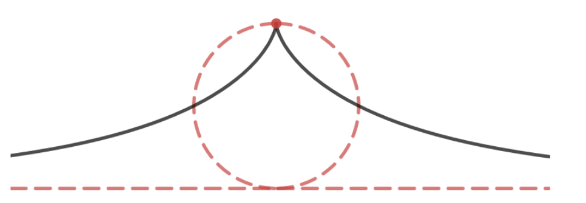
\includegraphics[width=0.7\textwidth]{CissoidDiocles}
    \end{center}
    %
    The name cissoid originates from the Greek \textkappa \textiota \textsigma \textsigma \textomikron \textepsilon \textiota \textdelta \texteta \textvarsigma, meaning `ivy shaped`, probably because of the singular, or cuspal points common in the curves, like in the cissoid of Diocles. We can also describe the cissoid of Diocles by letting a point $P$ range over all points on the circle, and then obtaining a point $Q$ by first reflecting $P$ across the line parallel to the fixed tangent bisecting the circle to obtain a point $P'$, and then intersecting the line $OP$ with the line through $P'$ parallel to the tangent. The easiest way to see why this is true is to look at the diagram below, and use similarity of triangles.
    %
    \begin{center}
        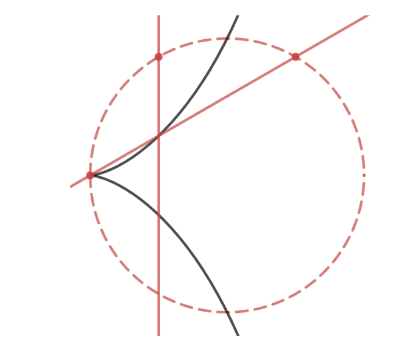
\includegraphics[width=0.4\textwidth]{CissoidDiocles2}
    \end{center}
    %
    If we consider a coordinate system in which $O$ lies at the origin, the circle is the unit circle with center $(1,0)$, and the tangent is the line described by the equation $x = 2$, then in polar coordinates, we may write the points on the circle as the solutions to the equation $r = 2 \sec \theta$, and the points on the tangent as solutions to $r = 2 \cos \theta$. The distance between the tangent line and the circle for a fixed angle $\theta$ is the difference in radii, which is just $2 \sec \theta - 2 \cos \theta$, and therefore the polar equation defining the cissoid of Diocles is
    %
    \[ r = 2(\sec t - \cos t) = \frac{2 - 2\cos^2 t}{\cos t} = \frac{2 \sin^2 t}{\cos t}\]
    %
    In cartesian coordinates we have $x = r \cos t$, $y = r \sin t$, and $r^2 = x^2 + y^2$, in cartesian coordinates this equation becomes
    %
    \[ x = \frac{2y}{x^2 + y^2} \]
    %
    so the cissoid of Diocles is the locus of points defined by the polynomial equation $(x^2 + y^2) x = 2y^2$, and is therefore an algebraic planar curve.
\end{example}

\begin{example}
    Another construction of Diocles' cissoid was discovered by Newton. Consider a rigid right angled joint forced to pass through a point $O$, and another point $P$ lying on a line not passing through $O$, where the length of the joint from the bend to the point $P$ is fixed, but the length through $O$ is allowed to vary. As we move the point $P$ along the line, the joint slides back and forth through the point $O$. If we take the midpoints $Q$ between the point $P$ and the bend in the joint, then we obtain the cissoid of Diocles. We have expressed Diocles' cissoid as a \emph{conchoid}, which is constructed from a general point $O$ and curve by taking points on lines through $O$ lying at a fixed distance from the curve. In this case, the curve is a line, and the distance is half the distance between the point and the line.
%
    \begin{center}
        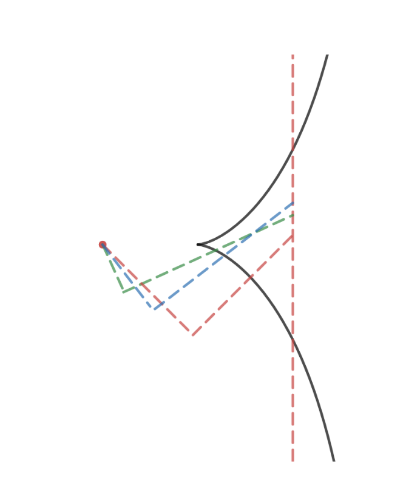
\includegraphics[width=0.4\textwidth]{ConchoidDiocles}
    \end{center}
%
    Suppose we choose a coordinate system in which $O = (-1,0)$, and the line over which $P$ varies is described by the equation $x = 1$. If $Q$ has coordinates $(a,b)$, and $P$ has coordinates $(1,p)$, then the fact that $OQP$ is a right angle is equivalent to saying that $\langle O - Q, P - Q \rangle = 0$, which gives the equation $a^2 + b^2 = 1 + bp$. The condition that $PQ$ has length 2 is equivalent to the algebraic equation $a^2 + b^2 + p^2 = 3 + 2a + 2bp$, which, assuming the first equation is satisfied, is equivalent to $p^2 = 2 + 2a + bp$. Introducing the midpoint $(X,Y)$ of $PQ$, which is the point we want to exist in the first place, we find that
    %
    \[ 2x = a + 1\ \ \ \ 2y = b + p \]
    %
    The first equation allows us to eliminate $a$ from the first two equations, and the second allows us to eliminate $b$. We obtain that the values of $x$ and $y$ which lie on the shape are exactly those such that there exists a value $p$ such that $(2x - 1)^2 + (2y - p)^2 = 1 + (2y - p)p$ and $p^2 = 2 + 2(2x - 1) + (2y - p)p$, which is simplified to the two equation $4x^2 + 4y^2 + 2p^2 = 6py + 4x$ and $p^2 = 2x + py$. Substituting the second equation into the first gives $x^2 + y^2 = py$, and substituting this equation back into the second, after multiplying the equation by $y^2$ on both sides gives $(x^2 + y^2)^2 = (2x + x^2 + y^2)y^2$, which can be simplified to $(x^2 + y^2)x = 2y^2$, so this constructing describes exactly the cissoid of Diocles.
    %
    \begin{center}
        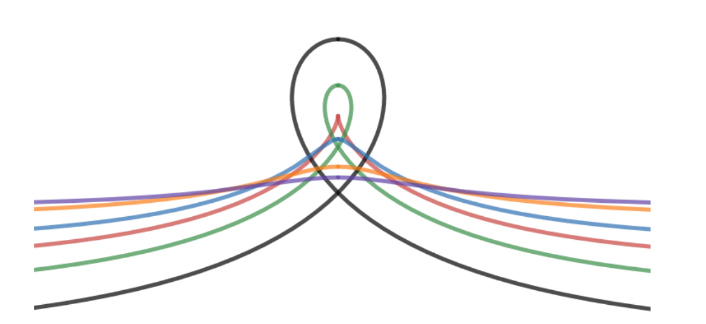
\includegraphics[width=0.8\textwidth]{ConchoidDiocles2}
    \end{center}
    %
    The advantage of Newton's construction is that we can obtain a one-parameter family of conchoidal curves which are deformations of the cissoid of Diocles, by taking points on the joint lying at a different ratio than the midpoint. Indeed, if we write $x = ac + (1 - c)$ and $y = cb + (1 - c)p$, then provided that $c \neq 0$ we can still use the first equation to eliminate $a$, and use the second to eliminate $b$, obtaining that
    %
    \[ x^2 + y^2 + 2(c-1)x + p(c-2)y + (1 - c)p^2 = 2c - 1\ \ \ \ \  p^2 = 2x + py + 4c - 2 \]
    %
    Substituting the second equation into the first gives $py = x^2 + y^2 - 4c^2 + 4c - 1$, and substituting the equation back into the second once multiplying by $y$ on both sides of the equation gives
    %
    \[ x^4 + x^2y^2  - 2xy^2 - 2(2c-1)^2x^2 + (1 - 4c^2)y^2 = -16c^4 + 32c^3 - 24c^2 + 8c - 1 \]
    %
    These are quartic curves, which for $c < 1/2$ have a `loop' singularity, and are smooth for $c > 1/2$. The polynomial equations defining the quartic conchoids of Diocles are quartic, but we can obtain similar behavior in the cubic sense. These are the conchoids of de Sluze, described by the equation $(x-1)(x^2 + y^2) = ax^2$, which is equal to the conchoid of Diocles when $a = -1$.
    %
    \begin{center}
        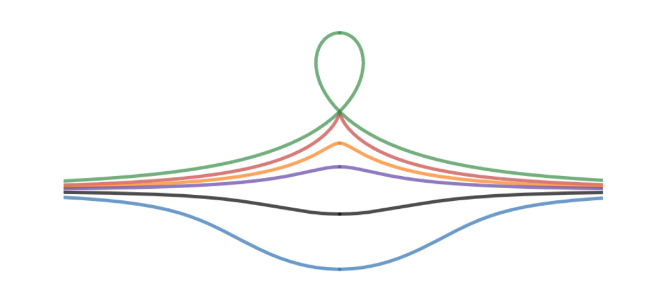
\includegraphics[width=0.7\textwidth]{ConchoidDesluze}
    \end{center}
\end{example}

\begin{example}
    Another example of an algebraic plane curve is the conchoid of D\"{u}rer, obtained by taking a pair of perpendicular lines intersecting at a point $O$, considering points $Q$ and $R$ moving on these lines such that the sum of the distances from $O$ to $Q$ and $O$ to $R$ is constant, and then taking the point on $QR$ at a fixed distance from $Q$. If we take the perpendicular lines as the $X$ and $Y$ axis, with $O$ the origin, take $b$ as the sum of distances, and take $a$ as the distance from $Q$, then each point $(X,Y)$ lies on the curve if, first, it lies on a line $PQ$, where $Q = (x,0)$ and $P = (0,y)$, where $yX + xY = xy$, such that $x + y = b$, and $(X - x)^2 + Y^2 = a^2$. We can eliminate $y$ from the equation since we can write $y = b -x$, so that $(b-x)X + xY = x(b-x)$. For a fixed $X$ and $Y$, this equation is quadratic in $x$, which can be rewritten as $x^2 + bX = x(b + X - Y)$. The equation $(X - x)^2 + Y^2 = a^2$ gives $x^2 = a^2 - Y^2 - X^2 + 2xX$, hence $a^2 - Y^2 - X^2 + bX = x(b - X - Y)$, which gives $(b - X - Y)x = a^2 - Y^2 - X^2 + bX$. Finally, we obtain the constraints on $X$ and $Y$ by multiplying the equation $(b - x)X + xY = x(b - x)$ on both sides by $(b - X - Y)^2$ allows us to eliminate the remaining values of $x$, which can be rearranged to give the equation
    %
    \[ 2y^2(x^2 + y^2) + (b^2 - 3a^2)y^2 + 2a^2b(x + y) + a^2(a^2 - b^2) = a^2x^2 + 2by^2(x + y) \]
    %
    so the curve is a quartic curve. For $b = 0$, the curve becomes a pair of lines together with a circle, and for $a = 0$, we obtain two coincident straight lines.
    %
    \begin{center}
        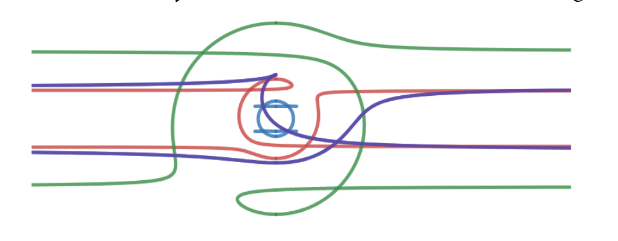
\includegraphics[width=0.7\textwidth]{ConchoidDurer}
    \end{center}
\end{example}

\begin{example}
    The conchoid of Nicomedes is obtained by fixing a point $P$, and letting $Q$ vary over a line not containing $P$. For each $Q$, the conchoid consists of the points on the line $PQ$ at a fixed distance away from $Q$. If $P$ lies at the origin, $Q$ varies along the line described by the equation $y = a$, and the distance parameter is $b$, then the equation describing the conchoid is
    %
    \[ (y-a)^2(x^2 + y^2) = b^2y^2. \]
    %
    The conchoids appear to take three different forms depending on the relation between the distance between $P$ and the line, and the distance defining the conchoid. If $a > b$, we obtain two smooth curves. If $a < b$, the conchoid appears to `swing' around the point $P$, with $P$ as a nodal point. If $a = b$, then we obtain a `cusp' at $P$. An interesting feature of the conchoid of Nicomedes is that it is \emph{isochronous}; the time for an object to reach the `bottom' of the conchoid under the influence of gravity starting from zero velocity is independent of it's original starting position on the curve.
    %
    \begin{center}
        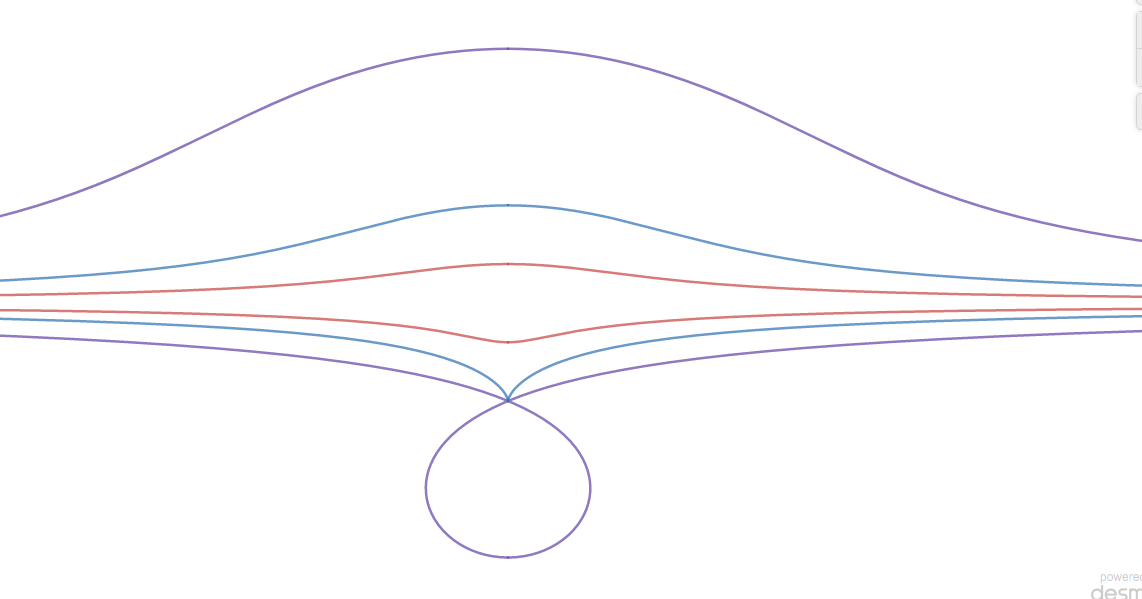
\includegraphics[width=0.7\textwidth]{ConchoidNicomedes.png}
    \end{center}
    %
    the time for an object to reach the `bottom' of the conchoid under the influence of gravity is independent of its original starting position.
\end{example}

\begin{example}
    Just as we can obtain the conic sections by intersecting a cone with a parabola, the spiric sections of perseus are obtained by intersecting a plane with a torus. The general form of an equation describing a spiric section is of the form $(x^2 + y^2)^2 = dx^2 + ey^2 + f$.
    %
    \begin{center}
        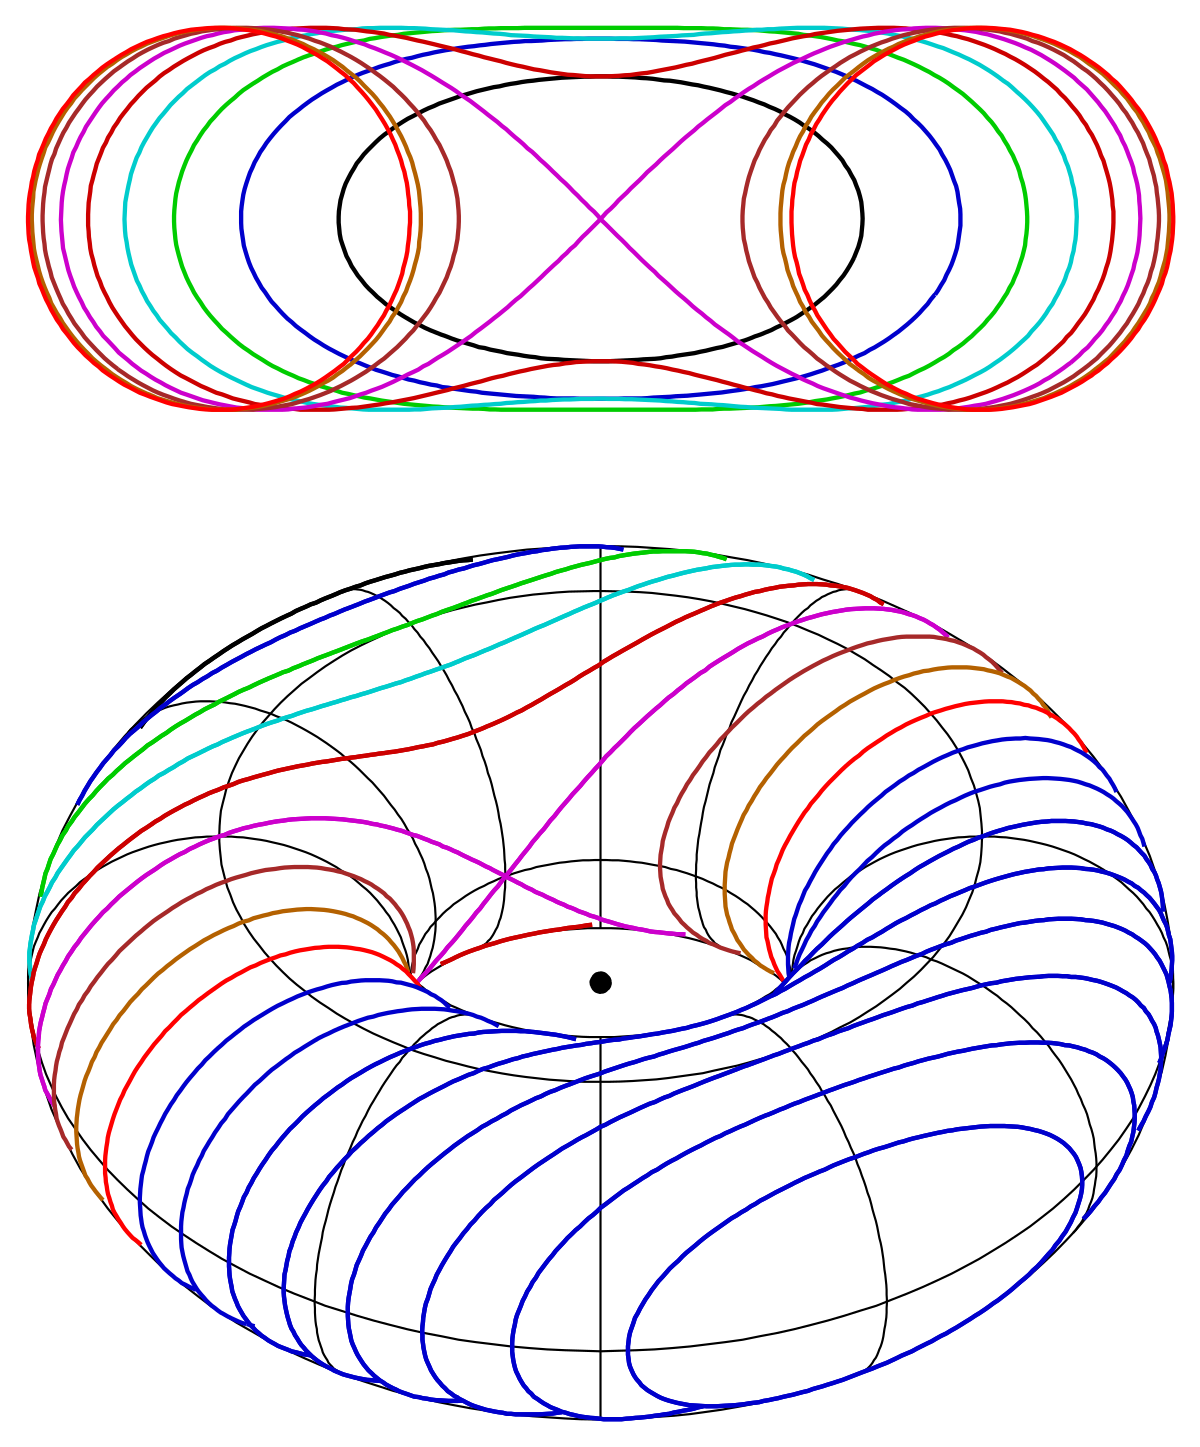
\includegraphics[width=0.7\textwidth]{SpiricSection.png}
    \end{center}
    %
    A particular family of spiric sections include the Cassini curves. These can be constructed by taking two focal points $P$ and $Q$, and considering the locus of points such that the product of the distances to $P$ and to $Q$ are a fixed quantity. If we fix the focal points at $(-1,0)$ and $(1,0)$, then an equation for the Cassini curve is $(x^2 + y^2)^2 - 2(x^2 - y^2) + 1 = a^4$, where $a$ is the distance parameter to the curve. Cassini was an astronomer who believed the sun rotated around the earth according to these curves. The curves are smooth, except if we let the distance $a$ be equal to $1$, in which case the point $(0,0)$ is singular since the curve intersects twice here. This curve is the lemniscate of Bernoulli, described by the equation $(x^2 + y^2)^2 = 2(x^2 - y^2)$.
\end{example}

\begin{example}
    The folium of Descartes is the algebraic curve defined by the equation $x^3 + y^3 = 3xy$. It's claim to fame is that the curve lead to the discovery of the method of implicit differentiation. In 1638, Descartes challenged Fermat to find the tangent line to the curve at any point on the circle, and with some primordial techniques of the calculus, Fermat was able to derive the tangent line at an arbitrary point.
    %
    \begin{center}
        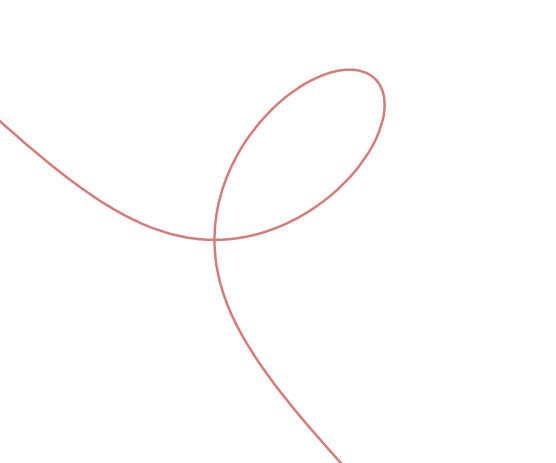
\includegraphics[width=0.7\textwidth]{FoliumDescartes.png}
    \end{center}
\end{example}

\begin{example}
    If we consider a circle lying on the outside of a circle, and we fix a point on the circle as it rotates around the circle, then provided that the circumference of the outer circle is a rational multiple of the circumference of the inner circle, we obtain an algebraic curve known as an epicycloid, and the rational multiple determined the period of rotation of the circle. If the inner circle has radius $R$, and the outer circle radius $r$, then we have a parameterization given by
    %
    \[ \left( (r + R) \cos t - r \cos \left(\frac{r + R}{r}t \right), (r + R) \sin t - r \sin \left( \frac{r + R}{r}t \right) \right) \]
    %
    If the circumference of the inner circle is equal to the circumference of the outer circle, the outer circle completes a single rotation before returning to its original location, and this curve is known as a cardoid, because it has a single cusp which looks like a heart. If the outer circle has half the circumference as the inner circle, the outer circle rotates twice before returning to its original position, and we obtain a function with a single cusp, and we call this shape a nephroid, since the shape looks like a kidney. Similarly, the hypocycloids are obtained by revolving a circle along the interior of the circle. If we revolve the outer circle around the inner circle, we obtain a pericycloid. If we fix a general point on these circles, we obtain the trochoids.
\end{example}

Algebraic curves are a rich source of geometric problems. For this reason, they inspired the general theory of algebraic geometry. Here are some natural questions we can ask about algebraic curves:
%
\begin{itemize}
    \item Is it possible to parameterize an algebraic curve's points by a rational function of a single argument? We call such curves \emph{rational curves}. This is more difficult than it seems. For instance, the algebraic curve described by the equation $y^2 = x^2 + x^3$ has a rational parameterization. For each value of $t$, the line $y = tx$ intersects the curve in a single position outside of the origin, because the solutions are given by nonzero values of $x$ such that $(tx)^2 = x^2 + x^3$, so that $(t^2 - 1)x^2 = x^3$, so $x = t^2 - 1$, $y = t^3 - t$ gives the unique point off the origin on the line $y = tx$. But since every point on $y^2 = x^2 + x^3$ lies on some line through the origin, we find that $(t^2 - 1, t^3 - t)$ gives a parameterization of the curve. This is not just a novel problem, because if we wish to perform an integration
    %
    \[ \int \varphi \left(x, \sqrt{x^2 + x^3} \right) dx\ \ \ \ \ \int \varphi \left( x, - \sqrt{x^2 + x^3} \right) dx \]
    %
    where $\varphi$ is a rational function in two variables, then we know that the substitution $x = t^2 - 1$ gives $\sqrt{x^2 + x^3} = t(t^2 - 1)$, so we are reduced to performing the integration
    %
    \[ \int \varphi(t^2 - 1, t(t^2 - 1)) 2t\; dt \]
    %
    Thus the antiderivative of every rational function of $x$ and $\sqrt{x^2 + x^3}$ is expressible in elementary terms. On the other hand, the cubic curve described by the equation $y^2 = x^3 + 1$ is not parameterized by a rational function of a single variable, and this is closely related to the fact that the integral
    %
    \[ \int \frac{dx}{\sqrt{x^3 + 1}} \]
    %
    is not expressible in terms of elementary functions.

    \item Another reason to study rational curves is to determine the points on a curve with rational coefficients. For instance, we can consider the rational solutions to the curve described by the equation $y^2 = x^2 + x^3$. We know that for each $t \in \mathbf{Q}$, $(t^2 - 1, t(t^2 - 1))$ gives a point on the curve with rational coordinates. Conversely, if $(t^2 - 1, t(t^2 - 1))$ is a rational coordinate, then $t^2$ is a rational number, and provided that $t^2 - 1 \neq 0$, we conclude that $t$ is also a rational number. On the other hand, if $t^2 - 1 = 0$, then $t = \pm 1$ is obviously rational. Thus we can obtain all rational points on the curve by taking the function of a single rational number. Fermat's last theorem asks us to determine whether the equation $x^n + y^n = z^n$ has any integer solutions for $n > 2$, which is equivalent to the existence of rational solutions to the equation $x^n + y^n = 1$, so the problem is very closely related to problems about algebraic curves.

    \item It is an important problem in geometry to classify geometric objects. The classical way to identify two curves is if they are equal to one another once we change our coordinate system. One invariant of this process is the \emph{degree} of the curve, that is, the degree of the polynomial defining the curve. Thus we have degree one curves, which are lines, the degree two curves, the conics, which are after discounting degenerate solutions, classified into parabolas, hyperbolas, and ellipses. But the cubics give a whole new world; Newton gave a classification of the cubic curves into 72 families; Pl\"{u}cker into a more systematic 219 class system.

    To simplify the situation, we can `weaken' the classification we use. If we view algebraic curves as lying in projective space rather than affine space, and identify curves by changing projective coordinates rather than affine coordinates, then the ellipse, hyperbola, and parabola are all identified as the same family of curves. We can imagine that the classification of cubics is also simplified considerably.

    Another way to simplify this situation is to identify two curves which are `intrinsically the same', in the sense that we can map one curve onto another by a coordinate map given by polynomial equations, whose inverse can also be specified by polynomial equations. We call these isomorphisms \emph{regular maps}. If we identify curves by rational functions rather than polynomials, we obtain the \emph{birational maps} between curves. The curves birationally equivalent to a line are exactly the rational curves. These are the basic notions leading to the intrinsic theory of algebraic geometry.
\end{itemize}
%
Polynomials, being a rather restricted class of functions, defined a class of fairly well behaved curves. Aside from the class of smooth curves, however, they possess certain irregularities.
%
\begin{itemize}
    \item Algebraic curves can have \emph{singular points} where the curve is no longer `smooth'. If an algebraic curve is defined with respect to a polynomial $f$, and $(\nabla f)(p) \neq 0$ where $f(p) = 0$, then we can locally describe one coordinate on the curve as a function of another curve, so the curve is smooth. But it is entirely possible for $(\nabla f)(p)$ to vanish, in which case the algebraic curve no longer behaves smoothly. One reason this can occur is if the algebraic curve has a \emph{node}, which occurs if $p$ is the intersection point of two smooth branches of the curve. Another reason is if the function rapidly changes direction, in which case we have a \emph{cusp}. Unless we restrict the class of algebraic curves we are considering to the \emph{non-singular} curves, then there is no way to avoid this issue, and we must face singular points head on.

    \item The zero sets of some polynomials do not have `curve-like' solutions at all. For instance, the equation $x^2 + y^2 = 0$ has only a single solution $(0,0)$, so given our present definition we have to agree that the set $\{ (0,0) \}$ is an algebraic curve. This annoyance disappears when we study algebraic plane curves over the complex numbers, whose algebraic completeness means that $x^2 + y^2$ factors into $(x + iy)(x - iy)$, so the solution set is the union of two planes, known as \emph{complex lines}, through the origin, so the solution set behaves locally like a two dimensional space. A two-dimensional space is `one-dimensional' over the complex numbers, so the solution set over the complex numbers behaves like a \emph{complex curve}. This is where the theory of Riemann surfaces enter the picture (since a one dimensional complex curve is a two dimensional real surface), and we find an interesting interplay between analytic and algebraic viewpoints.
\end{itemize}
%
On the other hand, being of essentially algebraic character, most of the basic techniques can be formalized to study algebraic curves over any field. In general, we shall assume some field $k$ is fixed, which throughout this part of the notes we assume to be \emph{algebraically closed}; the most elementary object of study will be the $n$ dimensional affine space $\mathbf{A}^n$ over the field $k$, which can be identified with the space $k^n$ of $n$ tuples of field elements after a coordinate system is fixed. $\mathbf{A}^1$ is referred to colloquially as the affine line, and $\mathbf{A}^2$ as the affine plane. On a first glance, geometric intuition appears to break down over fields of finite characteristic, or other abstract fields, but surprisingly, the arguments which justify certain solutions to algebraic geometry over the complex numbers generalize to most other fields. Working in the algebraically closed setting can allow us to infer insights that weren't present working solely over another field.

\begin{example}
    Here is an example where working over the complex numbers enables us to prove relations about geometry in the Euclidean plane. If $p$ is a point outside a circle $C$, then it lies on precisely two tangent lines to the circle. We define the \emph{polar line} to be the line through the two points on the circle whose tangents pass through $p$.

    If we assume without loss of generality that our circle is described by the equation $x^2 + y^2 = 1$, then for each point $q = (q_1,q_2) \in C$, the tangent line $L_q$ to $C$ at the point $q$ is described by the equation $q_1x + q_2y = 1$. If $p = (a,b)$, then the pair of points $q$ such that $p \in L_q$ is precisely the family of points such that $ax + by = 1$ and $x^2 + y^2 = 1$. Multiplying this second equation by $a^2$ and substituting $1 - by$ for $ax$, we conclude that
    %
    \[ (a^2 + b^2)y^2 - 2by + (1 - a^2) = 0 \]
    %
    The discriminant of this equation is $4a^2(a^2 + b^2 - 1)$, and so this equation has two distinct solutions provided that $a^2 + b^2 > 1$.

    If the point $p$ lies on the interior of the circle $C$, then $0 < a^2 + b^2 < 1$, then the discriminant is negative, which implies that $p$ lies on no tangent to the circle. On the other hand, we can still solve these equations to determine two complex points on the `complex circle'. The coordinates of the two complex points we find must be conjugates of each other, and so if $(x,y)$ is one of these points then the line between these two points is given by
    %
    \[ (\overline{x} - x)(Y - y) = (X - x)(\overline{y} - y) \]
    %
    Simplifying, the line is described by the equation
    %
    \[ \text{Im}(x) Y - \text{Im}(y) X = \text{Im}(x) \text{Re}(y) - \text{Im}(y) \text{Re}(x) \]
    %
    a purely real line, which can still be interpreted in a polar sense. Geometrically, it is the locus of all points whose polar line passes through $p$. Thus we are lead to a construction which would not have seemed so simple would we have restricted ourselves to real space, and it leads naturally to an exploration of the theory of inversive geometry.
\end{example}

We shall return to the study of algebraic plane curves after we introduce some general tools from the framework of algebraic geometry. But algebraic curves still provide a nice source of simple, but nontrivial examples of which to try out the general theory.

\section{Affine Varieties}

Given a polynomial $f \in k[X_1, \dots, X_n]$, we can consider the set of zeroes of $f$ as a geometric shape, i.e. the set
%
\[ Z(f) = \{ p \in \mathbf{A}^n : f(p) = 0 \}. \]
%
We call $Z(f)$ the \emph{algebraic hypersurface} defined by $f$. We can also consider the geometric set obtained from the common zeroes of two polynomials $Z(f,g) = Z(f) \cap Z(g)$. More generally, given a set $S$ of polynomials, we can consider the \emph{zero set of $S$}, denoted by $Z(S)$, which consists of the common zeroes of all polynomials in $S$. Sets formed from $\mathbf{A}^n$ by taking the zero set of a family of polynomials are called \emph{affine algebraic sets}.

%Let us consider some elementary geometric properties.

%Being invariant under affine transformations, the class of affine varieties is interesting from the point of Euclidean geometry. Many interesting shapes which occur in classical Euclidean geometry can be identified with varieties, through the tools of analytic geometry. If $T$ is an affine transformation on $\mathbf{A}^n$, we define the endomorphism $T^*$ on $k[X_1,\dots,X_n]$ by letting $T^*f = f \circ T$. Then $T^{-1}(Z(S)) = Z(T^* S)$, so the two shapes are essentially equal. It is easy to prove that $T^*$ preserves the degree of polynomials, which is one of the reasons why the degree of polynomials is an {\it isomorphism-invariant} property of algebraic curves, when our isomorphisms are obtained by affine transformations. Affine transformations are the most basic classes of isomorphisms of algebraic varieties.

%\begin{theorem}
%    An algebraic hypersurface $\Sigma$ in $\mathbf{A}^n$ specified by a polynomial of degree $d$ either contains a line, or intersects it in at most $d$ places.
%\end{theorem}
%\begin{proof}
%    Let $\Sigma$ be specified as the locus of a polynomial $f$. Fix $x_0,t_0 \in k$. For any  line $L$ described by some equation $X = x_0 + t_0Y$, the points on $\Sigma \cap L$ are in one to one correspondence with the zeroes of the polynomial $g(Y) = f(x_0 + t_0Y,Y) \in k[Y]$, and $\deg(g) \leq \deg(f) = d$. thus, unless $g = 0$, in which case $\Sigma$ contains $L$, the surface $\Sigma$ intersects $L$ in at most $d$ places.
%\end{proof}

%\begin{remark}
%    A simple consequence of this theorem is that
    %
%    \[ \{ (x,y) \in \mathbf{R}^2 : y = \sin(x) \} \]
    %
%    is not an algebraic curve in $\mathbf{R}^2$, since it intersects the $x$-axis infinitely many times but does not contain the $x$-axis. Neither is the set
    %
%    \[ \{ (z,w) \in \mathbf{C}^2 : |z|^2 + |w|^2 = 1 \} \]
    %
%    since the intersection of the complex sphere with the $z$ axis is a circle, which has infinitely many points.
%\end{remark}

There are some elementary observations we can make on the association $S \mapsto Z(S)$, which open the floodworks to reducing geometric problems on an algebraic set to the algebraic problems on the ring $k[X_1, \dots, X_n]$.
%
\begin{itemize}
    \item If $S \subset T$, then $Z(T) \subset Z(S)$.

    \item If $\mathfrak{a}$ is the smallest ideal containing $S$, then $Z(S) = Z(\mathfrak{a})$, so every affine algebraic set can be described as the common zeroes of some ideal in $k[X_1,\dots,X_n]$.

    \item If we have a family $\{ \mathfrak{a}_\alpha \}$ of ideals, then $Z(\bigoplus \mathfrak{a}_\alpha) = \bigcap Z(\mathfrak{a}_\alpha)$, so the intersection of an arbitrary family of algebraic sets is an algebraic set.

    \item For any two polynomials $f$ and $g$, $Z(fg) = Z(f) \cup Z(g)$. More generally, if $\mathfrak{a}$ and $\mathfrak{b}$ are ideals, then $Z(\mathfrak{a}\mathfrak{b}) = Z(\mathfrak{a}) \cup Z(\mathfrak{b})$, so finite unions of algebraic sets are algebraic sets.

    \item $Z(0) = \mathbf{A}^n$, $Z(1) = \emptyset$, and for any $a \in k^n$, $Z(X_1-a_1,\dots,X_n - a_n)$ is just the singleton set $\{ a \}$. It follows from the last point that any finite set of points is an algebraic set.
\end{itemize}

Conversely, if $X$ is any subset of $\mathbf{A}^n$, then we shall let $I(X)$ be the subset of $k[X_1, \dots, X_n]$ of polynomials which vanish over $X$. The set $I(X)$ forms an ideal, and it is clear that in the case where $X = Z(S)$, the ideal contains all elements of $S$, hence all elements of $\mathfrak{a}$. The generation of an ideal $I(X)$ from a set $X$ is dual to the notion of generating a set $Z(\mathfrak{a})$ from an ideal $\mathfrak{a}$. We make a few elementary observations about this operator.
%
\begin{itemize}
    \item If $X \subset Y$, then $I(Y) \subset I(X)$.
    \item $I(\emptyset) = k[X_1, \dots, X_n]$, and $I(\mathbf{A}^n) = (0)$.
    \item $S \subset I(Z(S))$ for any subset $S$ of polynomials, and $X \subset Z(I(X))$. In fact, $Z(I(X))$ is the smallest algebraic set in $\mathbf{A}^n$ containing $X$, the \emph{Zariski closure} of $X$.
    \item The last point implies that for any algebraic set $X$, $Z(I(X)) = X$.%It is simple to see that $V \subset Z(I(Z))$. Conversely, if $V = Z(S)$ for some $S \subset k[X_1,\dots,X_n]$, then $S \subset I(V)$, so $Z(I(V)) \subset Z(S) = V$. Similarily, if $\IA$ is an ideal in $k[X_1,\dots,X_n]$ which is equal to $I(X)$ for some set $X$, then $I(Z(\IA)) = \mathfrak{a}$.
    \item If $f \in k[X_1,\dots,X_n]$ and $f^k \in I(X)$ for some $k$, then $f \in I(X)$. This means exactly that $I(X)$ is a \emph{radical ideal} of $k[X_1,\dots,X_n]$. The smallest radical ideal containing some ideal $\IA$ will be denoted by $\text{Rad}(\IA)$.
\end{itemize}

\begin{prop}
    If $X$ and $Y$ are distinct algebraic sets, then $I(X) \neq I(Y)$.
\end{prop}
\begin{proof}
    This follows because $Z(I(X)) = X$ and $Z(I(Y)) = Y$.
\end{proof}

The largest heuristic that guides the subject of algebraic geometry is that when $k$ is algebraically closed, geometric properties of a algebraic set are completely summarized in the algebraic structure of the ring of functions $k[X_1,\dots,X_n]$ acting on this algebraic set; the most central result here is Hilbert's Nullstellensatz, which gives an exact correspondence between algebraic sets in $\mathbf{A}^n$ and \emph{radical} ideals in $k[X_1,\dots,X_n]$, via the correspondence $X \mapsto Z(X)$ and $\IA \mapsto I(\IA)$. We will discuss the Nullstellensatz later on in this chapter.

\begin{theorem}
    If $X$ is an algebraic set in $\mathbf{A}^n$, and $p \not \in X$, then there is a polynomial $f \in I(X)$ with $f(p) = 1$.
\end{theorem}
\begin{proof}
    Since $X$ and $X \cup \{ p \}$ are distinct algebraic sets, $I(X) - I(X \cup \{ p \})$ is nonempty, so there must be a polynomial $f$ vanishing on $X$, but with $f(p) \neq 0$. By normalizing we can assume $f(p) = 1$.
\end{proof}

Similarly, by taking an algebraic set $X$, and $n$ points $p_1, \dots, p_n \not \in X$, we can repeatedly use this theorem to find polynomials $f_1, \dots, f_n \in I(V)$ with $f_i(p_j) = \delta_{ij}$ for each $1 \leq i,j \leq n$. By considering linear combinations of the $f_i$, for any $a_{ij} \in k$, we can find $f_1, \dots, f_n \in I(X)$ with $f_i(p_j) = a_{ij}$. This shows the space of polynomials which vanish over $X$ has enough degrees of freedom to specify values on a finite set of points outside of $X$. An immediate consequence of this is that the Zariski topology, defined in the next section, is T1.

Recall that $k[X_1,\dots,X_n]$ is a \emph{Noetherian ring}; any ideal in $k[X_1,\dots,X_n]$ is finitely generated. Since any algebraic algebraic set is formed from the common zeroes of polynomials found in an ideal $\mathfrak{a}$ of $k[X_1,\dots,X_n]$, it follows that the geometric consequence of a ring being Noetherian is that any algebraic set is formed from the common zeroes of a \emph{finite family} of polynomials. Thus the class of algebraic sets has a combinatorial nature not found in other families of surfaces, like the space of smooth surfaces.

\section{The Zariski Topology}

Note that, since the finite union of algebraic sets is an algebraic set, and the infinite intersection of algebraic sets is an algebraic set, the family of algebraic sets form the family of \emph{closed sets} for a topology on $\mathbf{A}^n$. This topology is known as the \emph{Zariski topology on $\mathbf{A}^n$}. More generally, we can induce the Zariski topology on any affine algebraic set $X$, and this is the same as declaring all algebraic subsets of $X$ to be closed. The Zariski topology is \emph{not} Hausdorff, which makes it slightly unintuitive to work with at first, but it a useful shorthand to describe many geometric properties of a ring.

\begin{example}
    The algebraic subsets of $\mathbf{A}^1$ are exactly the finite point sets, aside from $\mathbf{A}^1$ itself. This is because any polynomial $f \in k[X]$ has only finitely many zeroes. In terms of the Zariski topology, this means that $\mathbf{A}^1$ has the \emph{cofinite topology}; a proper subset of $\mathbf{A}^1$ is Zariski open if and only if it's complement is finite.
\end{example}

For any $f \in k[X_1,\dots,X_n]$, the set
%
\[ D(f) = \{ p \in \mathbf{A}^n: f(p) \neq 0 \} \]
%
is a Zariski open set in $\mathbf{A}^n$. Conversely, if $U$ is any Zariski open set, then there exists $f_1,\dots,f_n \in k[X_1,\dots,X_n]$ such that $U^c = Z(f_1,\dots,f_n)$, i.e. that $U^c = Z(f_1) \cap \dots \cap Z(f_n)$, and so $U = D(f_1) \cup \dots \cup D(f_n)$. Thus the family of sets $\{ D(f): f \in k[X_1,\dots,X_n] \}$ are a \emph{basis} for the Zariski topology, and every Zariski open set can be written as a finite union of these sets. Open sets of the form $D(f)$ for some $f \in k[X_1,\dots,X_n]$ are known as \emph{basic}, or \emph{distinguished} open sets. More generally, given an algebraic set $X = Z(S)$, and a polynomial $f \in k[X_1,\dots,X_n]$, we define $U_X(f) = \{ p \in X : f(p) \neq 0 \}$, which is a Zariski open subset of $X$. These sets also form a basis for the Zariski topology on $X$.

\begin{example}
    Any nonempty Zariski open subset of $\mathbf{A}^n$ contains infinitely many points. It suffices to show that $D(f)$ has infinitely many points for any nonzero polynomial. We can find a line $L$ in $\mathbf{A}^n$ described by an equation $Y = mX + b$ of $X = mY + b$ such that $f$ is nonconstant when restricted to $L$. Thus $f(X,mX + b)$ or $f(mY + b,Y)$ is nonconstant. But any nonconstant polynomial on $\mathbf{A}^n$ can have finitely many zeroes, so all but finitely many points on $L$ lie in $D(f)$. Since $L$ has infinitely many points, this completes the argument.
\end{example}

\begin{example}
    If $n \geq 2$, and $f \in k[X_1,\dots,X_n]$ is a nonconstant polynomial, then $Z(f)$ is infinite. We argue like the previous example. Given $f$, there is a plan upon which $f$ is nonconstant, and it suffices to argue the theorem in two dimensions, i.e. for $f \in k[X,Y]$. Write
    %
    \[ f = \sum_{i = 0}^m \sum_{j = 0}^m a_{ij} X^i Y^j. \]
    %
    Without loss of generality, we may assume $f(0) \neq 0$. For each $t \in k$, let $L_t$ be the line through the origin described by the equation $Y = tX$. Since the family of sets $L_t \cap Z(f)$ is disjoint, it suffices to show $L_t \cap Z(f)$ is nonempty for infinitely many $t$. But since $k$ is algebraic closure, $L_t \cap Z(f) \neq \emptyset$ if $f(X,tX)$ is a nonconstant polynomial in $k[X]$, which holds if there exists some $1 \leq k \leq 2m$ such that
    %
    \[ \sum_{i = 0}^m a_{i(k-i)} t^{k-i} \neq 0. \]
    %
    For a fixed $k$, unless $a_{i(k-i)} = 0$ for all $0 \leq i \leq m$, it follows that there are only finitely many $t$ which fail to have this property. It cannot be true that $a_{i(k-i)} = 0$ for all $0 \leq i \leq m$ and $1 \leq k \leq 2m$, because $f$ is a nonconstant polynomial.
\end{example}

%\begin{example}
%    The set
    %
%    \[ \{ (x,y) \in \mathbf{R}^2 : y = \sin(x) \} \]
    %
%    is \emph{not} an algebraic curve in $\mathbf{R}^2$. This can be verify by noting that any algebraic curve specified by a polynomial of degree $d$ intersects any line at most $d$ times, or contains the line. A similar argument shows the set
    %
%    \[ \{ (z,w) \in \mathbf{C}^2 : |z|^2 + |w|^2 = 1 \} \]
    %
%    is not an algebraic curve in $\mathbf{C}^2$, since the intersection of the complex sphere with the $z$ axis is a circle, which has infinitely many points.
%\end{example}

\section{Reducibility}

A nonempty topological space $X$ is said to be \emph{irreducible} if it cannot be written as the union of two proper closed subsets. By convention, the empty set is not considered to be irreducible.

\begin{example}
    $\mathbf{A}^1$ is irreducible since it's only proper closed subsets are finite, yet $\mathbf{A}^1$ itself is infinite.
\end{example}

Applying this notion to the Zariski topology, an algebraic set $X$ will be irreducible if and only if it cannot be written as the union of two proper algebraic subsets. An irreducible algebraic set will be called a \emph{variety}. Ring theory characterizes irreducibility of an algebraic set $X$ in terms of $I(X)$.

\begin{prop}
    An algebraic set $X$ is irreducible if and only if $I(X)$ is prime.
\end{prop}
\begin{proof}
    Suppose that $I(X)$ is not prime, so there is $f,g \in k[X_1,\dots,X_n]$ such that $fg \in I(X)$, but $f,g \not \in I(X)$. Then $\IA = (f,I(X))$ and $\IB = (g,I(X))$ are ideals containing $I(X)$. Let $Y = Z(\IA)$ and let $Z = Z(\IB)$. Then $Y$ and $Z$ are proper closed subsets of $X$. If $x \in X$, then $f(x) g(x) = 0$, implying either $f(x) = 0$ or $g(x) = 0$. Thus $X = Y \cup Z$, which shows that $X$ is reducible.

    Conversely, if $X$ is reducible, we can write $X = Y \cup Z$ for two proper closed subsets $Y$ and $Z$. Then $I(X)$ is a proper subset of $I(Y)$ and $I(Z)$, so we may select $f \in I(Y) - I(X)$ and $g \in I(Z) - I(X)$. Then $fg \in I(X)$, but $f,g \not \in I(X)$, which shows $I(X)$ is not prime.
\end{proof}

\begin{example}
    The parabola $V = Z(Y - X^2)$ is a variety. It is easy to verify that $Y - X^2$ is irreducible, and since $k[X,Y]$ is a unique factorization domain, this implies $(Y - X^2)$ is prime. Provided that $I(V) = (Y - X^2)$, this verifies that $V$ is irreducible. So suppose $f \in I(V)$. Then we may apply the division algorithm to write
    %
    \[ f = g (Y - X^2) + h, \]
    %
    for some $g \in k[X,Y]$ and $h \in k[X]$. Since $f \in I(V)$, $f(x,x^2) = 0$ for all $x \in k$, which implies $h(x) = 0$ for all $x \in k$; provided $k$ is infinite, this means $h = 0$, so $f$ is divisible by $Y - X^2$. Thus $I(V) = (Y - X^2)$.
\end{example}

\begin{theorem}
    Every nonempty open subset of an irreducible topological space is dense.
\end{theorem}
\begin{proof}
    If $X$ is an irreducible space, and $U$ is an open subset, then $X = U^c \cup \overline{U}$, so either $U^c = X$ or $\overline{U} = X$. But we cannot have $U^c = X$ since $U$ is nonempty, so $\overline{U} = X$.
\end{proof}

\begin{corollary}
    Any nonempty Zariski open subset of a variety is Zariski dense.
\end{corollary}

In most of mathematics, it is often a useful strategy to break objects into `atomic' components, understand these components, then understand the more general objects by forming these components back together. Algebraic geometry is no different, where it is often a useful strategy to break down algebraic sets into a finite union of varieties. The key idea behind this decomposition is exploiting the fact that $k[X_1,\dots,X_n]$ is Noetherian. Indeed, we refer to any topological space $X$ as \emph{Noetherian} if there exists no infinite decreasing chain of decreasing closed subsets in $X$.

\begin{lemma}
    Any affine algebraic set is Noetherian.
\end{lemma}
\begin{proof}
    Since any subset of a Noetherian topological space is Noetherian in the induced topology, it suffices to show that $\mathbf{A}^n$ is Noetherian for each $n$. But any decreasing chain $\{ X_i \}$ of closed subsets of $\mathbf{A}^n$ corresponds to an increasing chain $\{ I(X_i) \}$ of ideals in $k[X_1,\dots,X_n]$, which, because $k[X_1,\dots,X_n]$ is Noetherian, must be finite.
\end{proof}

%The idea behind this process is simple. If an algebraic set $V$ is not irreducible, then we can break it apart into two proper algebraic subsets $V_1 \cup W_1$. If $V_1$ is not irreducible, we can break it apart into two proper subsets $V_2 \cup W_2$. Thus we obtain a binary tree of algebraic subsets of $V$. Provided this binary tree is finite, the roots give a decomposition of $V$ into a finite family of varieties. That this binary tree is finite is guaranteed by the fact that $k[X_1, \dots, X_n]$ is Noetherian.

\begin{lemma}
    If $X$ is a nonempty Noetherian topological space, then there exists a unique family of irreducible closed subsets $\{ Y_1,\dots, Y_n \}$ such that $X = Y_1 \cup \dots \cup Y_n$, where $Y_i$ is not a subset of $Y_j$ for any $i \neq j$. The sets $\{ Y_i \}$ are called the \emph{irreducible components} of $X$.
\end{lemma}
\begin{proof}
    First we prove existence. Let $\mathcal{F}$ be the family of all nonempty closed subsets of $X$ which \emph{cannot} be written as a finite union of irreducible components. Then, because $X$ is Noetherian, $\mathcal{F}$ must have a minimal element $Y$. Since $Y \in \mathcal{F}$, the set $Y$ must not be irreducible, so we can write $Y = Y_1 \cup Y_2$, where $Y_1$ and $Y_2$ are closed subsets of $Y$. But then $Y_1,Y_2$ are not elements of $\mathcal{F}$, so they can be written as a finite union of irreducible components, and thus $Y$ can, which gives a contradiction.

    Now suppose $X = Y_1 \cup \dots \cup Y_n = Z_1 \cup \dots \cup Z_m$, where each of the sets $Y_i$ and $Z_j$ are closed, irreducible subsets of $X$. For each $i$, $Y_i = (Y_i \cap Z_1) \cup \dots \cup (Y_i \cap Z_m)$, so by irreducibility, $Y_i \cap Z_j = Y_i$ or $Y_i \cap Z_j = \emptyset$ for each $i$ and $j$. Similarily, $Y_i \cap Z_j = Z_j$ or $Y_i \cap Z_j = \emptyset$, so that $Y_i = Z_j$ or $Y_i \cap Z_j = \emptyset$. For a fixed $i$, we cannot have $Y_i \cap Z_j = \emptyset$ for all $j$, so there must exist some $j$ such that $Z_j = Y_i$. Thus $\{ Y_1,\dots,Y_n \} \subset \{ Z_1, \dots, Z_m \}$. But by symmetry, we also have $\{ Z_1,\dots,Z_m \} \subset \{ Y_1,\dots,Y_n \}$, which shows the irreducible decomposition is unique.
\end{proof}

\begin{corollary}
    Any affine algebraic set is the finite union of algebraic varieties.
\end{corollary}

%\begin{lemma}
%    If $\mathfrak{a}$ is an ideal of a Noetherian ring $A$, then out of the set of prime ideals containing $\mathfrak{a}$, there are only finitely many minimal ones.
%\end{lemma}
%\begin{proof}
%    If there was an ideal $\mathfrak{a}$ forming a counterexample to this lemma, then using the Noetherian property of $A$, there would certainly be a maximal such counterexample. The ideal $\mathfrak{a}$ could not be prime, because then there would only be a single minimal prime ideal containing $\mathfrak{a}$. Thus there is $x,y \in A$ with $xy \in I$, but with $x,y \not \in I$. Thus $(x) + \mathfrak{a}$ and $(y) + \mathfrak{a}$ are ideals bigger than $I$, and thus are not counterexamples to the theorem. Thus there are only finitely many prime ideals minimal with respect to contains $(x) + \mathfrak{a}$ and $(y) + \mathfrak{a}$ respectively. But if $\mathfrak{p}$ is a prime ideal containing $\mathfrak{a}$, then $xy \in \mathfrak{p}$, so either $x \in \mathfrak{p}$, or $y \in \mathfrak{p}$, implying that either $(x) + \mathfrak{a} \subset \mathfrak{p}$, or $(y) + \mathfrak{a} \subset \mathfrak{p}$. Thus a minimal prime ideal containing $\mathfrak{a}$ must be a minimal prime ideal in $(x) + \mathfrak{a}$ or $(y) + \mathfrak{a}$, which is a contradiction to the fact that there are infinitely many such prime ideals.
%\end{proof}

%\begin{theorem}
%    Every affine algebraic set can be written uniquely as the finite union of varieties, with no variety containing the other. These varieties are known as the \emph{irreducible components} of the algebraic set.
%\end{theorem}
%\begin{proof}
%    If $V$ is an algebraic set, there are only finitely many minimal prime ideals containing $I(V)$, and thus there are only finitely many maximal irreducible varieties contained in $V$. Now if $V$ can be written as the union of two families of varieties $V_1, \dots, V_N$ and $W_1, \dots, W_M$, then $V_n = \bigcup (V_n \cap W_m)$, so either $V_n \cap W_m = \emptyset$ or $V_n \cap W_m = V_n$, which implies $V_n \subset W_m$ for some $m$. Performing the same process in reverse gives $W_m \subset V_{n'}$ for some $n$, and obviously $n = n'$. By matching up elements of the decomposition, we conclude that the decomposition is unique.
%\end{proof}

\begin{example}
    Consider the algebraic set $X = Z(Y^4 - X^2, Y^4 - X^2Y^2 + XY^2 - X^3)$ in $\mathbf{C}^2$. Since $Y^4 - X^2 = (Y^2 - X)(Y^2 + X)$, we find
    %
    \begin{align*}
        Y^4 - X^2Y^2 + XY^2 - X^3 &= (Y + iX)(Y - iX)(Y-X)(Y+X)
    \end{align*}
    %
    Considering the zeroes which satisfy these equations on a case by case basis, we find that $X$ is just a set of discrete points, each an irreducible factor in the decomposition of $X$.
\end{example}

\begin{example}
    The polynomial $Y^2 + X^2(X-1)^2$ is irreducible over $\mathbf{R}[X,Y]$, but factors into $(Y + iX(X-1))(Y - iX(X-1))$ over $\mathbf{C}[X,Y]$. The consequence is that even though $Y^2 + X^2(X-1)^2$ is an irreducible polynomial, the algebraic set it generates is not irreducible, consisting of the two points $(0,0)$ and $(1,0)$. This is a consequence of the fact that over the real numbers,
    %
    \[ I(Z(Y^2 + X^2(X-1)^2) = (Y,X(X-1)) \neq (Y^2 + X^2(X - 1)^2) \]
    %
    is not a prime ideal.
\end{example}

In algebraic geometry we often say a topological space $X$ is \emph{quasi-compact} instead of compact, because in topological spaces that are not Hausdorff, compact sets do not behave quite as nicely than in spaces that are Hausdorff (for instance, a quasi-compact set need not be closed).

\begin{theorem}
    Every Noetherian topological space is quasi-compact.
\end{theorem}
\begin{proof}
    If $X$ is a Noetherian topological space, then every family of closed sets must have a minimal member. Thus if $\{ U_\alpha \}$ is an open cover of $X$, then the set of closed sets of the form $\{ X - U_{\alpha_1} - \dots - U_{\alpha_n} \}$ must have a minimal member, which must be the emptyset since the family $\{ U_\alpha \}$ covers $V$. This implies that any open cover of $X$ has a finite subcover, i.e. that $X$ is compact. 
\end{proof}

%\section{Dimensions of Varieties}

%The structure of $V$ we exploited above can be used to define a notion of \emph{dimension} to a variety. If $V$ is a variety, then there does not exist any infinite decreasing chain of Zariski closed sets (one verifies this easily using the Noetherian property of $k[X_1,\dots,X_n]$). We define the \emph{dimension} of a variety $V$ to be the largest $n$ such that there exists a chain
%
%\[ V_0 \supsetneq V_1 \supsetneq \dots \supsetneq V_n \]
%
%of irreducible subvarieties

%\begin{example}
 %   Since the only proper irreducible subsets of $\mathbf{A}^1$ are points, the largest chain of decreasing irreducible subvarieties is
    %
 %   \[ \mathbf{A}^1 \supset \{ 0 \} \]
    %
 %   Thus $\dim(\mathbf{A}^1) = 1$.
%\end{example}

\section{The Nullstellensatz}

In the last few sections, we have seen the duality between affine algebraic sets and radical ideals over the ring $k[X_1, \dots, X_n]$. Over algebraically closed fields, the correspondence between radical ideals and algebraic sets becomes exact. This is the content of Hilbert's Nullstellensatz theorem, which is a kind of generalization of the fundamental theorem of algebra.

%A precursor to the Nullstellensatz, known as Study's lemma will suffice for the study of planar algebraic curves.

%\begin{theorem}[Study]
%    If $k$ is algebraically closed, and $f,g \in k[X,Y]$ satisfy $Z(f) \subset Z(g)$, where $f$ is irreducible, then $f$ divides $g$.
%\end{theorem}
%\begin{proof}
%    If $f$ did not divide $g$, then $f$ and $g$ would be relatively prime, so $Z(f,g)$ consists of finitely many points. But $Z(f)$ is contained in $Z(f,g)$, which is impossible since $Z(f)$ contains infinitely many points.
%\end{proof}

%In terms of ideals, Study's lemma implies that if $f$ is a irreducible polynomials, then $I(Z(f)) = (f)$.
One consequence of the Nullstellensatz is that if $f$ is an irreducible polynomial, then $I(Z(f)) = (f)$; more generally, if $\IA$ is an ideal, and $f$ vanishes on the algebraic set $Z(\mathfrak{a})$, then $f^n \in \mathfrak{a}$ for some integer $n$. We begin with a `weak' form of the Nullstellensatz.

\begin{lemma}
    If $\mathfrak{a}$ is a proper ideal of $k[X_1, \dots, X_n]$, then $Z(\mathfrak{a}) \neq \emptyset$.
\end{lemma}
\begin{proof}
    We shall actually prove that if $\mathfrak{a}$ is a maximal ideal, then $Z(\mathfrak{a})$ is a set containing a single point. Since we may always extend every ideal to a maximal ideal, this will prove the proposition. So we take $\mathfrak{a}$ to be any maximal ideal. Then $k[X_1, \dots, X_n]/\mathfrak{a} = L$ is a field, which can be viewed as a field extension of $k$ because we can embed $k$ as the set of constant polynomials in $k[X_1, \dots, X_n]$. We write $x_i$ for the element of $L$ corresponding to $X_i$ in $k[X_1,\dots,X_n]$. If we knew that the embedding of $k$ in $L$ is an isomorphism, then for each $i$ there is $a_i \in k$ with $X_i - a_i \in \IA$. But this means that $\IA$ is equal to $(X_1 - a_1, \dots, X_n - a_n)$ since $\IA$ contains this ideal, which is maximal. It then follows that $Z(\mathfrak{a}) = \{ (a_1, \dots, a_n) \}$.
\end{proof}

\begin{remark}
    Our proof of the weak Nullstellensatz shows that the maximal ideal of $k[X_1,\dots,X_n]$ are in one to one correspondence with the points of $\mathbf{A}^n$, which is a very powerful property.
\end{remark}

%An important thing to note about this proof of the weak Nullstellensatz is that it implies that the maximal ideals of $k[X_1, \dots, X_n]$ are in one to one correspondence with the points of $\mathbf{A}^n$. The fact that maximal ideals are in one to one correspondence with points in space occurs in other context of mathematics, for instance, in the ring theory of $C(X)$, where $X$ is Hausdorff and locally compact. This point of view is often so useful that, when we study general rings $A$, we consider the set of maximal ideals of $A$ as points in a space, and then viewing elements of $A$ as functions on this space. This idea reoccurs later in our study of the local rings attached to algebraic sets, and in greater generality in the study of schemes.

To finish off the proof of the weak Nullstellensatz, it suffices to prove that if $k$ is an algebraically closed field, then for every field $L$ extension of $k$, for which there is a surjective homomorphism $k[X_1,\dots,X_n] \to L$, $k = L$. This is an easy consequence of Zariski's lemma, which we prove now.

\begin{lemma}
    Let $k$ be a field, and suppose $k[x_1, \dots, x_n]$ is a field. Then it is a finite extension of $k$.
\end{lemma}
\begin{proof}
    We prove this by induction on $n$. For $n = 1$, this is a classical argument in Galois theory. To continue the induction, suppose we have proved the theorem for all fields of the form $k[x_1, \dots, x_m]$, where $m < n$. We may then apply induction to $k[x_1, \dots, x_n] = k(x_1)[x_2, \dots, x_n]$ to conclude that $k[x_1, x_2, \dots, x_n]$ is a finite extension of $k(x_1)$. This means that there is some $k > 0$ and rational functions $a_0,\dots,a_{k-1} \in k(x_1)$ such that
    %
    \[ x_1^k = a_0 + a_1 x + \dots + a_{k-1} x^{k-1}. \]
    %
    Find a nonzero polynomial $b \in k[x_1]$ such that $ba_0,\dots,ba_{k-1} \in k[x_1]$. Then
    %
    \[ b x_1^k = a_0 b + a_1 b x + \dots + a_{k-1} b x^{k-1}. \]
    %
    This means that $x_1$ is algebraic over $k$, and therefore a finite extension of $k$. Thus $k[x_1]$ is a field, so we can apply induction to conclude that $k[x_1,\dots,x_n]$ is a finite extension of $k[x_1]$, and thus a finite extension of $k$.
\end{proof}

Since all finite extensions of a field are algebraic, if $k$ is algebraically closed then the last theorem implies $k[x_1,\dots,x_n] = k$. This finishes our proof of the weak Nullstellensatz. We now use the weak Nullstellensatz to prove the full Nullstellensatz.

\begin{theorem}
    Suppose $k$ is algebraically closed. If $\mathfrak{a}$ is an ideal in $k[X_1, \dots, X_n]$, then $I(Z(\mathfrak{a})) = \text{Rad}(\mathfrak{a})$, where $\text{Rad}(\mathfrak{a})$ is the set of all $f$ for which there exists $n$ with $f^n \in \mathfrak{a}$.
\end{theorem}
\begin{proof}
    Find $f_1,\dots,f_m \in k[X_1,\dots,X_n]$ such that $\IA = (f_1,\dots,f_m)$. We must show that if $g \in I(Z(\IA))$, there there are $h_1,\dots,h_m \in k[X_1,\dots,X_n]$ and an integer $k$ such that
    %
    \[ g^k = h_1f_1 + \dots + h_mf_m. \]
    %
    Without loss of generality, we may assume $g \neq 0$. Consider the ideal $\IB = (f_1, \dots, f_m, X_{n+1}g - 1)$ in $k[X_1,\dots,X_{n+1}]$. Then $Z(\IB) = \emptyset$, since if $x \in k^{n+1}$ and $f_i(x_1,\dots,x_n)$ for all $i$, then $g(x_1,\dots,x_n) = 0$, which implies that $x_{n+1}g(x_1,\dots,x_n) - 1 \neq 0$. The weak Nullstellensatz implies that $\IB = k[X_1,\dots,X_{n+1}$. Thus there are $a_1,\dots,a_m,b \in k[X_1,\dots,X_{n+1}]$ such that
    %
    \[ 1 = a_1f_1 + \dots + a_mf_m + b (X_{n+1} g - 1). \]
    %
    But this means that in $k(X_1,\dots,X_n)$,
    %
    \begin{align*}
        1 &= a_1(X_1,\dots,X_n,1/g) f_1 + \dots + a_m(X_1,\dots,X_n,1/g)\\
        &= \tilde{a}_1 f_1 + |dots + \tilde{a}_m f_m.
    \end{align*}
    %
    For a sufficiently large $k$, $c_1 = g^k \tilde{a}_1, \dots, c_k = g^k \tilde{a}_m$ are all elements of $k[X_1,\dots,X_n]$, and so it follows that in $k[X_1,\dots,X_n]$,
    %
    \[ g^k = c_1f_1 + \dots + c_mf_m, \]
    %
    which completes the proof.
\end{proof}

\begin{corollary}
    There is a one to one correspondence between radical ideals and algebraic sets in affine space over an algebraically closed field.
\end{corollary}

\begin{corollary}
    If $\mathfrak{a}$ is a prime ideal, then it is also a radical non total ideal, so $Z(\mathfrak{a})$ is an affine variety, and there is a one to one correspondence with such prime ideals and such varieties. The maximal ideals correspond to points in $\mathbf{A}^n$.
\end{corollary}

\begin{corollary}
    If $f \in k[X_1, \dots, X_n]$ has a decomposition as $f_1^{n_1} \dots f_m^{n_m}$, where $k$ is algebraically closed, then $Z(f) = Z(f_1 \dots f_n) = \bigcup Z(f_i)$ is the decomposition of $f$ into its irreducible factors. There is a one to one correspondence (up to scalar multiples) between irreducible hyperplanes and irreducible polynomials.
\end{corollary}

\begin{example}
    $V = Z(Y^2 - X(X-1)(X-\lambda))$ is a variety in $\mathbf{A}^2$, because $Y^2 - X(X-1)(X-\lambda)$ is an irreducible polynomial, which implies by the Nullstellensatz that $I(V) = (Y^2 - X(X-1)(X - \lambda))$. If the polynomial does factor, it factors as $(Y + f(X))(Y - f(X))$ where $-f(X)^2 = X(X-1)(X-\lambda)$. Since $X(X-1)(X-\lambda)$ isn't a square of a polynomial in $k[X]$, this is impossible. 
\end{example}

It is clear that if $k$ is not an algebraically closed field, then the weak Nullstellensatz cannot hold, because in one dimension, the weak Nullstellensatz is exactly the condition that implies $k$ is algebraically closed. Since $k[X]$ is a principal ideal domain, the Nullstellensatz states that if $(f) \neq k[X]$, then $Z(f) \neq 0$, which means that if $f$ is a non constant polynomial, then $f$ has a root.

%\begin{example}
%    If $q$ is a prime element of a unique factorization domain, then every prime ideal $\mathfrak{a} \subset (q)$ is either trivial or equal to $(p)$. To see this, assuming $\mathfrak{a} \neq (0)$, we find a nonzero $p_1^{n_1} \dots p_m^{n_m} q^k \in \mathfrak{a}$ minimizing $k + \sum n_i$. Then we must have $k > 0$, so $q(p_1^{n_1} \dots p_m^{n_m} q^{k-1}) \in \mathfrak{a}$, and because of our minimization, $p_1^{n_1} \dots p_m^{n_m} q^{k-1} \not \in \mathfrak{a}$, so $q \in \mathfrak{a}$. This implies that if $V$ is an irreducible hyperplane, there is no irreducible variety containing $V$, except for $\mathbf{A}^n$ itself.
%\end{example}

%\begin{example}
%    Sometimes, we have to be a bit clever to determine if an ideal is reducible. Consider the ideal $(X^2 - Y^3,Y^2 - Z^3)$ in $k[X,Y,Z]$, where $k$ is algebraically closed. Consider the homomorphism $f$ from $k[X,Y,Z]$ to $k[T]$ preserving elements of $k$, and with $X \mapsto T^9$, $Y \mapsto T^6$, and $Z \mapsto T^4$. Then certainly $(X^2 - Y^3, Y^2 - Z^3)$ is contained in the kernel of $f$. But an arbitrary element of $k[X,Y,Z]/(X^2 - Y^3, Y^2 - Z^3)$ can be denoted $a + bX + cY + dXY$, with $a,b,c,d \in k[Z]$, and if $a = \sum a_i Z^i$, $b = \sum b_i Z^i$, $c = \sum c_i Z^i$, $d = \sum d_iZ^i$, then $a + bX + cY + dXY$ maps to
    %
%    \[ \sum a_i T^{4i} + \sum b_i T^{9 + 4i} + \sum c_i T^{6 + 4i} + \sum d_i T^{15 + 4i} \]
    %
%    and since the terms of each sum occur over different residues mod four, $f(a + bX + cY + dXY) = 0$ if and only if $a + bX + cY + dXY = 0$, hence the kernel of $f$ is exactly $(X^2 - Y^3, Y^2 - Z^3)$. Since $k[T]$ is an integral domain, this shows that $(X^2 - Y^3, Y^2 - Z^3)$ is prime, and therefore that $Z(X^2 - Y^3, Y^2 - Z^3)$ is an irreducible variety. In other words, the parameterization $t \mapsto (t^9, t^6, t^4)$ maps $k$ onto our variety, and we will soon find that the image of an irreducible variety (in this case $k$) under a polynomial map is irreducible.
%\end{example}

\section{Projective Varieties}

Projective geometry is a natural extension of affine geometry in which two lines always have a unique point of intersection. In the same sense, projective geometry plays an important role in the theory of curves, because the fact that two lines intersect in a unique position extends to the fact that two curves of degree $n$ and $m$ in the projective plane intersect in $nm$ locations. More generally, projective space provides a `completion' or `compactification' of affine space which proves useful in a great many problems in algebraic geometry. In order to employ projective space, we must consider \emph{projective algebraic sets} rather than just affine algebraic sets.

We may view projective space as a compactification of affine space, adding `asymptotic' intersection points to affine algebraic sets. In other words, we obtain a projective algebraic set from an affine algebraic set by taking the directions that the variety approaches asymptotically as additional points in the space. Recall that if $V$ is a vector space, then we define the {\it projectivization} $\mathbf{P} V$ to be the space of all lines through the origin in $V$, which can also be identified as a quotient space of $V$ modulo the group action over the multiplicative group of nonzero elements of $k$ given by scalar multiplication.

To obtain a form of algebraic geometry over projective spaces, we must consider a natural coordinate system on these vector spaces. If we consider $\mathbf{P}^n = \mathbf{P}(\mathbf{A}^{n+1})$, then the natural choice of coordinates are the homogenous coordinates $[X_0: \dots: X_n]$, for $X_0, \dots, X_n \in k$ not {\it all} zero, which stands for the line generated by the vector $(X_0,\dots,X_n)$. This means that for any scalar $\lambda \neq 0$, $[X_0:\dots:X_n] = [\lambda X_0: \dots : \lambda X_n]$. Note that unlike in the case of affine coordinates, the values $X_k$ are not actually {\it functions} on $\mathbf{P}^n$, because they are not invariant under scalar multiples. On the other hand, the ratios $X_i/X_j$ are functions, at least on the subset of points of $\mathbf{P}^n$ where $X_j$ doesn't vanish.

We would now like to consider the zero sets of polynomials $f$ in the homogeneous coordinates $X_0,\dots,X_n$, but this is nontrivial since $f$ does not descend to a well-defined map on projective space. However, if $f$ is a {\it homogenous} function of some degree $k$, then $f(\lambda x) = \lambda^k f(x)$ for all $\lambda \neq 0$, and this in particular implies that the zero set of $f$ in $\mathbf{A}^{n+1}$ is a union of lines through the origin, and thus the zero set of $f$ \emph{can} be considered a subset of projective space. Given a set $S$ of homogenous polynomials, we let $Z(S)$ denote the locus of zeroes for these polynomials in $\mathbf{P}^n$. We call the subsets of $\mathbf{P}^n$ formed in this way \emph{projective algebraic sets}. The space $\mathbf{A}^n$ has a natural family of covering maps on $\mathbf{P}^n$. If, for each $i$, we define $U_i = \{ x \in \mathbf{P}^n: x_i \neq 0 \}$, then we have a bijection from $U_i$ to $\mathbf{A}^n$ obtained by the map
%
\[ [X_0, \dots, X_n] \mapsto (X_0/X_i, \dots, \widehat{X_i/X_i} ,\dots, X_n/X_i) \]
%
Geometrically, this map is obtained by intersecting a line through the origin in $\mathbf{P}^n$ with the hyperplane $X_i = 1$, which is $\mathbf{A}^n$. We think of $U_i$ as being the {\it finite points} of projective plane, especially when $i = 0$. It is simple to verify that a subset $V$ of $\mathbf{P}^n$ is a projective algebraic set if and only if $V \cap U_i$ is an affine algebraic set for all $i$.

\begin{example}
    The affine lines defined by equations of the form $Y = mX + b$ in $\mathbf{A}^2$ can be embedded into \emph{projective lines} in $\mathbf{P}^2$ defined by the homogenous equation $Y = mX + bZ$. This line has exactly the same finite points as the affine lines, as well as a unique point $[1:m:0]$ at infinity. In particular, if $Y = mX + b$ and $Y = mX + c$ are two projective lines corresponding to two parallel affine lines, then they intersect at a unique point at infinity. We shall find the method of homogenization, adding a new homogenous coordinate and using it to `balance out' polynomial equations, is the most natural way to embed affine algebraic sets in projective algebraic sets.
\end{example}

\begin{example}
    The affine hyperbola $Y^2 = X^2 + 1$ is most naturally embedded in a projective algebraic set by considering the homogenized form $Y^2 = X^2 + Z^2$ of the polynomial. The projective hyperbola has two points at infinity, $[1:-1:0]$ and $[1:1:0]$. These correspond to the intersections of the hyperbola with the lines $Y = X$ and $Y = -X$, and at least in the real case, this corresponds to the asymptotic behaviour of the hyperbola.
\end{example}

\begin{example}
    The affine twisted cubic curve in $\mathbf{A}^3$ is the intersection of the two quadratic curves $Y = X^2$ defined by $Z = X^3$. To extend the curve to $\mathbf{P}^3$, we add a new coordinate $W$, and homogenize, considering the two equations $YW = X^2$ and $ZW = X^3$. However, the algebraic set corresponding to these equations does not precisely describe the asymptotics of the twisted cubic, because the zero set contains an entire line at infinity. To fix this situation, we add the addition equation $Y^2 = XZ$ to our constraints. The resultant nullset is an irreducible projective curve which is naturally described as the projective cubic.
\end{example}

\begin{example}
    A \emph{linear subvariety} of $\mathbf{P}^n$ of dimension $n-m$ is the projective subvariety formed from the locus of $m$ linearly independent forms of degree one, which can be seen as hyperplanes in $\mathbf{P}^n$. The space of linear subvarieties is invariant under projective changes of coordinates, and all linear subvarieties of the same dimension are projectively equivalent to one another.
\end{example}

The only problem with the definition of projective varieties is that the connection between the ideal theory of $k[X_0, \dots, X_n]$ is not emphasized. We say an ideal $\IA$ in $k[X_0, \dots, X_n]$ is a \emph{homogenous ideal} if it is closed under projection onto the homogenous components of polynomials. Thus if $f = f_0 + \dots + f_n \in \IA$, then $f_0, f_1, \dots, f_n \in \IA$ as well.

\begin{example}
    If $f$ is a homogenous polynomial, then $(f)$ is a homogenous ideal, since if $f$ is degree $m$, then
    %
    \[ (gf)_i = \begin{cases} 0 & i < m \\ g_{i-m}f & m \leq i \end{cases} \]
    %
    More generally, $(f_1, \dots, f_n)$ is a homogenous ideal if each $f_i$ is homogenous, say, of degree $n_i$, because then
    %
    \[ \left(\sum g_if_i \right)_k = \sum (g_if_i)_k = \sum (g_i)_{k - n_i} f_i \]
    %
    These are all examples of homogenous ideals, because if $\mathfrak{a}$ is any homogenous ideal, it is finitely generated by some set of polynomials, and considering the homogenous parts of each polynomial ideal, we find a finite generating set of $\mathfrak{a}$ by homogenous polynomials.
\end{example}

Given a homogenous ideal $\mathfrak{a}$, we define
%
\[ Z(\mathfrak{a}) = \{ x \in \mathbf{P}^n: \text{for every homogenous}\ f \in \mathfrak{a}, f(x) = 0 \} \]
%
We know that $\mathfrak{a}$ is generated by a finite set of polynomials, and by taking the homogenous parts of the generating set, we obtain a generating set of $\mathfrak{a}$ consisting only of homogenous polynomials. If $\mathfrak{a} = (f_1, \dots, f_m)$, then $Z(\mathfrak{a}) = \bigcap Z(f_i)$, because if $g = \sum g_i f_i$ is homogenous, then $g(x) = 0$ is implied by the fact that $f_i(x) = 0$ for each $i$. Thus we have a Zariski topology on projective algebraic sets. Given a projective algebraic set $V$, we can consider the ideal $I(V)$ generated by homogenous polynomials $f$ vanishing on $V$.

\begin{theorem}
    For any projective algebraic set $V$, $I(V)$ is radical.
\end{theorem}
\begin{proof}
    Suppose that $f^n \in I(V)$. We claim by induction that $f_m \in I(V)$ for each $m$. For each $m$ we have $(f^n)_m$ vanishes on $V$. In particular, $(f^n)_0 = (f_0)^n$ vanishes on $V$, so $f_0$ vanishes on $V$. Assuming that $f_0, \dots, f_m$ vanishes on $V$, we calculate that, for points on $V$, $(f^n)_{m+1} = f_{m+1}^n$, hence $f_{m+1}$ vanishes on $V$, so $f_{m+1} \in I(V)$.
\end{proof}

Most of the other properties of the corresponding operators for affine algebraic sets remain true.
%
\begin{itemize}
    \item If $\{ \mathfrak{a}_\alpha \}$ is a family of homogenous ideals, then $\bigoplus \mathfrak{a}_\alpha$ is homogenous, and $Z(\bigoplus \mathfrak{a}_\alpha) = \bigcap Z(\mathfrak{a}_\alpha)$. Thus arbitrary intersections of projective algebraic sets are projective algebraic sets.

    \item If $\mathfrak{a}$ and $\mathfrak{b}$ are homogenous ideals, then $\mathfrak{a} \cap \mathfrak{b}$ is a homogenous ideal, and $Z(\mathfrak{a}) \cup Z(\mathfrak{b}) = Z(\mathfrak{a}\mathfrak{b})$. Thus finite unions of projective algebraic sets are projective algebraic sets.

    \item $Z(0) = \mathbf{P}^n$, $Z(1) = \emptyset$, and for any $a \in k^{n+1}$, with $a_i \neq 0$,
    %
    \[ Z(a_iX_1 - a_1X_i, \dots, a_iX_n - a_nX_i) = \{ [a_1:\dots:a_{n+1}] \} \]
    %
    It follows that finite point sets are projective algebraic sets.

    \item $I(\emptyset) = k[X_0, \dots, X_n]$, and $I(\mathbf{A}^n) = (0)$.

    \item For any set $S$ of homogenous polynomials, $S \subset I(Z(S))$, and $X \subset Z(I(X))$ for any set $X$. This implies $Z(I(Z(S)) = Z(S)$ for any set $S$ of homogenous polynomials, and so if $V$ and $W$ are projective algebraic sets, $I(V) = I(W)$ if and only if $V = W$.
\end{itemize}

A projective algebraic set is \emph{irreducible} if it is not the union of two proper algebraic subsets, and we call such a set a \emph{projective variety}. As in the study of affine algebraic sets, $V$ is irreducible if and only if $I(V)$ is a prime ideal. The proof essentially mirrors the affine case.

\begin{theorem}
    $V$ is irreducible if and only if $I(V)$ is a prime ideal.
\end{theorem}
\begin{proof}
    Suppose that $fg \in I(V)$, with $f,g \not \in I(V)$. We may assume that $f$ and $g$ are homogenous polynomials, because if $i$ is the smallest index such that $f_i \not \in I(V)$, and $j$ the smallest index such that $g_j \not \in I(V)$, then $(fg)_{i + j}$ is equal to $f_ig_j$ on $V$, hence $f_ig_j$ vanishes on $V$. Since $I(V)$ is a radical ideal, it follows that $f$ cannot be a scalar multiple of $g$. Furthermore, $Z(f,I(V))$ and $Z(g,I(V))$ are both proper subsets of $I(V)$, whose union is $Z(fg,I(V)) = Z(I(V)) = V$. Conversely, suppose $V = W \cup U$, where $W$ and $U$ are both proper projective subsets of $V$. Then from the properties above we conclude that $I(V)$ is a proper subset of $I(W)$ and $I(U)$, so we may select a homogenous polynomial $f$ vanishing on $W$, but not on $V$, and a homogenous polynomial $g$ vanishing on $U$, but not on $V$. It follows that $fg$ is a homogenous polynomial vanishing on $V$, and therefore $fg \in I(V)$, with $f,g \not \in I(V)$.
\end{proof}

The next lemma makes it much more easy to check that a homogenous ideal in $k[X_1,\dots,X_n]$ is prime.

\begin{lemma}
    A homogeneous ideal $\IA$ in $k[X_1,\dots,X_n]$ is \emph{prime} if and only if for any two forms $f,g \in k[X_1,\dots,X_n]$ with $fg \in \mathfrak{a}$, either $f \in \IA$ or $g \in \IA$
\end{lemma}
\begin{proof}
    If $f = f_0 + \dots + f_n$ and $g = g_0 + \dots + g_m$, and $fg \in \IA$, where $g \not \in \IA$, let $i$ be the smallest index with $g_i \not \in \IA$. Then $(fg)_i = \sum_{j = 1}^i f_jg_{i-j} = f_0g_i + \IA$. Since $\IA$ is homogeneous, this means that $f_0g_i \in \IA$, hence $f_0 \in \IA$. But this means that $f_0 \in \IA$. But we can repeat the same argument by induction to show that $f_i \in \IA$ for all $i$ and thus $f \in \IA$, which shows $\IA$ is prime.
\end{proof}

The main way to reduce questions about projective algebraic sets to questions about affine algebraic set is to associate an affine algebraic set in $\mathbf{A}^{n+1}$ for each projective algebraic set in $\mathbf{P}^n$ which carries essentially the same geometric information. Given a projective algebraic set $V$, we associate the \emph{cone set}
%
\[ C(V) = \{ x \in \mathbf{A}^{n+1}: [x] \in V\ \text{or}\ x = 0 \} \]
%
For instance, this gives an easy proof of a version of the Nullstellensatz for projective algebraic sets, once we note that if $V \neq \emptyset$ is a projective algebraic set defined by some homogenous ideal $\mathfrak{a}$, then $C(V)$ is the affine algebraic set defined by $\mathfrak{a}$.

\begin{theorem}
    Any projective algebraic set is Noetherian.
\end{theorem}
\begin{proof}
    It suffices to show that $\mathbf{P}^n$ is Noetherian. But any family of closed sets in $\mathbf{P}^n$ corresponds to a family of closed sets in $C(\mathbf{P}^n) = \mathbf{A}^{n+1}$. Since $\mathbf{A}^{n+1}$ is Noetherian, this immediately implies $\mathbf{P}^n$ is Noetherian.
\end{proof}

\begin{corollary}
    Any projective algebraic set is a finite union of projective varieties.
\end{corollary}

\begin{theorem}
    Over an algebraically closed field, if $\mathfrak{a}$ is a homogenous ideal, then $Z(\mathfrak{a}) = \emptyset$ if and only if there is some $n$ such that $\mathfrak{a}$ contains all forms of degree $\geq n$, and if $Z(\mathfrak{a}) \neq \emptyset$, then $I(Z(\mathfrak{a}))$ is the radical ideal generated by $\mathfrak{a}$.
\end{theorem}
\begin{proof}
    If the projective algebraic set $Z(\mathfrak{a}) = \emptyset$, then over affine space, $Z(\mathfrak{a}) = \emptyset$ or $Z(\mathfrak{a}) = \{ 0 \}$. In the first case, we can apply the Nullstellensatz to conclude that $\mathfrak{a} = k[X_1, \dots, X_{n+1}]$. In the second case, we conclude that the radical ideal generated by $\mathfrak{a}$ is equal to $(X,Y)$, and therefore there is $n$ such that $(X,Y)^n \subset \mathfrak{a}$, and we obtain the statement above. For non-empty projective sets, the map $V \mapsto C(V)$ maps the projective algebraic set generated by $\mathfrak{a}$ to the affine algebraic set generated by $\mathfrak{a}$, and since $I(C(V)) = I(V)$ when $V$ is nonempty, we conclude that $I(V) = I(C(V))$ is the radical ideal generated by $\mathfrak{a}$.
\end{proof}

\begin{corollary}
    There is a one to one correspondence between projective hyperplanes and homogeneous forms $f \in k[X_0,\dots,X_n]$ containing no repeated factors. Irreducible hypersurfaces correspond to irreducible forms.
\end{corollary}

\section{Projective Closure}

The whole reason we introduce the theory of projective geometry to the study of affine algebraic sets is to simplify the situation. To see the correspondence between affine algebraic sets and projective algebraic sets, we begin by looking at the correspondences between ideals in the respective rings generating these algebraic sets. If $\IA$ is an ideal in $k[X_1, \dots, X_n]$, we let $\mathfrak{a}^*$ denote the homogenous ideal generated by $\{ f^* : f \in \IA \}$. Conversely,  if $\IA$ is an ideal in $k[X_0, \dots, X_n]$, then $\IA_* = \{ f_* : f \in \IA \}$. It is simple to check that
%
\begin{itemize}
    \item If $\IA$ is an ideal in $k[X_1,\dots,X_n]$, then $(\IA^*)_* = \IA$, and if $\IA$ is an ideal in $k[X_0,\dots,X_n]$, then $\IA \subset (\IA_*)^*$. This inclusion can be proper, for instance, if $\IA = (X_0)$, in which case $(\IA_*)^* = k[X_0,\dots,X_n]$.
\end{itemize}
%
Given an affine algebraic set $V$ in $\mathbf{A}^n$, we let $V^*$ be the projective algebraic set in $\mathbf{P}^n$ generated by $I(V)^*$. This is the \emph{projective closure} of $V$. Conversely, if $V$ is a projective algebraic set in $\mathbf{P}^n$, then $V_*$ is the affine algebraic set in $\mathbf{A}^n$ generated by $I(V)_*$, which can also be described as $V \cap \mathbf{A}^n$.

\begin{theorem}
    The following properties hold for the correspondence.
    %
    \begin{enumerate}
        \item[(a)] If $V$ is an affine algebraic set, then $V = (V^*)_*$.
        \item[(b)] Let $V$ and $W$ be affine algebraic sets. Then if $V \subset W$, then $V^* \subset W^*$. If $V$ and $W$ are projective algebraic sets with $V \subset W$, then $V_* \subset W_*$.
        \item[(c)] If $V$ is an affine variety, then $V^*$ is a projective variety.
        \item[(d)] If $V = \bigcup V_i$ is the decomposition of an affine algebraic set into irreducible components, then $V^* = \bigcup V_i^*$ is the decomposition of the projective algebraic set $V^*$ into irreducible components.
        \item[(e)] $V^*$ is the smallest projective set containing $V$.
        \item[(f)] If $V$ is a nonempty proper algebraic subset of $\mathbf{A}^n$, then no component of $V^*$ lies in or contains the plane at infinity.
        \item[(g)] Over an algebraically complete field, if $V$ is a projective algebraic set, with no component lying in or containing the plane at infinity, then $V_*$ is a proper subset of $\mathbf{A}^n$, and $(V_*)^* = V$.
    \end{enumerate}
\end{theorem}
\begin{proof}
    Let $V$ be an affine algebraic set, and suppose $[1:x] \in V^*$, for $x \in k^n$. This means that for any $f \in I(V)$, $f^*(1,x) = 0$. But $f^*(1,x) = f(x)$, which implies $x \in V$. This proves (a).

    Property (b) follows because $I(V) \subset I(W)$ implies $I(V)^* \subset I(W)^*$ if $V$ and $W$ are affine algebraic sets, and $I(V)_* \subset I(W)_*$ if $V$ and $W$ are projective algebraic sets.

    If $\IA$ is a prime ideal, then $\IA^*$ is prime, because if $f$ and $g$ are homogenous in $k[X_0,\dots,X_n]$ and we can write $fg = h_1f_1^* + \dots + h_nf_n^*$, for $f_1^*,\dots,f_n^* \in \IA$ and $h_1,\dots,h_n \in k[X_0,\dots,X_n]$. Thus $f_* g_* = \sum (h_i)_* f_i \in \IA$, which means either $f_* \in \IA$ or $g_* \in \IA$. Since $(f_*)^*$ divides $f$, and $(g_*)^*$ divides $g$, we conclude that either $f \in \IA^*$, or $g \in \IA^*$. This implies that if $V$ is irreducible, $V^*$ is irreducible, which proves (c).

    Let $V$ be an affine algebraic set with irreducible decomposition $V_1 \cup \dots \cup V_n$. To prove (d), it suffices to show that if $[0:x] \in V^*$, then $[0:x] \in V_i^*$ for some $i$. Since (e) implies $V^*$ is the smallest projective set containing $V_1 \cup \dots \cup V_n$, $V^* \subset V_1^* \cup \dots \cup V_n^*$. But $V_1 \subset V$ implies $V_1^* \subset V^*$, which gives $V_1^* \cup \dots \cup V_n^* \subset V^*$.

    If $W$ is any projective algebraic set containing an affine algebraic set $V \subset U_0$. If $f \in I(W)$, then $f_* \in I(V)$, which means that $(f_*)^* \in I(V^*)$. But $(f_*)^*$ divides $f$, which means $f \in I(V^*)$. This proves (e).

    To prove (f), we may assume that $V$ is an irreducible affine variety. If $H_\infty = \mathbf{P}^n - U_0$ is the plane at infinity, and $H_\infty \subset V^*$, then $I(V)^* \subset I(H_\infty) = (X_0)$. But if $f$ is a nonzero polynomial in $I(V)$, then $X_0$ does not divide $f^*$, so we conclude $I(V) = (0)$, hence $V = \mathbf{A}^n$.

    To prove (g), we may again assume $V$ is irreducible and does not contain $H_\infty$. Then $V = Z(\IA)$, where $\IA$ is a homogeneous prime ideal not containing $X_0$, then by the Nullstellensatz $I(V) = \IA$ and $I(V_*) = \IA_*$. Since $(V_*)^* = Z((\IA_*)^*)$, and both $\IA$ and $(\IA_*)^*$ are both prime ideals, by the Nullstellensatz it suffices to show that $\IA = (\IA_*)^*$. If $f \in \IA$, then $f = X_0^n f'$, where $X_0$ does not divide $f'$, and $f' \in \IA$. Then $f'_* \in \IA_*$, so $f' = (f'_*)^* \in \IA$, hence $f \in \IA$. Thus $\IA \subset (\IA_*)^*$. Conversely, if $f$ is a homogeneous element of $(\IA_*)^*$, then $f = (g_*)^*$ for some $g \in \IA$. But then $g = X_0^n f$, which implies since $X_0 \not \in \IA$ that $f \in \IA$.
\end{proof}

Before we move on, we note that for an affine variety $V$, just because a set $S$ generates $I(V)$, it is \emph{not} necessarily true that $S^*$ generates $I(V^*)$. For instance, if $V = \{ (t,t^2,t^3): t \in k \}$ is the \emph{twisted cubic curve} in $\mathbf{A}^3$, then $I(V) = (X^2 - Y, X^3 - Z)$ by the nullstellsantz, since $(X^2 - Y, X^3 - Z)$ is prime and $Z(X^2 - Y, X^3 - Z) = V$. On the other hand, $I(V^*)$ is \emph{not} generated by $X^2 - YW$ and $X^3 - ZW^2$. Indeed, since $Y^3 - X^2 \in I(V)$, $Y^3 - X^2W \in I(V^*)$. However, if
%
\[ Y^3 - X^2W = a(X^2 - YW) + b(X^3 - ZW^2) \]
%
then setting $X = W = 0$, we conclude that $Y^3 = 0$, which is impossible.

\section{Products and Bi-Projective Varieties}

If $V$ and $W$ are algebraic sets in $\mathbf{A}^n$ and $\mathbf{A}^m$, then the Cartesian product $V \times W$ is naturally an algebraic set in $\mathbf{A}^{n+m}$. This is because $\mathbf{A}^n \times \mathbf{A}^m$ can be naturally identified with $\mathbf{A}^{n+m}$ (though the Zariski topology on $\mathbf{A}^{n+m}$ has more open sets than the product of the Zariski topologies on $\mathbf{A}^n \times \mathbf{A}^m$, i.e. this identification is not continuous). On the other hand, the fact that $\mathbf{P}^n \times \mathbf{P}^m$ cannot be naturally identified with $\mathbf{P}^{n+m}$ makes the analysis of Cartesian products of projective algebraic sets more complex. One way to get around this is to identify $\mathbf{P}^n \times \mathbf{P}^m$ with an algebraic subset of $\mathbf{P}^{n+m+nm}$, via the \emph{Segre embedding}. If $[X_0:\dots:X_n]$ give coordinates for $\mathbf{P}^n$, and $[Y_0:\dots:Y_m]$ give coordinates for $\mathbf{P}^m$, then the map
%
\[ \varphi([X_0:\dots:X_n],[Y_0:\dots:Y_m]) = [X_iY_j] \]
%
gives an injective map into $\mathbf{P}^{n+m+nm}$. This gives an equivalent theory to the one we give here. Another approach, which we describe here, is to define a natural family of polynomials on $\mathbf{P}^{n+m}$ with which to define \emph{biprojective algebraic sets}.

Write $k[X,Y]$ for $k[X_0,\dots,X_n,Y_0,\dots,Y_m]$. A polynomial $f \in k[X,Y]$ is a \emph{biform} of \emph{bidegree} $(p,q)$ if it is homogeneous of degree $p$ in $X$, and homogeneous of degree $q$ in $Y$. Every polynomial can be written expanded as a sum of biforms of each degree. Thus $k[X,Y]$ is naturally a $\ZZ^2$ graded module.

One can naturally consider the zeroes of a biform in $\mathbf{P}^n \times \mathbf{P}^m$. If $S$ is a set of biforms, we consider the set $Z(S)$ of all points in $\mathbf{P}^n \times \mathbf{P}^m$. Any set of this form is called a \emph{biprojective algebraic set}. One can define \emph{bihomogeneous ideals}, and one obtains a form of the Nullstellensatz in this domain by a reduction to a study of bicones in $\mathbf{A}^{n+1} \times \mathbf{A}^{m+1}$. We note that the Zariski topology induced by the family of biprojective algebraic sets is \emph{not} homeomorphic to the product topology. 

A similar approach to this can be carried out to give a theory of algebraic algebraic sets in any space of the form $\mathbf{P}^{n_1} \times \dots \times \mathbf{P}^{n_k} \times \mathbf{A}^m$, the advantage of this space being that affine and projective algebraic sets occur as closed subsets of the same space. In general, by an \emph{algebraic set} we will mean a closed subset of one of these spaces, and by a \emph{variety} we will me an irreducible subset. In this family of spaces it is then natural to consider the cartesian product of two varieties.

\begin{theorem}
    Suppose $V$ and $W$ are irreducible varieties. Then $V \times W$ is irreducible.
\end{theorem}
\begin{proof}
    Suppose $V \times W$ is the union of two algebraic sets $Z_1$ and $Z_2$. For each $y \in W$, $V \times \{ y \}$ is irreducible and is contained in $Z_1 \cup Z_2$, we find that either $V \times \{ y \} \subset Z_1$ or $V \times \{ y \} \subset Z_2$. Set $Z_i'$ to be the set of $y \in W$ such that $V \times \{ y \}$ is a subset of $Z_i$. Then $Z_1' \cup Z_2' = W$. If $Z_i$ is the locus of a family of polynomials $f_1(X,Y),\dots,f_k(X,Y)$, then $Z_i'$ is the locus of polynomials $\{ f_j(x,Y) : x \in V \}$, and is therefore a Zariski closed subset of $W$. Thus $Z_1'$ and $Z_2'$ are algebraic sets whose union is $W$, so since $W$ is irreducible, $Z_i' = W$ for some $i$, implying $V \times W \subset Z_i$.
\end{proof}

The algebraic sets of $\mathbf{P}^{n_1} \times \dots \times \mathbf{P}^{n_k} \times \mathbf{A}^m$ forms a very general family of geometric objects to study. But the technicality in carrying out the definition of these algebraic sets should convince even the most practical reader that an \emph{intrinsic theory} of algebraic sets is important for removing this technicality, i.e. a theory of algebraic sets which isolates geometric information about the algebraic set from the geometric content added in by its inclusion in an ambient space.














\chapter{Intrinsic Properties of Algebraic Varieties}

Let us now study some intrinsic properties of algebraic algebraic sets. Unless otherwise specified, we assume throughout that the field we are working over is algebraically closed.

\section{Coordinate Rings}

Often, to study the structure of some space $X$, we look at the space of functions on $X$ with some particular property reflecting the structure of $X$. For instance, if $X$ is a topological space, we look at the space of continuous functions. If $X$ is the complex plane, we look at the space of holomorphic functions. Normally, these spaces of functions will turn out to have an algebraic structure, like that of a ring, or an algebra over a field, and determining this algebraic structure up to isomorphism often classifies the geometric structure of $X$. In this section we carry out this procedure for affine algebraic sets.

Given an affine algebraic set $V$, the natural functions on $V$ `should' be the polynomial functions. We define the \emph{coordinate ring} of a algebraic set $V$, also known as the ring of \emph{regular functions} on $V$, denoted $k[V]$, to be the ring $k[X_1,\dots,X_n]/I(V)$. We think of this as the family of functions obtained by restricting polynomial functions in ambient space to the algebraic set $V$. Indeed, we have a natural embedding of $k[V]$ in the ring of maps with domain $V$ and codomain $k$ obtained by evaluating polynomials at points on the algebraic set $V$.

\begin{comment}
\begin{example}
    If we are working over an infinite field, then the coordinate ring $k[X_1,\dots,X_n]$ is equal to $k[X_1, \dots, X_n]$, because $I(\mathbf{A}^n) = 0$. This is well known in the univariate case. In general, if we have a nonzero polynomial $f(X_1, \dots, X_n,Y)$, then viewing the polynomial as a univariate polynomial in $Y$ with coefficients in $k(X_1, \dots, X_n)$, we conclude that there must be $y \in k$ with $f(X_1, \dots, X_n,y) \neq 0$, and by induction we conclude there are $x_1, \dots, x_n \in k$ with $f(x_1, \dots, x_n, y) \neq 0$. In particular, in an algebraically closed field this will always be true. On the other hand, if we are working over $GF(p^n)$, then every nonzero polynomial $f(X_1, \dots, X_n)$ with degree at most $p^n-1$ in each variable cannot vanish everywhere on $\mathbf{A}^n$, and the polynomials $\smash{X_n^{p^n-1} - 1}$ generate the ideal $I(\mathbf{A}^n)$.
\end{example}
\end{comment}

An \emph{algebraic subset} of an algebraic set $V$ is an algebraic set which occurs as a subset of $V$. The Nullstellensatz tells us that in an algebraically complete field, the algebraic subsets of $V$ are in one to one correspondence with the radical ideals containing $I(V)$. Applying the fourth isomorphism theorem, since the image of an ideal containing $I(V)$ is radical in $k[V]$ if and only if it is radical in $k[X_1,\dots,X_n]$, we find that the algebraic subsets of $V$ are in one to one correspondence with the radical ideals in $k[V]$. The points in $V$ are also in one to one correspondence with the maximal ideals containing $I(V)$. If $W$ is an algebraic subset of $V$, and $I_V(W)$ is the ideal of functions in $k[V]$ vanishing on $W$, then $k[W]$ is isomorphic to $k[V]/I_Z(W)$, so that quotienting by functions vanishing on an algebraic subset is a natural way to form a coordinate ring on an algberaic subset of an arbitrary algebraic set, not just in an affine space.

\begin{prop}
    Let $k$ be infinite. An algebraic set $V$ contains only finitely many points if and only if the ring $A = k[V]$ is a finite dimensional vector space over $k$, and then $\dim_k(A) = \#(V)$.
\end{prop}
\begin{proof}
    It is simple to show that for any finite set of distinct points $p_1,\dots,p_n$ in $V$, we can find polynomials $f_1,\dots,f_n \in k[V]$ such that $f_i(p_j) = \delta_{ij}$ for $1 \leq i,j \leq n$. If $V = \{ p_1,\dots,p_n \}$, then taking linear combinations of the functions $f_1,\dots,f_n$ shows that $k[V]$ contains all functions from $V$ to $k$, and so $k[V]$ is isomorphic to $k^n$. On the other hand, it is easy to see that $f_1,\dots,f_n$ are linearly independant even if $V$ is not finite, and so $\dim_k(A) \geq n$; if $\#(V) = \infty$, then one can take $n$ to be arbitrarily large, from which it follows that $k[V]$ is infinite dimensional.
\end{proof}

\begin{example}
    Consider the locus $V$ of the polynomials $X^2 - Y^2$ and $X^2 + Y^2$ over an algebraically closed field $k$ not of characteristic 2. Since $(X^2 - Y^2, X^2 + Y^2) = (X^2,Y^2)$, the radical ideal of these polynomials is $(X,Y)$, and so $k[V] = k[X,Y]/(X,Y) \cong k$ is a one dimensional vector space over $k$. This makes sense because $V = \{ 0 \}$ in this case.  On the other hand, if $k$ is of characteristic two, then $X^2 - Y^2$ and $X^2 + Y^2$ are the same polynomial, and in fact $X^2 + Y^2 = (X + Y)^2$. In this case the radical ideal of $(X^2 - Y^2, X^2 + Y^2)$ is $(X + Y)$. The ring $k[V] = k[X,Y]/(X+Y) \cong k[X]$ is infinite dimensional, and $V$ consists of infinitely many points.
\end{example}

\begin{example}

    Let $V$ and $W$ be affine algebraic sets in $\mathbf{A}^n$ and $\mathbf{A}^m$. Then $V \times W$ is an algebraic subset of $\mathbf{A}^{n+m}$, and
    %
    \[ k[V \times W] = k[V] \otimes_k k[W]. \]
    %
    The bilinear map $(f,g) \mapsto f(X)g(Y)$ from $k[V] \times k[W]$ to $k[V \times W]$ certainly induces a morphism from $k[V] \otimes_k k[W]$ to $k[V \times W]$. It is certainly surjective, as obtained from the fact that the map is an isomorphism when $V = \mathbf{A}^n$ and $W = \mathbf{A}^m$. Thus it suffices to show this map is injective. We note that $k[V]$ and $k[W]$ are both vector spaces of a countable dimension, so we may consider a basis $\{ f_i(X) \}$ and $\{ g_j(Y) \}$. If we fix $a_{ij} \in k$ and suppose
    %
    \[ \sum a_{ij} f_i(X) g_j(Y) \in I(V \times W), \]
    %
    then for each $y \in W$,
    %
    \[ \sum a_{ij} g_j(y) f_i(X) \in I(V). \]
    %
    This means that $\sum_j a_{ij} g_j(y) = 0$ for each fixed $i$ and $y \in W$, i.e. that the polynomial $\sum_j a_{ij} g_j$ lies in $I(W)$. But this means that
    %
    \[ \sum a_{ij} (f_i \otimes g_j) = \sum_i f_i \otimes \left( \sum_j a_{ij} g_j \right) = \sum_i f_i \otimes 0 = 0. \]
    %
    Thus the morphism we have considered is also injective.
\end{example}

Since the basic notion of algebraic geometry is the set of polynomials, the natural structure preserving maps between affine algebraic sets should be those maps $f: V \to W$ induced by polynomial maps. These are the \emph{regular maps} between algebraic sets, also known as \emph{polynomial maps}. To be specific, a map $f: \mathbf{A}^n \to \mathbf{A}^m$ is regular if each coordinate map $f_1, \dots, f_m$ is induced by a polynomial function. The regular maps between two algebraic sets $V$ and $W$ are then exactly those induced by a restriction of a polynomial map between $\mathbf{A}^n$ and $\mathbf{A}^m$. If $f: X \to Y$ is a map between two sets, then it induces a `pullback' map $f^*: k^Y \to k^X$ obtained by composition: $f^*g = g \circ f$. This map has many useful properties for our studies:
%
\begin{itemize}
    \item If $g: Y \to Z$ is another polynomial map, then $(g \circ f)^* = f^* \circ g^*$.
    \item If $f(X_0)$ is a subset of $Y_0$, then $f^*$ descends to a map from $k^{X_0}$ to $k^{Y_0}$, and this function respects the restriction homomorphisms.
    \item If $f: V \to W$ is a polynomial function, then $f^*$ maps functions in $k[W]$ to functions in $k[V]$. A polynomial map $f$ maps elements of $V$ into elements of $W$ if and only if $f^*$ maps $I(W)$ into $I(V)$.
    \item If $f: V \to W$ is a surjective map, then $f^*: k[W] \to k[V]$ is injective.
\end{itemize}
%
In fact, the algebra structure of $k[V]$ classifies $V$ as a algebraic set, up to an application of a polynomial map.

\begin{prop}
    There is a one to one correspondence between regular maps between $V$ and $W$ and algebra homomorphisms from $k[W]$ to $k[V]$.
\end{prop}
\begin{proof}
    Given a homomorphism $T: k[W] \to k[V]$, we can define a polynomial map $f: V \to W$ by letting $f = (TX_1, \dots, TX_n)$, which is well defined over $V$. We claim that $Tg = g \circ f$ for all polynomials $g \in k[W]$. It is clear that the set of polynomials satisfying this equation include $1$ and $X_1, \dots, X_n$, and if $Tg_0 = g_0 \circ f$ and $Tg_1 = g_1 \circ f$, then $Tg_0g_1 = (g_0 \circ f)(g_1 \circ f) = (g_0g_1 \circ f)$. Since $1,X_1, \dots, X_n$ generate $k[V]$ as an algebra, we conclude that the equation is satisfied by all $g$. If $f$ is any polynomial map between two algebraic sets, then $f^*(g) = g \circ f$, and the construction above reconstructs the function $f$, so we know there is a one to one correspondence.
\end{proof}

A polynomial map is a \emph{regular isomorphism} if it is bijection, and its inverse is also a polynomial map. Thus the intrinsic study of curves is characterized up to a regular isomorphism; the theory attempts to study the properties of algebraic sets which are invariant under polynomial isomorphisms. We have argued that $k[V]$ is an isomorphism invariant of the algebraic set $V$: two algebraic sets $V$ and $W$ are isomorphic if and only if $k[V]$ and $k[W]$ are isomorphic. This means that the coordinate rings have sufficient expressive power to consider the structure of $V$. This is the same as how the ring $C(X)$ of continuous functions on a compact Hausdorff space $X$ classifies the topological structure of the space up to homeomorphism.

\begin{example}
    The parabola $P$ in $\mathbf{A}^2$ given by the zero set of the polynomial $Y = X^2$ is an affine curve isomorphic to $\mathbf{A}^1$. This can be seen by looking at the invertible polynomial map $f: \mathbf{A}^1 \to P$ given by $f(x) = (x,x^2)$, or alternatively, by noting that $k[P]$ is isomorphic to $k[X]$, where this isomorphism is induced by the map from $k[X,Y]$ to $k[X]$ induced by mapping $X$ to $X$ and $Y$ to $X^2$.
\end{example}

\begin{example}
    The variety $C$ in $\mathbf{A}^2$ which is the zero set of the polynomial $XY = 1$ is an affine curve which is \emph{not} isomorphic to $\mathbf{A}^1$. Indeed, the functions $X$ and $Y$ are non-constant but are units in $k[C]$, whereas any non-constant functions in $k[\mathbf{A}^1]$ are not units.
\end{example}

Over an algebraically closed field, every \emph{reduced} finitely generated $k$ algebra $R$ is the coordinate ring of some algebraic set, the map $V \mapsto k[V]$ is an contravariant equivalence between the category of affine algebraic sets and the category of reduced finitely generated $k$ algebras, when $k$ is algebraically closed. This is the reason the Nullstellensatz enables us to view geometric problems algebraically, and conversely, view algebraic problems geometrically.

\begin{prop}
    If $f: V \to W$ is a surjective polynomial map between two algebraic sets $V$ and $W$, and $V$ is irreducible, then $W$ is irreducible.
\end{prop}
\begin{proof}
    Suppose that $W$ is reducible, so that we may write $W = W_1 \cup W_2$. Then we have a decomposition of $V$ as $V_1 = f^{-1}(W_1)$ and $V_2 = f^{-1}(W_2)$, and $V_1, V_2 \neq V$ because otherwise this would imply that either $W_1 = W$ or $W_2 = W$. Alternatively, we note that $k[V]$ is an integral domain, and $f^*: k[W] \to k[V]$ is injective, so that $k[W]$ can be identified as a subring of $k[V]$, and is therefore an integral domain.
\end{proof}

\begin{example}
    We have seen that $\{ (t,t^2,t^3): t \in k \}$ is an affine algebraic set, because it is the locus of the polynomials $X^2 = Y$ and $X^3 = Z$. Another way to see this is to note that the algebraic set is the image of the polynomial map from $\mathbf{A}^1$ to $\mathbf{A}^3$ defined by $t \mapsto (t,t^2,t^3)$. It is irreducible because it is the image of $\mathbf{A}^1$, which is an irreducible algebraic set. What's more, the variety is isomorphic to $\mathbf{A}^1$, because the embedding has a polynomial inverse $(x,y,z) \mapsto x$.
\end{example}

\begin{example}
    The affine variety $V$ defined by the equation $XY - 1$ is a curve {\it not} isomorphic to $\mathbf{A}^1$, because $k[V]$ is not isomorphic to $k[X]$. To see this, we note that an isomorphism $f: k[X] \to k[V]$ would induces a map on the group of units in each ring. But the units in $k[X]$ are exactly the elements of $k - \{ 0 \}$, so the isomorphism, since it fixed $k$, allows us to conclude that $k[V]$ cannot have any other units than $k - \{ 0 \}$. But $X$ and $Y$ are both units in $k[V]$.
\end{example}

\begin{example}
    The locus $V$ of polynomials of the polynomials $XZ = Y^2$, $YZ = X^3$, and $Z^2 = X^2Y$ forms a variety over $\mathbf{C}$. Note that $Y^3 - X^4$ is in the ideal $(XZ - Y^2, YZ - X^3, Z^2 - X^2Y)$, and if $x,y \in k$ are picked such that $x^4 = y^3$, there is a unique $z \in k$ with $z = y^2/x = x^3/y$, unless $x = y = 0$. In this case, we conclude that $z = 0$ because $z^2 = x^2y$. Otherwise $z^2 = x^2y$ follows automatically because $z^2 = (y^2/x)(x^3/y)$. The polynomial map $t \mapsto (t^3,t^4,t^5)$ is therefore a surjective map from $\mathbf{A}^1$ onto $V$. For any $y \neq 0$, there are exactly four values of $t$ such that $t^4 = y$, and if $t$ is any solution then $it$, $-it$, and $-t$ form the other three solutions to the equation. Now if $x^4 = y^3$, then $x^4 = t^{12}$, and
    %
    \[ x^4 - t^{12} = (x - t^3)(x + t^3)(x - it^3)(x + it^3) \]
    %
    This implies that either $x = t^3$, $x = -t^3$, $x = it^3$, or $x = -it^3$. But by replacing $t$ with any of the other roots of the equation $t^4 = y$, we find that there is a unique value of $t$ such that $t^4 = y$ and $t^3 = x$. We conclude that the map $t \mapsto (t^3,t^4,t^5)$ is actually a bijection. The same argument essentially shows that $V$ is irreducible in any algebraically closed field: one must just take a bit of extra care when we are doing computations over a field of characteristic two.
\end{example}

\begin{example}
    For any $f \in k[V]$, where $V$ is some affine algebraic set in $\mathbf{A}^n$, define the \emph{graph} $G(f)$ of $f$ to be the set of tuples $(a_1, \dots, a_{n+1}) \in \mathbf{A}^{n+1}$, where $(a_1, \dots, a_n) \in V$ and $a_{n+1} = f(a_1, \dots, a_n)$. $G(f)$ is isomorphic to $V$ under the projection map $(a_1, \dots, a_{n+1}) \mapsto (a_1, \dots, a_n)$, because for each $a_1, \dots, a_n$ the number $a_{n+1}$ is uniquely determined.
\end{example}

\begin{example}
    A bijective polynomial map need not be an isomorphism. Consider the polynomial map from $\mathbf{A}^1$ to $Z(Y^2-X^3)$ defined by letting $f(t) = (t^3,t^2)$. Then $f$ is a bijection, but $f^*$ is not surjective, for it maps $X$ onto $t^3$, and $Y$ onto $t^2$, so $f^*(X^2) = f^*(Y^3)$, and the image of the map is therefore $k[t^3,t^2]$, which is a proper subset of $k[t]$.
\end{example}

As should be expected by a geometer, the isomorphisms of $\mathbf{A}^n$ contain the family of affine translations $x \mapsto Mx + b$, where $b \in \mathbf{A}^n$ and $GL_n(k)$. This is exactly the reason why we work in a space denoted by $\mathbf{A}^n$ rather than $k^n$, because the choice of isomorphisms mean that the particular choice of affine coordinates used to define the family of algebraic sets is of no real consequence to algebraic geometry; it is not important where the origin is.

\begin{example}
    The affine subplanes of $\mathbf{A}^n$ are varieties known as \emph{linear subvarieties}. Any variety of the form $Z(f_1, \dots, f_m)$, where each $f_i$ is of degree one, is a linear subvariety, in which case the subplane has dimension $n-m$. These subplanes are all isomorphic to $\mathbf{A}^{n-m}$. This can easily be seen by a projection, but can also be seen because a linear subvariety of dimension $n$ has coordinate ring isomorphic to $k[X_1, \dots, X_n]$.
\end{example}

\section{The Function Field of an Irreducible Variety}

The ring $k[V]$ is an isomorphism invariant of $V$, but it is often difficult to work with. However, when $V$ is an irreducible variety, the ring $k[V]$ is an integral domain. This means we can form the field of fractions of $k[V]$, which we denote $k(V)$. The elements of $k(V)$ correspond to functions on $V$ defined except at certain singularity sets, known as the set of \emph{poles} of the function. Given $f \in k(V)$, we say $f$ is \emph{defined}, or \emph{regular} at $p \in V$ if we may write $f = g/h$, where $h(p) \neq 0$. Then the quantity $f(p) = g(p)/h(p)$ is well defined, because if $g_0/h_0 = g_1/h_1$, then $h_1g_0 = h_0g_1$, and so $h_1(p) g_0(p) = h_0(p) g_1(p)$, and so $g_0(p)/g_1(p) = h_0(p)/h_1(p)$. Though $k(V)$ is a weaker invariant than $k[V]$, an isomorphism between $k(V)$ and $k(W)$ still provides strong relations between two algebraic sets $V$ and $W$. To see one such relation, recall that a set $X \subset V$ is \emph{Zariski dense} in $V$ if no proper algebraic subset of $V$ contains $X$. This, in particular, implies any polynomial $f \in k[V]$ which vanishes on $X$ also vanishes on $V$.

%\begin{theorem}
%    The $k$-algebra homomorphisms $T: k(W) \to k(V)$ are in one to one correspondence with partially-defined maps $f: V \to W$ expressed as rational functions, whose image is Zariski dense in $W$.
%\end{theorem}
%\begin{proof}
%    Suppose that $T: k(W) \to k(V)$ is a homomorphism. If $V \subset \mathbf{A}^n$ is definable in the coordinates $(X_1, \dots, X_n)$, and $W \subset \mathbf{A}^m$ is definable in the coordinate $(Y_1, \dots, Y_m)$, then let $T(Y_i) = f_i$. We claim that $f = (f_1, \dots, f_m)$ gives a surjective map from $V$ to $W$, where defined. Fix $x \in V$ such that $f_1,\dots,f_m$ are all defined at $x$; we shall show that $y = f(x)$ is an element of $W$. If $y$ was not an element of $W$, then there would be $g \in I(W)$ with $g(y) = 1$. But then $T(g) = 0$, which is impossible since $T(g)(x) = g(f(x)) = g(y) = 1$. On the other hand, if $y \in W$ was not in the Zariski closure of $f(V)$, then we could define a function $g \in k[W]$ vanishing on $f(V)$ but with $g(y) = 1$. Then $Tg = 0$, which implies $g = 0$, which is impossible.

%    Conversely, if $f: V \to W$ is definable by rational functions in the coordinates whose image is Zariski dense in $W$, we can define $T: k[W] \to k(V)$ by letting $T(Y_i) = f_i$, because if $\sum a_\alpha Y^\alpha \in I(W)$, then $\sum a_\alpha f^\alpha \in I(V)$. If $T(\sum a_\alpha Y^\alpha) = \sum a_\alpha f^\alpha = 0 \in k(V)$, then $\sum a_\alpha Y^\alpha$ must vanish on $f(V)$, and this implies that $\sum a_\alpha Y^\alpha = 0$. This implies the map descends to a map from $k(V)$ to $k(W)$.
%\end{proof}

%The association of $f$ with $T$ is a contravariant functor from the category of irreducible algebraic varieties to the category of fields, so in particular, if we find $T^{-1}$ for some isomorphism $T$, then the rational functions $(f_1, \dots, f_m)$ corresponding to $T$ and the rational functions $(g_1, \dots, g_n)$ corresponding to $T^{-1}$ are inverse functions of one another, viewed as maps from $V$ to $W$. A map $f$ specifiable by rational functions with an inverse of the form $g$ is known as a \emph{birational} map.
%If $k$ is algebraically closed, then the Nullstellensatz implies the association $V \mapsto k(V)$ is a contravariant isofunctor from the category of irreducible varieties over $k$ to the category of finite field extensions of $k$.

\begin{prop}
    The pole set of any $f \in k(V)$ is an algebraic subset of $V$. If $k$ is algebraically closed, then the only functions in $k(V)$ without poles are elements of $k[V]$.
\end{prop}
\begin{proof}
    For any $f \in k(V)$, let $\mathfrak{a}$ be the ideal of all $h \in k[X_1, \dots, X_n]$ such that $hf \in k[V]$. If $f = g/h$, then $h \in \mathfrak{a}$. Conversely, if $hf = g$, and $h$ is nonzero, then $f = g/h$, so $\mathfrak{a} - \{ 0 \}$ is exactly the set of possible denominators for fractional expressions of $f$, and so $Z(\mathfrak{a})$ gives the set of poles of $f$. If $f$ has no poles, then $Z(\mathfrak{a}) = \emptyset$, so applying the Nullstellensatz, we conclude that $\text{Rad}(\mathfrak{a}) = k[X_1, \dots, X_n]$, so that $1 = 1^n \in \mathfrak{a}$, so that $f \in k[V]$, because we can express $f$ as a fraction with denominator 1.
\end{proof}

An element of $k(V)$ can be considered a function on the complement of its pole set (we call this the \emph{domain} of the function). If $V$ is an infinite variety, and two functions $f,g \in k(V)$ share the same pole set, and agree as functions on the complement of their pole set, then $f = g$. This follows because if we write $f = f_0/f_1$, and $g = g_0/g_1$, then $f_0(x) g_1(x) = g_0(x) f_1(x)$ holds for all $x \in V$, hence $f_0g_1 = g_0f_1$ in $k[V]$, and this implies $f = g$ in $k(V)$. This is good news, because it means we can analyze elements of $k(V)$ as functions on a subset of $V$.

\begin{example}
    Consider the solution set $V$ to the polynomial $XW - YZ$ in $\mathbf{A}^4$. Then for each $x$ and $y$, the set of $w$ and $z$ satisfying $xw - yz$ forms a line through the origin, except when $x = y = 0$. This implies that $Y,W \neq 0$ in $k[V]$, and so we may consider the rational function $f = X/Y = W/Z \in k(V)$, which is defined at all points except at the points where $y = 0$ and $w = 0$. This is because the ideal of all possible denominators is equal to $(Y,W)$, because if there is a polynomial $f$ such that $(X/Y)f \in k[V]$, then we can write $fX = Yg + [XW - YZ]h$ for some polynomials $g$ and $h$. Rearranging, we find $X[f - Wh] = Y[g-Zh]$, so $g - Zh$ is divisible by $X$, and we can write $g = Zh + Xg_1$ for some polynomial $g_1$. The equation then reads $fX = X[Yg_1 + Wh]$, hence $f = Yg_1 + Wh \in (Y,W)$.
\end{example}

\begin{example}
    Let $V$ be the locus of $Y^2 = X^2(X+1)$. Let us see where the function $Y/X$ is defined. The ideal of denominators of the function include $X$ and $Y$, because $Y(Y/X) = Y^2/X = X^2(X+1)/X = X(X+1)$, so $Y/X = X(X+1)/Y$. No element of $k$ can be a denominator, for if we have an equality of polynomials of the form $tY = Xg(X,Y) + [Y^2 - X^2(X+1)]h(X,Y)$ in $k[X_1, \dots, X_n]$, then $Y[t - Yh(X,Y)] = X[g(X,Y) - X(X+1)h(X,Y)]$, hence $g(X,Y) - X(X+1)h(X,Y)$ divides $Y$, and we can write $g(X,Y) = X(X+1)h(X,Y) + Yg_1(X,Y)$, hence $t = Xg_1(X,Y) + Yh(X,Y)$, which is impossible unless $t = 0$. Thus the pole set of $Y/X$ is exactly $X = Y = 0$. You might imagine that $Y^2/X^2$ has a smaller pole set than $Y/X$, but since $Y^2 = X^2(X+1)$ we can rewrite the function as $X^2(X+1)/X^2 = X+1$, so the function is defined everywhere!
\end{example}

\section{Localization at a Point}

Given an irreducible variety $V$, we define the local ring $\mathcal{O}_p(V)$ at $p$ to be the subring of elements of $k(V)$ defined at $p$. It is a general heuristic that algebraic properties of $\mathcal{O}_p(V)$ represent the `local structure' of the variety $V$ around the point $p$. More generally, if $V$ is an arbitrary algebraic set, then we can still define $\mathcal{O}_p(V)$ as the localization of $k[V]$ by the set $S_p(V)$ of $f \in k[V]$ such that $f(p) \neq 0$. However, unlike in $k(V)$, we cannot in general represent elements of $\mathcal{O}_p(V)$ as functions on certain parts of $V$ -- the elements of $\mathcal{O}_p(V)$ are only well defined at $p$. This makes sense from the topological sense of locality -- the family of continuous functions locally equal around a point $p$ do not necessarily share any values in common except their value at $p$. Even for irreducible varieties $V$, the only point of $V$ upon which we can evaluate \emph{all} elements of $\mathcal{O}_p(V)$ is $p$ itself.
%In this case, it makes sense that we cannot necessarily define the values of functions in $\mathcal{O}_p(V)$ at points $q \neq p$, because $q$ is not `local' enough to $p$, whereas we can define the function at $p$ because the value at $p$ is a `local' property. When $V$ is irreducible, $k[V]$ is an integral domain, so the global definition of functions in $\mathcal{O}_p(V)$ is a `local' property.
%which tells us that irreducible varieties will have more powerful results when moving from local properties to global properties. This is certainly true in the localization of other rings of functions around points, like in complex analysis, when we study $\mathcal{O}_p(D)$, which is the localization of the space of holomorphic functions on some connected set $D$ by functions not vanishing at $p$; the theory of power series of such functions shows that the structure of $\mathcal{O}_p(D)$ is determined by successive derivatives of the function at the point $p$.

\begin{example}
    Consider the reducible curve $V$ defined by the equation $XY = 0$. Then $\mathbf{C}[V] \cong \mathbf{C}[X,Y]/(XY)$, because $(XY)$ is a radical ideal. Let us consider the local ring $\mathcal{O}_0(V)$. If $f$ is a zero divisor and $f(0,0) \neq 0$, then there is $g$ such that $fg = 0$ on $V$. In particular, this means $fg$ vanishes on the $X$ axis, and since the variety $Z(X)$ {\it is} irreducible, we conclude that $g$ vanishes on the $X$ axis. Similarily, we conclude that since $Z(Y)$ is irreducible, $g$ vanishes on the $Y$ axis. Thus $g$ vanishes on $V$, so $f$ cannot be a zero divisor. Elements of $\mathcal{O}_0(V)$ can be written in the form
    %
    \[ \frac{a + Xf_1(X) + Yf_2(Y)}{b + Xg_1(X) + Yg_2(Y)} \]
    %
    where $b \neq 0$. Since no zero divisors are inverted in the localization, two polynomials $f_1/g_1$ and $f_2/g_2$ are identified in $\mathcal{O}_0(V)$ if and only if $f_1g_2 = f_1g_2$ on the whole of $V$. On the other hand, if $p = (a,0)$, where $a \neq 0$, then $\mathcal{O}_p(V)$ has a slightly stranger structure. If $f(p) \neq 0$, then $f$ can still be a zero divisor if it vanishes on the $Y$ axis, because then any $g(X,Y) = Yg_1(Y)$, where $g_1 \neq 0$, satisfies $fg = 0$ on $V$. Thus in the ring $\mathcal{O}_p(V)$, two rational functions $f_1/g_1$ and $f_2/g_2$ are identified if $f_1g_2 = f_2g_1$ on the $X$ axis, which, in a sense, means the rational functions agree with one another on the $X$ axis. Similarly, on $p = (0,b)$ functions are identified in $\mathcal{O}_p(XY)$ if they agree on the $Y$ axis. This makes sense, because the points on one axis are not `local' to points on the other axis.
\end{example}

\begin{example}
    The most extreme example of locality occurs if $V$ contains finitely many points $p_1, \dots, p_n$. It then follows that $k[V]$ is isomorphic to $k^V$, and in particular two rational functions in $\mathcal{O}_p(V)$ are identified if they have the same value at $p$. This implies that $k[V]$ is isomorphic to the direct product of $\mathcal{O}_p(V)$, as $p$ ranges over all points in $V$.
\end{example}

%\begin{proof}
%    First, note that since localization commutes with quotienting, the ring $\mathcal{O}_{p_i}(\mathbf{A}^n)/(S_{p_i}(\mathbf{A}^n)^{-1} \mathfrak{a})$ is isomorphic to the ring obtained by localization of the form $\mathcal{O}_i = (S_{p_i}(\mathbf{A}^n)/\mathfrak{a})^{-1}(k[X]/\mathfrak{a})$. We will let $T_i$ denote the canonical embedding of $k[X]/\mathfrak{a}$ in $\mathcal{O}_i$. If $T_i(f) = 0$, this means that there is a function $g$ with $g(p_i) \neq 0$ such that $gf \in \mathfrak{a}$. We will prove that there is a set of functions $e_i$ such that if $g(p_i) \neq 0$, then there is $t$ such that $tg \equiv e_i$ modulo $\mathfrak{a}$, $\sum e_i \equiv 1$ modulo $\mathfrak{a}$, $T_i(e_i) = 1$, and $e_ie_j \in \mathfrak{a}$. This implies that if $T_if = 0$ for all $i$, then $e_if \in \mathfrak{a}$, and therefore that $f \equiv (\sum e_i)f = \sum e_if \in \mathfrak{a}$, which implies that $f \in \mathfrak{a}$, so that the product map $(T_1, \dots, T_n)$ is injective. To prove surjectivity, we consider an arbitrary point $(a_1/s_1, \dots, a_n/s_n) \in \mathcal{O}_i$. Since $s_i(p_i) \neq 0$, we can write $t_is_i = e_i$, which implies that $a_i/s_i = a_it_i/e_i = a_it_i$. Since $e_ie_j \in \mathfrak{a}$, $T_i(e_j) = T_i(e_ie_j) = 0$, so the image of $\sum a_it_ie_i$ by the map $T$ is $(a_1/s_1, \dots, a_n/s_n)$. This proves that $T$ is an isomorphism.

%    To finish the proof, we construct the values $e_i$. First, find $f_i \in k[V]$ with $f_i(p_j) = \delta_{ij}$. If $\mathfrak{b}$ is the radical ideal obtained from $\mathfrak{a}$, then the Nullstellensatz implies that $\mathfrak{b} = Z(I(\mathfrak{a}))$, and since $\mathfrak{b}$ is finitely generated we can choose $n$ such that $\mathfrak{b}^n \subset \mathfrak{a}$. Let $\IM_1, \dots, \IM_n$ be the maximal ideals of $k[X]$ corresponding to the points $p_1, \dots, p_n$. These are exactly the maximal ideals containing $\mathfrak{a}$, and their intersection is $\mathfrak{b}$. If we define $e_i = 1 - (1 - f_i^n)^n$, then $f_i^n$ divides $e_i$, and therefore $e_i \in \IM_j^n$ for each $j \neq i$. We now verify the required properties of the $e_i$.
    %
%    \begin{itemize}
%        \item $1 - \sum e_i = (1 - e_k) - \sum_{i \neq k} e_i \in \IM_k^n$, because each $e_i \in \IM_k^n$ for $i \neq k$, and $1 - e_i = (1 - f_i)^{n_i} \in \IM_k^n$. This implies that $1 - \sum e_i \in \bigcap \IM_k^n$, which is equal to $(\bigcap \IM_k)^n$ because the $\IM_k$ are comaximal, and this is a subset of $\mathfrak{b}^n$, which is a subset of $\mathfrak{a}$, so $1 - \sum e_i \in \mathfrak{a}$.

%        \item $e_i - e_i^2 = e_i(1 - f_i^n)^n$, which is the product of an element of $\IM_i^n$ with an element of $\bigcap_{j \neq i} \IM_j^n$, and since these two are comaximal, this is equal to $\bigcap \IM_j^n = \mathfrak{b}^n \subset \mathfrak{a}$.

%        \item For similar reasons, $e_ie_j \in (\bigcap_{k \neq i} \IM_k^n) \IM_i^n \subset \mathfrak{a}$.

%        \item  If $g(p_i) \neq 0$ (we may assume that $g(p_i) = 1$), then $1 - g \in \IM_i$, so $(1-g)^n e_i \in \mathfrak{a}$. But then
        %
%    \begin{align*}
%        e_i g(1 +& (1-g) + \dots + (1-g)^{n-1})\\
%        &= e_i(1 - (1-g))(1 + (1-g) + \dots + (1-g)^{n-1})\\
%        &= e_i - e_i (1 - g)^n
%    \end{align*}
    %
%    so if $t = e_i g(1 + (1-g) + \dots + (1-g)^{n-1})$, then $tg - e_i = e_i(1-g)^n \in \mathfrak{a}$.

%    \item The fact that $T_i(e_i) = 1$ follows because $e_i$ is a unit in $\mathcal{O}_i$, and $T_i(e_ie_j) = T_i(0) = 0$, hence $T_i(e_j) = 0$. Now $\sum e_i$ is congruent to $1$ modulo $\mathfrak{a}$, so $T_i(e_i) = T_i(\sum e_i) = T(1) = 1$.
%    \end{itemize}
    %
%    This completes the proof.
%\end{proof}

The invertible elements of $\mathcal{O}_p(V)$ are exactly those functions $f$ with $f(p) \neq 0$. The complement of this set is the maximal ideal at $p$, denoted $\IM_p(V)$, which consists of all functions which vanish at $p$. Because the set of non-invertible elements in $\mathcal{O}_p(V)$ forms an ideal, the space has a unique maximal ideal. Such a ring is called \emph{local}. This means that $\mathcal{O}_p(V)/\IM_p(V)$ is a field, and an isomorphism between this set and the field $k$ is induced by the evaluation map $\text{ev}_p: \mathcal{O}_p(V) \to k$. As a subring of a field, it is an integral domain. What's more, as a localization of a Noetherian ring, it is Noetherian as well. The following propositions begin to hint at how the ring theoretic structure of $\mathcal{O}_p(V)$ tells us about the local properties of the algebraic set $V$ around $p$.

\begin{prop}
    The irreducible subvarieties of $V$ passing through $p$ are in one to one correspondence with the proper radical ideals of $\mathcal{O}_p(V)$.
\end{prop}
\begin{proof}
    This follows from general properties of localization, since there is a one to one correspondence between prime ideals of $\mathcal{O}_p(V)$ and prime ideals in $k[V]$ disjoint from $S_p(V)$.
\end{proof}

\begin{prop}
    Every polynomial map $f: V \to W$ with $f(p) = q$ induces a unique homomorphism $f^*: \mathcal{O}_q(W) \to \mathcal{O}_p(V)$, with $f^*(\IM_q(W)) \subset \IM_p(V)$.
\end{prop}
\begin{proof}
    The map $f$ certainly induces a ring homomorphism $f^*: k[W] \to k[V]$. If $g \in k[W]$ and $g(q) \neq 0$, then $f^*(g)(p) = g(q) \neq 0$, so $f^*(g)$ is invertible in $\mathcal{O}_p(V)$. Thus localization implies that $f^*$ descends to a unique homomorphism from $\mathcal{O}_q(W) \to \mathcal{O}_p(V)$. If $g \in \IM_q(W)$, then we can write $g = g_1/g_2$, with $g_1,g_2 \in k[W]$, with $g_2(q) \neq 0$, and with $g_1(q) = 0$. Then $f^*(g) = f^*(g_1)/f^*(g_2)$, where $f^*(g_1)(p) = g_1(q) = 0$ and $f^*(g_2)(p) = g_2(q) \neq 0$. Thus $f^*(g) \in \IM_p(V)$.
\end{proof}

\section{Projective Varieties}

Let us try and carry out some analogous constructions to the affine algebraic sets on projective algebraic sets. The hardest one to begin with is the coordinate ring. Given a projective algebraic set $V \subset \mathbf{P}^n$, we can form the \emph{homogeneous coordinate ring} of the algebraic set by taking $k_h[V] = k[C(V)] = k[X_0,\dots,X_n]/I(V)$. Ad advantage of this ring over the affine coordinate ring is that it is naturally \emph{graded}, i.e. we can decompose any element of $k_h[V]$ into a sum of images of homogeneous polynomials.

\begin{prop}
    Every element $f \in k_h[V]$ can be uniquely expanded as $\sum f_i$, where $f_i$ is a form in $k_h[V]$. In other words, $k_h[V]$ is naturally a graded ring.
\end{prop}
\begin{proof}
    Consider the residue of $f \in k[X_1, \dots, X_{n+1}]$ in $k_h[V]$, and write $f = \sum f_i$. If $f = g$ in $k[X_1, \dots, X_{n+1}]$, then $f - g \in I(V)$, and so $f_i - g_i \in I(V)$ for each $i$, hence $f_i = g_i$ in $k_h[V]$, implying the expansion like above is unique.
\end{proof}

Unlike the coordinate ring of an affine algebraic set, there is no way to evaluate elements of $k_h[V]$ at points on $V$ since a general element of $k_h[V]$ is not scale invariant. Nonetheless, if $f$ is a homogeneous element of $k_h[V]$, then the zeroes of $f$ \emph{are} well defined on $V$.

If $V$ is irreducible, then $k_h[V]$ is an integral domain, and we can form the \emph{homogenous function field} $k_h(V)$. General elements of $k_h(V)$ cannot be viewed as functions on $V$. However, if $f$ and $g$ are both homogeneous forms of the same degree, then $f/g$ \emph{can} be identified as a function on $V$, since if both forms have degree $m$, then
%
\[ f(\lambda x)/g(\lambda x) = \lambda^m f(x) / \lambda^m g(x) = f(x)/g(x). \]
%
The set of all expressions formed by taking quotients of forms in this way is called the \emph{rational function field} of $V$, denoted $k(V)$. These functions have poles, just like the rational functions on affine algebraic sets, and these pole sets form projective algebraic subsets, because the representations of a function have denominators forming a class of homogenous functions, and the intersection of the zero sets of these denominators forms the pole set.

From the function field $k(V)$, we can form the localizations $\mathcal{O}_p(V)$ at a point $p \in \mathbf{P}^n$ as the set of elements $f/g \in k(V)$ with $g(p) \neq 0$. If $V$ is a reducible projective set, $k(V)$ is not well defined, but we can still form the localization of $k_h[V]$ by the set of forms which do not vanish at $p$, and then take the subring of quotients of the form $f/g$, where $f$ and $g$ are forms of the same degree. This subring is the local ring $\mathcal{O}_p(V)$. Just as in the case of affine rings, it has a unique maximal ideal $\IM_p(V)$, consisting of functions vanishing at $p$. Alternatively, once we define $\mathcal{O}_p(\mathbf{P}^n)$ as a subring of $k(\mathbf{P}^n)$, we can define $\mathcal{O}_p(V)$ as the quotient of $\mathcal{O}_p(\mathbf{P}^n)$ by $I(V)$.

\begin{example}
    Consider $\mathbf{P}^1$ over an infinite field. Then $k_h[\mathbf{P}^1] \cong k[X,Y]$. Thus $k_h(\mathbf{P}^1)$ is just $k(X,Y)$. The elements of $k(\mathbf{P}^1)$ are therefore the form $f/g$, where $f,g \in k[X,Y]$ are both homogenous of the same degree. If we write $t = X/Y$, then $aX + bY = Y(at + b)$. Provided we are working over an algebraically closed field, every homogenous polynomial breaks down into linear factors of the form $aX + bY$, and if we consider $f/g$, where $f$ breaks down into factors of the form $a_iX + b_iY$, and $g$ breaks down into $c_iX + d_iY$, then
    %
    \[ \frac{f(X,Y)}{g(X,Y)} = \frac{(a_1t + b_1) \dots (a_nt + b_n)}{(c_1t + b_1) \dots (c_nt + b_n)} \]
    %
    In particular, this implies that $k(\mathbf{P}^1)$ is isomorphic to $k(t)$. For each point $p = [a:1] \in \mathbf{P}^1$, we obtain the local ring
    %
    \[ \mathcal{O}_p(\mathbf{P}^1) = \mathcal{O}_a(\mathbf{P}^1) = \{ f(t)/g(t) : g(a) \neq 0 \}. \]
    %
    and for $p = [1:0]$, we obtain the local ring
    %
    \[ \mathcal{O}_p(\mathbf{P}^1) = \mathcal{O}_\infty(\mathbf{P}^1) = \{  f(t)/g(t) : \deg(g) \geq \deg(f) \} \]
    %
    This is because if $u \in k(V)$ is defined at $p$, then we can write $u = f/g$, where $f,g \in k[X,Y]$ are degree $m$ homogeneous forms with $g(1,0) \neq 0$. Then we can write
    %
    \[ f(X,Y) = a_0X^m + a_1X^{m-1}Y + \dots + a_m Y^m \]
    %
    and
    %
    \[ g(X,Y) = b_0X^m + b_1X^{m-1}Y + \dots + b_m Y^m, \]
    %
    where $b_0 \neq 0$. Then
    %
    \[ u(X,Y) = \frac{a_0 t^m + a_1 t^{m-1} + \dots + a_m}{b_0 t^m + b_1 t^{m-1} + \dots + b_m} = \frac{f_0(t)}{g_0(t)} \]
    %
    and clearly $\deg(g_0) \geq \deg(f_0)$. Conversely, for a general pair of polynomials $f_0(t) = a_0 t^m + \dots + a_m$ and $g_0 = b_0 t^n + \dots + b_n$, where $a_0,b_0 \neq 0$. Then we can write
    %
    \[ \frac{a_0 t^m + \dots + a_m}{b_0 t^n + \dots + b_n} = Y^{n-m} \frac{a_0 X^m + a_1 X^{m-1}Y + \dots + a_m Y^m}{b_0 X^n + b_1 X^{n-1} Y + \dots + b_n Y^n} \]
    %
    If this rational function is equal to $f(X,Y)/g(X,Y)$, where $f$ and $g$ are degree $k$ forms with $g(1,0) \neq 0$, then
    %
    \[ Y^n (a_0 X^m + \dots + a_m Y^m) g(X,Y) = Y^m (b_0 X^n + \dots + b_n Y^n) f(X,Y) \]
    %
    in $k[X,Y]$. If $n < m$, then
    %
    \[ (a_0 X^m + \dots + a_m Y^m) g(X,Y) = Y^{m-n} (b_0 X^n + \dots + b_n Y^n) f(X,Y). \]
    %
    Evaluating these polynomials at $(1,0)$, we conclude that $a_0 g(1,0) = 0$, which gives a contradiction since $a_0$ and $g(1,0)$ are both nonzero. Thus we conclude $n \geq m$.

%    These local rings actually describe \emph{all} discrete valuation domains $A$, which are subrings of $k(t)$ containing $k$ with quotient field is equal to $k(t)$. To see this, we state a simple lemma; suppose $A$ contains another discrete valuation domain $B$ whose quotient field is equal to $k(t)$, and suppose $\IM_B \subset \IM_A$. We claim $A = B$. Let us see how this is used to prove the theorem. If $A$ is a discrete valuation ring, then either $t \in A$ or $1/t \in A$. In the first case, $k[t]$ is a subring of $A$, and $\IM \cap k[t]$ is a prime ideal of $k[X]$; algebraic closure implies this prime ideal is maximal, and is therefore equal to $(t - a)$ for some $a \in k$. This implies $\mathcal{O}_a(\mathbf{P}^1)$ is contained in $A$, because any polynomial $f \in k[t]$ with $f(a) \neq 0$ is invertible in $A$ since it does not lie in $\IM$. Moreover, $\IM_a \subset \IM$, which implies that $A = \mathcal{O}_a(\mathbf{P}^1)$. The case where $1/t \in A$ adds the only additional ring $\mathcal{O}_\infty(\mathbf{P}^1)$ as a possibility.

%    To prove the lemma, since
    %
%    \[ B = \{ u \in k(t) : \text{ord}_B(u) \geq 0 \}, \]
    %
%    it suffices to show that $A$ contains no elements $u$ of $k(t)$ with $\text{ord}_B(u) < 0$. If such an element $u$ existed, then $\text{ord}_B(1/u) > 0$, which would imply $1/u \in B$, and is therefore in $A$. Thus $u$ and $1/u$ are units in $A$, which implies $u$ and $1/u$ are not elements of $\IM_A$. But $\text{ord}_B(1/u) > 0$, implying that $1/u \in \IM_B$, and thus $1/u \in \IM_A$, which gives a contradiction. Thus $A = B$.
\end{example}

As might be expected, at finite points local rings in affine and projective space correspond.

\begin{theorem}
    Let $V$ be a projective algebraic set, and let $p$ be a finite point. Then $\mathcal{O}_p(V) \cong \mathcal{O}_p(V_*)$. Conversely, if $V$ is an affine algebraic set containing a point $p$, then $\mathcal{O}_p(V) \cong \mathcal{O}_p(V^*)$.
\end{theorem}
\begin{proof}
    We treat the affine to projective case, and leave the projective to affine case an exercise. Let $V$ be an affine algebraic set containing a point $p$. The map $p \mapsto (p,1)$ is a polynomial map embedding $V$ in $C(V^*)$, and this induces a homomorphism from $k[C(V^*)] \to k[V]$, which is just the map $f \mapsto f_*$. This descends to a map from $\mathcal{O}_{(p,1)}(C(V^*))$ to $\mathcal{O}_p(V)$, because if $f(p,1) \neq 0$, then $f_*(p) \neq 0$. Thus we obtain a homomorphism from $\mathcal{O}_p(V^*)$ to $\mathcal{O}_p(V)$. Now suppose $f$ and $g$ are degree $m$ forms, and $f_*/g_* = 0$ in $\mathcal{O}_p(V)$, then there is $h \in k[V]$ with $h(p) \neq 0$, such that $f_* = g_* h$ in $k[V]$. But this means that $(f_*)^* = (g_*)^* h^*$ in $k[C(V^*)]$, and $h^*(p,1) = h(p) \neq 0$, so $(f_*)^*/(g_*)^* = 0$ in $\mathcal{O}_{(p,1)}(C(V^*))$. Since $(f_*)^*/(g_*)^*$ differs from $f/g$ by a factor of $X_{n+1}$, which is a unit in $\mathcal{O}_{(p,1)}(C(V^*))$, we conclude that $f/g = 0$ in $\mathcal{O}_{(p,1)}(C(V^*))$, and thus is equal to zero in $\mathcal{O}_p(V^*)$. Conversely, we have a right inverse map given by mapping $f/g \in \mathcal{O}_p(V)$ to $f^*/g^*$, since $(f^*)_*/(g^*)_* = f/g$, which implies that the map is surjective. Thus we have shown the correspondence is an isomorphism.
\end{proof}

Since affine transformations can map a point to any other point, the easiest way to understand the local rings of a projective algebraic set at points at infinity is to consider a projective transformation mapping that point to a finite point, which preserves the structure of the algebraic set, and then to reduce the analysis to an affine algebraic set as above.

It does not take much work to generalize the definitions we have given above from projective algebraic sets to \emph{biprojective algebraic sets}. If $V \subset \mathbf{P}^n \times \mathbf{P}^m$ is a biprojective algebraic set, we can consider $k_h[V] = k[X,Y]/I(C(V))$, where $C(V) \subset \mathbf{A}^{n+1} \times \mathbf{A}^{m+1}$ is the cone of $V$. Just as above, $k_h[V]$ is naturally graded, but $\ZZ^2$ graded rather than $\ZZ$ graded by the biforms of particular degrees. If $V$ is irreducible, then one can consider $k_h(V)$, and we can define the ring $k(V)$ as the subring of this ring as the family of expressions of the form $f/g$, where $f$ and $g$ are bihomogeneous forms of the same degree. By taking a subring of $k(V)$ in the irreducible case, or taking a subring of the localization of $k_h[V]$ in the non-irreducible case, one can define the local rings $\mathcal{O}_p(V)$ around any point on the algebraic set $V$. The localizations are isomorphic to the localizations of the algebraic set $V_* \subset \mathbf{A}^n \times \mathbf{A}^m$ at pairs of finite points in $\mathbf{P}^n \times \mathbf{P}^m$.

Note that in this section we have not given a natural way to define a \emph{morphism} between projective and biprojective algebraic sets. This is not as easy as in the affine case, where we have algebraic and geometric correspondence between polynomial maps and morphisms of coordinate ring, since in the case of a projective algebraic set we have no coordinate ring to work with. Projective transformations in ambient space do provide a simple family of linear maps through which we can identify projective algebraic sets, but do not seem general enough to define all morphisms. To define morphisms between these families, it is useful to note that projective and biprojective algebraic sets are \emph{locally} affine algebraic sets, and so it is natural to define a morphism between such algebraic sets as those maps which are \emph{locally} given as polynomial maps when working in an affine portion of the overall algebraic set. We carry this out in a greater generality in the next section.

\section{Quasi-Affine Varieties and Regular Functions}

Let us continue to study the intrinsic study of algebraic sets, which we now consider as a general locus of points in $\mathbf{P}^{n_1} \times \dots \times \mathbf{P}^{n_k} \times \mathbf{A}^m$. By taking algebraic sets as closed, we obtain the Zariski topology on this space, and by restriction, a Zariski topology on any algebraic subset. It is easy to see that any set obtained in this way is Noetherian under the Zariski topology, and thus can be written as a finite union of irreducible components. Before we begin studying these properties in more detail, we prove a small lemma about the \emph{basic} open sets in the Zariski topology, which we recall form a basis of the topology.

\begin{lemma}
    Fix $f,g \in k[X_1,\dots,X_n]$. If $U_f \subset U_g$, then $g \divides f^k$ for some $k > 0$.
\end{lemma}
\begin{proof}
    It follows that $f \in I(g)$, so by the Nullstellensatz, $f \in \text{Rad}(g)$, which immediately implies the claim.
\end{proof}

A key trick to obtaining more geometric information about a algebraic set is to equip any Zariski open subset with an algebraic structure. For an algebraic set $V$, and any Zariski open set $U$, we will introduce a ring $k[U]$, consisting of \emph{regular functions} on $U$. An element of $k[U]$ is a function $u: U \to k$ such that each $p \in U$ has a Zariski open neighbourhood $U' \subset U$ and there exists $f,g \in k[V]$ such that $g(p) \neq 0$ for all $p \in V$, and $u(p) = f(p)/g(p)$ for all $p \in U'$. Algebraically, $k[U]$ has the structure of a ring. We will very quickly see that this agrees with the classical definition in the case of the coordinate ring of an algebraic set.

\begin{example}
    Suppose $V$ is an irreducible variety, then $k[U]$ is naturally isomorphic to the subring $A$ of $k(V)$ consisting of rational functions whose domains contain $U$. This is induced from the morphism from $A$ to $k[U]$.

    To see that the morphism is injective, since if $u \in k(V)$ satisfies $u(p) = 0$ for each $p \in U$, then if we find $f,g \in k[V]$ such that $u = f/g$, and write $U' = \{ p \in U : g(p) \neq 0 \}$, then $U'$ is Zariski dense in $V$, and $f(p) = 0$ for all $p \in U'$, which implies $f(p) = 0$ for all $p \in V$, so $f = 0$, hence $u = 0$.

    The morphism is also surjective. If $u : U \to k$ is a regular function, then there exists an open set $U' \subset U$ and $f,g \in k[V]$ such that $g(p) \neq 0$ for all $p \in V$, and $u(p) = f(p)/g(p)$ for all $p \in U'$. If we choose $U'' \subset U$ and find $f',g' \in k[V]$ such that $g'(p) \neq 0$ for all $p \in U''$ such that $u(p) = f'(p)/g'(p)$ for all $p \in U''$, then $f'(p)g(p) = f(p)g'(p)$ for all $p \in U' \cap U''$. Since $U' \cap U''$ is Zariski dense in $V$, this implies $f'g = fg'$ in $k[V]$, and so $f'/g' = f/g$ in $k(V)$. Thus the map $u \mapsto f/g$ is invariant of the choice of open set $U'$ we choose, which gives a right inverse for the morphism we were studying, proving surjectivity.
\end{example}

\begin{example}
    Let $V$ be an algebraic set. We claim the ring $k[V]$ of regular functions is equal to the coordinate ring $k[V]$ in the classical sense. Temporarily denote the new definition by $A$, and use $K[V]$ to denote the classical condition Using quasicompactness, consider a finite family of Zariski open sets $\{ U_i \}$ covering $V$, where without loss of generality we may assume that $U_i = U_{a_i}$ for some $a_i \in k[V]$. Fix $u \in A$, and for each $i$, find $f_i,g_i \in k[V]$ such that $g_i(p) \neq 0$ for any $p \in U_i$, and such that $u(p) = f_i(p)/g_i(p)$ for all $p \in U_i$. Since $U_{a_i} \subset U_{g_i}$, this means that $g_i$ divides $a_i^{k_i}$ in $k[V]$ for some integer $k_i$. Replacing $a_i$ with $a_i^{k_i}$, we may assume that $g_i$ divides $a_i$ for each $i$, so we may write $a_i = b_i g_i$. But this means that for each $p \in U_i$,
    %
    \[ u(p) = f_i(p)/g_i(p) = b_i(p) f_i(p) / b_i(p) g_i(p) = b_i(p) f_i(p) / a_i(p). \]
    %
    Thus we may actually assume without loss of generality that $a_i = g_i$. Now $V = \bigcup U_{g_i^2}$, which implies that $Z(g_1^2,\dots,g_n^2) = \emptyset$. It therefore follows from the Nullstellensatz that $(g_1^2,\dots,g_n^2) = k[V]$, i.e. there are $c_1,\dots,c_n \in k[V]$ such that $1 = c_1g_1^2 + \dots + c_ng_n^2$ in $k[V]$. We claim that for all $p \in V$,
    %
    \[ u(p) = c_1(p) f_1(p) g_1(p) + \dots + c_n(p) f_n(p) g_n(p). \]
    %
    For each $i$ and $j$, $g_ig_j(f_ig_j - f_jg_i) = 0$ in $k[V]$, i.e. $f_ig_i (g_j)^2 = f_jg_j (g_i)^2$. It therefore follows that on $k[V]$, for each $i$,
    %
    \[ g_i^2 \sum_{k = 1}^n c_k f_k g_k = \sum_{k = 1}^n c_k f_k g_k (g_i)^2 = \sum_{k = 1}^n c_k f_i g_i (g_k)^2 = f_i g_i. \]
    %
    Thus whenever $g_i(p) \neq 0$,
    %
    \[ \sum_{k = 1}^n c_k(p) f_k(p) g_k(p) = f_i(p) / g_i(p) = u(p). \]
    %
    Since $i$ was arbitrary, this completes the proof.
\end{example}

\begin{example}
    Let $V$ be an algebraic set, let $f \in k[V]$ be reduced, and let $U = U_f$. Then $k[U]$ is isomorphic to the localization of $k[V]$ obtained by adding inverse to $f^n$ for each $n > 0$. Let $A$ be this localization. Every element of $A$ induces a well-defined regular function on $U$, for if $g/f^n = g'/f^m$ in $A$, then there exists $k$ such that $gf^{m+k} - g'f^{n+k} = 0$ in $k[V]$, which means that $g(p)/f(p)^n = g'(p)/f(p)^m$ for each $p \in V$ with $f(p) \neq 0$. Moreover, this map is injective, for if $g(p)/f(p)^n = 0$ for each $p \in V$ with $f(p) \neq 0$, then $gf = 0$ in $k[V]$, which implies $g/f^n = 0$ in $A$. The surjectivity is proved in a very similar way to the example above and is left as an exercise.
\end{example}

\begin{example}
    Let $U = \mathbf{A}^2 - \{ 0 \}$, and let us compute the ring $k[U]$ of regular functions on $U$. Certainly any element of $k[U]$ is an element of $k[U_x]$ and on $k[U_y]$, so using the last example, for any regular function $u: U \to k$, there exists integers $n,m \geq 0$ and polynomials $f_1,f_2 \in k[X,Y]$ such that on $U_x$, $u(x,y) = f_1(x,y)/x^n$, and on $U_y$, $u(x,y) = f_2(x,y)/y^m$. This means that $f_1 Y^m = f_2 X^n$ in $k[X,Y]$. In particular, this means that $X^n$ divides $f_1$, so we can write $f_1 = X^n g$ for some $g \in k[X,Y]$, and then $f_1/X^n = g$. This means that $u(p) = g(p)$ for all $p \in U$. Thus $k[U] = k[\mathbf{A}^2]$.
\end{example}

\begin{example}
    Let $V$ be a projective algebraic set. Then $\mathcal{O}(V) = k$. To see this, we may assume that $V$ is irreducible without loss of generality, and can be embedding in $\mathbf{P}^n$ for some $n$, not containing $H_\infty$. If $u \in \mathcal{O}(V) \subset k(V)$, then set $\IA$ to be the homogeneous ideal generated by a degree $k$ form $g$ for which there is a degree $k$ form $f$ such that $u = f/g$. Then $Z(\IA) = \emptyset$, which implies by the projective Nullstellensatz that $\IA = (1)$. Thus there is a degree 0 form $c \in k[V]$ such that $u = c/1$, which implies precisely that $u$ is a constant.
\end{example}

\begin{theorem}
    Any regular map $f: U \to k$ is Zariski continuous.
\end{theorem}
\begin{proof}
    Since Zariski closed sets in $k$ consist precisely of finite point sets, it suffices to show that $f^{-1}(s)$ is Zariski closed in $U$ for each $s \in k$. Since each component of $V$ is closed in $V$, we may assume without loss of generality that $V$ is irreducible. But then for each $p \in U$ with $f(p) = s$, there exists $u,v \in k_h[V]$ with the right homogeneity conditions such that $f = u/v$ and $v(p) \neq 0$. The set $U'$ of points of $U$ where $v(p) \neq 0$ is a Zariski open set containing $p$. And $f^{-1}(s) \cap U' = Z(u) \cap U'$ is a Zariski closed subset of $U'$. But this implies that we have a family of open sets $\{ U_\alpha \}$ covering $U$ such that $f^{-1}(s) \cap U_\alpha$ is Zariski closed in $U_\alpha$ for each $\alpha$. And this implies $f^{-1}(s)$ is closed, because for any $p \not \in f^{-1}(s)$, there exists an open set $U_\alpha$ containing $p$, and then $U_\alpha - (f^{-1}(s) \cap U_\alpha)$ is Zariski open in $U_\alpha$, hence Zariski open in $U$, and so $p$ has a neighbourhood not containing any points in $f^{-1}(s)$.
\end{proof}

An open subset of an algebraic set will be known as a \emph{quasi algebraic set}, and an open subset of a variety will be known as a \emph{quasi-variety}. We will find that the theory of quasi algebraic sets has a theory analogous to that of affine and projective algebraic sets. In particular, we can consider a category of such sets. The family of algebraic sets embeds in the family of quasi algebraic sets, which will lead to a nice relation between these two families.

\section{The Local Ring of a Subvariety}

Let $X$ be a quasi-algebraic set, and let $V$ be an irreducible subset. Then we can form the ring $\mathcal{O}_V(X)$, which is the direct limit of the rings $k[U]$, where $U$ is an open subset of $X$ intersecting $V$. Thus we have a natural family of morphisms $k[U] \to \mathcal{O}_V(X)$. The restriction morphisms $k[U] \to k[U \cap V] \subset k(V)$ induce a morphism from $\mathcal{O}_V(X)$ to $k(V)$. This morphism is surjective, since any rational function in $k(V)$ extends to a regular function on an open subset of $X$ intersecting $V$. However, it is not an isomorphism; there may be two elements of $\mathcal{O}_V(X)$ which agree on $V$, but \emph{do not} agree on a neighborhood of $V$.

Like the ring $\mathcal{O}_p(X)$, the ring $\mathcal{O}_V(X)$ is a local ring. Indeed, we have a maximal ideal $\mathfrak{m}_V$ consisting of the image of functions $f \in k[U]$ for some open set $U$ intersecting $V$ such that $f|_{U \cap V} = 0$. This is because if $f|_{U \cap V} \neq 0$, then there exists a neighbourhood $U' = \{ p: f(p) \neq 0 \}$ intersecting $V$, and $f$ is invertible in $k[U']$, hence it's image is invertible in $\mathcal{O}_V(X)$.

\section{Homomorphisms of Quasi-Varieties}

A \emph{morphism} between two quasi algebraic sets $X$ and $Y$ is a Zariski-continuous map $\phi: X \to Y$ such that for each open set $V$ of $Y$ with $\phi^{-1}(V) = U$, we have $\phi^*(k[V]) \subset k[U]$, i.e. if $u$ is a regular map on $V$, then $u \circ f$ is a regular map on $X$. Thus every morphism between two quasi-algebraic sets $X$ and $Y$ induces a morphism from $k[Y]$ to $k[X]$. If $Y$ is an affine variety, the converse holds; \emph{any morphism} from $k[Y]$ to $k[X]$ induces a morphism from $X$ to $Y$.

\begin{theorem}
    If $Y$ is an affine algebraic set and $X$ is a quasi-affine algebraic set, then there is a natural bijection between $\text{Hom}(X,Y)$ and $\text{Hom}(k[Y],k[X])$.
\end{theorem}
\begin{proof}
    A homomorphism $\phi: X \to Y$ induces a homomorphism $\phi^*: k[Y] \to k[X]$. On the other hand, suppose $\psi: k[Y] \to k[X]$ is a homomorphism. Suppose $Y$ is an affine subset of $\mathbf{A}^n$, with $k[Y] = k[Y_1,\dots,Y_m]/I(Y)$. Define $a_i$ in $k[X]$ as the image of $Y_i$ under $\psi$, and consider the resulting map $\phi: X \to \mathbf{A}^m$ obtained by setting $\phi(x) = (a_1(x), \dots, a_m(x))$. Thus for any $g \in k[Y]$, $\psi(g) = g \circ \phi$. This implies $\phi(X) \subset Y$, since if $g \in I(Y)$, $\psi(g) = 0 = g \circ \phi$, so $\phi(X) \subset Z(g)$. The next lemma shows that $\phi$ is a morphism, completing the proof.
\end{proof}

\begin{lemma}
    Let $X$ be a quasi algebraic set and $Y$ an affine algebraic set. Then a map $\phi: X \to Y$ is a morphism if and only if for each coordinate $Y_i$ on $Y$, $\psi^*(Y) \in k[X]$.
\end{lemma}
\begin{proof}
    It is then clear that $\psi^*(f) \in k[X]$ for each $f \in k[Y]$. This implies that a closed set is mapped to a closed set by $\phi^{-1}$, so that $\phi$ is Zariski continuous. And since a regular function $u$ on $Y$ is locally the quotient of two polynomials, $\phi^*(u)$ is locally the quotient of two elements of $k[X]$, i.e. a regular function.
\end{proof}

Since in this chapter we are trying to work as intrinsically as possible with algebraic algebraic sets, we now redefine a \emph{affine algebraic set} as any quasi algebraic set which is isomorphic to the affine algebraic sets we have defined before. What we referred to previously as an affine algebraic will now be referred to as a closed affine subset of $\mathbf{A}^n$. Similarily, we redefine the notion of a \emph{projective algebraic set} and a \emph{biprojective algebraic set} (though the latter is a redundant definition, since we will soon see the family of projective and biprojective algebraic sets are equivalent). Since isomorphic quasi algebraic sets are homeomorphic, these spaces carry the same topological information. Moreover, the induced ring morphisms $\phi^*$ will be isomorphisms, so they also carry the same algebraic information through their regular maps.

\begin{example}
    Using this new terminology, it makes sense to say that every projective / biprojective algebraic sets is a finite union of affine algebraic subsets. For simplicity, we consider only the case of an irreducible projective algebraic set. Let $V$ be an irreducible projective variety in $\mathbf{P}^n$ with coordinates $[X_0:\dots:X_n]$; then let us consider the ring of regular functions on the Zariski open set $U = \{ x \in V : x_0 \neq 0 \}$. Assuming $U$ is nonempty, we conclude $X_0$ is nonzero in $k_h[V]$. Thus the forms $Z_1 = X_1/X_0,\dots, Z_n = X_n/X_0$ are well defined elements of $k(V)$. Moreover, these forms are all regular on $U$, and are thus elements of $k[U]$. We claim that $k[U] = k[Z_1,\dots,Z_n]$. Suppose $u$ lies in $k[U]$, and let $\IA$ be the homogeneous ideal of $k_h[V]$ generated by all forms $b$ for which there exists a form $a$ of the same degree with $u = a/b$. Since $u$ is well defined on $U$, $Z(\IA) \subset Z(X_0)$, which implies by the Nullstellensatz that $(X_0) \subset \text{Rad}(\IA)$. Thus there exists some $k$ such that $X_0^k \in \IA$. It is simple to verify that this means there exists a homogeneous form $a \in k_h[V]$ of degree $k$ such that $u = a/X_0^k$. But if $a(X) = \sum_{i_0 + \dots + i_n = k} a_i X_0^{i_0} \dots X_n^{i_n}$, then
    %
    \[ u(X) = a(X)/X_0^k = \sum_{i_0 + \dots + i_n} a_i Z_1^{i_1} \dots Z_n^{i_n}, \]
    %
    which completes the proof that $k[U] = k[Z_1,\dots,Z_n]$. It is then simple to argue from this that the embedding map $f: \mathbf{A}^n \to U_0$ is an isomorphism, where $U_0$ is the finite points of $\mathbf{P}^n$; it then follows that $f$ restricts to an isomorphism between the closed algebraic set $f^{-1}(U)$ and $U$.
\end{example}

\begin{theorem}
    Let $\phi: X \to Y$ be a map between quasi algebraic sets, and let $X$ be the union of Zariski-open sets $\{ W_\alpha \}$. Suppose that for each $\alpha$, the restriction maps $\phi_\alpha: W_\alpha \to Y$ are morphisms of quasi algebraic sets. Then $\phi$ is a morphism of quasi algebraic sets.
\end{theorem}
\begin{proof}
    Since $\phi_\alpha$ is Zariski continuous for each $\alpha$, the map $\phi$ is Zariski continuous. Let $V$ be a Zariski open subset of $Y$, and let $U = \phi^{-1}(V)$. For each $\alpha$, let $U_\alpha = \phi^{-1}(V) \cap W_\alpha$. For $g \in k[V]$, let $f = \phi^*(g)$. Then for each $\alpha$, we let $f_\alpha \in k[U_\alpha]$ be equal to $\phi_\alpha^*(f_\alpha)$. Then each $f_\alpha$ is regular, and for each $p \in W_\alpha$, $f(p) = f_\alpha(p)$. But it is simple to verify that this implies the map $f$ is regular, since each point has a neighbourhood contained in the domains on one of the $f_\alpha$, upon which it behaves like a rational map.
\end{proof}

\begin{remark}
    Being an isomorphism is also a local property of $\phi$, in the sense that if $\phi: X \to Y$ is a bijective map, and we can find an open cover $\{ U_\alpha \}$ of $X$ and an open cover $\{ V_\alpha \}$ of $Y$ such that the restriction map $\phi: U_\alpha \to V_\alpha$ is an isomorphism of quasi algebraic sets, then $\phi$ is an isomorphism.
\end{remark}

Using the Segre embedding mentioned earlier, we can embed $\mathbf{P}^n \times \mathbf{P}^m$ into $\mathbf{P}^{n + m + nm}$, from which it follows that biprojective algebraic sets are just projective algebraic sets in disguise.

\begin{theorem}
    Any closed subset of $\mathbf{P}^{n_1} \times \dots \times \mathbf{P}^{n_k}$ is a projective algebraic set.
\end{theorem}
\begin{proof}
    Since every closed subset of a projective variety is a projective variety, it suffices to prove that $\mathbf{P}^{n_1} \times \mathbf{P}^{n_k}$ is a projective variety. Using induction, it suffices to prove that the Segre embedding $S: \mathbf{P}^n \times \mathbf{P}^m \to \mathbf{P}^{n+m+nm}$ has as an image a projective variety $V$, and that $S$ restricts to an isomorphism between these two quasi algebraic sets.

    First, let us identify $V$. Recall that the Segre embedding is given by the map $(X,Y) \mapsto [X_iY_j]$, where $X = [X_0:\dots:X_n]$ and $Y=[Y_0:\dots:Y_m]$. Let us write the homogeneous coordinates of $\mathbf{P}^{n+m+nm}$ as $[Z_{ij}]$, where $Z_{ij} = X_iY_j$. Any element of the image of the embedding satisfies $Z_{i_1j_1} Z_{i_2j_2} - Z_{i_1j_2} Z_{i_2j_1} = 0$. We claim that the image consists of precisely the points satisfying all such conditions. Suppose a point $p \in \mathbf{P}^{n+m+nm}$ satisfies all these conditions, and has coordinates $[z_{ij}]$. Let $S = \{ (i,j) : z_{ij} \neq 0 \}$. Then $S$ is a Cartesian product, for if $z_{i_1j_1}$ and $z_{i_2j_2}$ are nonzero, then so too are $z_{i_1j_2}$ and $z_{i_2j_1}$. If we write $S = I \times J$, then setting coordinates outside of $I$ and $J$ to be zero, it is easy to find a pair of points $x$ and $y$ such that $S(x,y) = z$. Thus the image of $\mathbf{P}^n \times \mathbf{P}^m$ is certainly a variety. If $W$ is a projective subvariety of $V$, then $S^{-1}(W)$ is a biprojective variety in $\mathbf{P}^n \times \mathbf{P}^m$. Since $\mathbf{P}^n \times \mathbf{P}^m$ is irreducible, it follows that $V$ is an irreducible projective variety.

    It is simple to prove that $S$ is a bijective map between $\mathbf{P}^n \times \mathbf{P}^m$ and $V$, so all that remains is to show that the resulting maps $S^*$ are isomorphisms. In fact, by symmetry, it suffices to show that the map $S^*: k[U_0 \cap V] \to k[U_1 \times U_2]$ is an isomorphism, where $U_0$, $U_1$, and $U_2$ are the set of finite points in their respect projective spaces, i.e. with $Z_{00} = 0$, $X_0 = 0$, and $Y_0 = 0$ respectively. We may identify $k[U_0 \cap V]$ with $k[V_*]$, and $k[U_1 \times U_2]$ with $k[X_1,\dots,X_n,Y_1,\dots,Y_m]$. But then it is easy to see that $S$, restricted to a map from $U_1 \times U_2$ to $U_0 \cap V$, is a polynomial map. Conversely, we have an inverse map given by the map $Z \mapsto ((Z_{10},\dots,Z_{n0}),(Z_{01},\dots,Z_{0n}))$, and this is also clearly a polynomial map, so the map is an isomorphism.
\end{proof}

\begin{example}
    A product of affine algebraic set is an affine algebraic set. The last theorem shows that a product of projective algebraic sets is a projective algebraic set.
\end{example}

Thus, intrinsically, the theory of biprojective varieties is identical to the theory of projective varieties, which means we can avoid the kind of technicalities we were worried about in previous sections. In particular, any algebraic set is isomorphic to a Zariski open subset of a projective algebraic set. If the algebraic set is irreducible, then it is isomorphic to a Zariski open subset of a projective variety.

We must notice that the theory we have developed has some strange, but interesting, consequences that we might not have expected; a closed subset of an affine algebraic set is certainly an affine algebraic set, but an open subset of an affine algebraic set can \emph{also} be an affine algebraic set.

\begin{example}
    Let $V$ be an affine algebraic set, let $f \in k[V]$ be reduced, and let $U$ be the Zariski open subset of $V$ consisting of points $p \in V$ where $f(p) \neq 0$. We have seen that $k[U]$ can be identified with the localization of $k[V]$ obtained by adding inverses to $f^n$ for each $n > 0$. If $V$ is irreducible, and we write $k[V] = k[X_1,\dots,X_n]/I(V)$, then this localization is isomorphic to $k[X_1,\dots,X_n,Y]/(I(V) + (f(X_1,\dots,X_n)Y - 1))$, and this is the coordinate ring of some algebraic set $W$.

    We have a natural polynomial map $\phi: W \to U$ given by projection. Conversely, we have an inverse map from $U$ to $W$ mapping a point $x$ to $(x,1/f(x))$, and this map is Zariski continuous because if $C$ is a closed subset of $W$ given by the zeroes of a family of polynomials $t_1,\dots,t_k \in k[W]$, then $\phi(C)$ is given by the set of points $x$ such that $t_1(x,1/f(x)) = \dots = t_k(x,1/f(x)) = 0$. If $t_i(x,y) = \sum a_{ij} X^i Y^j$, then this equation really says that $\sum a_{ij} x^i / f(x)^j = 0$, and if the maximum value of $j$ is $r$, the this equation holds in $U$ if and only if $\sum a_{ij} x^i f(x)^{k-j} = 0$, which is a polynomial equation in $x$. Thus $\phi(C)$ is Zariski closed in $U$ and this proves continuity of the inverse map to $\phi$. Thus $\phi$ is a homeomorphism between $W$ and $U$.

    To complete the proof, the only remaining fact is to prove that $\phi$ is an isomorphism between $k[U_1]$ to $k[U_2]$ for any open set $U_1$ in $W$ and $U_2 = \phi(U_1)$. Injectivity of this morphism is clear, so it suffices to prove surjectivity. If $u \in k[U_2]$, then around each $p \in U_2$, we may find $f,g \in k[V]$ such that $u = f/g$, and $g(p) \neq 0$. Let $U' = \{ p \in V : g(p) \neq 0 \}$. Then $\phi^{-1}(U')$ is a Zariski open subset of $W$, and $\phi^*(f/g) = u|_{U'}$. The composition property of regular maps gives the required surjectivity.
\end{example}

The open sets given by the non-vanishing points of a polynomial are the largest Zariski open sets in a classical affine algebraic sets. As a result of the above example, we obtain a simple consequence.

\begin{theorem}
    Let $U$ be a quasi algebraic set. Then every point $p$ has an open neighborhood in $U$ isomorphic to an affine algebraic set. If $U$ is irreducible, then $p$ has an open neighborhood in $U$ isomorphic to an affine variety.
\end{theorem}
\begin{proof}
    Without loss of generality, we may assume $U$ is an open subset of an affine algebraic set $V$. Since $V - U$ is a algebraic subset of $V$ not containing $p$, there is $f \in k[V]$ such that $f(p) \neq 0$, but vanishes on $V - U$. Then $U' = \{ p \in V : f(p) \neq 0 \}$ is a Zariski open subset of $p$ in $U$, and the last example showed it is an affine algebraic set.
\end{proof}

\begin{remark}
    More generally, for any finitely family of points $p_1,\dots,p_n \in U$ in a quasi algebraic set $U$, there exists an affine algebraic subset of $U$ containing $p_1,\dots,p_n$.
\end{remark}

As a result of this theorem, to construct morphisms between quasi algebraic set it suffices to choose affine varieties locally, then show that in the appropriate affine coordinates, the map is a polynomial. Note that a subset of a quasi algebraic set is a quasi algebraic set if and only if it is an open set of it's closure. We call such sets \emph{locally closed}. One reason locally closed sets are useful is that they unify open and closed subsets of a topological space. Other results, such as Chevalley's theorem, show these sets are closed under morphisms.

\begin{theorem}
    Suppose $X$ and $Y$ are quasi algebraic sets and let $f: X \to Y$ be a morphism. Suppose $X'$ and $Y'$ are locally closed subsets of $X$ and $Y$, and $f(X') \subset Y'$. Then the induced map $\tilde{f}: X' \to Y'$ is a morphism.
\end{theorem}
\begin{proof}
    By reduction to an open cover, we may assume without loss of generality that $X$ and $Y$ are affine algebraic sets, which we may assume are subsets of $\mathbf{A}^n$ and $\mathbf{A}^m$ respectively. Then $f$ acts as a polynomial map from $X$ to $Y$. But $f$ certainly acts as a polynomial map from the Zariski closure of $X'$ to the Zariski closure of $Y'$, which implies $f$ is a morphism from this closure. In particular, we may assume without loss of generality that $X'$ and $Y'$ are Zariski dense open subsets of $X$ and $Y$. For each open subset $U$ of $Y'$, and $u \in \mathcal{O}(U)$, $f^*(u) \in \mathcal{O}(f^{-1}(U))$. But then $\tilde{f}^*(u)$ is the restriction of $f^*(u)$ to $f^{-1}(U) \cap X'$, which is certainly regular. Thus $\tilde{f}$ is a morphism.
\end{proof}

\section{Algebraic Groups}

We can now use our intrinsic theory to build up a theory of \emph{algebraic groups}, i.e. an algebraic set that has a law of composition which is \emph{regular}. More precisely, an algebraic group is a quasi algebraic set $V$ together with a group operation such that the maps $(x,y) \mapsto xy$ and $x \mapsto x^{-1}$ are \emph{regular} from $V \times V$ and $V$ to $V$ respectively.

\begin{example}
    For any $n$, $\mathbf{A}^n$ is an algebraic group with the operation of addition, since the maps $(x,y) \mapsto x + y$ and $x \mapsto -x$ are all regular maps.
\end{example}

\begin{example}
    The quasi algebraic set $\mathbf{A}^1 - \{ 0 \}$ is an open affine subset of $\mathbf{A}^1$, which forms a group under multiplication. To see the group operations are regular, we embed $\mathbf{A}^1 - \{ 0 \}$ as a closed subset of $\mathbf{A}^2$ corresponding to the closed subset $V$ which is the locus of points satisfying $XY = 1$. The multiplication map on $\mathbf{A}^1 - \{ 0 \}$ corresponds to the map $f((x_1,y_1),(x_2,y_2)) = (x_1x_2,y_1y_2)$, and the inversion map corresponds to the map $f(x,y) = (y,x)$, which are easily seen to be polynomial maps, and thus regular.
\end{example}

\begin{example}
    A more general form of the last example is the group $GL_n(k)$, which can be identified with the open subset of $\mathbf{A}^{n^2}$ consisting of matrices with non-zero determinant. In fact, $GL_n(k)$ is a basic open set, and is therefore an affine algebraic set; we can identify $GL_n(k)$ with the closed subset of $\mathbf{A}^{n^2+1}$ which, if we give coordinates $(M_{11},\dots,M_{nn},Y)$ to $\mathbf{A}^{n^2+1}$, satisfy the equation $\det(M) Y = 1$. The multiplication map takes the form $f((M_1,y_1),(M_2,y_2)) = (M_1M_2,y_1y_2)$, which is easily seen to be a polynomial map. The inversion map can be seen to be a polynomial using Cramer's rule. Recalling that the adjoint matrix $\text{Adj}(M)$ is a polynomial in the entries of $M$, and that
    %
    \[ M^{-1} = \text{Adj}(M) / \det(M), \]
    %
    we conclude that the inversion map is given by $(M,y) \mapsto (y \cdot \text{Adj}(M), \det(M))$, which is a polynomial in $M$ and $y$.
\end{example}

\begin{example}
    Recall that if $C$ is a cubic curve in the projective plane, then the Zariski open set of simple points on $C$ form a commutative group by fixing a simple point $o$, considering the map $\phi: C \times C \to C$, where $\phi(p,q) = r$ if there is a line $L$ intersecting $p$, $q$, and $r$, and then defining $p \oplus q = \phi(o,\phi(p,q))$. If $r = \phi(o,o)$, then the inverse map is given by $p \mapsto \phi(p,r)$. Thus to show that the simple points form an algebraic group, it suffices to show that $\phi$ is a regular map. Performing a projective transformation, in all coordinates, we may assume without loss of generality that $C$ has a simple point at $[0:1:0]$. Then $C$ is the locus of some polynomial of the form $Y^2Z = X^3 + aX^2Z + bXZ^2 + cZ^3$, for $a,b,c \in k$. It suffices to show that $\phi$ is regular when it's domain is restricted to the affine points. So let $p = [x_1:y_1:1]$ and let $q = [x_2:y_2:1]$. If $x_1 \neq x_2$, then set $\lambda = (y_2 - y_1)/(x_2 - x_1)$. Then the line $L$ between $p$ and $q$ is given as the locus of points satisfying $Y = \lambda (X - x_1 Z) + y_1 Z = \lambda X + (y_1 - \lambda x_1)Z$. On this line, the equation $Y^2Z = X^3 + aX^2Z + bXZ^2 + cZ^3$ is equivalent to the equation
    %
    \[ X^3 + (a - \lambda^2) X^2 Z + (b - 2\lambda(y_1 - \lambda x_1)) XZ^2 + (c - (y_1 - \lambda x_1)^2)Z^3 = 0. \]
    %
    This equation factors as
    %
    \[ (X - x_1 Z)(X - x_2 Z)(X - (\lambda^2 - a - x_1 - x_2) Z). \]
    %
    Thus we conclude that
    %
    \[ \phi(p,q) = [\lambda^2 - a - x_1 - x_2: \lambda (\lambda^2 - a - 2x_1 - x_2) + y_1 : 1]. \]
    %
    This is a polynomial map in $x_1,x_2$ and $\lambda$. Performing a similar construction when $y_1 \neq y_2$ gives a polynomial map in $y_1,y_2$ and $1/\lambda$. A similar approach works when $p = q$.
\end{example}

\begin{example}
    Let $C$ be the family of simple points on the cubic curve satisfying $Y^2Z = X^3$, i.e. all points except for $[0:0:1]$. We have a morphism $f: \mathbf{A}^1 \to C$ given by $f(t) = [t:1:t^3]$. This morphism is surjective, since any point satisfying $Y^2Z = X^3$ with a non-zero $y$ coordinate can be written as $[t:1:t^3]$. Consider $C$ as an algebraic group by letting $[0:1:0]$ be the unit element. Given $p = [t_1:1:t_1^3]$ and $q = [t_2:1:t_2^3]$, the line $L$ between $p$ and $q$ is given by the locus of points satisfying $Z = \lambda X + (t_1^3 - \lambda t_1) Y$, where
    %
    \[ \lambda = (t_2^3 - t_1^3)/(t_2 - t_1) = t_2^2 + t_1t_2 + t_1^2. \]
    %
    The intersections of $C$ with $L$ are in one to one correspondence with the zeroes of the equation
    %
    \[ X^3 - \lambda XY^2 + t_1 t_2 (t_1 + t_2) Y^3 = 0, \]
    %
    and this factors as
    %
    \[ (X - t_1)(X - t_2)(X + (t_1 + t_2)). \]
    %
    Thus we conclude the $x$ coordinate of $\phi(p,q)$ is $-(t_1 + t_2)$. But this means $p \oplus q$ is equal to $t_1 + t_2$. Thus $f$ is actually an isomorphism of groups. To show that the inverse is regular, and thus that the two algebraic groups are isomorphic, it suffices to note that the inverse can be written as $[x:y:z] \mapsto x/y$, and is therefore regular.
\end{example}

\section{Dimensions of Varieties}

We now give a method for determining the \emph{dimension} of a variety intrinsically. For instance, a hypersurface in $n$ dimensional space should be a variety of dimension $n-1$, and a `generic' variety specified as the locus of $m$ polynomials should have dimension $n-m$. The key to measuring this dimension is via a concept known as the \emph{transcendence degree}.

Given a field $K$ containing a subfield $k$, the \emph{transcendence degree} of $K$ over $k$, denoted $\text{tr.deg}_k(K)$, is the smallest number of elements $x_1,\dots,x_n$ such that $K$ is algebraic over $k(x_1,\dots,x_n)$. The elements $\{ x_1, \dots, x_n \}$ are then algebraically independant over $k$ and are the largest such set. We say that $K$ is an \emph{algebraic function field in $n$ variables over $k$}.

If $X$ is a quasi-variety, then $k[X]$ is an integral domain, and one can form the field of fractions $k(X)$ - in this case, this ring will be identical to $k(V)$, if $X$ is Zariski dense in $V$. Then $k(X)$ is a finitely generated extension of $k$, and we define the \emph{dimension} of $X$ to be $\text{tr.deg}_k(K(X))$. A quasi-variety with dimension one or two is called a \emph{curve} or \emph{surface} respectively.

\begin{lemma}
    Let $K$ be an extension of an algebraically closed field $k$ with $\text{tr.deg}_k(K) = 1$. Fix $x \in K - k$. If $A$ is a subring of $K$ containing $k$, with quotient field $K$, and $\IP$ is a prime ideal of $A$, then the natural map from $k \to A/\IP$ is an isomorphism (so every prime ideal is maximal).
\end{lemma}
\begin{proof}
    Find $t \in K$ such that $K$ is algebraic over $k(t)$. Then there exists a polynomial $f \in k[X,T]$ such that $f(x,t) = 0$. Since $x$ is not algebraic over $k$, this shows $t$ is algebraic over $k(x)$. Thus $k(x,t)$ is algebraic over $k(x)$, which implies $K$ is algebraic over $k(x)$ by transitivity. The fact that $K = k(x,y)$ for some $y \in K$ follows from the primitive element theorem.

    The morphism from $k$ to $A/\IP$ is trivially injective, so it suffices to show it is surjective. Fix $a \in A$ and a nonzero element $x \in \IP$. Now $K$ is algebraic over $k(x)$ since $x \not \in k$, which implies there is a polynomial $f \in k[A,X]$ such that $f(a,x) = 0$. If we write $f(A,X) = \sum_i a_i(A) X^i$, then by choosing $f$ to be of smallest degree, it follows that $a_0(A) \neq 0$. But then since $f(a,x) = 0$, $a_0(a) \in \IP$, which means $a + \IP$ is algebraic over $k$ in $A/\IP$. Since $k$ is algebraically closed, this implies that $a + \IP \in k$, i.e. $A/\IP = k$.
\end{proof}

\begin{theorem}
    If $k$ has characteristic zero, then any variety $V$ with $\dim(V) = n$ is birationally equivalent to a $\mathbf{P}^{n+1}$.
\end{theorem}
\begin{proof}
    If $\dim(V) = n$, there there exists $x_1,\dots,x_n \in k(V)$ such that $k(V)$ is a finite algebraic extension of $k(x_1,\dots,x_n)$. But $k(V) / k(x_1,\dots,x_n)$ is separable, so by the primitive element theorem there exists $y \in k(V)$ such that $k(V) = k(x_1,\dots,x_n,y)$. Pick an irreducible polynomial $f \in k[X_1,\dots,X_n][Y]$ such that $f(x_1,\dots,x_n,y) = 0$. If $W$ is the hypersurface in $\mathbf{A}^{n+1}$ defined by the polynomial $f$, then $k[W]$ is isomorphic to $k[X_1,\dots,X_n,Y]/(f)$. The morphism from $k[X_1,\dots,X_n,Y] \to k(V)$ obtained by mapping $X_i$ to $x_i$ and $Y$ to $y$ induces an injective map from $k[W] \to k(V)$, and thus to a map $k(W) \to k(V)$, which is clearly an isomorphism. Thus $W$ and $V$ are birationally equivalent.
\end{proof}

\begin{remark}
    This theorem remains true over a finite characteristic algebraically closed field, but requires the development of a more advanced theory of field extensions.
\end{remark}

It is simple to see that if $X$ is a Zariski dense open subset of an irreducible quasi-algebraic set $V$, then $\dim(U) = \dim(V)$. Similarily, if $V$ is an irreducible affine variety, then $k(V)$ is isomorphic to $k(V^*)$ and so $\dim(V) = \dim(V^*)$. Here are some other basic properties of dimension.

\begin{theorem}
    Here are some other basic properties of dimension:
    %
    \begin{itemize}
        \item A dimension zero quasivariety is a point.
        \item Every closed subvariety of an irreducible curve is a point.
        \item An irreducible closed subvariety of $\mathbf{A}^2$ or $\mathbf{P}^2$ has dimension one if and only if it is the zero set of a single irreducible polynomial.
    \end{itemize}
\end{theorem}
\begin{proof}
    Let $V$ be an irreducible variety of dimension zero. Since $k$ is algebraically closed, it follows that $k(V) = k$, and thus $k[V] = k$. But this can only be true if $I(V)$ is a maximal ideal of $k[X_1,\dots,X_n]$, and thus by the Nullstellensatz, it follows that $V$ is a point.

    Next, if $V$ is a curve, then $A = k[V]$ is a subring of $k(V)$; it follows from the last lemma that if $W$ is an irreducible subvariety of $V$, then $I(W) \subset A$ is a prime ideal, hence a maximal ideal, and so $W$ corresponds to a point.

    If $V$ is an irreducible closed subvariety of $\mathbf{A}^2$, then it has dimension zero, one, or two. We know that $Z(f,g)$ consists of finitely many points if $f$ and $g$ are relatively prime, so since $V$ is irreducible, unless $V$ is point (and therefore has dimension zero) or $V = \mathbf{A}^2$, we have $V = Z(f)$ for a single irreducible polynomial $f$. It suffices to show $\dim(V) = 1$ in this case. Since $k(V)$ is generated by the image of $X$ and $Y$ in $k[V]$, it suffices to show that $Y$ is algebraic over $k(X)$. But this follows immediately from the fact that $f(X,Y) = 0$.

    If $V$ is an irreducible closed subvariety of $\mathbf{P}^2$, then without loss of generality by applying a projective transformation we may assume that $V$ consists of finitely many points. Since the infinite points of $V$ form a closed subvariety, it follows from irreduciblity that $(V_*)^* = V$. But this means that $\dim(V) = \dim(V_*)$. Thus if $\dim(V) = 0$, then $V$ is a point, and if $\dim(V) = 2$, then $V = \mathbf{P}^2$. Neither of these sets are the zero set of a single polynomial by the Nullstellensatz. Thus it suffices to show that $\dim(V) = 1$ if $V$ is the zero set of a single, irreducible homogeneous polynomial $f \in k[X,Y,Z]$. But $k(V)$ is generated by the image of $X/Y$ and $Y/Z$, and $f$ has degree $m$, then
    %
    \[ f(X/Z,Y/Z,1) = Z^m f(X,Y,Z) = 0, \]
    %
    so $Y/Z$ is algebraic over $k(X/Z)$.
\end{proof}

If $K$ is any field which is an algebraic extension of $k(x_1,\dots,x_n)$,

\section{Rational Maps}

Let us try and define \emph{rational maps} between two quasi algebraic sets. We assume we are working with \emph{irreducible} sets, i.e. quasi-varieties. We want to think of a rational map between two quasi-varieties $X$ and $Y$ as a morphism from a Zariski dense open subset $U$ of $X$ to $Y$. But we also want to identify two rational maps $f: U \to Y$ and $g: V \to Y$ if they agree when restricted to maps on $U \cap V$. We define a \emph{rational map} to be an equivalence class of such maps. The \emph{domain} of a rational map will be the largest Zariski open set upon which the rational map can be defined. For a rational map $f: X \to Y$ with domain $U$, $f(p)$ is well defined for each $p \in U$. A rational map $f: X \to Y$ with domain $U$ will be called \emph{dominating} if $f(U)$ is dense in $X$.

If $f: X \to Y$ is a rational map with domain $U$, and $V$ is an irreducible closed subset of $X$, then $V \cap U$ is also irreducible, and thus so is $f(V \cap U)$. This means that $f$ restricts to a rational map from $V$ to an irreducible subset of $Y$, and so it suffices to study rational maps from irreducible sets to irreducible sets. Since any quasi-variety is a Zariski dense subset of projective variety, it suffices to study rational maps between projective varieties.

\begin{example}
    We claim that the family of rational maps from an irreducible variety $V$ to $k$ can be identified with $k(X)$. Assume without loss of generality that $V$ is affine. If $f \in k[V]$ is nonzero, if $D(f)$ is a basic open subset of $V$, and $\phi: D(f) \to k$ is a morphism, then, it corresponds to ring morphism $\phi^*$ from $k[X]$ to $k[V][Y]/(Yf - 1)$, which can be naturally identified with $\mathcal{O}(D(f))$. If $X$ mapsto $g \in \mathcal{O}(D(f))$, then $\phi(x) = \phi^*(X) = g(x)$ for all $x \in D(f)$.
\end{example}

\begin{lemma}
    Let $X$ and $Y$ be projective varieties. Every dominating rational map $f: X \to Y$ induces a homomorphism $f^*: k(Y) \to k(X)$.
\end{lemma}
\begin{proof}
    Let $U$ be the domain of $f$, and consider the induced morphism $f^*: k[Y] \to k[U]$. It suffices to show this map is injective. If $u$ is a regular function on $Y$ with $f^*(u) = 0$, then $u$ vanishes on the image of $f$. But this image is dense, which implies (since $u$ is continuous) that $u$ vanishes everywhere, i.e. $u = 0$. Thus $f^*$ induces a unique map from $k(Y)$ to $k(U)$.

    Since $\mathcal{O}_q(Y)$ is a local ring, so too is $f^*(\mathcal{O}_q(Y))$. It's maximal ideal consists precisely of the image of any regular function $u \in \mathcal{O}_q(Y)$ with $u(q) = 0$. But it is easy to verify that $u \circ f \in \mathcal{O}_p(X)$.
\end{proof}

\begin{remark}
    It follows from this that if $f: X \to Y$ is a dominating rational map, then $\dim(Y) \leq \dim(X)$.
\end{remark}

Let us analyze the homomorphism $f^*: k(Y) \to k(X)$. If $p$ lies in the domain of $f$, with $f(p) = q$. It is simple to verify that $f^*(\mathcal{O}_q(Y))$ is a subring of $\mathcal{O}_p(X)$, since if $u \in k(Y)$ is defined at $q$, $f^*u$ is defined at $p$. Now $f^*(\mathcal{O}_q(Y))$ is a local ring, which is a subring of $\mathcal{O}_p(X)$. If $A$ and $B$ are local rings, where $A$ is a subring of $B$, then we say $B$ \emph{dominates} $A$ if $\IM_A \subset \IM_B$.

\begin{theorem}
    If $p$ belongs to the domain of a dominating rational map $f$, with $f(p) = q$, then $\mathcal{O}_p(X)$ dominates $f^*(\mathcal{O}_q(Y))$. Conversely, if $p \in X$, $q \in Y$, $f^*(\mathcal{O}_q(Y)) \subset \mathcal{O}_p(X)$, and $\mathcal{O}_p(X)$ dominates $f^*(\mathcal{O}_q(Y))$, then $p$ lies in the domain of $f$, and $f(p) = q$.
\end{theorem}
\begin{proof}
    It is simple to see that $\mathcal{O}_p(X)$ dominates $f^*(\mathcal{O}_q(Y))$ in the first case, for if $u \in k(Y)$ is defined at $q$ with $u(q) = 0$, then $f^*u(p) = u(f(p)) = 0$. To prove the converse, consider neighborhoods $U \subset X$ and $V \subset Y$ of $p$ and $q$ respectively, each isomorphic to an affine variety. If $V$ is isomorphic to a subset of $\mathbf{A}^n$, then we may write $k[V] = k[y_1,\dots,y_n]$, where $Z(y_1,\dots,y_n) = \{ q \}$. Since $f^*(\mathcal{O}_q(Y))$ is a subring of $\mathcal{O}_p(X)$, there exists polynomials $a_i,b_i \in k[U]$ such that $f^*(y_i) = a_i/b_i$, where $b_i(p) \neq 0$ and $a_i(p) = 0$. Let $b = b_1 \dots b_n$ and consider the basic neighborhood $D(b)$ of $q$, which we may assume without loss of generality is a subset of $U$. Thus $f$ induces a homomorphism $f^*$ from $k[V]$ to $k[D(b)]$, which corresponds to a unique morphism $g: D(b) \to V$ since these sets are affine. This morphism satisfies $g(p) = q$ precisely because $f^*(\mathfrak{m}_q) \subset \mathfrak{m}_p$ (if $g(p)$ equalled some other element $r$ than $q$, we could find a regular function $u$ vanishing at $q$ but not $r$, and then $f^*(u)$ would vanish at $p$, which is impossible). Moreover, if $U_0$ is the domain of $f$, then $f$ agrees with $g$ on $U_0 \cap D(b)$ because both induce the same morphism from $k[V]$ to $k[D(b)]$. Thus $f$ is defined on $D(b)$ and is equal to $g$ there.
\end{proof}

\begin{theorem}
    Any homomorphism from $k(Y)$ into $k(X)$ is induced by a unique dominating rational map from $X$ to $Y$.
\end{theorem}
\begin{proof}
    Without loss of generality, we may assume $X$ and $Y$ are closed affine subvarieties of $\mathbf{A}^n$ and $\mathbf{A}^m$. If $\phi: k(Y) \to k(X)$ is any homomorphism, with $k[Y] = k[y_1,\dots,y_m]$, then there are $a_i,b_i \in k[X]$ such that $\phi(y_i) = a_i/b_i$. If $b = b_1 \dots b_m$ and $U = D(b)$, then $\phi(k[Y]) \subset k[D(b)]$. Since $Y$ and $D(b)$ are affine, this means that there is a morphism from $D(b)$ and $Y$ which induces the homomorphism $\phi$. Since $\phi$ is injective from $k[Y]$ to $k[D(b)]$, this means $f(D(b))$ is dense in $Y$.
\end{proof}

A rational map $f: X \to Y$ is \emph{birational} if there are open sets $U \subset X$ and $V \subset Y$ with $U$ contained in the domain of $X$ and $f(U) \subset V$, such that $f: U \to V$ is an isomorphism. The quasi varieties $X$ and $Y$ are then referred to as \emph{birationally equivalent}.

\begin{example}
    Any quasi-variety is birationally equivalent to an open subvariety of itself. In particular, $\mathbf{A}^n$ and $\mathbf{P}^n$ are birationally equivalent. Similarily, $\mathbf{P}^n \times \mathbf{P}^m$ is birationally equivalent to $\mathbf{P}^{n+m}$. Note that $\mathbf{P}^n \times \mathbf{P}^m$ is certainly not isomorphic to $\mathbf{P}^{n+m}$. For instance, any two curves in $\mathbf{P}^2$ must intersect, whereas $\mathbf{P}^1 \times \mathbf{P}^1$ contains curves that do not intersect.
\end{example}

\begin{theorem}
    Let $X$ and $Y$ be irreducible quasivarieties. Then $X$ and $Y$ are birationally equivalent if and only if $k(X)$ is isomorphic to $k(Y)$.
\end{theorem}
\begin{proof}
    Suppose $U$ and $V$ are open subsets of $X$ and $Y$ and $f: U \to V$ is an isomorphism. Then the induced map $f^*: k[V] \to k[U]$ is an isomorphism, and thus so too is the map from $k(V)$ to $k(U)$. But $k(V)$ is isomorphic to $k(Y)$, and $k(U)$ is isomorphic to $k(X)$, so we conclude that $k(X)$ and $k(Y)$ are isomorphic.

    Conversely, suppose $k(X)$ and $k(Y)$ are isomorphic. If $\phi: k(Y) \to k(X)$ is an isomorphism, it is induced by a unique rational map $f$ from $X$ to $Y$. Now $\phi$ restricts to a morphism from $k[Y]$ to $k[D(b)]$ for some basic open set $D(b)$ in $X$, and conversely, $\phi^{-1}$ restricts to a morphism from $k[X]$ to $k[D(c)]$ for some basic open set $D(c)$ in $Y$. The homomorphism from $k[Y]$ to $k[D(b)]$ corresponds to a morphism $f: D(b) \to Y$, and the homomorphism from $k[X]$ to $k[D(c)]$ corresponds to a morphism $g: V(c) \to X$, and for any $p \in D(b) \cap f^{-1}(D(c))$, $f(p) \in f(D(b)) \cap D(c)$ and $g(f(p)) = p$. Thus we obtain an isomorphism from $D(b) \cap f^{-1}(V(c))$ and $f(D(b)) \cap D(c)$.
\end{proof}

\begin{corollary}
    Every irreducible curve is birationally equivalent to an irreducible plane curve.
\end{corollary}
\begin{proof}
    If $C$ is an irreducible curve, we have seen that $k(C) = k(x,y)$ for two $x,y \in k(C)$. Let $\IA$ be the kernel from the map from $k[x,y]$ to $k(x,y)$. Then $\IA$ is prime, so $V = Z(\IA)$ is an irreducible variety. The induced map from $k[V]$ to $k(x,y)$ is an embedding, and therefore induced an embedding of $k(V)$ in $k(x,y)$. But this implies $V$ and $C$ are birationally equivalent.
\end{proof}

A variety is \emph{rational} if it is birationally equivalent to $\mathbf{A}^n$ for some $n$.

\begin{example}
    Let $f \in K[X,Y]$ be an arbitrary irreducible quadratic, defining a planar curve $C$. We claim that $k(V)$ is isomorphic to $k(t)$, which implies there is a birational map $g: k \to V$ parameterizing $V$. We can already guess such a birational map, since if $(x_0,y_0) \in V$, then there is at most one point in $V$ on any line through $(x_0,y_0)$, since $V$ is quadratic, implying we can parameterize the line by slope. If we define
    %
    \[ T = \frac{Y - y_0}{X - x_0} \in k(V) \]
    %
    In $k(V)$, we know $f(X, y_0 + T(X - x_0)) = f(X,Y) = 0$. This is a polynomial relation in $k(T)[X]$, and we know setting $X = x_0$ causes the polynomial to vanish, so $f(X, y_0 + T(X - x_0)) = (X - x_0)(a(T)X - b(T))$, for some $a,b \in k(T)$. Since $X - x_0 \neq 0$ in $k(V)$, $X = b(T)/a(T)$ on $V$. But this means $X \in k(T)$, and therefore all $Y = T(X - x_0) + y_0 \in k(T)$, so $k(V) = k(T)$. Finally, we know $k(T)$ is isomorphic to the field of rational functions in a single variable. An interesting application of this is to compute the indefinite integral of
    %
    \[ \int \varphi \left( x,\sqrt{ax^2 + bx + c} \right) \]
    %
    where $\varphi$ is a rational function. Since the map $x \mapsto (x,\sqrt{ax^2 + bx + c})$ maps onto the curve $V$ defined by $y^2 = ax^2 + bx + c$. Thus we have
    %
    \[ \varphi \left( x, \sqrt{ax^2 + bx + c} \right) = \psi \left( x, \sqrt{ax^2 + bx + c} \right)  \]
    %
    for any rational function $\psi$ for which $\psi$ and $\varphi$ are equal on $V$, so we can interpret $\varphi \in \mathbf{C}(V)$. In particular, since there is a rational function $t(x,y)$ such that $\mathbf{C}(V) \cong \mathbf{C}(t)$, we know that there is a rational function $\psi$ such that
    %
    \[ \varphi \left( x, \sqrt{ax^2 + bx + c} \right) = \psi \left( t \left( x, \sqrt{ax^2 + bx + c} \right) \right) \]
    %
    As well as the existence of a rational function $\eta$ such that $\eta(t(x,\sqrt{ax^2 + bx + c})) = x$. Thus making the change of variables to $t$, we find
    %
    \begin{align*}
        \int \varphi \left( x, \sqrt{ax^2 + bx + c} \right)\; dx &= \int \psi \left(t \left( x, \sqrt{ax^2 + bx + c} \right) \right)\; dx \\
        &= \int \psi(t) \eta'(t) \; dt
    \end{align*}
    %
    The right hand side is a rational function of a single variable, which we know how to integrate. This is the technique of Euler substitution. For the same reason, the fact that $\mathbf{C}(C) \cong \mathbf{C}(t)$ when $C$ is the circle explains why every rational function in sines and cosines has an indefinite integral. On the other hand, the function field of the curve $y^2 = x^3 + 1$ is no longer isomorphic to the rational functions in a single variable, and this is very related to the fact that the indefinite integral of the function
    %
    \[ f(x) = \frac{1}{\sqrt{x^3 + 1}} \]
    %
    is not expressible in terms of the elementary functions.
\end{example}

\begin{example}
    Any planar cubic with a multiple point is rational. First, we note that any planar cubic with a multiple point is projectively equivalent to the curve $C_1$ described by $Y^2 = X^3$ or the curve $C_2$ described by $Y^2 = X^3 + X^2$. We claim that $k(C_i) = k(Y/X)$ for each $i$. Indeed, in $k(C_1)$, we find that $(Y/X)^2 = Y^2/X^2 = X^3/X^2 = X$, and $(Y/X)^3 = X(Y/X) = Y$. Thus $k(C_1) = k(X,Y)$ is contained $k(Y/X)$, which gives equality. In $C_2$, we have $(Y/X)^2 = X + 1$, so that $X \in k(Y/X)$, and thus $Y \in k(Y/X)$ as well, so that $K(C_2)$ is contained in $k(Y/X)$. If
    %
    \[ a_0 + a_1(Y/X) + \dots + a_n (Y/X)^n = 0 \]
    %
    in $k(C_i)$, then $a_0 X^n + a_1 YX^{n-1} + \dots + a_n Y^n = 0$ in $k[C_i]$, which implies that $a_0 X^n + \dots + a_n Y^n$ is either divisible by $Y^2 - X^3$ or $Y^2 - X^3 - X^2$. But this is impossible since every factor of a homogeneous polynomial is homogeneous. Thus $Y/X$ is algebraically independent in $k(C_i)$, which implies $k(C_i)$ is isomorphic to $k(X)$, which means $C_i$ is birationally equivalent to $\mathbf{A}^1$.
\end{example}










\chapter{Algebraic Curves}

We now apply the algebraic tools we have developed to the study of planar algebraic curves. This is one of the classical areas of algebraic geometry, which is still a wide source of research material today. We already know that the interesting algebraic sets in the plane are those specified as the nullset of a single polynomial $f$, or the nullset of a principal ideal. The algebraic sets corresponding to nonprincipal ideals consist of finitely many points. In this situation it is natural to want to determine exactly {\it how many} points are in this algebraic set, especially if we are considering $Z(f,g)$, which is the topic of the field of {\it intersection theory} (i.e. the intersection theory of two curves), the most basic concept in the theory of curves.

In the scenario of intersection theory, it is naturally to consider a more general family of geometric objects not necessarily corresponding to an algebraic set. Even if $f = f_1^{n_1} \dots f_m^{n_m}$ has the same locus at $g = f_1 \dots f_m$, we would like to think of $f$ as defining a different algebraic curve to $f$ than $g$, one which has `$n_1$ copies' of the irreducible planar curve defined by $f_1$, `$n_2$ copies' of $f_2$, and so on. One advantage of this is that we can define an operation of `union' in a natural way which makes the intersection of two curves bilinear with respect to this union.

To achieve, this, we define an \emph{affine plane curve} $C$ to be a principal ideal $\IA$ in $k[X,Y]$ not equal to $(0)$. If $\IA = (f)$, we say that $C$ is \emph{defined} by $f$. We view $C$ as the set $Z(\IA)$ augmented with additional structure; in particular, by maps with domain or codomain $C$ we mean a map into $Z(\IA)$. We introduce a coordinate ring by setting $k[C] = k[X_1,\dots,X_n]/\IA$, $I(C) = \IA$, $Z(C) = Z(\IA)$, and for each $p \in C$, we let $\mathcal{O}_p(C)$ denote the localization of $k[C]$ by the set $S_p(C) = \{ f \in k[C] : f(p) \neq 0 \}$. The geometric correspondence here is lost slightly (a polynomial map between two curves need not descend to a homomorphism between the coordinate rings) but the rings still contain some geometric insight. We note, however, that affine transformations do maintain these rings.

\section{Classification of Planar Algebraic Sets}

It an interesting task to classify the algebraic subsets of $\mathbf{A}^2$, because it is the first nontrivial family of algebraic sets. Whereas the algebraic subsets of $\mathbf{A}^1$ are trivial, the plane contains numerous infinite families of algebraic sets, such as parabolas, ellipses, hyperbolas, and elliptic curves. We begin with a simple observation.

\begin{theorem}
    If two polynomials $f,g \in k[X,Y]$ are relatively prime, then $Z(f,g)$ consists of finitely many points.
\end{theorem}
\begin{proof}
    If $f$ and $g$ have no common factor over $k[X,Y]$, then by the Gauss lemma they also have no common factor over $k(X)[Y]$, and because $k(X)[Y]$ is a Euclidean domain, we may write $af + bg = 1$ for some $a,b \in k(X)[Y]$. If $a(X,Y) = \sum a_i(X) \cdot Y^i$ and $b(X,Y) = \sum b_i(X) \cdot Y^i$, then we may find a nonzero $c \in k[X]$ such that $ca, cb \in k[X,Y]$. This implies that $(ac)f + (bc)g = c$. It follows that for any $x$ for which there exists $y$ with $f(x,y) = g(x,y) = 0$, $c(x) = 0$. Since $c$ has only finitely many roots, we conclude that $f(x,y)$ and $g(x,y)$ equal zero at only finitely many values of $x$. By symmetry, they can also only simultaneously be zero at finitely many values of $y$. And so it follows that there are only finitely many pairs $(x,y)$ such that $f(x,y) = g(x,y) = 0$.
\end{proof}

\begin{remark}
        It follows from this that the Zariski topology induced on a planar curve is precisely the cofinite topology; a set is closed if and only if it is empty, or it's complement is finite. It follows that any bijective mapping from one planar curve to another is automatically a homeomorphism.
\end{remark}

% A consequence of this is that we can classify the `dimension' of an algebraic variety in the plane in a very algebraic way. Given a variety $V$, we consider the largest possible chain of nonempty irreducible varieties $V \supset V_0 \supsetneq V_1 \supsetneq \dots V_n$. If $V$ is a planar curve, then we must have $n \leq 1$, because any proper irreducible variety contained in an irreducible planar curve must be a singleton by the above theorem. Over an algebraically closed field, we can set $n = 1$ because every planar curve is nonempty. The finite point sets can only have $n \leq 0$. The only planar variety where we can set $n = 2$ is the entire affine plane. Thus the dimensions of the underlying varieties are characterized by the largest chain of irreducible varieties they contain. Later on, we will take this as the definition of the dimension of a variety.

\begin{corollary}
    If $f \in K[X,Y]$ is irreducible, and $Z(f)$ is infinite, then
    %
    \[ I(Z(f)) = (f), \]
    %
    and $Z(f)$ is irreducible.
\end{corollary}
\begin{proof}
    If $g \in I(Z(f))$, then $Z(f,g) = Z(f)$ is infinite, so $f$ and $g$ must have a common factor, hence $f$ must divide $g$ since $f$ is irreducible. Thus we conclude that $I(Z(f))$ consists only of multiples of $f$.
\end{proof}

\begin{corollary}
    The irreducible algebraic planar sets over an infinite field are exactly $\mathbf{A}^2$, $\emptyset$, singletons, and irreducible plane curves $Z(f)$, where $f$ is irreducible and $Z(f)$ is infinite.
\end{corollary}
\begin{proof}
    It is obvious that $\{ p \}$ is an irreducible set, as is $\emptyset$. Since $k$ is an infinite field, it is also obvious that $\mathbf{A}^2$ is irreducible, since $I(\mathbf{A}^2) = (0)$ is irreducible. Any other irreducible algebraic set must be of the form $Z(f)$ for some irreducible polynomial $f$, and these are the irreducible planar curves provided $Z(f)$ is infinite, by the last lemma.
\end{proof}

We have seen that if $k$ is algebraically closed, then we have seen that for any non-constant polynomial $f \in k[X,Y]$, $Z(f)$ consists of infinitely many points. Thus $Z(f)$ is irreducible if $f$ is irreducible.

\begin{corollary}
    If $k$ is algebraically closed, and $f = f_1^{n_1} \dots f_m^{n_m}$ where each $f_i$ is irreducible, then the irreducible components of $Z(f)$ are exactly the $Z(f_i)$, and $I(Z(f)) = (f_1, \dots, f_n)$.
\end{corollary}
\begin{proof}
    It is clear that
    %
    \[ Z(f) = Z((f_1^{n_1}) \dots (f_m^{n_m})) = \bigcup Z(f_i^{n_i}) = \bigcup Z(f_i) \]
    %
    and that each $f_i$ is irreducible. Since our field is algebraically closed, each $Z(f_i)$ is infinite, If $Z(f_i) \subset Z(f_j)$, then $Z(f_i,f_j) = Z(f_j)$, and since $Z(f_j)$ is infinite, this implies that $f_j$ divides $f_i$, which is impossible. Thus the $Z(f_i)$ really are the decomposition of $Z(f)$.
\end{proof}

\begin{example}
    Over the real numbers, there is not a one-to-one correspondence between prime ideals and varieties. For instance, $X^2 + Y^2 + 1$ is an irreducible polynomial, but
    %
    \[ Z(X^2 + Y^2 + 1) = \emptyset = Z(\mathbf{R}[X,Y]). \]
    %
    This is the first of many algebraic deficiencies of non algebraically closed fields, which is one of the reasons we will soon switch to studying algebraically closed fields.
\end{example}

\begin{example}
    $Y^2 - X(X^2 - 1)$ is an irreducible polynomial over $\mathbf{R}$ and $\mathbf{C}$, and its solution set is infinite, so in both cases $Z(Y^2 - X(X^2 - 1))$ is a variety. But over the real numbers, $Z(Y^2 - X(X^2 - 1))$ has two connected components in the Euclidean topology, a union of a circle and a line. On the other hand, over the complex numbers the solution set of $Y^2 - X(X^2 - 1)$ is a connected set which can be written as the union of the two branches of the function $Y = \sqrt{X(X^2 - 1)}$, and since the Riemann surface corresponding to the square root operation is homeomorphic to $\mathbf{C}$, the solution set of this polynomial is also homeomorphic to $\mathbf{C}$; it has three singularities at $(-1,0)$, $(0,0)$, and $(1,0)$, and the solution set behaves like a cone around these solution sets.
\end{example}

\begin{example}
    Over the real numbers, $X^3 + X - X^2Y - Y = (X-Y)(X^2 + 1)$ is just the line $X = Y$, and hence $Z(X^3 + X - X^2Y - Y)$ is irreducible. However, over the complex numbers, $X$ is the union of the three lines $X = Y$, $X = i$, and $X = -i$, and is therefore reducible.
\end{example}

\section{Differentials}

Let $f$ be a polynomial defining a planar curve $C$. We say a point $p \in C$ is a \emph{simple point} of $f$ if $f_X(p)$ and $f_Y(p)$ are not both zero. In this case, we can define the tangent line $T_p C$ by the equation $f_X(p) (X - a) + f_Y(p) (Y - b) = 0$. Over the real numbers, we can locally parameterize $C$ by a smooth map around any simple point. Over other fields, we have a more modest equivalence.

\begin{theorem}
    Suppose $p$ is a simple point on a planar curve $C$. Then $\mathcal{O}_p(C)$ is a discrete valuation ring.
\end{theorem}
\begin{proof}
    Let $C$ be defined by $f \in k[X,Y]$. By symmetry, without loss of generality we may assume that $p = 0$, and that $T_p C$ is the $y$ axis, i.e. that $f_X(0) = 1$ and that $f_Y(0) = 0$. Write $f = X f_1 - Y f_2$ for $f_1,f_2 \in k[X,Y]$, where $f_1(0) = 1$. In the coordinate ring $k[C]$, $X f_1 = Y f_2$, and since $f_1(0) \neq 0$, in $\mathcal{O}_0(C)$ we can write $X = Y f_2 / f_1$. A consequence of this is that $\IM_0 = (X,Y) = (Y)$ is a principal ideal. Thus all that remains to show that $\mathcal{O}_0(C)$ is a discrete valuation ring is to show that $\mathcal{O}_0(C)$ is a domain. This would be obvious if $C$ was an \emph{irreducible} planar curve. But if we write $f = f_1 \dots f_n$, where each $f_i$ is an irreducible curve, then it follows from the fact that $0$ is simple that $f_i(0) = 0$ for at most one $i$. If $C'$ is the planar curve defined by the polynomial $f_i$, then we claim $\mathcal{O}_0(C)$ is isomorphic to $\mathcal{O}_0(C')$. But this follows because we have a natural surjective morphism $k[C'] \to k[C]$ which induces a morphism from $\mathcal{O}_0(C') \to \mathcal{O}_0(C)$, which is easily verified to be an isomorphism.
\end{proof}

\begin{remark}
    More general, this argument shows that if the line described by the linear equation $aX + bY$ is not tangent to a curve $C$ at a simple point $p$, then $aX + bY$ acts as a uniformizing parameters for $\mathcal{O}_p(C)$.
\end{remark}

The converse to this statement is also true, which we prove shortly in a more general scenario. If $p$ is a simple point on a curve $C$, we write $\text{ord}_p$ for the order function at $p$ over $\mathcal{O}_p(C)$, and if our curve is irreducible, the function over $k(C)$. If the curve $C$ isn't clear, we denote the order function by $f \mapsto \text{ord}_p(f;C)$.

\begin{example}
    If $p_1, \dots, p_n$ are simple points on a planar curve $C$, $m_1,\dots,m_n$ are non-negative integers, then we can find $f \in k[C]$ with $\text{ord}_{p_i}(f) = m_i$ for each $i$. We just take $f = (a_1 X + b_1 Y + c_1)^{n_1} \dots (a_m X + b_m Y + c_1)^{n_m}$, where $a_i X + b_i Y + c_i$ describes a line passing through $p_i$ but not tangent to $C$, and not passing though any other of the points $p_i$. This is because it then follows that
    %
    \[ \text{ord}_{p_i}(f) = m_i \cdot \text{ord}_{p_i}(a_i X + b_i Y + c_i) = m_i; \]
    %
    this follows from the fact that we have seen that $a_i X + b_i Y + c_i$ is a uniformizing parameter for $\mathcal{O}_{p_i}(C)$.
\end{example}

A simple point $p$ is called a \emph{flex} if the equation describing its tangent line has order greater than 2 at $p$. We say the flex is \emph{ordinary} if the order of the tangent is exactly three, and a \emph{higher flex} otherwise.

\begin{example}
    The curve $f(X,Y) = Y - X^n$ has a tangent line $Y = 0$ at the origin, and so $X$ is a local parameter in $\mathcal{O}_0(f)$. Since $Y = X^n$, the order of the tangent line is $n$, so the origin is a flex for $n \geq 3$, and an ordinary flex for $n = 3$.
\end{example}

\begin{example}
    In general, if we take a curve whose tangent at the origin (which is a simple point of the curve) is the $X$ axis, the equation defining the curve can be written as
    %
    \[ Y = aX^2 + bX^3 + cXY + d(X,Y) Y^2, \]
    %
    Substituting this equation into itself on the right hand side wherever $Y$ occurs, we conclude that in $k[C]$,
    %
    \[ Y = aX^2 + (ac + b)X^3 + \mathfrak{m}_0(C)^4. \]
    %
    Since $X$ is a uniformizing parameter for $\mathcal{O}_0(C)$, we see that we have a flex at the origin if and only if $a = 0$, and this flex is ordinary if and only if $b \neq 0$.
\end{example}

A point $p$ on a planar curve $C$ which isn't simple is called a \emph{multiple} or \emph{singular point}. A curve with no singular points is called a \emph{nonsingular curve}.

\begin{example}
    The polynomial $f = Y - X^2$ defines a nonsingular curve, for $f_Y = 1$ is constant, and therefore never zero. The only time $f_X = 0$ is at the origin, in which case we cannot parameterize the function in terms of $Y$ because the function branches to the left and right.
\end{example}

\begin{example}
    If $f(X,Y) = Y^2 - X^3 + X$ is a polynomial over a field not of characteristic 2 or 3, then $f_Y = 2Y$ vanishes for $Y = 0$, and $f_X = 1 - 3X^2$ vanishes for $X = \pm \sqrt{1/3}$, yet the points $(\sqrt{1/3},0)$ and $(-\sqrt{1/3},0)$ are not on $Z(f)$, so the curve itself is nonsingular. If we are working over a field of characteristic 3, then $f_X = 1$ never vanishes, so the curve is nonsingular. On the other hand, the polynomial can be singular over a field of characteristic 2, because $f_Y = 0$, and $f_X = 1 + X^2 = (1 + X)^2$ vanishes for $X = 1$, so the curve has a single singularity at $(1,0)$.
\end{example}

\begin{example}
    The polynomial $f(X,Y) = Y^2 - X^3$ has a single singularity over a field of any characteristic, for $f_X = -3X^2$ vanishes for $X = 0$, and $f_Y = 2Y$ vanishes for $Y = 0$, and since $(0,0)$ lies on the curve this is where the polynomial has a singularity.
\end{example}

\begin{example}
    The polynomial $f(X,Y) = Y^2 - X^3 - X^2$ has a single singularity. The derivative $f_Y = 2Y$ vanishes for $Y = 0$, and $f_X = -3X^2 - 2X$ vanishes for $X = 0$ and $X = -2/3$, yet only the point $(0,0)$ lies on $Z(f)$ and has all derivatives of the polynomial vanishing. Over a field of characteristic 3, $f_X = X$ vanishes only for $X = 0$, so there is only a single singularity, and over a field of characteristic 2, $f_X = X^2$ vanishes for $X = 0$, and there is only a single point on $Z(f)$ whose $X$ coordinate is equal to zero, so $(0,0)$ is the only singularity.
\end{example}

\begin{example}
    The polynomial $f(X,Y) = (X^2 + Y^2)^2 + 3X^2Y - Y^3$ has
    %
    \[ f_X = 4X(X^2 + Y^2) + 6XY = X(4X^2 + 4Y^2 + 6Y) \]
    %
    and
    %
    \[ f_Y = 4Y(X^2 + Y^2) + 3X^2 - 3Y^2 \]
    %
    If $X = 0$, then $f_Y = 4Y^3 - 3Y^2$ vanishes only for $Y = 0$ and $Y = 3/4$, and only the point $(0,0)$ lies on $Z(f)$, so this is a singularity point. Otherwise, the only reason $f_X$ vanishes is if $4X^2 + 4Y^2 + 6Y = 0$, so $f_Y = -(3/2)(4Y^2 + 4Y + 3)$. If this vanishes also, then $f(X,Y) = Y/4 - 21/16$, which can only vanish for $Y = 21/4$, which doesn't satisfy $4Y^2 + 4Y + 3 = 0$, so there are no other singularities.
\end{example}

\begin{example}
    For the polynomial $f = (X^2 + Y^2)^3 - 4X^2Y^2$, we find
    %
    \[ f_X = 6X(X^2 + Y^2)^2 - 8XY^2\ \ \ \ \ f_Y = 6Y(X^2 + Y^2)^2 - 8X^2Y \]
    %
    $f_X$ vanishes for $X = 0$, or $6(X^2 + Y^2)^2 = 8Y^2$, and $f_Y$ vanishes for $Y = 0$ and $6(X^2 + Y^2)^2 = 8X^2$. If both $X$ and $Y$ are nonzero, then we conclude $Y^2 = X^2$, and this implies $f = 8X^2 - 4X^4$ can only vanish for $X = \pm \sqrt{2}$, but in a similar fashion we find that $f_X$ can only vanish for $X = \pm \sqrt{1/3}$.
\end{example}

\begin{theorem}
    An irreducible planar curve has at most finitely many singular points.
\end{theorem}
\begin{proof}
    Let $C$ be an irreducible planar curve described by a polynomial $f$. Either $f_X$ or $f_Y$ is a nonzero polynomial, and neither shares any components with $f$ since $f$ is irreducible. Thus we conclude $Z(f,f_X,f_Y)$ contains only finitely many points.
\end{proof}

Unless we want to restrict ourselves to nonsingular curves, singularities are a natural part of the study of algebraic curves, and we have to face them head on. We note that, even if singular points $p$ do not necessarily have a unique tangent line, there are still lines through $p$ which behave as `tangent' to the curve. To study this phenomenon, let us assume that $p = 0$, and that the curve is described by a polynomial $f$. Intuitively, the local behaviour of the curve around this point is determined by the lowest order terms of $f$. If we consider a homogeneous decomposition $f = f_r + \dots + f_n$, where $f_r$ is a homogeneous polynomial of degree $r$, then, over an algebraically closed field, $f_r$ decomposes into $r$ homogeneous factors, which describe $r$ lines through the origin. These form the family of tangents to $f$ through the origin.

\begin{lemma}
    Over an algebraically closed field, every homogeneous polynomial decomposes into a product of linear forms.
\end{lemma}
\begin{proof}
    Given a homogeneous polynomial $f \in K[X,Y]$ of degree $m$, consider the polynomial $f(X,1) \in k[X]$, which has degree at most $m$. Since $k$ is algebraically closed, we may write
    %
    \[ f(X,1) = C \cdot (X - a_1)^{n_1} \dots (X - a_l)^{n_l} \]
    %
    for some $a_1,\dots,a_l \in k$. But then working in $K(X,Y)$, we conclude that
    %
    \begin{align*}
        f(X,Y) &= C \cdot Y^m f(X/Y,1)\\
        &= C \cdot Y^m (X/Y - a_1)^{n_1} \dots (X/Y - a_l)^{n_l}\\
        &= C \cdot Y^{m-n_1-\dots-n_l} (X - a_1 Y)^{n_1} \dots (X - a_l Y)^{n_l}
    \end{align*}
    %
    and the same identity continues to hold in $k[X,Y]$.
\end{proof}

Thus we have a way of constructing $m$ tangent lines at a point of degree $m$ on a curve. A point $p$ is called \emph{ordinary} if all the tangent lines are distinct. A \emph{double point} is a point of degree two, a \emph{triple point} is a point of degree three, and so on and so forth. A \emph{node} is a point is an ordinary point of degree two. By applying an affine transformation to move a point to the origin we can construct tangent lines at any point. Later on we will be able to do this more intrinsically.

%Recalling the theory of homogenous polynomials, we note that the polynomial ring $k[X_1, \dots, X_n]$ has a vector space decomposition into the direct sum of spaces of the form $k_m[X_1,\dots,X_n]$, the homogeneous polynomials of degree $m$. Thus we can write an arbitrary polynomial $f$ as $f_m + \dots + f_n$, where $f_i$ is a form of degree $i$. If $f$ is a homogenous polynomial of degree $m$, and $g$ homogenous of degree $n$, then $fg$ is homogenous of degree $m + n$, so this decomposition turns $k[X_1, \dots, X_n]$ into a graded algebra over $k$. The homomorphism from $k[X_1, \dots, X_n]$ to $k[X_1, \dots, X_{n-1}]$ given by mapping $f(X_1, \dots, X_n)$ to $f(X_1,\dots,X_{n-1},1)$ is a bijection when restricting the domain to $k_m[X_1, \dots, X_n]$, and this map is known as the \emph{dehomogenization}, and on this domain we denote the map by $f \mapsto f_*$. The reverse of this map takes a polynomial $f(X_1, \dots, X_{n-1}) = \sum a_\alpha X^\alpha$ of degree $n$, and returns the homogenous polynomial $f^*(X_1, \dots, X_n) = \sum a_\alpha X^\alpha X_n^{n-|\alpha|}$ of degree $n$, which is the form of smallest degree such that $(f^*)_* = f$. This process is known as \emph{homogenization}. The map $f \mapsto f^*$ is `almost' a homomorphism, in the sense that $(fg)^* = f^*g^*$, and $(f + g)^* = f^* + g^*$ if $f$ and $g$ have the same degree, but if $\deg(f) < \deg(g)$, say $\deg(f) + m = \deg(g)$, then $(f + g)^* = X_{n+1}^m f^* + g^*$. If $f$ is a form of degree $n$ and $f_*$ has degree $m$, then $f = X_{n+1}^{n-m} (f_*)^*$. The process of homogenization will become much more useful later in the study of projective varieties, but for now, we use it to factorize forms in the plane. For any homogenous polynomial $f(X,Y)$, $f_*(X) = f(X,1)$ is a polynomial in a single variable, so it factorizes into linear variables. This implies that we can write $f(X,1) = a(X-\lambda_1)^{k_1} \dots (X - \lambda_l)^{k_l}$, with $\sum k_i = n$, and homogenizing, we find that $f$ is the product of factors of the form $aX + bY$, which are linear forms defining lines through the origin.

\begin{prop}
    If $f: \mathbf{A}^2 \to \mathbf{A}^2$ is a polynomial map with $f(p) = q$, then for any polynomial $g \in k[X_1, \dots, X_m]$, $m_q(g) \leq m_p(f^*g)$. If the two by two matrix $Df(p)$ is invertible, then $m_q(g) = m_p(f^* g)$.
\end{prop}
\begin{proof}
    Since multiplicity is preserved under translation, we may assume $p$ and $q$ both lie at the origin. Then
    %
    \[ f(X,Y) = (aX + bY + \mathfrak{m}^2, cX + dy + \mathfrak{m}^2). \]
    %
    If $g = g_r + \dots + g_n$, then $f^*g = f^*g_r + \dots + f^*g_n$. The result then follows because for each $i$, $m_p(f^* g_i) \geq i$, and that if $ad - bc \neq 0$, $m_p(f^* g_i) = i$.
\end{proof}

\section{Singularity Analysis Through Local Rings}

The multiplicity $m_p(C)$ of a point $p$ on a curve $C$ should clearly be a local property. Since we have built up a heuristic that the algebraic structure of $\mathcal{O}_p(C)$ gives all local geometric information about the curve $C$ at the point, we should be able to tease out the multiplicity of a singularity purely through an analysis of $\mathcal{O}_p(C)$, which we shall now see.

We first prove two lemmas, which give results about the `coordinate rings' of a more general family of finite point sets where `multiplicities' are allowed. These results are required because of the more general definition of a curve we introduced at the beginning of this chapter, but also because we want to obtain more detailed information about the intersection of two curves (for instance, if we have a tangential intersection) which we are not able to obtain from the set theoretic intersection, but are obtainable from a more general definition of point set. Just as we identify these more general curves in $\mathbf{A}^2$ with a (not necessarily radical) principal ideal in $k[X,Y]$, we can identify a more general family of finite point sets with a (not necessarily radical) non-principal ideal in $k[X,Y]$. Unlike with curves over an algebraically closed field.

\begin{lemma}
    Let $k$ be algebraically closed. If $\IA$ is any ideal of $k[X_1,\dots,X_n]$ with the property that $Z(\IA)$ is finite, then the ring $A = k[X_1,\dots,X_n] / \IA$ is a finite dimensional vector space over $k$, and $\#(Z(\IA)) \leq \dim_k(A)$. Conversely, if $A = k[X_1,\dots,X_n] / \IA$ is finite dimensional vector space for any ideal $\IA$, then $Z(\IA)$ is finite.
\end{lemma}
\begin{proof}
    This theorem follows by this Nullstellensatz if $\IA$ is a radical ideal, for then $I(Z(\mathfrak{a})) = \mathfrak{a}$, and so $k[V]$ is isomorphic to $A$. In general, if $\IA$ is not radical, let $\IB$ denote $I(Z(\IA)) = \text{Rad}(\IA)$ and let $B = k[X_1,\dots,X_n]/\mathfrak{b}$. The natural surjective morphism from $A$ to $B$ shows that $\dim_k(A) \geq \dim_k(B) = \#(V)$. Thus the only remaining content of the proof is to show that $A$ is a finite dimensional vector space over $k$.

    Since $\mathfrak{b}$ is finitely generated, and each element of $\mathfrak{b}$ has a power which is in $\mathfrak{a}$, we conclude that there is an integer $n$ such that $\mathfrak{b}^n \subset \mathfrak{a}$. Let $A_i = k[X_1,\dots,X_n]/\mathfrak{b}^i$ for $1 \leq i \leq n$. Then $B = A_1$ and $A = A_n$. Our goal is to show by induction that $A_i$ is finite dimensional. For each $i$, we have a natural morphism from $A_{i+1}$ to $A_i$, which has kernel $\IB^i/\IB^{i+1}$. The isomorphism theorem for vector spaces implies we only have to prove that $\dim_k(\IB^i/\IB^{i+1}) < \infty$. But this follows because if $\IB^i = (f_1,\dots,f_m)$, then $f_1,\dots,f_m$ span $\IB^i/\IB^{i+1}$ over $k$ because $f_if_j \in \IB^{i+1}$ for any $i,j$. Thus the induction is complete.

    Now suppose $\IA$ is an ideal such that $A = k[X_1,\dots,X_n]/\IA$ is finite dimensional over $k$. This implies that $k[X_1,\dots,X_n]/\text{Rad}(\IA)$ is finite dimensional. But this means by the Nullstellensatz
\end{proof}

\begin{theorem}
    If $k$ is algebraically closed, and $\mathfrak{a}$ is an ideal of $k[X_1,\dots,X_n]$ such that $Z(\mathfrak{a}) = \{ p_1,\dots,p_n \}$, then
    %
    \[ k[X_1,\dots,X_n]/\IA \cong \prod_{i = 1}^n \mathcal{O}_{p_i}(\mathbf{A}^n) / S_{p_i}^{-1} \mathfrak{a}. \]
\end{theorem}

\begin{proof}
    This theorem follows from general commutative algebra, noticing that the ring $A = k[X_1,\dots,X_n] / \mathfrak{a}$ is \emph{Artinian}, with finitely many maximal ideals, each of the form
    %
    \[ \mathfrak{m}_i = \{ f \in A : f(p_i) = 0 \}. \]
    %
    for $1 \leq i \leq n$. It then follows that
    %
    \[ A \cong A_{m_1} \oplus \dots \oplus A_{m_n}, \]
    %
    which is the content of the theorem. That the ideals $\mathfrak{m}_i$ describe all maximal ideals follows from the Nullstellensatz. To see that $A$ is Artinian, it suffices to show that any prime ideal in $A$ is maximal, since all Noetherian rings with this property are Artinian. Any prime ideal in $A$ corresponds to a prime ideal in $k[X_1,\dots,X_n]$ containing $\IA$, and the Nullstellensatz again implies that such prime ideals are in one to one correspondence with irreducible algebraic subsets of $\{ p_1,\dots,p_n \}$, i.e. the finite points, which correspond to maximal ideals.
\end{proof}

\begin{corollary}
    For any ideal $\mathfrak{a}$ with $Z(\mathfrak{a}) = \{ p_1,\dots, p_n \}$,
    %
    \[ \text{dim}_k(k[X]/\mathfrak{a}) = \sum_{i = 1}^n \text{dim}_k(\mathcal{O}_{p_i}(\mathbf{A}^n)/S_{p_i}^{-1} \mathfrak{a}). \]
\end{corollary}

\begin{prop}
    Let $p$ be a point on a curve $C$. Then, for sufficiently large $n$,
    %
    \[ m_p(C) = \dim(\IM_p(C)^n/\IM_p(C)^{n+1}) \]
    %
    In particular, $\mathcal{O}_p(C)$ uniquely determines the multiplicity $m_p(C)$, and as such the multiplicity of a point is uniquely determined by isomorphisms of curves.
\end{prop}
\begin{proof}
    Write $\IM = \IM_p(C)$, and $\mathcal{O} = \mathcal{O}_p(C)$. We have an exact sequence
    %
    \[ 0 \to \IM^n/\IM^{n+1} \to \mathcal{O}/\IM^{n+1} \to \mathcal{O}/\IM^n \to 0 \]
    %
    So it suffices to show that for sufficiently large $n$,
    %
    \[ \dim \mathcal{O}/\IM^{n+1} - \dim \mathcal{O}/\IM^n = m_p(C) \]
    %
    In fact, we will show that there is a constant $s$ such that $\dim \mathcal{O}/\IM^n = nm_p(C) + s$ for all $n \geq m_p(C)$. Assume that $p = 0$. Then $\IM = (X,Y)$. But
    %
    \[ \mathcal{O}/\IM^n \cong \mathcal{O}_p(\mathbf{A}^n)/(f,\IM^n) \cong k[X,Y]/(f,\IM^n) \]
    %
    where the last isomorphism follows because $Z(f,\IM^n) = \{ p \}$, as we proved in the last lemma. Thus we need only calculate the dimension of the last ring. We find that we have a short exact sequence
    %
    \[ 0 \to k[X,Y]/\IM^{n-m} \to k[X,Y]/\IM^n \to k[X,Y]/(\IM^n,f) \to 0 \]
    %
    where the first map is the linear map $g \mapsto fg$, not a ring homomorphism, and the second map is the natural one. Since as a vector space $k[X,Y]/\IM^k$ is isomorphic to the set of polynomials of degree less than $k$, we find that the space has dimension
    %
    \[ \sum_{i = 0}^{k-1} (i+1) = \frac{k(k+1)}{2} \]
    %
    so the dimension of $k[X,Y]/\IM^n$ is
    %
    \[ \frac{n(n+1)}{2} - \frac{(n-m)(n-m+1)}{2} = nm - \frac{m(m+1)}{2} \]
    %
    and this was the required result.
\end{proof}

It is interesting to calculate the dimension of $\IM^n/\IM^{n+1}$ even for $n < m_p(C)$, just to analyze this process in full. In this case, the map
%
\[ k[X,Y]/\IM^n \to k[X,Y]/(\IM^n,f) \]
%
is an isomorphism, because $f \in \IM^n$, which implies the dimension of $\mathcal{O}/\IM^n$ is $n(n+1)/2$. This implies that
%
\[ \dim \IM^n/\IM^{n+1} = \dim \mathcal{O}/\IM^{n+1} - \dim \mathcal{O}/\IM^n = \frac{(n+1)(n+2)}{2} - \frac{n(n+1)}{2} = n + 1 \]
%
In particular, we find that a point $p$ is simple if and only if $\dim(\IM/\IM^2) = 1$, for otherwise $\dim_k(\IM/\IM^2) = 2$.

\begin{corollary}
    Let $p$ be a point on a planar curve $C$. Then $p$ is simple if and only if $\mathcal{O}_p(C)$ is a discrete valuation domain.
\end{corollary}
\begin{proof}
    We have already proved $\mathcal{O}_p(C)$ is a discrete valuation domain if $p$ is simple. Conversely, if $\mathcal{O}_p(C)$ is a discrete valuation domain, then $\dim_k(\IM/\IM^2) = 1$, which from the last discussion shows that $p$ is a simple point on a curve.
\end{proof}

We note that the function $\chi(n) = \dim_k(\mathcal{O}/\IM^n)$, which is a polynomial in $n$ for large values of $n$, is called the \emph{Hilbert-Samuel polynomial}. It plays an important role in the modern study of multiplicities of local rings. Here we see how the results above interact with more general local rings than algebraic curves.

\begin{example}
    Over the ring $\mathcal{O}_p(\mathbf{A}^m)$ (where we assume without loss of generality $p = 0$), we find $\mathcal{O}_p(\mathbf{A}^m)/\IM^n$ is isomorphic to the vector space of polynomials of degree less than $n$ over $k[X_1, \dots, X_m]$, because in $\mathcal{O}_p(\mathbf{A}^m)/\IM^n$ we find that if $f$ has no constant coefficient, then $\smash{(1 + f)^{-1} = \sum (-1)^k f^k}$, where the series  is finite modulo $\IM^n$ since $f^k = 0$ for $k \geq n$. This implies we can move denominators into numerators in $\mathcal{O}_p(\mathbf{A}^m)/\IM^n$, so this ring is isomorphic to $k[X_1, \dots, X_n]/\IM^n$ (provided $I(\mathbf{A}^m) = (0)$), and this ring has dimension equal to the number of monomials of degree less than $n$, which we can write as the formula
    %
    \[ \chi_m(n) = \sum_{k = 0}^{n-1} \# \{ (r_1, \dots, r_m): \sum r_i = k \} = \sum_{k = 0}^{n-1} g(m,k) \]
    %
    We prove that this is a polynomial in $n$ by induction on $m$. To see this, we apply the recurrence relation, then $g(m,n) = \sum_{k = 0}^n g(m-1,n-k) = \sum_{k = 0}^n g(m-1,k)$, and $g(1,n) = 1$. This implies that
    %
    \[ \chi_m(n) = \sum_{k = 0}^{n-1} g(m,k) = \sum_{k = 0}^{n-1} \sum_{l = 0}^k g(m-1,l) = \sum_{k=1}^n \chi_{m-1}(k) \]
    %
    For $m = 1$, we find $\chi(n) = n$, which is a polynomial. If $\chi_{m-1}(n) = \sum a_i n^i$, then we find
    %
    \[ \chi_m(n) = \sum_{k = 1}^n \sum a_i k^i = \sum a_i \sum_{k = 1}^n k^i \]
    %
    Since $\sum k^i$ is a polynomial in $n$ for each $i$, we find that $\chi_m$ is also a polynomial in $n$. We also claim the leading coefficient of these polynomials is $1/m!$, which has degree $m$. This is true for $\chi_1(n) = n$, and if the statement is true for $\chi_{m-1}$, the leading coefficient for $\chi_m$ is the highest order coefficient in
    %
    \[ \frac{1}{(m-1)!} \sum_{k = 1}^n k^{m-1} = \frac{1}{(m-1)!} \left( \frac{n^m}{m} + O(n^{m-1}) \right) = \frac{n^m}{m!} + O(n^{m-1}) \]
\end{example}

\begin{example}
    Consider a polynomial $f \in k[X_1, \dots, X_d]$ defining a hypersurface $H$. By writing $f = f_m + \dots$, where $f_m$ is nonzero, we can generalize the notion of multiplicity to such hypersurfaces by letting $m_0(H) = m$. In this case, we find that the Hilbert polynomial $\chi(n)$ is a polynomial of degree $m-1$ for sufficiently large $n$, with leading coefficient $m_p(f)/(n-1)!$. To see this, we first apply the isomorphism of $\mathcal{O}_p(f)/\IM^n$ with $k[X_1, \dots, X_d]/(\IM^n,f)$. Then, if $n \geq m$, we can consider the analogous exact sequence
    %
    \[ 0 \to k[X_1, \dots, X_d]/\IM^{n-m} \to k[X_1, \dots, X_d]/\IM^n \to k[X_1, \dots, X_d]/(\IM^n, f) \to 0 \]
    %
    to the one considered in the case of curves. Thus if we write
    %
    \[ \chi_d(n) = n^d/d! + an^{d-1} + O(n^{d-2}) \]
    %
    then the dimension of the right hand ring, which is $\chi(n)$, is equal to
    %
    \begin{align*}
        \dim_k(k[X_1,& \dots, X_m]/\IM^n) - \dim_k(k[X_1, \dots, X_m]/\IM^{n-m})\\
        &= \chi_d(n) - \chi_d(n-m)\\
        &= n^d/d! - (n-m)^d/d! + an^{d-1} - a(n-m)^{d-1} + O(n^{d-2})\\
        &= \frac{m}{(d-1)!} \cdot n^{d-1} + O(n^{m-2}).
    \end{align*}
    %
    Thus we conclude that the leading coefficient of the Hilbert polynomial, multiplied by $(d-1)!$, is equal to $m_p(H)$.
\end{example}

It should be clear for this that an analysis of the Hilbert polynomial defined about is key to a more in depth analysis of the multiplicities of singularities. If we have a `dimension $r$' algebraic set $V$ containing a point $p$, then we might expect that the leading coefficient of the Hilbert polynomial at $p$, multiplied by $r!$, is the multiplicity of the point $p$ on $V$. Let us consider an example where we can reason out the dimension of a algebraic set by intuition.

\begin{example}
    This property does not hold for curves in higher dimensional space. Let us look at the algebraic set $V$ specified as the locus of $X^2 - Y^3$ and $Y^2 - Z^3$. The map $X \mapsto t^9$, $Y \mapsto t^6$, $Z \mapsto t^4$ from $k[X,Y,Z]$ to $k[t]$ has kernel $(X^2 - Y^3, Y^2 - Z^3)$, and since $k[t]$ is an integral domain we conclude that $(X^2 - Y^3, Y^2 - Z^3)$ is a prime ideal. For an arbitrary $n$, the ideal $\IM^n$ is generated by monomials of the form $X^iY^jZ^k$, where $i + j + k = n$. However, if $i > 1$, then $X^iY^jZ^k = X^{i-2}Y^{j+3}Z^k \in \IM^{n+1}$, and if $j > 1$, then $X^iY^jZ^k = X^iY^{j-2}Z^{k+3} \in \IM^{n+1}$. Thus the $\mathcal{O}_0(C)$ module $\IM^n/\IM^{n+1}$ is generated by monomials of the form $X^iY^jZ^k$, where $i \leq 1$ and $j \leq 1$, and $i + j + k = n$. But there are only four such monomials for $n \geq 3$, namely $XYZ^{n-2}$, $XZ^{n-1}$, $YZ^{n-1}$, and $Z^n$, and these are linearly independent over $k$. Thus for $n \geq 3$,
    %
    \[ \dim_k(\IM^n/\IM^{n+1}) = 4. \]
    %
    Thus we might think of $V$ as having a singularity of order 4 at the origin.
\end{example}

\section{Intersection Numbers}

Analogous to the multiplicity of a point on a curve is the multiplicity of an intersection between two curves at a point. We will build up the definition of multiplicity axiomatically, detailing properties that the concept should follow. Then we will show that such properties uniquely define the definition, and it remains to construct a function which has these properties. Given two curves $C_0$ and $C_1$, we denote the \emph{intersection number} between them at a point $p$, as the value $I_p(C_0,C_1)$, or $I_p(f,g)$ if $C_0$ is defined by a polynomial $f$, and $C_1$ by a polynomial $g$. First, the intersection number should satisfy two properties that should be obvious:
%
\begin{itemize}
    \item $I_p(C_0,C_1) = I_p(C_1,C_0)$.
    \item The intersection number is `multiplicatively additive' on the space of algebraic curves, with $I_p(f_0f_1,g) = I_p(f_0,g) + I_p(f_1,g)$.
    \item $I_p(C_0,C_1) = 0$ if and only if $p \not \in C_0 \cap C_1$.
    \item The intersection number is invariant of affine coordinates.
\end{itemize}
%
We say two curves $C_0$ and $C_1$ \emph{intersect properly} at $p$ if $C_0$ and $C_1$ have no common component containing $p$. The second property says that the intersection number explodes if $C_0$ and $C_1$ overlap around $p$.
%
\begin{itemize}
    \item If $C_0$ and $C_1$ intersect properly at $p$, $I_p(C_0,C_1)$ is a non negative integer, and $I_p(C_0,C_1) = \infty$ if $C_0$ and $C_1$ don't intersect properly at $p$.
\end{itemize}
%
These two properties are consistent, because if $p \not \in C_0 \cap C_1$, then $C_0$ and $C_1$ cannot contain a common component at $p$. Two curves $C_0$ and $C_1$ \emph{intersect transversally} at $p$ if $p$ is a simple point on $C_0$ and $C_1$, and if the tangent line to $C_0$ at $p$ is different to the tangent line to $C_1$ at $p$. This is a formal way of saying the two curves `intersect once'. More generally, we require that
%
\begin{itemize}
    \item $I_p(C_0,C_1) \geq m_p(C_0) m_p(C_1)$, with equality occurring if and only if $C_0$ and $C_1$ have no tangent lines in common at $p$.
\end{itemize}
%
The last property is least intuitive. It says that one should be able to determine the multiplicity of intersection of two curves $C_0$ and $C_1$ is determined by how $C_0$ `looks like' in $C_1$. In other words, the intersection number should be determined by the image of the polynomial $f$ which defines $C_0$ in $k[C_1]$.
%
\begin{itemize}
    \item For any $f,g,k$, $I_p(f,g) = I_p(f,g + fk)$.
\end{itemize}
%
In other words, $I_p(f,g)$ is well defined when we interpret $g$ as an element of $k[X,Y]/(f)$. Surprisingly, these properties uniquely define the intersection number.

\begin{theorem}
    $I_p(f,g)$ is uniquely determined by the given properties.
\end{theorem}
\begin{proof}
    We will give a constructive procedure for calculating $I_p(f,g)$ from the properties above. Because $I_p(f,g)$ is invariant to affine translations, we may assume $p$ lies at the origin, and that $I_p(f,g)$ is finite. We may then proceed by induction on the value of $I_p(f,g)$. Since $I_p(f,g) = 0$ holds if and only if $p$ does not lie on $Z(f) \cap Z(g)$, this quantity is certainly uniquely determined in this case. Now we prove by induction on the value $I_p(f,g)$. So assume that the intersection numbers are uniquely determined for pairs of polynomials with multiplicity is less than $n$, annd suppose $I_p(f,g) = n$. Suppose $\deg(f(X,0)) = r$ and $\deg(g(X,0)) = s$. Without loss of generality, we may assume $r \leq s$. If $f(X,0)$ is constant, then $f(X,Y) = Y f_0(X,Y)$, then $I_p(f,g) = I_p(Y,g) + I_p(f_0,g)$, and we can now apply induction. On the other hand, if $r > 0$, then we may assume without loss of generality that $f(X,0)$ and $g(X,0)$ are monic. Let $h(X,Y) = g(X,Y) - X^{s-r}f(X,Y)$. Then $\deg(h(X,0)) < \deg(g(X,0))$, and $I_p(f,g) = I_p(f,h)$. Thus repeating this process ala the Euclidean algorithm, we may decrease the required values until we get $r = 0$, in which case the value is obvious, which gives an explicit algorithm for computing the intersection number using the properties above.
\end{proof}

The proof of uniqueness shows that it is very easy to compute the intersection number of two polynomials at the origin. In fact, there is an algorithm that runs essentially in time proportional to the sum of the degrees of the polynomials. Another fact about the proof of uniqueness is that is shows that some of the axioms are essentially redundant. We only need to show that $I_0(X,Y) = 1$, rather then the more general bound $I_p(f,g) \geq m_p(f) m_p(g)$. To prove that the algorithm is `formally' correct, we must prove that a function $I_p(f,g)$ exists with the required properties. We formally define the \emph{intersection number} of two algebraic curves $f$ and $g$ to be the dimension of the localization of the ring $k[X,Y]/(f,g)$ at $p$, as a vector space over $k$.

\begin{theorem}
    Setting
    %
    \[ I_p(f,g) = \dim_k \left( \mathcal{O}_p(\mathbf{A}^2)/(f,g) \right) \]
    %
    satisfies the required properties of an intersection number.
\end{theorem}
\begin{proof}
    We shall write $\mathcal{O}$ for $\mathcal{O}_p(\mathbf{A}^2)$. We will repeatedly use the fact that, since localization commutes with quotients, the localization of $k[X,Y]/(f,g)$ at $p$ is isomorphic to $\mathcal{O}/(f,g)$. Let us verify the properties one by one:
    %
    \begin{itemize}
        \item It is clear that $I_p(f,g) = I_p(g,f)$, since $(f,g) = (g,f)$.
        \item It is clear that $I_p(f,g) = I_p(f,g+kf)$, since $(f,g) = (f,g + kf)$.
        \item It is clear $I_p(f,g)$ is invariant under affine changes of coordinates, since $\mathcal{O}$ is preserved under isomorphisms of $\mathbf{A}^2$.

        \item If $p$ isn't in $Z(f) \cap Z(g)$, then $(f,g)$ contains a unit in $\mathcal{O}$, and consequently, $\mathcal{O}/(f,g) = (0)$. Thus this space is dimension zero, so $I_p(f,g) = 0$. Conversely, the space $\mathcal{O}/(f,g)$ can only have dimension zero if $(f,g)$ contains a unit, which implies $f(p) \neq 0$ and $g(p) \neq 0$.

        \item If $f$ and $g$ contain some common irreducilbe component $h$ vanishing at $p$, then $(f,g) \subset (h)$, so we have a surjective map from $\mathcal{O}/(f,g)$ to $\mathcal{O}/(h)$ at $p$, which is infinite dimensional because $\mathcal{O}_p(Z(h))$ contains $k[Z(h)]$ as a subring. But this means that $I_p(f,g) = \dim_k(\mathcal{O}/(f,g)) = \infty$.

        Conversely, if $f$ and $g$ contain no irreducible component, then we have seen that $Z(f,g)$ is finite, which implies that $\mathcal{O}/(f,g)$ is finite dimensional.

        \item Let us now prove that $I_p(f_1f_2,g) = I_p(f_1,g) + I_p(f_2,g)$. Without loss of generality, we may assume that $g$ shares no components with $f_1$ nor $f_2$. We then consider an exact sequence of the form
        %
        \[ 0 \to \mathcal{O}/(f_1,g) \to \mathcal{O}/(f_1f_2,g) \to \mathcal{O}/(f_2,g) \to 0 \]
        %
        where the first map is given by $k \mapsto kf_2$, and the second as the natural quotient. It is obvious that this second map is surjective; to see that the first map is injective, we suppose $kf_2 = h_1f_1f_2 + h_2g$ for two polynomials $h_1$ and $h_2$. Then $(k - h_1f_1)f_2 = h_2g$. Since $g$ shares no components with $f_2$, this means $h_2$ is divisible by $f_2$, so we can write $h_2 = f_2h_2'g$. Thus $(k - h_1f_1 - h_2'g)f_2 = 0$, hence $k = h_1f_1 + h_2'g$ since $f_2 \neq 0$. But this means we gave orived that if $kf_2 \in (f_1f_2,g)$, then $k \in (f_1,g)$. Thus the first map is injective. The exactness on the interior of the diagram is obvious. But then the isomorphism theorem gives the additive property.

        \item To prove that $I_p(f,g) \geq m_p(f) m_p(g)$, assume $p = 0$, write $m = m_p(f)$ and $n = m_p(g)$. Let $\mathfrak{a}$ denote the ideal $\IM_p(f)$. Consider the diagram
    %
    \begin{center}
    \begin{tikzcd}
        k[X,Y]/\mathfrak{a}^n \times k[X,Y]/\mathfrak{a}^m \arrow{d}\\
        k[X,Y]/\mathfrak{a}^{n+m} \arrow{d} & \mathcal{O}/(f,g) \arrow{d}\\
        k[X,Y]/(\mathfrak{a}^{n+m},f,g) \arrow{d} \arrow{r} & \mathcal{O}/(\mathfrak{a}^{n+m},f,g) \arrow{d}\\
        0 & 0
    \end{tikzcd}
    \end{center}
    %
    Where the map from the direct product is given by $(k_0,k_1) \mapsto k_0f + k_1g$, the map from left to right is given by the embedding of $k[X,Y]$ in $\mathcal{O}$, and the rest of the maps are given by a quotient. It is clear that the quotient maps are surjective. Furthermore, the map from left to right is an isomorphism, since $Z(\mathfrak{a}^{n+m},f,g) = \{ p \}$. Finally, the kernel of the quotient map is $(f,g)/\mathfrak{a}^{n+m}$, which is exactly the image of the multiplication map, so the left column is exact. This implies that
    %
    \begin{align*}
        I_p(f,g) &= \dim \mathcal{O}/(f,g) \geq \dim \mathcal{O}/(\mathfrak{a}^{n+m},f,g)\\
        &= \dim k[X,Y]/(\mathfrak{a}^{n+m},f,g)\\
        &\geq \dim k[X,Y]/\mathfrak{a}^{n+m} - \dim k[X,Y]/\mathfrak{a}^n - \dim k[X,Y]/\mathfrak{a}^m\\
        &= \frac{(n+m)(n+m+1)}{2} - \frac{n(n+1)}{2} - \frac{m(m+1)}{2} = nm
    \end{align*}
    %
    This is only an equality if the quotient map on the right is an isomorphism, so that $\mathfrak{a}^{n+m} \subset (f,g)$, and if the multiplication map is injective. We will prove this is true if and only if $f$ and $g$ have distinct tangents at $p$, in a series of lemmas following this proof. \qedhere
    \end{itemize}
\end{proof}

\begin{lemma}
    If $L_1, L_2, \dots$ and $M_1, M_2, \dots$ is a series of linear forms in $k[X,Y]$, where we cannot write $L_i = \lambda M_j$ for any $i,j$, and if we let $A_{ij} = L_1 \dots L_i M_1 \dots M_j$, then the set $\{ A_{ij} : i + j = n \}$ forms a basis for the set of forms of degree $n$ in $k[X,Y]$.
\end{lemma}
\begin{proof}
    We prove the theorem by induction. For $n = 1$, we note that the set of linear forms has dimension two, and since $A_{10} = L_1$ and $A_{01} = M_1$ are linearly independent because they don't differ by a scalar, they span the space. If $\sum \lambda_i A_{i(n-i)} = 0$, then $\lambda_0 M_1 \dots M_n = -L_1(\sum \lambda_i L_2 \dots L_i M_1 \dots M_{n-i})$. If $\lambda_0 \neq 0$, this implies that $L_1$ divides $M_i$ for some $i$, and this can only happen if $L_1$ and $M_i$ differ by a constant. Thus $\lambda_0 = 0$, which implies $\sum \lambda_i L_2 \dots L_i M_1 \dots M_{n-i}$. Since $L_2, L_3, \dots$ and $M_1, M_2, \dots$ satisfy the conditions of the theorem, by induction we find that the set of products in the sum form a basis for the set of monomials of degree $n-1$, so $\lambda_2, \dots, \lambda_n$ are all zero.
\end{proof}

\begin{lemma}
    If $f$ and $g$ have no common tangents at $p$, then $\mathfrak{a}^{m+n-1} \subset (f,g)$.
\end{lemma}
\begin{proof}
    Let $L_1, \dots, L_m$ be the tangents to $f$ at $p$, and $M_1, \dots, M_n$ the tangents to $g$ at $p$. If we define $A_{ij} = L_1 \dots L_i M_1 \dots M_j$, with $M_j = M_n$ if $j > n$, $L_i = L_m$ if $i > m$, then $\{ A_{ij}: i + j = n \}$ forms a basis for the set of forms of degree $n$ because of the last lemma. It therefore suffices to show that $A_{ij} \in (f,g)$ if $i + j \geq m + n - 1$. If $i + j \geq m + n - 1$, then either $i \geq m$ or $j \geq n$. Without loss of generality, we may assume $i \geq m$, so that $A_{ij} = A_{m0}B$ for some form $B$ of degree $i + j - m$. Write $f = A_{m0} + f_0$, where $f_0$ only has terms of degree greater than $m$. Then $A_{ij} = Bf - Bf_0$, where each term of $Bf_0$ has degree greater than $i + j + 1$. It clearly suffices to prove that $Bf_0 \in (f,g)$, and therefore we need only prove that $A_{ij} \in (f,g)$ for $i + j \geq m + n$. We may reapply this technique repeatedly to pump up the value of $i + j$ as large as desired, and therefore we need only prove that $\mathfrak{a}^t \subset (f,g)$ for sufficiently large $t$. This can be proved from the Nullstellensatz. Because we are working in the local ring, we may assume that $f$ and $g$ have no common components at all, so $Z(f,g) = \{ p, q_1, \dots, q_s \}$. We may then choose a polynomial $h$ which vanishes on all $q_i$, but with $h(p) = 1$. Then $hX, hY \in I(Z(f,g))$, so $(hX)^t, (hY)^t \in (f,g)$ for sufficiently large $t$. Since $h$ is a unit in $\mathcal{O}$, we conclude that $X^t, Y^t \in (f,g)$, hence $\mathfrak{a}^{2t} \in (f,g)$.
\end{proof}

\begin{lemma}
    The map $(k_0,k_1) \mapsto k_0f + k_1g$ from $k[X,Y]/\IA^n \times k[X,Y]/\IA^m$ is injective if and only if $f$ and $g$ have distinct tangents at $p$.
\end{lemma}
\begin{proof}
    Suppose that $f$ and $g$ have distinct tangents, and $k_0f + k_1g \in \mathfrak{a}^{n+m}$. We must conclude that $k_0 \in \mathfrak{a}^n$ and $k_1 \in \mathfrak{a}^m$, so assume otherwise. That is, take $k_0$ to have multiplicity $r$, and $k_1$ to have multiplicity $s$, and assume $r < n$ or $s < m$. Then $k_0f + k_1g = (k_0)_rf_m + (k_1)_sg_n + \text{higher terms}$. We must have $r + m = s + n$, and that these terms cancel out, or else $k_0f + k_1g \not \in \mathfrak{a}^{n+m}$. Thus $(k_0)_rf_m = -(k_1)_sg_n$. Since $f$ and $g$ have no common tangent, $f_m$ and $g_n$ have no common factors, so $g_n$ divides $(k_0)_r$ and $f_m$ divides $(k_1)_s$. But this means that $r \geq n$ and $m \geq s$ by contradiction. Conversely, if $L$ was a common tangent to $f$ and $g$, write $f_m = Lf'$ and $g_n = Lg'$, then $g'f = f'g$, so $(g',-f')$ maps to zero under the product map, yet the degree of $f'$ is less than $m$, and the degree of $g'$ is less than $n$.
\end{proof}

\begin{example}
    Let us calculate the intersection number of the two polynomials
    %
    \[ f = (X^2 + Y^2)^2 + 3X^2Y - Y^3\ \ \ \ \ g = (X^2 + Y^2)^3 - 4X^2Y^2 \]
    %
    at the origin. First, we replace $g$ with $g-(X^2 + Y^2)f$, which is equal to
    %
    \begin{align*}
        g_0 &= (X^2 + Y^2)Y^3 - 4X^2Y^2 - 3(X^2 + Y^2)X^2Y\\
        &= Y[(X^2 + Y^2)(Y^2 - 3X^2) - 4X^2Y] = Yg_1.
    \end{align*}
    %
    Now $I_p(f,g) = I_p(f,Y) + I_p(f,g_1)$, and if we let
    %
    \begin{align*}
        g_2 &= g_1 + 3f = 4Y^2(X^2 + Y^2) + 5X^2Y - 3Y^3\\
        &= Y(4Y(X^2 + Y^2) + 5X^2 - 3Y^2) = Yg_3
    \end{align*}
    %
    So $I_p(f,g_1) = I_p(f,Y) + I_p(f,g_3)$. But $f$ has tangent lines $Y = 0$ and $Y = \sqrt{3}X$ and $Y = -\sqrt{3}X$, and $g_3$ has tangent lines $Y = \sqrt{5/3}X$, $Y = -\sqrt{5/3}X$, which are distinct, hence $I_p(f,g_3) = m_p(f)m_p(g_3) = 6$, and $I_p(f,Y) = I_p(X^4,Y) = 4I_p(X,Y) = 4$. Thus $I_p(f,g) = 2I_p(f,Y) + I_p(f,g_3) = 14$.
\end{example}

\begin{example}
    A double point $p$ is a \emph{cusp} on $f$ if it has a single tangent line $L$. Then $I_p(f,L) \geq 3$, because if we assume $L = Y$, and $p$ the origin, and if we write $f = Y^2 + f'(X,Y)$, then $I_p(f,Y) = I_p(f',Y) \geq m_p(f') \geq 3$. A point is a simple cusp if the intersection number $I_p$ is exactly 3. In the case $L = Y$ specifically, we find that $f$ has a simple cusp if and only if $f_{XXX}(0) \neq 0$, because if we write $f(X,Y) = Y^2 + aX^3 + bX^2Y + cXY^2 + dY^3 + \dots$, then $f_{XXX}(0) = 6a$, and $I_p(f,Y) = 3$ only when $Y$ does not divide $aX^3 + bX^2Y + cXY^2 + dY^3$, i.e. when $a \neq 0$. If a curve has a cusp at $p$, then there is only a single component of the curve which passes through $p$. To see this, suppose $f_0f_1$ have a cusp $p$, and $f_0$ and $f_1$ both pass through $p$. Since $p$ is a double point, $p$ must be a simple point on $f_0$ and $f_1$, and they must have the same tangent $L$. But then
    %
    \[ I_p(f_0f_1,L) = I_p(f_0,L) + I_p(f_1,L) \geq 2 + 2 = 4 \]
    %
    So $p$ cannot be a simple cusp. More generally, $p$ is a hypercusp if $m_p(f) > 1$, $f$ has a unique tangent $L$ at $p$, and $I_p(f,L) = m_p(f) + 1$. Essentially the same arguments show that the origin which has a unique tangent $Y$ on $f$ is a hypercusp if $f_{X^{n+1}}(0) \neq 0$, and a hypercusp can only lie on a single component of a curve.
\end{example}

Before we move on, we would like to note two more properties of the intersection number that will become more useful later.

\begin{theorem}
    If $p$ is a simple point on a curve defined by a polynomial $f$, then $I_p(f,g) = \text{ord}_p(g)$.
\end{theorem}
\begin{proof}
    We may assume that $f$ is an irreducible curve. From the general properties of discrete valuation rings, $\text{ord}_p(g)$ is equal to the dimension of $\mathcal{O}_p(f)/(g)$. But since localization commutes with quotients, we find that $\mathcal{O}_p(f)/(g)$ is isomorphic to $\mathcal{O}_p(\mathbf{A}^2)/(f,g)$, and this is the definition of the intersection number. Alternatively, we can prove this by using the axiomatic properties of intersection properties. We may assume $p$ is the origin, and $f$ has a tangent $Y = 0$ at the origin. Then $X$ is a uniformizing parameter for the local ring at the origin. This means that for any polynomial $g$, $g = X^nh/k$, where $h(0), k(0) \neq 0$. Then $kg = X^nh$. Now $I_p(f,kg) = I_p(f,k) + I_p(f,g) = I_p(f,g)$, because $p$ does not lie on the curve defined by $k$. But $I_p(f,kg) = I_p(f,X^n) + I_p(f,h) = I_p(f,X^n)$, and the fact that $I_p(f,X^n) = n$ follows because $X^n$ does not have $Y = 0$ as a tangent.
\end{proof}

This in particular implies that if $p$ is simple on $f$, then
%
\[ I_p(f,g + h) \geq \min(I_p(f,g), I_p(f,h)) \]
%
This need not be true if $p$ is not simple on $f$, for instance, if $L_1 = X + Y$ and $L_2 = X - Y$ are the two tangents to the cubic $Y^2 - X^2 - X^3$ at the origin, then
%
\[ I_0(Y^2 - X^2 - X^3, L_1 + L_2) = I_0(Y^2 - X^2 - X^3, X) = I_0(Y^2,X) = 2 \]
%
But
%
\[ I_0(Y^2 - X^2 - X^3, X + Y) = I_0(Y^2 - X^2 - X^3, X - Y) = 3 \]

\begin{theorem}
    If $f$ and $g$ have no common components, then
    %
    \[ \sum_p I_p(f,g) = \dim k[X,Y]/(f,g) \]
\end{theorem}
\begin{proof}
    If $f$ and $g$ are relatively prime, then $Z(f,g)$ contains finitely many points, and we know that $k[X,Y]/(f,g)$ is isomorphic to the direct product of the $\mathcal{O}_p(\mathbf{A}^2)/(f,g)$, as $p$ ranges over $Z(f,g)$. But taking the dimension of both of these spaces gives the sum formula above.
\end{proof}

We will at some point need a nice criterion to determine if a point $p$ on an irreducible curve is an ordinary multiple point solely through the analysis of $\mathcal{O}_p(f)$, with $m_p(f) = m > 1$. Suppose that $p$ is the origin. The embedding of $k_1[X,Y]$ in $\IM/\IM^2$ is an isomorphism, because both spaces are vectors spaces of dimension $2$, and if $aX + bY \in \IM^2$, then $aX + bY + gf = hk$, with $h(0) = k(0) = 0$, then $m_p(hk) \geq 2$, and $m_p(aX + bY + gf)$ can only be greater than or equal to 2 if $a = b = 0$. If $p$ is an ordinary multiple point with tangents $L_1, \dots, L_m$, then $I_p(f,L_i) > m$, and $L_i$ is not congruent to $\lambda L_j$ modulo $\IM^2$ for any $\lambda$ and $i \neq j$, because if $L_i$ and $L_j$ form a basis for $k_1[X,Y]$. Conversely, if there are $g_1, \dots, g_m \in k[X,Y]$ with $g_i$ not congruent to $\lambda g_j$ in $\IM/\IM^2$ with $I_p(f,g_i) > m$, then in particular $m_p(g_i) = 1$, the $g_i$ are congruent to their tangents modulo $\IM^2$, and the $g_i$ have distinct tangents. The fact that $I_p(f,g_i) > m$ implies that the tangent corresponding to $g_i$ is also a tangent of $f$, and since $f$ has only tangents up to multiplicity $m$, we conclude that $f$ has distinct tangents. Since $I_p(f,g_i)$ is defined with respect to $\mathcal{O}_p(f)$, this gives us the required criterion. More generally, this is true provided that $f$ is not divisible by multiple factors of the same irreducible polynomials, because $\mathcal{O}_p(f_1^{n_1} \dots f_m^{n_m}) \cong \mathcal{O}_p(f_1 \dots f_m)$ is unable to detect powers of polynomials.







\section{Projective Planar Curves}

If we work with projective varieties instead of affine varieties, we obtain the most powerful global results. Set theoretically, a curve in the projective plane $\mathbf{P}^2$ is defined to be the locus of a single homogenous polynomial in $k[X,Y,Z]$. As with affine plane curves, however, we will find it more elegant to allow curves to have `multiplicities', so that projective planar curves will be defined to be an equivalence class of homogenous polynomials which are identified under scalar multiplication. All the notation we used for affine planar curves carries over, without much modification, to this projective case.

Just as in the affine case, given $p \in \mathbf{P}^2$ and a projective curve $C$, we define the multiplicity $m_p(C)$ to be the dimension of
%
\[ \dim_k(\IM_p(C)^n/\IM_p(C)^{n+1}) \]
%
for large $n$. This multiplicity is invariant under projective transformations, and if $p$ is a finite point, we know that $\mathcal{O}_p(f)$ is isomorphic to $\mathcal{O}_p(f_*)$, so $m_p(f) = m_p(f_*)$.

\begin{example}
    The polynomial $XY^4 + YZ^4 + XZ^4$ is irreducible, because, dehomogenizing, elementary arguments prove that $f = XY^4 + Y + X$ is irreducible. Now the plane curve has no finite singular points, because if $f_X = Y^4 + 1$, $f_Y = 4XY^3 + 1$, then $f_X = 0$ holds if and only if $Y^4 = -1$, which implies $XY^4 + Y + X = Y$, which vanishes if and only if $Y = 0$, and then $f$ vanishes only when $X = 0$, but then $f_Y(0) = 1$ is nonzero. However, the curve does have two points at infinity, $[0:1:0]$ and $[1:0:0]$. To understand the first point qualitatively, we dehomogenize with respect to $Y$, looking at $X + Z^4 + XZ^4$, which is simple at the origin, hence simple at $[0:1:0]$. However, dehomogenizing with respect to $X$ to obtain qualitative properties of the second point, we obtain $Y^4 + YZ^4 + Z^4$, which has a multiple point of degree four at the origin, with tangent lines $Y + \omega Z$, $Y + i \omega Z$, $Y - \omega Z$, and $Y - i \omega Z$, so $[0:1:0]$ is an ordinary multiple point of degree four, with the tangents $Y + \omega Z$, $Y + i \omega Z$, $Y - \omega Z$, and $Y - i \omega Z$, which are four lines parallel to the $Y$ axis.
\end{example}

\begin{example}
    The polynomial $X^2Y^3 + X^2Z^3 + Y^2Z^3$ defines an irreducible curve. Dehomogenizing, we find that $X^2Y^3 + X^2 + Y^2$ only has a singular point at the origin, where the two tangents are $X = iY$ and $X = -iY$. The curve has two points at infinity, $[1:0:0]$ and $[0:1:0]$. Dehomogenizing with respect to each variable tells us that the first point has three tangents $Y - \omega Z$, $Y - \omega \nu Z$, and $Y - \omega \nu^2 Z$, where $\nu$ is a third root of unity, and $\omega^3 = -1$, and that the second point has a single double tangent $X$.
\end{example}

Since we cannot decompose homogenous polynomials into tangents in the same way that we can in affine space, we must identify tangents to algebraic curves in a more abstract manner. We say a line $L$ is tangent to a projective curve $C$ at a point $p$ if $I_p(C,L) > m_p(C)$. If $p$ is a finite point, this is equivalent to saying that $L$ is tangent in affine coordinates. A point $p$ is ordinary if it has distinct tangents.

\begin{example}
    Let $C$ be a curve defined by a polynomial $f$ containing a point $p$. Then $p$ is a multiple point if and only if $f(p) = 0$ and $f_X(p) = f_Y(p) = f_Z(p) = 0$. Without loss of generality, we may assume that $p = [0:0:1]$ and that $f$ is homogeneous of degree $m$. Then the fact that $f(p) = 0$ implies that
    %
    \[ f(X,Y,Z) = aXZ^{m-1} + bYZ^{m-1} + f_0(X,Y,Z), \]
    %
    where $f_0$ only has terms up to degree two in $X$ and $Y$. Then $f_X(p) = f_Y(p) = f_Z(p) = 0$ if and only if $a = b = 0$, and this holds if and only if $m_p(C) > 1$.
\end{example}

Let us now use some of these properties to classify some low degree projective curves.

\begin{example}
    There is only a single irreducible conic up to projective equivalence and it is nonsingular. Let $C$ be an irreducible conic defined by a polynomial $f$. By a projective transformation, we may assume that $C$ has a simple point at $[0:1:0]$ with tangent $Z = 0$. Thus we can write
    %
    \[ f = YZ - aX^2 - bXZ - cZ^2 \]
    %
    for some ocnstants $a,b$, and $c$. Since $f$ is irreducible, $Z$ does not divide $f$, and as such $a$ must be nonzero. But dehomogenizing in the $Z$ variable shows this is just the equation for a parabola, and all parabolas are affinely equivalent. Thus all irreducible conics are projectively equivalent to the conic described by the equation $YZ = X^2$.
\end{example}

\begin{example}
    There is only a single projective cubic with a cusp, up to projective equivalence. Without loss of generality, we may assume the cusp occurs at the origin with tangent $Y = 0$. The equation for such a curve must be of hte form
    %
    \[ Y^2Z = aX^3 + bX^2Y + cXY^2 + dY^3. \]
    %
    Scaling $X$, we may assume that $a = 1$, and applying a Tschirnh\"{a}us transformation to $X$, we can also set $b = 0$. Finally, replacing $Z$ with $Z + cX + dY$ shows that the cubic we were looking at is equivalent to the cubic $Y^2 Z = X^3$. Thus, up to projective equivalence, there is a unique cubic with a cusp.
\end{example}

\begin{example}
    There is a single irreducible cubic curve in the plane with an ordinary double point. By similar techniques to the last example, if we assume the double point occurs at the origin, with the two tangents $X = 0$ and $Y = 0$, then one can apply projective transformations to reduce the general equation obtained down to the form $XYX = X^3 + Y^3$. This describes the folium of Descartes.
\end{example}

\begin{remark}
    The last two examples shows that any irreducible cubic is either nonsingular, or projectively equivalent to the curve described by the equation $Y^2Z = X^3$ or the curve described by the equation $XYZ = X^3 + Y^3$. In particular, an irreducible cubic curve can have only a single singularity.
\end{remark}

If $p$ is a simple point on a projective curve, in the sense that $m_p(C) = 1$, then $\mathcal{O}_p(C)$ is a discrete valuation domain. We extend the order function on $\mathcal{O}_p(C)$ to any form $g \in k[X,Y,Z]$, by letting $\text{ord}_p(g) = \text{ord}_p(g/h)$, where $h$ is a form of the same degree as $g$, with $h(p) \neq 0$.

To define the intersection multiplicities of two projective curves at a finite point $p$, we let
%
\[ I_p(f,g) = I_p(f_*,g_*) = \dim_k ( \mathcal{O}_p(\mathbf{P}^2)/(f_*,g_*) ). \]
%
Then the intersection number is invariant of projective transformations that map $p$ to a finite point, and because of this, we may define the intersection number at infinite points by first mapping $p$ to a finite point, and then calculating the intersection number there. This new definition of intersection numbers satisfies all the axioms of intersection numbers, except that $I_p(f,g) = I_p(f,g + kf)$ only when $g + kf$ is a homogenous polynomial, which only happens if $k$ is homogenous of degree $\deg g - \deg f$. Generalizing properties of affine curves, we say a line $L$ is tangent to $f$ at $p$ if $I_p(f,L) > m_p(f)$. We say $p$ is ordinary if it has $m_p(f)$ distinct tangents.

\section{Linear Systems of Curves}

We often focus on a the class of all projective planar curves of a fixed degree $n$. The space of homogenous polynomials of degree $n$ in $K[X,Y,Z]$ is a vector space of dimension $\sum_{i = 0}^n (i+1) = (n+1)(n+2)/2 = n(n+3)/2 + 1$. However, two polynomials which are scalar multiples of each other define the same curve, so the space of planar curves of degree $n$ is naturally identified with $\mathbf{P}^{n(n+3)/2}$. This is a basic example of a \emph{moduli space}, i.e. a geometric space formed from a class of objects.

\begin{example}
    The space of lines in the plane is naturally identified with $\mathbf{P}^2$, which is a manifestation of the duality between points and lines in projective geometry.
\end{example}

\begin{example}
    The space of projective conics in the plane is in one to one correspondence with $\mathbf{P}^5$, the cubics $\mathbf{P}^9$, and the quartics with $\mathbf{P}^{14}$.
\end{example}

If a subset of curves of a particular degree form a linear subvariety of projective space, we call that family a \emph{linear system of curves}. We note that if $T: \mathbf{P}^2 \to \mathbf{P}^2$ is a projective transformation, then the induced map $T^*: \mathbf{P}^{n(n+3)/2} \to \mathbf{P}^{n(n+3)/2}$ on the family of degree $n$ curves is also a projective transformation.

\begin{example}
    For any point $p \in \mathbf{P}^2$, the space of degree $n$ curves through $p$ forms a hyperplane in $\mathbf{P}^{n(n+3)/2}$. If $p = [x:y:z]$, and if a curve is described by the equation $\sum a_{ij} X^i Y^j Z^{n-i-j}$, then this curve contains $p$ if and only if $\sum a_{ij} x^iy^jz^{n-i-j} = 0$, which is a linear equation in the coefficients $\{ a_{ij} \}$. More generally, the set of degree $n$ curves passing through $m$ points forms a linear system of curves. Since the intersection of $n$ hyperplanes on $\mathbf{P}^n$ is always non-empty, there is always a curve of degree $n$ passing through any given set of $n(n+3)/2$ points.
\end{example}

\begin{example}
    Fix $m > 0$ and a point $p$. Then the set of curves $f$ of degree $d$ such that $m_p(f) \geq m$ forms a linear subvariety of dimension $d(d+3)/2 - m(m+1)/2$. Because of the fact that projective transformations translate the coordinates of the moduli of curves projectively, we may assume $p = [0:0:1]$. Write $f = \sum f_i(X,Y)Z^{n-i}$. Then $m_p(f) \geq m$ if and only if $f_0 = f_1 = \dots = f_{m-1} = 0$. 

    More generally, for any points $p_1,\dots,p_n$ and integers $m_1,\dots,m_n$, the family of curves $f$ of degree $n$ such that $m_{p_i}(f_i) \geq m_i$ for each $i$ is a linear family. We let $Z(d;p_1,n_1,\dots,p_k,m_k)$ be the family of degree $d$ curves of this form. This is a space with dimension at least $d(d+3)/2 - \sum n_i(n_i+1)/2$, because we are placing $\sum n_i(n_i+1)/2$ such constraints on this space. If $d \geq \sum n_i - 1$, then this is an exact equality, which we prove by induction.

    We prove this result by induction. First, suppose that $n_i = 1$ for each $i$. Let $V_i = Z(d;p_1,\dots,p_i)$. It suffices to show that $V_n \neq V_{n+1}$. For this, we choose lines $L_i$ which pass through $p_i$, but not through $p_j$ for $i \neq j$, and a line $L_0$ not passing through any points $p_i$. Then $f = L_1 \dots L_{n-1}L_0^{d-n+1}$ is in $V_{n-1}$, but not in $V_n$. Next, let $n_i > 1$, and for simplicity in notation let $i = 1$. Let $V_0 = Z(d;p_1,n_1-1,p_2,n_2, \dots,p_m,n_m)$. For $f \in V_0$ let
    %
    \[ f_* = \sum a_iX^iY^{n_1-1-i} + \text{higher terms} \]
    %
    Let $V_i = \{ f \in V_0: a_j = 0\ \text{for}\ j < i \}$. It is again, enough to show that $V_i \neq V_{i+1}$. Let $W_0 = Z(d-1;p_1,n_1-2,p_2,n_2, \dots, p_m,n_m)$, and
    %
    \[ W_i = \{ f \in W_0: a_j = 0\ \text{for}\ j < i \} \]
    %
    By induction,
    %
    \[ W_0 \supsetneq W_1 \supsetneq \dots \supsetneq W_{n_1} = Z(p_1,n_1-1,p_2,n_2, \dots,p_m,n_m) \]
    %
    If $f_i \in W_i$, $f_i \not \in W_{i+1}$, then $Yf_i \in V_i$, $Yf_i \not \in V_{i+1}$ and $Xf_{n_1-2} \in V_{n_1-1}$, $Xf_{n_1-2} \not \in V_{n_1}$. This shows $V_i \neq V_{i+1}$ for all $0 \leq i \leq n_1 - 1$, completing the proof.
\end{example}

On the other hand, for more complicated arrangements of places the dimension of the resulting linear family can highly depend on the arrangement of the points in question.

\begin{example}
    Let $p_1,p_2,p_3,p_4 \in \mathbf{P}^2$ be four points. Let $V$ be the linear system of conics passing through the four points. Then $V$ has dimension 2 if $p_1, \dots, p_4$ lie on a line, and $V$ has dimension 1 otherwise. If the four points are non colinear, then three of the points aren't colinear, and by a projective transformation we may assume they occur at $[0:0:1]$, $[0:1:0]$, $[1:0:0]$, and $[x:y:z]$. Any projective curve that vanishes on the first three points is of the form $aXY + bYZ + cZX$, and the set of projective curves which pass through the final point satisfy the equation $axy + byz + czx = 0$. This is a nondegenerate linear functional on the space, because if $xy = yz = zx = 0$, then two or more of $x$, $y$, and $z$ are equal to 0, in which case find that $[x:y:z]$ is equal to one of the first three points. Thus this linear equation reduces the dimension of solutions by a single dimension, and since the space of $aXY + bYZ + cZX$ is two dimensional, we conclude the space of solutions is one dimensional. If the four points are colinear, we may assume the first two are $[0:0:1]$ and $[1:0:0]$, and that the other two are of the form $[x:0:1]$ and $[y:0:1]$. The set of conics passing through the first two points are of the form $aY^2 + bXY + cYZ + dZX$, and the conditions guaranteeing that the other two points lie on this conic are that $dx = dy = 0$. Since $x,y \neq 0$, this is equivalent to saying that $d = 0$, so the space of curves are exactly $aY^2 + bXY + cYZ$, a two dimensional projective linear subvariety.
\end{example}

\section{Bezout's Theorem}

We have finally come to the famous theorem of Bezout, which says that projective planar curves intersect in `just the right amount' of places.

\begin{theorem}
    If $f$ and $g$ are curves of degree $n$ and $m$ sharing no common components, then $\sum_p I_p(f,g) = mn$.
\end{theorem}
\begin{proof}
    We may assume that $f$ and $g$ do not intersect on the line at infinity by applying a projective transformation. Then for each finite point $p$, $I_p(f,g)$ is equal to the dimension of $\mathcal{O}_p(\mathbf{A}^2)/(f_*,g_*)$. Since $f$ and $g$ share no common component, $f_*$ and $g_*$ also share no common component. Since $Z(f_*,g_*)$ contains only finitely many points, we actually have
    %
    \[ k[X,Y]/(f_*,g_*) \cong \prod_p \mathcal{O}_p(\mathbf{A}^2)/(f_*,g_*). \]
    %
    This implies that
    %
    \[ \sum_p I_p(f,g) = \sum_p I_p(f_*,g_*) = \dim k[X,Y]/(f_*,g_*) \]
    %
    Thus the theorem is proven if we can show that $\dim_k k[X,Y]/(f_*,g_*) = nm$.

    Let $A = k[X,Y,Z]$. For each integer $k$, let $A_k$ denote the set of forms of degree $k$, let $B$ denote $k[X,Y,Z]/(f,g)$, and let $C$ denote $k[X,Y]/(f_*,g_*)$. We have an exact sequence
    %
    \[ 0 \to A \to A \times A \to A \to B \to 0 \]
    %
    where the first map is $h \mapsto (gh,-fh)$, the second map is the map given by $(h_0,h_1) \mapsto h_0f + h_1g$, and the third map is the quotient map. By restricting the degrees of the considered polynomials, we find that for $d \geq n + m$ we have an exact sequence
    %
    \[ 0 \to A_{d-m-n} \to A_{d-m} \times A_{d-n} \to A_d \to B_d \to 0 \]
    %
    and it follows by dimension counting that for $d \geq n + m$, $\dim B_d = nm$.

    Next, we prove the map from $B$ to itself given by mapping $h$ to $Zh$ is injective. It suffices to show that if $Zh = af + bg$ for some $a,b \in k[X,Y,Z]$, then $h = a'f + b'g$ for some $a',b'$. For any polynomial $k(X,Y,Z)$, denote by $k_0(X,Y)$ the polynomial $K(X,Y,0)$. Since $f,g$, and $Z$ have no common zeroes, $f_0$ and $g_0$ are relatively prime in $k[X,Y]$, for if $f_0$ and $g_0$ shared a common nonconstant factor $k$, then we would find $k(x,y,0) = 0$ for some points $x$ and $y$, and then $(x,y,0)$ lies on $f,g$, and $Z$. Note that $a_0f_0 = -b_0g_0$, so $b_0 = f_0c$ and $a_0 = -g_0c$ for some $c$. Since this means $(a + cg)_0 = (b - cf)_0 = 0$, $a + cg = a'Z$, and $b - cf = b'Z$. Then since $Zh = (a + cg)f + (b-cf)g = Za'f + Zb'g$, we find that $h = a'f + b'g$.

    Finally, let $d \geq m + n$, and choose $a_1, \dots, a_{mn} \in A_d$ which form a basis in $B_d$. Let $(a_i)_* = a_i(X,Y,1)$. Then we claim that the $(a_i)_*$ form a basis for $C$. The map $h \mapsto Zh$ is an isomorphism of $B_d$ onto $B_{d+1}$, because an injective map between vector spaces of the same dimension must be an isomorphism. It follows that $Z^ra_1, \dots, Z^ra_{mn}$ form a basis for $k_{d+r}[X,Y,Z]/(f,g)$ for all $r \geq 0$. If $h \in k[X,Y]$ is arbitrary, we must show it is congruent to a unique sum of the $(a_i)_*$. Now we can choose $t$ such that $Z^th^*$ is a form of degree $d + r$, so $Z^th^* = \sum_{i = 1}^{mn} \lambda_i Z^ra_i + bf + cg$ for some $\lambda_i \in k$, but then $h = (Z^th^*)_* = \sum_{i = 1}^{mn} \lambda_i (a_i)_* + bf_* + cg_*$. This shows that $(a_i)_*$ form a spanning set. To show independence, suppose $\sum \lambda_i (a_i)_* = bf_* + cg_*$. Then $Z^t \sum \lambda_i a_i = Z^s b^*f + Z^u c^*g$, in which case $\sum \lambda_i (Z^t a_i) = 0$ in $B_{d+r}$, and the $Z^ta_i$ form a basis in $B_{d+r}$, so the $\lambda_i$ are identically zero. This finishes the proof.
\end{proof}

There are many geometrical applications of Bezout's theorem. Let us begin by using it to count multiple points on a curve. A simple corollary of Bezout's theorem is that if two curves meet in $mn$ distinct points, then each such point in the intersection is simple on both curves; more generally for two curves $C_1$ and $C_2$ of degree $n$ and $m$ not sharing any common components,
%
\[ \sum_p m_p(C_1) m_p(C_2) \leq nm. \]
%
In particular, applying this to an irreducible curve $C$ described by a polynomial $f$, we conclude that
%
\[ \sum_p m_p(f) m_p(f_{X_1}) \leq n(n-1) \]
%
But
%
\[ m_p(f) m_p(f_{X_1}) = m_p(f) (m_p(f) - 1) \]
%
so we conclude that
%
\[ \sum m_p(f) (m_p(f) - 1) \leq n(n-1) \]
%
In particular, $f$ has at most $n(n-1)/2$ multiple points. If we are slightly more careful, we can obtain a much tighter result.

\begin{theorem}
    Let $C$ be an irreducible curve of degree $n$. Then
    %
    \[ \sum_p m_p(C) (m_p(C) - 1) \leq (n-1)(n-2). \]
    %
    In particular, $C$ has at most $(n-1)(n-2)/2$ multiple points.
\end{theorem}
\begin{proof}
    Choose
    %
    \[ r = \frac{(n-1)(n+2)}{2} - \sum \frac{m_p(C) (m_p(C) - 1)}{2}. \]
    %
    The last paragraph showed that $r \geq 0$. Pick $r$ simple points $p_1,\dots,p_r$ on $C$. Then our theory of linear systems of curves implies there exists a curve $C'$ of degree $n-1$ with $m_p(C') \geq m_p(C) - 1$ for all $p$, and $m_{p_i}(C') \geq 1$ for each $i$. Applying Bezout's theorem, we conclude that
    %
    \[ n(n-1) \geq \sum m_p(C) m_p(C') \geq r + \sum m_p(C) (m_p(C) - 1). \]
    %
    Rearranging proves the result.
\end{proof}

\begin{remark}
    Modifying this proof shows that if $C$ is a plane curve of degree $n$ consisting of $m$ simple components (and no multiple components), then
    %
    \[ \sum m_p(C) (m_p(C)-1) \leq (n-1)(n-2) + 2(m - 1), \]
    %
    which is a slightly improved estimate to that given 
\end{remark}

Another simple corollary is that a nonsingular projective planar curve is irreducible, because if the curve contains two or more components, they must intersect somewhere by Bezout's theorem, and thus the curve contains a multiple point.

We can also use Bezout's theorem to count the number of flex points on a particular curve. Given a projective curve $f$ in the plane, form the 3 by 3 symmetric \emph{Hessian matrix} $H$ with $H_{ij} = f_{X_i X_j}$. Since each element of this matrix has degree $n-2$, the Hessian $h$, which is the determinant of the Hessian matrix, is a polynomial of degree $3(n-2)$.

\begin{theorem}
    Over a field of characteristic zero, if $p$ is a flex point on a curve $C$, then $H(p) = 0$. If $p \in C$ and $H(p) = 0$, then $p$ is either a flex point or a multiple point. Moreover, $I_p(C,H) = 1$ if and only if $p$ is an ordinary flex point.
\end{theorem}
\begin{proof}
    Since a projective transformation $T$ only changes the Hessian by a constant scalar value $\det(T)^2$, this theorem is invariant under projective transformations, so we may assuming that we are analyzing the point $p$ at the origin. Write $f_1(X,Y) = f(X,Y,1)$, and $h_1(X,Y) = h(X,Y,1)$. Applying Euler's theorem for homogenous polynomials, if $f$ has degree $n$, we find that
    %
    \[ (n-1) f_X = X f_{XX} + Y f_{XY} + Z f_{XZ}, \]
    %
    \[ (n-1) f_Y = X f_{XY} + Y f_{YY} + Z f_{YZ}, \]
    %
    and
    %
    \[ (n-1) f_Z = X f_{XZ} + Y f_{YZ} + Z f_{ZZ}. \]
    %
    Next, if we add $X$ times the first row and $Y$ times the second row to the third row in $H$, we find that
    %
    \begin{align*}
        H & (X,Y,Z)\\
        &= \det \begin{pmatrix} f_{XX} & f_{XY} & f_{XZ} \\ f_{XY} & f_{YY} & f_{YZ} \\ Xf_{XX} + Yf_{XY} + f_{XZ} & Xf_{XY} + Yf_{YY} + f_{YZ} & Xf_{XZ} + Yf_{YZ} + f_{ZZ} \end{pmatrix}\\
        &= \det \begin{pmatrix} f_{XX} & f_{XY} & f_{XZ} \\ f_{XY} & f_{YY} & f_{YZ} \\ (n-1) f_X + (1 - Z)f_{XZ} & (n-1) f_Y + (1-Z) f_{YZ} + f_{YZ} & (n-1) f_Z + (1-Z)f_{ZZ} \end{pmatrix}
    \end{align*}
    %
    In particular,
    %
    \[ H(X,Y,1) = (n-1) \det \begin{pmatrix} f_{XX} & f_{XY} & f_{XZ} \\ f_{YX} & f_{YY} & f_{YZ} \\ f_X & f_Y & f_Z \end{pmatrix} \]
    %
    Next, adding $X$ times the first column and $Y$ times the second column to the third column, we find that
    %
    \begin{align*}
        \det \begin{pmatrix} f_{XX} & f_{XY} & f_{XZ} \\ f_{YX} & f_{YY} & f_{YZ} \\ f_X & f_Y & f_Z \end{pmatrix} &= \det \begin{pmatrix} f_{XX} & f_{XY} & Xf_{XX} + Yf_{YX} + f_{XZ} \\ f_{YX} & f_{YY} & Xf_{XY} + Yf_{YY} + f_{ZY} \\ f_X & f_Y & Xf_X + Yf_Y + f_Z \end{pmatrix}\\
        &= \det \begin{pmatrix} f_{XX} & f_{XY} & (n-1)f_X + (1-Z)f_{XZ} \\ f_{YX} & f_{YY} & (n-1)f_Y + (1-Z)f_{YZ} \\ f_X & f_Y & (n-1)f + (1-Z)f_Z \end{pmatrix}
    \end{align*}
    %
    Thus
    %
    \begin{align*}
        H(X,Y,1) &= (n-1)^2 \det \begin{pmatrix} f_{XX} & f_{XY} & f_X \\ f_{XY} & f_{YY} & f_Y \\ f_X & f_Y & f \end{pmatrix}\\
        &= (n-1)^2( f f_{XX}f_{YY} - f_{XX}f_Y^2 - f f_{XY}^2 + 2 f_Xf_Y f_{XY} - f_{YY}f_X^2)
    \end{align*}
    %
    In particular, modulo $(f)$, we find that
    %
    \[ I_p(f,H) = I_p(f,f_X^2 f_{YY} + f_Y^2 f_{XX} - 2 f_X f_Y f_{XY}). \]
    %
    Set $g(X,Y,Z) = f_X^2 f_{YY} + f_Y^2 f_{XX} - 2f_X f_Y f_{XY}$. It is simple to check that if $p$ is a multiple point on $f$, then $p$ is a multiple point on $g$. On the other hand, if $p$ is a simple point on $f$, and we assume $Y = 0$ is the tangent line to $f$ at $p$, so we can write
    %
    \[ f_1(X,Y) = Y + aX^2 + bXY + cY^2 + dX^3 + eX^2Y + \dots. \]
    %
    We have seen $f$ is flex at $p$ if and only if $a = 0$, and this flex is ordinary if and only if $d \neq 0$. We calculate that working only in linear terms,
    %
    \begin{align*}
        g(X,Y) &= (2aX + bY)^2 (2c) + (1 + bX + 2cY)^2(2a + 6dX + 2eY) + \mathfrak{m}^2\\
        &= - 2(2aX + bY)(1 + bX + 2cY)(b + 2eX) + \mathfrak{m}^2\\
        &= 2a + 6dX + (8ac - 2b^2 + 2e)Y + \mathfrak{m}^2.
    \end{align*}
    %
    Thus $g(p) = 0$ if and only if $a = 0$, identifying the flexes, and $I_p(f,g) = 1$ if and only if $d \neq 0$, because otherwise $g$ and $f$ have the same tangent at the origin.
\end{proof}

\begin{corollary}
    A nonsingular curve of degree $> 2$ over a field of characteristic zero always has a flex. A nonsingular cubic has nine flexes, all ordinary.
\end{corollary}
\begin{proof}
    If $f$ has degree $n > 2$, and defines a nonsingular projective curve, then $H$ is a homogenous polynomial of degree $3(n-2)$, and so Bezout's theorem implies that
    %
    \[ \sum I_p(f,H) = 3n(n-2). \]
    %
    In particular, this implies $f$ and $h$ intersect. Since $f$ has no multiple points, this point must be a flex point.

    If $f$ is a cubic, then $f$ and $H$ have intersection multiplicity $9$. We will prove that each intersection point is transversal. Without loss of generality, assume $f$ and $H$ have an intersection point at the origin, and that $f$ has tangent $Y = 0$ at the origin, so that since $f$ is a flex, we may write
    %
    \[ f(X,Y) = YZ^2 + aXYZ + bY^2Z + cX^3 + dX^2Y + eXY^2 \]
    %
    Then
    %
    \[ H = \det \begin{pmatrix} 6cX + 2dY & aZ + 2dX + 2eY & aY \\ aZ + 2dX & 2bZ + 2eX & 2Z + aX + 2bY \\ aY & 2Z + aX + 2bY & 2Y \end{pmatrix} \]
    %
    We find
    %
    \begin{align*}
        H_X(0) &= \det \begin{pmatrix} 6c & 2d & 0 \\ a & 2b & 2 \\ 0 & 2 & 0 \end{pmatrix} + \det \begin{pmatrix} 0 & a & 0 \\ 2d & 2e & a \\ 0 & 2 & 0 \end{pmatrix} + \det \begin{pmatrix} 0 & a & 0 \\ a & 2b & 2 \\ 0 & a & 0 \end{pmatrix}\\
        &= -24c
    \end{align*}
    %
    \begin{align*}
        H_Y(0) &= \det \begin{pmatrix} 2d & 2e & a \\ a & 2b & 2 \\ 0 & 2 & 0 \end{pmatrix} + \det \begin{pmatrix} 0 & a & 0 \\ 0 & 0 & 2b \\ 0 & 2 & 0 \end{pmatrix} + \det \begin{pmatrix} 0 & a & 0 \\ a & 2b & 2 \\ a & 2b & 2 \end{pmatrix}\\
        &= 2a^2 - 8d
    \end{align*}
    %
    If $H$ has $p$ as a simple point, but has $Y = 0$ as a tangent, or if $H$ has a multiple point at the origin, then $c = 0$. But this implies $Y$ divides $f$, which implies that $f$ is not irreducible, and therefore cannot be nonsingular. We conclude that $f$ and $H$ must intersect transversally wherever they touch, and therefore $f$ has 9 distinct ordinary flexes on the projective plane.
\end{proof}

Let us conclude this section with a final argument. It is a general heuristic that transversality is a `generic' property. In other words, a generic line through should be transversal to a given curve. This remains true, in some senses, even if we restrict the line to pass through a multiple point.

\begin{theorem}
    Let $p$ be a point on an irreducible planar curve $C$ of degree $n$, with $m_p(C) = m$. Then for all but finitely many lines $L$ through $p$, $L$ intersects $C$ in $n-m$ distinct points other than $p$.
\end{theorem}
\begin{proof}
    Assume without loss of generality that $p = [0:1:0]$. For each $\lambda$, write $L_\lambda$ for the line described by the equation $X - \lambda Z = 0$. The family of all such lines describes all lines through $p$ except for the line $Z = 0$. Thus it suffices to show that for all but finitely many $\lambda$, $L_\lambda$ passes through $n-m$ distinct points other than $p$. Since $m_p(C) = m$, if $f$ describes the curve $C$, then we can write
    %
    \[ f(X,Y,Z) = A_m(X,Z) Y^{n-m} + \dots + A_n(X,Z), \]
    %
    where $A_i$ is homogeneous of degree $i$.

    We claim that if $A_m(\lambda,1) \neq 0$ and $Z(f) \cap Z(f_Y) \cap Z(L_\lambda) = \{ p \}$, then $L_\lambda$ passes through $n-m$ other distinct points. Indeed, Bezout's theorem implies that
    %
    \[ \sum_{q \neq p} I_q(f,L_\lambda) = n - m \]
    %
    and so it suffices to prove that $I_q(f,L_\lambda) \leq 1$ for all $q \neq p$. By symmetry it suffices to show this when $\lambda = 0$, $q = [0:0:1]$, and $q \in Z(f)$. Now
    %
    \[ I_q(f,L_0) = I_q(f(0,Y,1), X). \]
    %
    Now $f(0,Y,1)$ is a degree $n-m$ polynomial in $Y$, and it's nullset in $\mathbf{A}^2$ is a union of horizontal lines. On the other hand, $X$ is a vertical line, so these two curves are transversal to one another. But now note that $m_0(f(0,Y,1)) = 1$ because $f_Y(0,Y,1) = 0$. Thus $I_p(f,X) = 1$.

    Finally, it suffices to note that $A_m(\lambda,1) \neq 0$ for all but finitely many $\lambda$, because $A_m(\lambda,1)$ is a non-zero polynomial in $\lambda$. And $Z(f) \cap Z(f_Y) \cap Z(L_\lambda) = \{ p \}$ for all but finitely many $\lambda$, because $f$ is irreducible so $Z(f) \cap Z(f_Y)$ meet in only finitely many points, and only finitely many such values $\lambda$ will pass through any of these points.
\end{proof}

\begin{remark}
    This theorem continues to hold for non-irreducible curves provided these curves have no repeated components. Indeed, if $C = C_1 \cup \dots \cup C_k$ is a curve of degree $n$ containing a point $p$ with $m_p(C) = m$, and $n = n_1 + \dots + n_k$, where $C_i$ is an irreducible curve of degree $n_i$. Then $m = m_1 + \dots + m_n$ where $m_p(C_i) = m_i$. If $m_i > 0$, then for all but finitely many lines $L_\lambda$, $L_\lambda$ passes through $n_i - m_i$ distinct points on $C_i$. These are only finitely many multiple points on $C$ and so only finitely many of the lines $L_\lambda$ pass through these multiple points. Thus all that remains to be shown is that if $m_i = 0$, then all but finitely many lines $L_\lambda$ pass through finitely many points of $C_i$. But a similar approach as above works because this condition holds if $Z(f_i) \cap Z((f_i)_Y) \cap Z(L_\lambda) = \emptyset$, and this condition holds at all but finitely many points.
\end{remark}

\section{Max Noether's Fundamental Theorem}

A \emph{zero cycle} on $\mathbf{P}^2$ is a formal finite sum of points on $\mathbf{P}^2$. The \emph{degree} of a cycle $\sigma = \sum n_p \cdot p$ is equal to $\sum n_p$. A cycle is \emph{positive} if $n_p \geq 0$ for all $p$. We write $\sigma \geq 0$ if this is true, and more generall, we define $\sigma_1 \geq \sigma_2$ if $\sigma_1 - \sigma_2 \geq 0$.

Let $f$ and $g$ be projective plane curves of dimension $m$ and $n$, with no common components. We define the \emph{intersection cycle} $f \cdot g$ to be the positive zero cycle $\sum I_p(f,g) p$. Bez\'{o}ut's theorem says that $f \cdot g$ is always a cycle of order $nm$. The properties of intersection cycles tells us that
%
\begin{itemize}
    \item $f \cdot g = g \cdot f$.
    \item $f \cdot gh = f \cdot g + f \cdot h$.
    \item $f \cdot (g + af) = f \cdot g$ if $a$ is a form with $g$ and $af$ the same degree.
\end{itemize}
%
Max Noether concerned himself with the following situation. Suppose that $f,g$, and $h$ are curves with $h \cdot f \geq g \cdot f$, so that $h$ intersects $f$ at every point that $g$ intersects $f$, and with a higher intersection multiplicity at each of these points. We want to determine when there is a curve $k$ with $k \cdot f = h \cdot f - g \cdot f$. This is easy if $h = gk$, or more generally if $h = gk + fl$. We shall find more general conditions for which we can find $k$.

Let $p$ be a finite point in the projective plane, and $f$ and $g$ curves with no common component through $p$, and $h$ another curve. We say that \emph{Noether's conditions are satisfied at $p$} if $h_* \in (f_*, g_*) \subset \mathcal{O}_p(\mathbf{P}^2)$. This property is a local property around $p$ which is invariant under projective transformations, because if we consider a projective transformation $T$ with $T^*Z = L$, then
%
$T_i[x:y:z] = a_ix + b_iy + c_iz$, then if $h$ has degree $m$, then $h(X,Y) = \sum d_{ij}X^iY^jZ^{m-i-j}$, then
%
\begin{align*}
    (T^*h)_*(X,Y) &= (T^*h)(X,Y,1)\\
    &= h(a_1X + b_1Y + c_1, a_2X + b_2Y + c_3, a_3X + b_3Y + c_3)\\
    &= \sum d_{ij} (a_1X + b_1Y + c_1)^i(a_2X + b_2Y + c_2)^j(a_3X + b_3Y + c_3)^{m-i-j}\\
    &= (a_3X + b_3Y + c_3)^m \sum d_{ij} \left( \frac{a_1X + b_1Y + c_1}{a_3X + b_3Y + c_3} \right)^i \left( \frac{a_2X + b_2Y + c_2}{a_3X + b_3Y + c_3} \right)^j\\
    &= (a_3X + b_3Y + c_3)^m T^*h_*(X,Y)
\end{align*}
%
If $T$ does not map the line at infinity to a line through $p$, and $T(q) = p$, then $a_3p_1 + b_3p_2 + c_3 \neq 0$, and so $(T^*h)_*$ and $T^*h_*$ differ by a unit in $\mathcal{O}_q(\mathbf{P}^2)$. This implies that $h_* \in (f_*, g_*)$ if and only if $T^*h_* \in (T^*f_*, T^*g_*)$, which is equivalent to saying that $(T^*h)_* \in ((T^*f)_*, (T^*g)_*)$. Thus Noether's condition also makes sense for points at infinity.

\begin{theorem}
    If $f,g$, and $h$ are projective plane curves, and $f$ and $g$ have no common components. Then $h \in (f,g) \subset k[X,Y,Z]$ if and only if Noether's conditions are satisfied for every point of intersection between $f$ and $g$.
\end{theorem}
\begin{proof}
    If $h = kf + k'g$ in $k[X,Y,Z]$, then $h_* = k_*f_* + k'_* g_*$ at all points $p$. To prove the converse, we assume that $f$ and $g$ only intersect at finite points, which we conclude by a projective transformation. Noether's theorem implies that $h_*$ is congruent to zero in $\mathcal{O}_p(\mathbf{P}^2)/(f_*,g_*)$ for each point of intersection between $f$ and $g$. It follows from our discussion that $h_*$ is congruent to zero in $k[X,Y]/(f_*,g_*)$, so $h_* = kf_* + k'g_*$. Then $Z^th = kf + k'g$ for some value $t$. We have seen in the proof of Bez\'{o}ut's theorem that multiplication by $Z$ is injective in $k[X,Y,Z]/(f,g)$, so $h = lf + l'g$ for some polynomials $l$ and $l'$. We conclude that if $f$ is degree $m$, $g$ has degree $n$, and $h$ has degree $k$, then $h = l_{k-m}f + l'_{k-n}g$.
\end{proof}

The power of Max Noether's theorem is that there are several easily verifiable and frequently occuring conditions under which Noether's condition is satisfied. Here are some of these criteria. Of course, Noether's condition is automatically satisfied at any point $p$ with $p \not \in Z(f) \cap Z(g)$ so we need only worry about the finitely many points in $Z(f) \cap Z(g)$.

\begin{theorem}
    If $f,g$, and $h$ are two projective plane curves, then Noether's conditions are satisfied at $p$ if any of the following are true:
    %
    \begin{itemize}
        \item $f$ and $g$ meet transversally at $p$, and $p$ lies on $h$.
        \item $p$ is simple on $f$, and $I_p(h,f) \geq I_p(g,f)$.
        \item $f$ and $g$ have distinct tangents at $p$, and $m_p(h) \geq m_p(f) + m_p(g) - 1$.
    \end{itemize}
\end{theorem}
\begin{proof}
    The first property is trivially implied by the third property, so it requires no proof. If $p$ is simple on $f$, then
    %
    \[ \text{ord}_p^f(h) \geq \text{ord}_p^f(g) \]
    %
    and this implies $(h_*) \subset (g_*) \subset \mathcal{O}_p(f_*)$. But since $\mathcal{O}_p(f_*)$ is isomorphic to $\mathcal{O}_p(\mathbf{P}^2)/(f_*)$ in the canonical fashion, this implies that
    %
    \[ (h_*) \subset (g_*,f_*) \subset \mathcal{O}_p(\mathbf{P}^2) \]
    %
    For the third case, assume $p$ is the origin, so that $m_p(h_*) \geq m_p(f_*) + m_p(g_*) - 1$. We showed that this implied $h_*$ was in $(X,Y)^t$ for large enough $t$, and $(X,Y)^t \subset (f_*,g_*)$ for large enough $t$, in our discussion of the properties of intersection numbers.
\end{proof}

\begin{corollary}
    If $f$ and $g$ meet in $(\deg f)(\deg g)$ distinct points, and $h$ passes through these points, or if all intersections of $f$ and $g$ are simple on both curves, then there is a curve $k$ such that $k \cdot f = h \cdot f - g \cdot f$.
\end{corollary}

We now mention many geometric applications of Noether's theorem. They will not be required in later parts of this writing, but are certainly novel and interesting. To begin with, we consider a theorem which says `entire functions' on a projective curve are constant.

\begin{theorem}
    Suppose $C$ is an irreducible projective plane curve, and $u \in k(C)$ is defined at every point in $C$. Then $u \in k$.
\end{theorem}
\begin{proof}
    Suppose $C$ is a degree $n$ curve defined by an irreducible polynomial $f$. Write $u = v/w$, where $v$ and $w$ are each homogeneous polynomials of degree $m$ in $k[X,Y,Z]$. For each $p$ on $C$, there exists homogeneous polynomials $a_p,b_p$ of degree $m_p$ such that $vb_p - a_pw \in (f)$ with $b_p(p) \neq 0$. This means that in $\mathcal{O}_p$, $v \in (f,w)$. But this means Noether's condition is satisfied at $p$. If $f$ does not divide $w$ (which would imply $u = 0$), then Noether's theorem implies that we can write $v = c_1f + c_2w$ for two polynomials $c_1$ and $c_2$. But this implies that $u = v/w = c_2$. Since $v$ and $w$ have the same degree, $c_2$ is a constant, so $u$ is a constant.
\end{proof}

\begin{theorem}
    Suppose $C \cdot C' = \sum_{i = 1}^9 P_i$. If $Q$ is a conic meeting $C$ at $p_1, \dots, p_6$, which are simple points on $C$, then $p_7, p_8$, and $p_9$ are colinear.
\end{theorem}
\begin{proof}
    Let $f$ describe $C$, let $g$ describe $Q$, and let $h$ describe $C'$. Then Noether's condition is satisfied at $p_1,\dots,p_6$ for $f$ and $g$, so we conclude that $h = af + bg$ for some polynomials $a$ and $b$. Degree considerations imply that $b$ is a linear form describing a line $L$, and that $p_7$, $p_8$, and $p_9$ are contained on $L$.
\end{proof}

\begin{corollary}[Pascal's Theorem]
    If a hexagon is inscribed in an irreducible conic, then the opposite sides meet at collinear points.
\end{corollary}
\begin{proof}
    Let $Q$ be the conic, and pick 6 points $p_1,\dots,p_6$ on this conic. Let
    %
    \[ p_7 = (p_1 \times p_2) \times (p_4 \times p_5), \]
    \[ p_8 = (p_2 \times p_3) \times (p_5 \times p_6), \]
    %
    and let
    %
    \[ p_9 = (p_3 \times p_4) \times (p_6 \times p_1). \]
    %
    Let $C$ be the union of the lines $p_1 \times p_2$, $p_3 \times p_4$, and $p_5 \times p_6$, and let $C'$ be the union of the lines $p_2 \times p_3$, $p_4 \times p_5$, and $p_6 \times p_1$. Then $C \cdot C' = \sum_{i = 1}^9 p_i$. Since $Q$ is irreducible, $p_1,\dots,p_6$ are all simple on $Q$. The last theorem thus implies that $p_7$, $p_8$, and $p_9$ are all colinear.
\end{proof}

\begin{corollary}[Pappus' Theorem]
    Let $L_1$ and $L_2$ be two lines, and choose three points $p_1,p_2,p_3$ on $L_1 - L_2$ and $q_1,q_2,q_3$ on $L_2 - L_1$.Let $L_{ij}$ be the line form $P_i$ to $Q_j$. For any permutation $(i,j,k)$ of $(1,2,3)$, let $r_k$ be the point on the intersection of $L_{ij}$ and $L_{ji}$. Then $r_1,r_2$ and $r_3$ are colinear.
\end{corollary}
\begin{proof}
    Let $Q$ be the degenerate conic formed from the union of $L_1$ and $L_2$. Then $p_1,p_2,p_3$, $q_1,q_2$, and $q_3$ are all simple points on $Q$. Let $C$ be the cubic formed from the union of $L_{12}$, $L_{23}$, and $L_{31}$, and let $C'$ be the union of $L_{13}$, $L_{21}$, and $L_{32}$. Then the last theorem implies that $r_1$, $r_2$, and $r_3$ are colinear.
\end{proof}

\begin{theorem}
    Let $C,C'$, and $C''$ be cubics, with $C$ irreducible. Let $C \cdot C' = \sum_{i = 1}^9 p_i$, where the $p_i$ are simple (not necesssarily distinct) points on $C$. If $C \cdot C'' = \sum_{i = 1}^8 p_i + q$, then $q = p_9$.
\end{theorem}
\begin{proof}
    Suppose $q \neq p_9$. Choose a line $L$ passing through $p_9$ but not passing through $q$. Then $C \cdot L = p_9 + r + s$ for some points $r$ and $s$. Thus $C \cdot (L \cup C'') = \sum_{i = 1}^9 p_i + q + r + s$. We want to apply Max Noether's theorem to $C$, $C'$, and $L \cup C''$. The conditions we have specified above (the simplicity of the $p_i$ on $C$) allow us to do this, so we find there is a line $L'$ such that $C \cdot (L' \cup C') = \sum_{i = 1}^9 p_i + q + r + s$. In particular, $L'$ passes through $q$, $r$, and $s$. But this means $L$ and $L'$ share two points, which implies they are equal, contradicting the fact that $L$ does not pass through $q$.
\end{proof}

Let us use this theorem to show that one can define an \emph{abelian group structure} on any nonsingular cubic curve $C$. For any two points $p$ and $q$ on $C$, the line $L$ between $p$ and $q$ intersects $C$ at a unique third position $r$. We define a map $\phi: C \times C \to C$ by setting $\phi(p,q) = r$. To add a unit, we fix a point $o$, and define
%
\[ p \oplus q = \phi(o,\phi(p,q)). \]
%
This operation is certainly commutative. It is also easy to check that $o$ is an identity. If $o' = \phi(o,o)$, the additive inverse of $p$ is given by $\phi(o',p)$, since
%
\[ \phi(o,\phi(p,\phi(o',p))) = \phi(o,o') = o \oplus o = o. \]
%
The only hard property to check is that addition is associative. Fix $p,q,r$ on a common nonsingular cubic $C$. Write
%
\begin{align*}
    L_1 \cdot C &= p + q + s'\\
    M_1 \cdot C &= o + s' + (p \oplus q)\\
    L_2 \cdot C &= (p \oplus q) + r + t'\\
    M_2 \cdot C &= q + r + u'\\
    L_3 \cdot C &= o + u' + (q \oplus r).\\
    M_3 \cdot C &= p + u + t''.
\end{align*}
%
Since $(p \oplus q) \oplus r = \phi(0,t')$, and $p \oplus (q \oplus r) = \phi(0,t'')$, it suffices to prove that $t' = t''$. Let $C = L_1 \cup L_2 \cup L_3$ and let $C' = M_1 \cup M_2 \cup M_3$. Applying the previous theorem shows that $t' = t''$.

\begin{remark}
    Let $C$ be any irreducible cubic. If we choose $o$ to be a simple point, then the set $C^\circ$ of simple points on $C$ can be made into a group in the same way as a nonsingular curve, by defining $p \oplus q = \phi(o,\phi(p,q))$. The only thing to notice here is that $\phi(C^\circ \times C^\circ) \subset C^\circ$ because if $p$ and $q$ are simple points on a curve, and $C \cdot L = p + q + r$, then $m_p(C) + m_q(C) + m_r(C) \leq 3$, and since $m_p(C) = m_q(C) = 1$ this implies that $m_r(C) = 1$, so $r$ is simple.
\end{remark}



\section{Blowing Up a Point}

Let $C$ be an irreducilbe curve (not necessarily lying in the plane). A \emph{simple point} on $C$ is a point $p$ such that $\mathcal{O}_p(C)$ is a discrete valuation domain. We have seen that all curves are birationally equivalent to a planar curve, it follows that $C$ has only finitely many points that aren't simple.

Let $K$ be a field extension of $k$. We say a ring $A$ is a \emph{local ring} of $K$ if $A$ is a subring of $K$ containing $k$, which is local, and whose quotient field is $K$. If $A$ is a discrete valuation ring we say $A$ is a \emph{discrete valuation ring} of $K$.

\begin{theorem}
    Let $C$ be an irreducible projective curve with $K = K(C)$. Let $L$ be any field containing $K$, and let $R$ be a discrete valuation ring of $L$ over $k$, where $K$ is \emph{not} a subset of $R$. Then there is a unique point $p \in C$ such that $R$ dominates $\mathcal{O}_p(C)$.
\end{theorem}
\begin{proof}
    Let us show that if $p$ exists, it is unique. Suppose $R$ dominates $\mathcal{O}_p(C)$ and $\mathcal{O}_q(C)$. Find $f \in k(C)$ defined at $p$ and $q$, with $f(p) = 0$ and $f(q) \neq 0$. Then $f \in \mathfrak{m}_p \subset \mathfrak{m}_R$, and $1/f \in \mathcal{O}_q(C) \subset R$. This implies $f$ is a unit in $R$ contained in $\mathfrak{m}_R$, which is impossible. This gives uniqueness.

    To prove that $p$ exists, suppose $C$ is a projective variety in $\mathbf{P}^n$. By applying a projective transformation, assume without loss of generality that $C$ intersects each finite affine plane $U_0,\dots,U_{n+1}$. Then in $k_h[C]$, $X_1,\dots,X_{n+1}$ are all non-zero. Let $N = \max(\text{ord}_R(x_i/x_j))$. Without loss of generality, permuting variables if necessary, assume that $N = \text{ord}_R(x_n/x_{n+1})$. Then for each $i$,
    %
    \[ \text{ord}_R(x_i/x_{n+1}) = N - \text{ord}_R(x_n/x_i) \geq 0. \]
    %
    Thus $x_i/x_{n+1} \in R$ for each $i$. If $C_0$ is the affine variety of finite points in $C$, then we have seen that the ring $k[C_0]$ of regular functions on $C_0$ can be identified with the subring $k[X_1/X_{n+1},\dots,X_n/X_{n+1}]$. Thus $k[C_0]$ is a subring of $R$.

    Let $\mathfrak{a} = \mathfrak{m}_R \cap k[C_0]$. Then $\mathfrak{a}$ is prime, so corresponds to a closed subvariety $V$ of $C_0$. We cannot have $\mathfrak{a} = (0)$, since then $k[C_0] \cap \mathfrak{m}_R = (0)$, so all non-zero elements of $k[C_0]$ are invertible in $R$, implying $K = k(C_0)$ is a subring of $R$, which we assumed was not the case. But this means that $V$ is a proper subvariety, and is therefore just a single point, i.e. there is $p \in C_0$ such that $V = \{ p \}$. Thus if $f \in k[C_0]$ and $f(p) = 0$, then $f \in \mathfrak{a}$, and if $f(p) \neq 0$, $f \not \in \mathfrak{a}$, implying $f$ is a unit in $R$. This means that $R$ contains $\mathcal{O}_p(C_0)$, and that $\mathfrak{m}_p(C_0)$ is contained in $\mathfrak{m}_R$. Thus $R$ dominates $\mathcal{O}_p(C_0)$.
\end{proof}

We will use this lemma to understand rational maps between two curves.

\begin{lemma}
    Let $f: C_1 \to C_2$ be a non-constant rational map between two irreducible curves. Then $f$ is dominating.
\end{lemma}
\begin{proof}
    Without loss of generality, working with affine neighborhoods, we may assume $f$ is a morphism, and that $C_1$ and $C_2$ are both affine. Thus we have a homomorphism $f^*: k[C_2] \to k[C_1]$. Irreducibility implies $k[C_1]$ is an integral domain, which implies the kernel $\mathfrak{a}$ of $f^*$ is a prime ideal of $k[C_2]$. If $\mathfrak{a} = (0)$, then $f^*$ is injective, implying $f$ is dominating. On the other hand, if $\mathfrak{a}$ is nonzero, then $Z(\mathfrak{a})$ is a proper non-empty subvariety of $C_2$, i.e. $Z(\mathfrak{a}) = \{ q \}$ for some $q \in C_2$. Thus $f^*(u) = 0$ if and only if $u(q) = 0$, which can be used quite simply to show $f(p) = q$ for all $p \in C_1$.
\end{proof}

\begin{corollary}
    Let $f: C_1 \to C_2$ be a rational map between two curves, where $C_2$ is projective. If $p$ is a simple point on $C_1$, then $p$ is in the domain of $f$. In particular, if $C_1$ is nonsingular, then $f$ is a morphism between the two curves.
\end{corollary}
\begin{proof}
    Let $U$ be the domain of $f$. Then either $f: U \to C_2$ is domainting or constant. If $f$ is constant, then $f$ obviously extends to a constant map on all points of $C_1$. If $f$ is dominating, it induces a map $f^*: k(C_2) \to k(C_1)$. Let $K = f^*(k(C_2))$ and let $L = k(C_1)$. If $p$ is a simple point on $C_1$, set $R = \mathcal{O}_p(C_1)$. Provided $R$ does not contain $K$, the hypotheses of the previous lemma implies that there exists a unique $q \in C$ such that $R$ dominates $f^*(\mathcal{O}_q(C_1))$. But we have seen this means that $p$ is in the domain of $f$ and $f(p) = q$. Thus all that remains is to establish that $R$ does not contain $K$.

    Since $K$ and $L$ are both fields with transcendence dimension one, and $K$ is a subfield of $L$, it follows that $L$ is algebraic over $K$. If $R$ contained $K$, then $R$ would be a ring between $K$ and $L$, and therefore a field, which is impossible since $R$ is local.
\end{proof}

\begin{corollary}
    If $C_1$ is a nonsingular curve, and $C_2$ is a projective curve, then there is a one to one correspondence between morphisms $k(C_2) \to k(C_1)$ and morphisms from $C_1$ to $C_2$. If $C_1$ and $C_2$ are both nonsingular projective curves, $C_1$ is isomorphic to $C_2$ if and only if $k(C_1)$ is isomorphic to $k(C_2)$.
\end{corollary}

\begin{corollary}
    If $C$ is nonsingular and projective, then the points of $C$ are in one-to-one correspondence with the discrete valuation rings of $k(C)$.
\end{corollary}
\begin{proof}
    Setting $K = L$ in the lemma above, we see that if $R$ is a local ring of $L$, then $R$ dominates $\mathcal{O}_p(C)$ for a unique $p$. We claim $R = \mathcal{O}_p(C)$. If $f \in K$, then either $f \in R$, or $1/f \in \mathfrak{m}_R$, but not both. The same is true of $\mathcal{O}_p(C)$ in place of $R$. If $R$ is not equal to $\mathcal{O}_p(C)$, then there is $f \in R$ which is not in $\mathcal{O}_p(C)$. This means that $1/f \in \mathfrak{m}_p$, which means $1/f \in \mathfrak{m}_R$, which gives a contradiction. Thus $R = \mathcal{O}_p(C)$.
\end{proof}

Since every field of finite transcendence degree over $k$ is the function field of some irreducible variety, it follows that the study of irreducible nonsingular curves can be identified with the study of a certain family of fields of transcendence degree one over $k$. Given such a field $K$, we can recover the curve $C$ to which it corresponds by identifying points with discrete valuation rings of $K$. We give the set $\mathcal{C}$ of discrete valuation rings of $K$ the cofinite topology. If $U \subset \mathcal{C}$ is open, we can then define $k[U] = \bigcap U$, i.e. the set of $x \in K$ which lie in every discrete valuation ring contained in $U$. Provided we can give a geometric understanding of the collection of such rings (i.e. through scheme theory), we can understand $\mathcal{C}$ as being isomorphic to the curve it represents.

Our goal now, for each irreducible curve $C$, is to come up with a nonsingular curve $C'$ which is birationally equivalent to $C$. To do this, we take a multiple point $p \in C$ and \emph{blow it up}, replacing this point with multiple points which are less singular than the original point $p$. We consider this first in the case of a single point in the affine plane.

The idea is to consider the polynomial map $\psi: \mathbf{A}^2 \to \mathbf{A}^2$ given by $\psi(x,z) = (x,xz)$. Then $\psi$ is a birational equivalence. Indeed, if $U = \{ (x,z) \in \mathbf{A}^2: x \neq 0 \}$, then $\psi$ restricts to a isomorphism from $U$ to itself, with inverse map $\psi(x,y) = (x,y/x)$. The idea behind this map is that if $C$ is a curve with a multiple point at the origin, then $C$ has branches that point in multiple directions corresponding to the different tangent lines at $C$. Thus as these branches approach the origin, their slopes will diverge, and so in $\psi^{-1}(C - \{ 0 \})$, these branches will be separated, converging to different points on the line $L = \{ (x,z) : x = 0 \}$ so we will have `separated' the singularities. On the other hand, $C - \{ 0 \}$ is a Zariski open subset of $C$, and $\psi$ restricts to a birational equivalence from $\psi^{-1}(C - \{ 0 \})$. If we let $C'$ denote the closure of this set, then $C$ and $C'$ are birationally equivalent. Let us study this correspondence more carefully.

\begin{lemma}
    Let $C = Z(f)$ be an irreducible planar curve, where $f$ has a homogeneous decomposition $f = f_r + \dots + f_n$. Then $C' = Z(f')$, where $f'(X,Z) = f_r(1,Z) + X f_{r+1}(1,Z) + \dots + X^{n-r} f_n(1,Z)$.
\end{lemma}
\begin{proof}
    The set $\psi^{-1}(C - \{ 0 \})$ is the set of tuples $(x,z)$ where $x \neq 0$ and $f(x,xz) = 0$. Now
    %
    \[ f(x,xz) = x^r f_r(1,z) + \dots + x^n f_n(1,z). \]
    %
    Since $x \neq 0$, $\psi^{-1}(C - \{ 0 \})$ can also be described as the set of $(x,z)$ with $x \neq 0$ such that $f'(x,z) = f_r(1,z) + \dots + x^{n-r} f_n(1,z)$. Thus $f'$ lies in $I(C')$, and it suffices to show that $f'$ is irreducible. If $f'(X,Z) = g(X,Z)h(X,Z)$ for $g,h \in k[X,Z]$, then $f(X,Y) = X^n g(X,Y/X)h(X,Y/X)$. If $g$ has degree $m$ and $h$ has degree $l$, it follows from the irreducibility of $f$ that either $X^m g(X,Y/X)$ or $X^l h(X,Y/X)$ is a constant. But this means that $g$ or $h$ is a constant, so $f'$ is irreducible.
\end{proof}

Let us assume that the $Y$-axis is not tangent to $C$ at the origin. Then we may write
%
\[ f_r(X,Y) = (Y - t_1 X)^{r_1} \dots (Y - t_s X)^{r_s}. \]
%
Let us more rigorously establish the claim that $C'$ separates the tangents of $C$.

\begin{lemma}
    We have $f^{-1}(0) = \{ p_1,\dots,p_s \}$, where
    %
    \[ m_{p_i}(C') \leq I_{p_i}(f',X). \]
    %
    In particular, if $0$ is an ordinary multiple point of $C$, then each point $p_1,\dots,p_s$ is a simple point on $C'$ with $\text{ord}_{p_i}(X) = 1$.
\end{lemma}
\begin{proof}
    We have
    %
    \[ f^{-1}(0) = \{ (0,z) : f'(0,z) = 0 \} = \{ (0,z) : f_r(1,z) = 0 \}. \]
    %
    But
    %
    \[ f_r(1,Z) = (Z - t_1)^{r_1} \dots (Z - t_s)^{r_s} \]
    %
    so $f^{-1}(0) = \{ (0,t_1), \dots, (0,t_s) \} = \{ p_1,\dots,p_s \}$. Now
    %
    \[ m_{p_i}(C') \leq I_{p_i}(f',X) = I_{p_i}(f_r,X) = I_{p_i}((Z - t_i)^{r_i},X) \leq r_i. \qedhere \]
\end{proof}

\begin{theorem}
    There is an affine neighborhood $W$ of $0$ on $C$ such that $W' = \psi^{-1}(W) \cap C'$ is an affine open subvariety of $C'$, $\psi(W') = W$, and $k[W']$ is a finitely generated $k[W]$ module, with $X^{r-1} k[W'] \subset \psi^*(k[W])$.
\end{theorem}
\begin{proof}
    Write $f(X,Y) = \sum_{i + j \geq r} a_{ij} X^i Y^j$ and let $h(Y) = \sum_{j \geq r} a_{0j} Y^{j-r}$. Then $h(0) = a_{0r} \neq 0$ since $X$ is not a tangent line for $C$, so the basic open set $W$ in $C$ corresponding to $h$ contains $0$. Then $W' = \psi^{-1}(W_h)$ is the basic open set corresponding to $\tilde{h}$, where $\tilde{h}(X,Z) = h(XZ) = \sum a_{0j} X^{j-r} Z^{j-r}$. To see that $\psi(W') = W$, it suffices to show that the resulting map $\psi^*: k[W] \to k[W']$ is injective. If $u = g/h^n$ is an element of $k[W]$, then $f^*(u)$ is the polynomial $g(X,XZ)/h(XZ)^n$. If this polynomial vanishes on $W'$, then it vanishes on $C'$, so that $g(X,XZ)$ is divisible by $f'$, i.e. $g(X,XZ) = k_1(X,Z) f'(X,Z)$. But then
    %
    \[ g(X,Y) = k_1(X,Y/X) f'(X,Y/X) = k_1(X,Y/X) f(X,Y) / X^r \]
    %
    which implies $g$ vanishes on $C$.

    Since $k[W']$ is generated by $X$ and $Z$, to show it is finitely generated over $k[W]$ it suffices to find $b_1,\dots,b_r \in k[W]$ such that
    %
    \[ Z^r + b_1(X,XZ) Z^{r-1} + \dots + b_r(X,XZ) = 0 \]
    %
    in $k[W']$. Now
    %
    \[ f'(X,Z) = \sum a_{ij} X^{i+j-r} Z^j = \sum a_{ij} \psi^*(Y^{i+j-r}) Z^{r-i} = 0 \]
    %
    on $k[W']$, which implies that we have an equation of the above sort if we set $b_i(Y) = \sum a_{ij} Y^{i+j-r} / h(Y)$ for $i < r$, and set $b_r(Y) = \sum_{i \geq r} a_{ij} X^{i-r} Y^j / h$. Thus $k[W']$ is generated by $\{ 1, \dots, Z^{r-1} \}$ as a module over $K[W]$. For each $0 \leq i \leq r-1$, $X^{r-1} Z^i = \psi^*(Y^i X^{r-1-i}) \in \psi^*(k[W])$, which gives the required inclusion.
\end{proof}



\section{Divisors on a Curve}

We recall that every irreducible curve is birationally equivalent to a nonsingular curve. For an irreducible projective planar curve $C$, we say $X$ is a \emph{nonsingular model} of $C$ if $X$ is a nonsingular projective curve and $C$ and $X$ are birationally equivalent to one another. The points of $X$ are in one-to-one correspondence with the discrete valuation domains of $k(C)$. Since any birational map between nonsingular projective curves is a morphism between these curves, $X$ is unique up to isomorphism.

Let $X$ be a nonsingular model of an irreducible projective planar curve $C$. A \emph{divisor} on $X$ is a finite formal sum of points on $X$. This forms an abelian group - the free abelian group on $X$. The degree of a divisor $\sigma = \sum n_p \cdot p$ is $\deg(\sigma) = \sum n_p$. For a planar curve $C'$ not sharing any components with $C$, we define the \emph{divisor} of $C'$ to be $\text{div}(C') = \sum_{p \in X} \text{ord}_p(C') \cdot p$.



















\chapter{Where to Put It?}

\section{Birational Classification of Algebraic Curves}

We briefly mentioned the idea of a rational curve in the introductory chapter, that is, an algebraic curve which can be parameterized by a rational function of a single argument. We now define this precisely. A rational curve is a curve $C$ whose field of functions is isomorphic to the field of fractions in a single variable, i.e. that $k(C)$ is isomorphic to $k(t)$. Our previous discussion implies that this means precisely that there is a set of rational functions $f_1(t), \dots, f_n(t)$ in a single variable, whose image is Zariski dense in $C$, which have an inverse set of rational functions. However, the existence of the parameterization in one direction implies the rational parameterization in the other, because a map $f: \mathbf{A}^1 \to C$ induces a homomorphism $T: k(C) \to k(t)$. There is a theorem (which we won't rely upon for future except in examples) due to L\"{u}roth, which says that every field between $k$ and $k(t)$ is either isomorphic to $k$, or isomorphic to $k(t)$, so that the homomorphism $T$ implies that either $C$ is a discrete set of points, or $C$ is a rational curve, and we needn't check that the parameterization $f_1(t), \dots, f_n(t)$ has an inverse, because the existence of any map implies the existence of a birational parameterization.

\begin{example}
    We shall now prove the circle is a rational curve. For convenience, we consider the circle defined by the equation $(X-1)^2 + Y^2 = 1$. Then, other than the origin, the lines $Y = tX$ also touch the circle at a unique position, and each point on the circle other than the origin lies on one such line. For each $t$, this unique point corresponds to the nonzero solutions of $(X-1)^2 + (tX)^2 = 1$, and since this is equivalent to $(1+t^2)X^2 = 2X$, we find that we can let
    %
    \[ X = \frac{2}{1 + t^2}\ \ \ \ Y = \frac{2t}{1+t^2} \]
    %
    which gives a rational parameterization of the circle, because the image contains all points on the circle but the origin. Essentially, the same technique of parameterizing a curve by slope works in any planar curve of degree two, showing that the corresponding field of fractions is isomorphic to $k(t)$, and that the curve is rational. In terms of our introductory exposition, this implies that for any curve of the form $Y^2 = aX^2 + bX + c$, we can find indefinite integrals of rational functions of the form $f(x,\sqrt{ax^2 + bx + c})$, where $f$ is a rational function.
\end{example}

\begin{example}
    If $f$ defines an irreducible curve of degree $n$, which is composed of monomials of degree $n-1$ and $n$. Then projection form the origin gives a birational parameterization of $Z(f)$. This follows because the equation $Y = tX$ intersects the curve in a unique position. If $f(X,Y) = \sum a_i X^iY^{n-1-i} - b_i X^iY^{n-i}$, then $a(t) X^{n-1} - b(t) X^n = 0$, where $a(t) = \sum a_i t^{n-1-i}$ and $b(t) = \sum b_i t^{n-i}$ holds only when
    %
    \[  X = \frac{a(t)}{b(t)}\ \ \ \ \ Y = \frac{ta(t)}{b(t)} \]
    %
    and this gives a birational map with inverse $Y/X$. This generalizes the example of the circle.
\end{example}

\begin{example}
    Suppose that $f$ is an irreducible curve composed instead of monomials of degree $n-2$, $n-1$, and $n$. If we write
    %
    \[ f(X,Y) = \sum a_i X^iY^{n-i} + \sum b_i X^iY^{n-1-i} + \sum c_i X^iY^{n-2-i}  \]
    %
    Then applying the strategy by setting $Y = tX$ and finding intersections gives $a(t) X^n + b(t) X^{n-1} + c(t) X^{n-2} = 0$, which is equivalent to $a(t) + b(t)X + c(t)X^2$. We can rewrite this as
    %
    \[ \left( 2aX + b \right)^2 = b^2 - 4ac \]
    %
    If we set $s = 2aX + b$, then $X = (s-b)/2c$ and $Y = t(s-b)/2c$, so we find that our curve is birationally equivalent to the curve $s^2 = b^2 - 4ac$ in the $(s,t)$ plane. A curve of this form is called a \emph{hyperelliptic curve}. If $k$ is an algebraically closed field, and $b^2 - 4ac$ has degree $2m$, then $b^2 - 4ac = g(t)(t - a)$ for some $a \in k$. Dividing both sides of the equation by $(t-a)^{2m}$ gives
    %
    \[ \left( \frac{s}{(t-a)^m} \right)^2 = \frac{g(t)}{(t-a)^{2m-1}} \]
    %
    Writing $\eta = s/(t-a)^m$ and $\xi = (t-a)^{-1}$, we obtain a birational equivalence with the hyperelliptic curve and the curve in the $(\eta, \xi)$ plane given by $\eta^2 = h(\xi)$, where $h$ is a polynomial of degree $< 2m$. As an example of this technique, over a field of characteristic $\neq 2$, an irreducible cubic cube is birationally equivalent to a curve of the form $y^2 = f(x)$, where $f$ is a polynomial of degree less than or equal to 4, and the additional technique shows that over an algebraically closed field, we can assume $f$ has degree less than or equal to 3. If it has degree 3 we can assume the leading coefficient has degree one, so the curve is defined by an equation of the form $y^2 = x^3 + ax^2 + bx + c$, which is called the \emph{Weirstrass normal form} of the cubic. If $k$ does not have characteristic 3, then $x \mapsto x - a/3$ shows we can assume the curve is defined by the equation $y^2 = x^3 + bx + c$. This begins the classification of cubic curves.
\end{example}

\begin{example}
    The map $f: t \mapsto (\cos t, \sin t)$ is a surjective map from $\mathbf{A}^1$ to $S^1$, and the induced map $f^*$ gives an isomorphism between the coordinate ring $\mathbf{C}[S^1]$ and the algebra of functions $\mathbf{C}[\cos t, \sin t]$, obtained by mapping $X$ to the function $\cos t$, and $Y$ to the function $\sin t$. Correspondingly, this implies that the field $\mathbf{C}(S^1)$ of rational functions on $S^1$ is isomorphic to the ring $\mathbf{C}(\cos t, \sin t)$ of rational functions of the cosine and sine functions. This explains why the analysis of the functions $\cos t$ and $\sin t$ is often reduced to analysis of certain equations of algebra.
\end{example}

\begin{theorem}
    If $f: \mathbf{A}^1 \to C$ is any nonconstant rational map, then the inverse image of any point $x = (x_1, \dots, x_n) \in C$ is finite.
\end{theorem}
\begin{proof}
    If $f_i = g_i/h_i$, then for a fixed value of $x$, $g_i(t)x_i = h_i(t)$ has finitely many solutions unless $g_ix_i = h_i$, in which case we conclude that if $x_i = 0$, then $h_i = 0$, which is impossible, and if $x_i \neq 0$, then $g_i/h_i = 1/x_i$ is a constant map. This cannot hold for all $i$, because $f$ is nonconstant, so the inverse image of $x$ must be finite.
\end{proof}

\section{Linear Systems}

\part{Modern Algebraic Geometry}

We now enter a modern study of algebraic geometry, which aims to try and `abstract' the general properties of algebraic sets, just as differential geometry `abstracts' the smooth surfaces in Euclidean space. Like the study of differential manifolds, this introduces many technical questions which will take a while to fix. But armed with the intuition from a classical study of varieties, we can proceed to define the necessary algebraic properties of the more abstract family. With these technologies, we can determine the structure of additional spaces which `look' like varieties, for instance, like the structure of a variety with a single point removed, or a surface with a finite number of curves on the surface removed. Thus the study of these abstract spaces is worth the effort to understand.

\section{The Dimension of a Variety}

If $X$ is a topological space, we define the \emph{dimension} of $X$ as the supremum over all $n$ such that there exists a chain $X_0 \subsetneq X_1 \subsetneq \dots \subsetneq X_n$ of closed irreducible subsets of $X$. Suprisingly, this notion of dimension well measures the dimension of varieties because of their discreteness -- intuitively, a proper irreducible variety contained in some irreducible variety drops the dimension of the space down at least by one, so a curve drops down to a point, and has dimension one, a surface drops down to a curve, and then to a point, hence having dimension two, and so on and so forth.

\begin{example}
    The space $\mathbf{A}^1$ is one dimensional, because the only irreducible subsets of $\mathbf{A}^1$ are $\mathbf{A}^1$ itself, and points.
\end{example}

The dimension of a variety is best described in terms of it's coordinate ring. If $A$ is a ring, it's \emph{Krull dimension} is the supremum over all $n$ of an increasing chain of nonempty prime ideals $\mathfrak{a}_0 \subsetneq \dots \subsetneq \mathfrak{a}_n$. In particular, we find that the dimension of $V$ is {\it precisely} the krull dimension of $k[V]$.

\begin{theorem}
    Under the Zariski topology, $\dim V = \dim k[V]$.
\end{theorem}
\begin{proof}
    Since all prime ideals are radical, the Nullstellensatz implies that a increasing chain of nontrivial prime ideals corresponds to a decreasing family of nonempty irreducible varieties. This completes the proof.
\end{proof}

To calculate dimensions, we will rely on the following calculational tricks from commutative algebra. Let $A$ be an integral domain which is a finitely generated $k$ algebra for some field $k$. Then $\dim A$ is the trancendence degree of the quotient field $k(A)$ over $k$, and for any prime ideal $\mathfrak{p}$, $\dim A = \dim \mathfrak{p} + \dim A/\mathfrak{p}$ (this result says that when forming prime ideals, we can never find suboptimal chains -- the dimension of $A$ is the number of elements in any maximal chain of prime ideals).

\begin{theorem}
    Under the Zariski topology, $\dim \mathbf{A}^n = n$.
\end{theorem}
\begin{proof}
    The field $k(\mathbf{A}^n) = k(X_1, \dots, X_n)$ has a trancendence base $X_1, \dots, X_n$, which immediately implies the result because $k[X_1, \dots, X_n]$ is obviously a finitely generated $k$ algebra.
\end{proof}

\begin{theorem}
    If $X$ is a quasiaffine variety, then $\dim X = \dim \overline{X}$.
\end{theorem}
\begin{proof}
    Let $\emptyset \subsetneq X_0 \subsetneq X_1 \subsetneq X_2 \subsetneq \dots \subsetneq X_N$ be a sequence of closed irreducible subsets of $X$. Then $\overline{X_0} \subsetneq \overline{X_1} \subsetneq \overline{X_2} \subsetneq \dots \subsetneq \overline{X_N}$ are closed irreducible subsets of $\overline{X}$, giving us the bound $\dim X \leq \dim \overline{X}$, which implies that in particular, $\dim X$ is finite. If the $X_n$ are chosen to be maximal, then in particular we know $X_0$ is just a point. We claim this chain is maximal. The increasing family of closed sets corresponds to a decreasing sequence of prime ideals
    %
    \[ \mathfrak{p}_0 \supsetneq \dots \supsetneq \mathfrak{p}_N \]
    %
    in $k[V]$. We know $\mathfrak{p}_0$ is maximal, TODO: Figure out later.
\end{proof}

Another trick to use, known as krull's hauptidealsatz, says that if $A$ is Noetherian, and $f \in A$ is neither a unit nor a zero divisor, then the smallest prime ideal containing $f$ has dimension 1. In addition, if $A$ is a Noetherian integral domain, then $A$ is a factorial ring if and only if every prime ideal with dimension 1 is principal.

\begin{theorem}
    An affine variety $V \subset \mathbf{A}^n$ has dimension $n-1$ if and only if it is the zero set of a single irreducible polynomial.
\end{theorem}
\begin{proof}
    krull's hauptidealsatz tells us that $(f)$ has dimension one if $f$ is irreducible, which implies that $n = \dim k[X_1,\dots,X_n] = \dim (f) + \dim k[V] = 1 + \dim k[V]$, hence $\dim k[V] = n-1$. Conversely, if $V$ has dimension $n-1$, then $\dim k[X_1,\dots,X_n] = \dim I(V) + \dim k[V]$, implying $\dim I(V) = 1$. But since $k[\mathbf{A}^n]$ is a factorial ring, and $I(V)$ is prime since $V$ is irreducible, we conclude that $I(V) = (f)$ for some irreducible $f$.
\end{proof}

\part{Scheme Theory}

In almost all aspects of modern geometry, functions play a central role.
%
\begin{itemize}
    \item In topology, each topological space $X$ is associated the ring $C(X)$ of complex-valued continuous functions.
    \item In differential geometry, each smooth manifold $M$ is equipped with a ring $C^\infty(M)$ of infinitely differentiable complex-valued functions. A complex manifold is equipped with a further ring of holomorphic functions, which forms a subring of the $C^\infty$ functions.
    \item In algebraic geometry, each affine algebraic set $V$ has an associated coordinate ring $k[V]$ of regular functions.
\end{itemize}
%
Given a geometric morphism between two spaces, we can naturally associate a ring morphism between the functions on these spaces; often, this process is invertible, i.e. a map between these families of functions induces a morphism between two geometric spaces. Thus the algebraic structure of the ring of functions gives all the required geometric properties of space. The most central idea of algebraic geometry is to focus on the algebraic info provided by the ring of functions. By becoming blind to the visual geometry of the space, we can `hear' the geometry purely through the algebraic structure of the ring of functions on that space.

The theory of schemes enables us to generalize the techniques we have developed for varieties to a much more general family of geometric objects. One advantage to this is that we can reverse the central idea of algebraic geometry; to study the algebraic structure of a particular commutative ring, we can associate a geometric space whose geometry captures the algebraic structure of the ring. The classical theory was only able to do this for the family of reduced, finitely generated $k$-algebras over an algebraically closed field. For each commutative ring, we associate a geometric space known as an \emph{affine scheme}, upon which the commutative ring operates as a family of `regular functions'. Suprisingly, this process is useful even if we start with a space $X$, since the affine scheme associated to the ring of functions on $X$ may contain more points than those we started with, and these points may describe useful facts about the geometry of the space $X$ we couldn't see directly from the geometry of $X$.

From the point of view of classical algebraic geometry, working over schemes rather than just algebraic sets offers numerous technical advantages:
%
\begin{itemize}
    \item Manifolds are defined by gluing interlinking open balls together in a topologically compatible way. Smooth manifolds are obtain by gluing balls in a smoothly compatible way. This makes it easy to glue together two manifolds. On the other hand, the category of algebraic sets seems very rigid, and it doesn't seem natural to glue two algebraic sets together. The theory of schemes is much more fluid in this respect.

    \item The theory of schemes enables us to more naturally describe `multiplicities' directly from the geometric structure of the scheme, which is not so easy to describe with ordinary algebraic sets. This was partly necessary in the theory of algebraic curves, where we needed to redefine a planar algebraic curve as a principal ideal $\IA$ in $k[X,Y]$. Once we introduce the theory of schemes, it suffices to study closed, dimension one subschemes of the two dimensional space $\mathbf{A}^2$ (a scheme which is slightly different from the space $\mathbf{A}^2 = k^2$ encountered in classical algebraic geometry).
\end{itemize}
%
Since Grothendieck introduced schemes into algebraic geometry in the 1950s, schemes have become the standard way to discuss most of modern algebraic geometry.

%TODO: Clean this up. This can also be approached in a more categorical way. The theory of \emph{representable functors} is much nicer than the theory of general functors (we have Yoneda's lemma, for instance), and so it is nice to study categories of geometric objects in which representable functors can model a wide range of geometric phenomena, especially in the theory of algebraic sets over an algebraically closed field. For instance, if $O$ is the variety consisting of a single point, then the association
%
%\[ X \mapsto \text{Hom}(O,X) \]
%
%is a representation of the forgetful functor, which associates with each algebraic set $X$ it's set of points. If $\text{Gr}(k,n)$ is the Grassman variety, then the association
%
%\[ X \mapsto \text{Hom}(\text{Gr}(k,n), X) \]
%
%represents the functor associating with each variety $X$ the family of all rank $k$ subbundles of the trivial $n$ dimensional bundle on $X$. One can represent other types of functors by considering the equivalence between the category of varieties and the category of reduced $k$-algebras that form integral domains. For instance, if $A = k[t]/(t^2)$, then the association
%
%\[ X \mapsto \text{Hom}(A,k[X]) \]
%
%represents the \emph{tangent bundle functor}. Now arbitrary rings can contain nilpotents, but cannot be `non-affine'. On the other hand, algebraic sets can be `non-affine', but not contain nilpotents. The theory of schemes provides a category containing both things. A basic example where both things need to be applied is in the theory of the \emph{Hilbert Scheme}.

\chapter{Sheaf Theory}

Often, the best way to study a geometric space is to study the family of functions on it. In spaces with rigid structure, like algebraic varieties, one can often gain a complete description of the geometric space by studying families of functions on \emph{open subsets} of that space. In this chapter, we define sheaves, which are an abstract way of defining `families of functions' on subsets of a space. Sheaves carry an incredible amount of information, which makes them essential tool for studying geometry in an algebraic manner, but make them quite cumbersome to work with, since it is often difficult to `completely' characterize sheafs encountered in certain cases.

A primary example of a sheaf is the sheaf of continuous functions on a topological space. For a fixed pair of topological spaces $X$ and $Y$, for each open subset $U$ of $X$, we have a set $C(U,Y)$ of continuous functions from $X$ to $Y$. If $U_1 \subset U_2$ is a pair of open sets, then we have a map $C(U_2,Y) \to C(U_1,Y)$ obtained from restricting the domain. One can add additional geometric structure to a topological space $X$ by distinguishing a special `subsheaf' of functions. For instance, one can see the $C^\infty$ structure of a manifold $M$ as declaring a subsheaf of smooth functions $C^\infty(\cdot,\RR)$ in the sheaf $C(\cdot, \RR)$. The choice of subsheaf here must be made so that the sheaf structure is `locally' diffeomorphic to the sheaf of smooth functions on affine space.

A \emph{presheaf} $\mathcal{F}$ on a topological space $X$ associates with each open set $U \subset X$ an element $\mathcal{F}(U)$ in some fixed category $\mathsf{C}$. We also denote $\mathcal{F}(U)$ by $\Gamma(U,\mathcal{F})$ or $H^0(U,\mathcal{F})$, known as the {\it sections} of the sheaf over $U$. In addition, for each $U \subset V$, we have a morphism $\rho_{VU}: \mathcal{F}(V) \to \mathcal{F}(U)$, which satisfy $\rho_{VW} \circ \rho_{UV} = \rho_{UW}$ for all $W \subset V \subset U$. Moreover, $\rho_{UU}$ is the identity morphism. We also denote $\rho_{UV}(f)$ as $f|_V$, to reflect the fact that the model case of the family of presheaves is a family of functions on a set, with the restriction maps onto smaller domains acting as the morphisms $\{ \rho_{UV} \}$. We deal mainly with presheaves of sets and presheaves of abelian groups.

In category theory mumbo jumbo, a presheaf can be viewed as a functor whose domain is the category of open subsets of $X$. The main categories used as a codomain in this definition are the category of sets, abelian groups, commutative rings, modules over a commutative ring, and so on and so forth.

It is natural to study presheafs which satisfy an additional family of properties, known as the \emph{sheaf axioms}. For convenience, we work with concrete categories so we can consider elements of certain objects, though it is possible to define sheaves in arbitrary categories. let $U$ be an open set in $X$ covered by a family of open sets $\{ U_\alpha \}$. Then the sheaf axioms give the following two properties:
%
\begin{itemize}
    \item (Identity Axiom) If $f_1,f_2 \in \mathcal{F}(U)$, and for all indices $\alpha$,
    %
    \[ \rho_\alpha(f_1) = \rho_\alpha(f_2), \]
    %
    then $f_1 = f_2$.

    \item (Gluing Axiom) If there are a family of elements $f_\alpha \in \mathcal{F}(U_\alpha)$ for each $\alpha$, such that for any two indices $\alpha_1,\alpha_2$,
    %
    \[ f_{\alpha_1}|_{U_{\alpha_1} \cap U_{\alpha_2}} = f_{\alpha_2}|_{U_{\alpha_1} \cap U_{\alpha_2}}, \]
    %
    then there exists $f \in \mathcal{F}(U)$ such that $f|_{U_\alpha} = f_\alpha$ for each index $\alpha$.
\end{itemize}
%
A presheaf is a \emph{sheaf} if it satisfies the two sheaf axioms. Intuitively, the sheaf axiom algebraically represents the geometric property of functions which locally satisfy some property; a function is continuous / smooth / holomorphic / etc if and only if it is continuous in a cover of open neighbourhoods. And these families of functions all give examples of sheaves.

\begin{remark}
    The sheaf axioms essentially say that $\mathcal{F}(U)$ is the inverse limit of the objects $\{ \mathcal{F}(U_i) \}$ induced by the restriction maps $\{ \mathcal{F}(U) \to \mathcal{F}(U_i) \}$, and this can be used to specify the sheaf axioms in an arbitrary category. But the sheaves all take objects in a category which can be regarded as sets, so there is no need for this degree of technicality.
\end{remark}

\begin{example}
    The following constructions are all sheafs:
    %
    \begin{itemize}
        \item For any quasi-algebraic set $X$, the map $U \mapsto k[U]$, associating with each open set $U$ the family of regular functions on $U$, is a sheaf of $k$-algebras. The resulting sheaf is called the \emph{sheaf of regular functions}.
        \item The association $U \mapsto C^\infty(U)$ on a smooth manifold $M$ is a sheaf of $\RR$-algebras, and is called the \emph{sheaf of smooth functions} on $M$.
        \item For any pair of topological spaces $X$ and $Y$, the association $U \mapsto C(U,Y)$ is a sheaf of sets, known as the \emph{sheaf of continuous functions}. If $Y$ has some algebraic structure, then the sheaf also has an algebraic structure. For instance, if $Y$ is an abelian topological group, then the sheaf can be considered as a sheaf of abelian groups.
        \item For any pair of topological spaces $X$ and $Y$, any continuous map $\pi: Y \to X$, and for any open set $U \subset X$, a \emph{section} of $\pi$ is a map $s: U \to Y$ such that $\pi \circ s = \text{id}_U$. We then have a \emph{sheaf of sections} on $X$, which associates with an open set $U$ the family of all sections $s: U \to Y$.
    \end{itemize}
    %
    Thus sheafs are a natural part of modern mathematics.
\end{example}

\begin{example}
    Given a set $A$ in some category, the \emph{constant presheaf} on $X$, which we denote by $\underline{A}^{\text{pre}}$, is just the presheaf of sets given by the association $U \mapsto A$ for each open set $U \subset X$, and with the restriction maps just the identity. However, this presheaf rarely satisfies the sheaf axioms. To fix this, one often works instead with the \emph{sheaf of locally constant functions}, denoted $\underline{A}$. If $A$ has the structure of a set, then we give it the discrete topology and consider the sheaf obtained by mapping $U$ to the set of continuous functions from $U$ to $A$. Then the constant presheaf can be identified with the subsheaf of constant functions.
\end{example}

\begin{example}
    Given a set $A$, and a point $x_0 \in X$, we define the \emph{skyscraper sheaf} at $x_0$ to be the sheaf
    %
    \[ \mathcal{S}^{x_0}(A): U \mapsto \begin{cases} A &: x_0 \in U \\ 0 &: x_0 \not \in U \end{cases} \]
    %
    with the natural restriction maps. Then $\mathcal{S}^{x_0}(A)$ satisfies the sheaf axioms. For each $x_0 \in X$,
    %
    \[ \mathcal{S}^{x_0}(A)_x = \begin{cases} A &: x \in \overline{x_0}, \\ 0 &: x \not \in \overline{x_0} \end{cases}. \]
    %
    Moreover, for each $s \in \mathcal{F}(U)$ and $x \in \overline{x_0} \cap U$, $s_x = s$.
    %Suppose $\{ U_\alpha \}$ is an open cover of an open set $U$, and $\{ a_\alpha \in \mathcal{F}(U_\alpha) \}$ is a compatible family of elements. Write $\{ U_\alpha \} = \{ V_\beta \} \cup \{ W_\lambda \}$, where $x \in V_\beta$ for each $\beta$ and $x \not \in W_\lambda$ for any $\lambda$. For each $\beta_1,\beta_2$, $a_{\beta_1}|_{U_{\beta_1} \cap U_{\beta_2}} = a_{\beta_1}$ and $a_{\beta_2}|_{U_{\beta_1} \cap U_{\beta_2}} = a_{\beta_2}$, so the compatibility condition implies that $a_{\beta_1} = a_{\beta_2}$ for each pair of inndices $\beta_1$ and $\beta_2$. In particular, there exists a common element $a \in A$ such that $a|_{V_\beta} = a_\beta$ for each index $\beta$. Since $a|_{W_\lambda} = 0 = a_\lambda$, it is clear that $a$ is the required element. And it is obvious that $a$ is the unique such element.
\end{example}

A \emph{subsheaf} of a sheaf $\mathcal{F}$ is a choice of subgroups $\mathcal{G}(U)$ of $\mathcal{F}(U)$ for each open set $U$, which is closed under restriction and satisfies the sheaf axiom.

\begin{remark}
    If $\mathcal{F}$ is a sheaf of sets, then $\mathcal{F}(\emptyset)$ must be a singleton set, because $\emptyset$ is an open cover of $\emptyset$, so the gluing axiom implies that $\mathcal{F}(\empty)$ contains a unique element. In more general categories, $\mathcal{F}(\emptyset)$ is a final object.
\end{remark}

A morphism $\phi: \mathcal{F} \to \mathcal{G}$ between two presheaves $\mathcal{F}$ and $\mathcal{G}$ on the same topological space $X$ is a family of morphisms $\phi_U: \mathcal{F}(U) \to \mathcal{G}(U)$ for each open set $U$, commuting with the restriction maps. In other words, viewing $\mathcal{F}$ and $\mathcal{G}$ as functors, a morphism between two sheaves is just a natural transformation between the two functors. With the definition of morphism, we obtain a category $\mathsf{Sheaf}_X$ of sheaves over any topological space $X$. We will see that the sheaves take values in an abelian category, then $\mathsf{Sheaf}_X$ is also naturally an abelian category.

\begin{example}
    If $\mathcal{F}$ is a presheaf on $X$, and $U$ is an open subset of $X$, we can define a presheaf $\mathcal{F}|_U$ on $U$ by restricting the domain of definition. This association is functorial, because any morphism on presheaves of $X$ restricts to a morphism between sheaves on $U$ commuting in the obvious manner. If $\mathcal{F}$ satisfies the sheaf axioms, then so too does $\mathcal{F}|_U$.
\end{example}

\begin{example}
    If $\mathcal{F}$ and $\mathcal{G}$ are presheaves, then we can consider a presheaf $\text{Hom}(\mathcal{F},\mathcal{G})$, which, for each open set $U \subset X$, considers the family of all sheaf morphisms $\text{Hom}(\mathcal{F}|_U, \mathcal{G}|_U)$ from $\mathcal{F}|_U$ to $\mathcal{G}|_U$. If $\mathcal{F}$ is a presheaf, and $\mathcal{G}$ is a sheaf, then $\text{Hom}(\mathcal{F},\mathcal{G})$ is a sheaf.
\end{example}

A very useful tool in the study of the local properties of presheafs are the \emph{stalks} of a presheaf. Consider a category in which direct limits of an arbitrary family exists. Given a presheaf $\mathcal{F}$ on a space $X$ and a point $x \in X$, we define the \emph{stalk at $x$} to be the direct limit
%
\[ \mathcal{F}_x = \lim_{x \in U} \mathcal{F}(U), \]
%
which is induced by the restriction maps between the various neighborhoods of $x$. Given an open set $U$, $s \in \mathcal{F}(U)$, and $x \in U$, we let $s_x$ denote the image of $s$ in $\mathcal{F}_x$. We call it the \emph{germ} of $s$ at $x$. If $\phi: \mathcal{F} \to \mathcal{G}$ is a morphism between two presheaves, then for each $x \in X$, since $\phi$ commutes with restriction, there is a unique morphism $\phi_x: \mathcal{F}_x \to \mathcal{G}_x$ such that $\phi_x(s_x) = \phi(s)_x$ for each section $s$ in a neighbourhood of $x$. Moreover, the association $\mathcal{F} \mapsto \mathcal{F}_x$ is functorial, as can be readily checked.

\begin{example}
    If $f: X \to Y$ is a continuous map, and $\mathcal{F}$ is a sheaf on $X$, then we can define the pushforward sheaf $f_* \mathcal{F}$ on $Y$ by setting $(f_* \mathcal{F})(U) = \mathcal{F}(f^{-1}(U))$. Again this association is functorial, in the sense that a morphism from $\mathcal{F}$ to $\mathcal{G}$ induces a morphism from $f_* \mathcal{F}$ to $f_* \mathcal{G}$. One example of the pushforward sheaf, which can be obtained as the pushforward of a sheaf at a single point (which can be identified with a single element of a category) via the embedding map $i: \{ x_0 \} \to X$, which gives us the skyscraper sheaf.

    If $f(p) = q$ and $\mathcal{F}$ is a sheaf on $X$, then we have a natural morphism from $(f_* \mathcal{F})_q$ to $\mathcal{F}_p$ obtained by taking the limit of the natural family of maps $f_* \mathcal{F}(V) = \mathcal{F}(f^{-1}(V)) \to \mathcal{F}_p$. But the relation between these stalks can actually be quite complicated, since $(f_* \mathcal{F})_q$ actually reflects the behaviour of sections of $\mathcal{F}$ in a neighbourhood of \emph{all} points $p$ such that $f(p) = q$. 
\end{example}

\begin{lemma}
    Suppose $\mathcal{F}$ is a sheaf, $s,t \in \mathcal{F}(U)$, and $s_x = t_x$ for each $x \in U$. Then $s = t$.
\end{lemma}
\begin{proof}
    The definition of the direct limit implies that $s_x = t_x$ if and only if there exists a neighbourhood $U_x$ of $x$ such that $s|_{U_x} = t|_{U_x}$. But $\{ U_x : x \in X \}$ is a cover of $U$, so the identity axiom implies $s = t$.
\end{proof}

If $\phi: \mathcal{F} \to \mathcal{G}$ is a morphism of presheaves, and $\phi_U$ is a monomorphism / epimorphism for each open set $U$, then it is certainly true that $\phi$ is a monomorphism / epimorphism. In order for $\phi$ to be a monomorphism it is in fact necessary for $\phi_U$ to be injective for each $U$.

\begin{lemma}
    A morphism $\phi: \mathcal{F} \to \mathcal{G}$ is a monomorphism in the category of sheaves if and only if $\phi_x: \mathcal{F}_x \to \mathcal{G}_x$ is a monomorphism for each $x \in X$, and this holds if and only if $\phi_U: \mathcal{F}(U) \to \mathcal{G}(U)$ is a monomorphism for each open $U$.
\end{lemma}
\begin{proof}
    Suppose $\phi$ is a monomorphism. Fix an open set $U_0$, and consider two morphisms $\alpha_1,\alpha_2: A \to \mathcal{F}(U_0)$ such that $\phi_{U_0} \circ \alpha_1 = \phi_{U_0} \circ \alpha_2$. Define a sheaf $\mathcal{H}$ such that
    %
    \[ \mathcal{H}(U) = \begin{cases} A &: U \subset U_0, \\ 0 &: \text{otherwise}. \end{cases} \]
    %
    and define sheaf morphisms $\psi_i: \mathcal{H} \to \mathcal{F}$, for $i \in \{ 0, 1 \}$, such that
    %
    \[ \psi_{i,U}(s) = \begin{cases} \alpha_i(s)|_U &: U \subset U_0, \\ 0 &: U \not \subset U_0 \end{cases}. \]
    %
    Then $\psi_1 \circ \phi = \psi_2 \circ \phi$, which implies $\psi_1 = \psi_2$, so that $\alpha_1 = \alpha_2$. Thus $\phi_{U_0}$ is a monomorphism. A similar argument shows that $\phi_x$ is a monomorphism for each $x \in X$, and so $\{ \phi_U \}$ are all monomorphisms if and only if $\{ \phi_x \}$ are all monomorphisms.
%    Suppose $\phi$ is a monomorphism of presheaves, and there exists some open set $U$ and $s \in \mathcal{F}(U)$ such that $\phi_U(s) = 0$.
%    Consider the sheaf $\mathcal{H}$ defined by setting $\mathcal{H}(V)$ to be the family of functions $f: V \to \ZZ$ such that $f(x) = 0$ for $x \not \in U$, and $f$ is locally constant when restricted to $U$. If $f \in \mathcal{H}(V)$, then around each $x \in U \cap V$, we can find a neighborhood $U_x \subset U$ and $n \in \ZZ$ such that $f(y) = n$ for each $y \in U_x$. We define $\psi_V(f)|_{U_x} = n s|_{U_x}$
%     We have a morphism $\psi: \mathcal{H} \to \mathcal{F}$ such that 
%    of functions which are supported on $U$, 
    %
%    \[ \mathcal{H}(V) = \begin{cases} \ZZ &: V \subset U \\ 0 &: V \not \subset U \end{cases} \]
    %
%    together with the morphism $\psi: \mathcal{H} \to \mathcal{F}$ such that $\psi_V = 0$ if $V \not \subset U$, and if $V \subset U$, $\psi_V(n) = n \cdot s|_V$. Then $\phi \circ \psi = \phi \circ 0 = 0$, which implies $\psi = 0$. In particular, this means that $s = \psi_U(1) = 0$. Thus we have proved that if $\phi_U(s) = 0$, then $s = 0$; this means that $\phi_U$ is injective.
%    It remains to show that if $\phi$ is a monomorphism in the category of sheaves, then in the last example we can choose $\mathcal{H}$ to be a sheaf. Given $U$ and $s \in \mathcal{F}(U)$ with $\phi_U(s) = 0$, for each $x \in U$, consider the skyscraper sheaf $\mathcal{S}^x$ taking the value $\ZZ$ at $x$. Similar to the last example, consider the morphism $\psi: \mathcal{S}^x \to \mathcal{F}$ such that if $x \not \in U$, $\psi_U = 0$, and if $x \in U$, $\psi_U(n) = ns|_U$. Then $\phi \circ \psi = \phi \circ 0 = 0$, so $\psi = 0$. But this means that $s = \psi_U(1) = 0$.
\end{proof}

On the other hand, it is not necessary for $\phi_U$ to be surjective for each $U$ for $\phi$ to be an epimorphism in the category of sheaves. Consider the following example.

\begin{example}
    Given a smooth manifold $X$, consider the sheaf $C^*$ of \emph{non-vanishing} smooth functions on $X$, which forms a sheaf if we consider these functions as forming a commutative group under multiplication. If $X = \mathbf{C} - \{ 0 \}$, then we have a morphism of sheaves $\phi: C^\infty(X) \to C^*(X)$ where $\phi_U(f) = \exp(f)$. It is simple to verify that $\phi$ is an epimorphism, but $\psi_U$ is not surjective; there does not exist any function $f: \CC - \{ 0 \} \to \CC$ such that $e^{f(z)} = z/|z|$ for all $z \in \CC - \{ 0 \}$.
%    Suppose that $\psi \circ \phi = \eta \circ \phi$ for some morphisms $\psi,\eta: C^* \to \mathcal{F}$. Fix an open set $U \subset X$ and consider $s \in C^*(U)$. Each point $x \in U$ has a simply connected neighbourhood $U_x$, and it follows from standard calculus that $\phi_{U_x}$ is surjective. Since $\psi_{U_x} \circ \phi_{U_x} = \eta_{U_x} \circ \phi_{U_x}$, this implies that $\psi_{U_x} = \eta_{U_x}$. This means that $\psi(s)|_{U_x} = \eta(s)|_{U_x}$ for each $x$. But then the sheaf axiom implies that $\psi(s) = \eta(s)$. Thus $\psi = \eta$, and so $\phi$ is an epimorphism. However, $\phi_X$ is \emph{not} a surjective map;
\end{example}

%\begin{example}
%    Let $\mathcal{F}$ be the sheaf of multiplicative abelian groups given by the continuous, nowhere vanishing complex-valued functions on the topological space $\mathbf{C}^\times$, and consider the sheaf endomorphism $\varphi$ defined by $\varphi(f) = f^2$. Then $\varphi$ is clearly a monomorphism. Furthermore, $\varphi$ is an isomorphism restricted to the sections of any simply connected open set $\varphi$, because on this set we can find a branch of the squareroot function, a continuous $s: U \to \mathbf{C}^\times$ with $s(z)^2 = z$. This means that for any non-vanishing function $f: U \to \mathbf{C}^\times$, $\varphi(s \circ f) = (s \circ f)^2 = f$. In particular, this means that each $f_p$ is an isomorphism, so $f$ itself is an isomorphism of sheaves. On the other hand, $f$ is not an isomorphism on the global sections, from $\mathcal{F}(\mathbf{C}^\times)$ to itself, since there exists no global section $s$ with $s^2$ the identity map. The reason why the map is still an isomorphism is that the presheaf image of this homomorphism is not a sheaf, since we cannot locally patch together maps which are locally the squares of functions into global squares of functions, but when we extend it to a sheaf, we obtain all functions because all functions are locally the squares of functions.
%\end{example}

%\begin{example}
%    Consider the sheaf $\mathcal{F}$ of analytic functions on the Riemann sphere $\mathbf{CP}^1$, and consider the subsheaf $\mathcal{G}$ of analytic functions which can be extended to analytic functions vanishing at the origin, and $\mathcal{H}$ the subsheaf of functions extendable to vanish at $\infty$. Then consider the addition map $f$ from the direct sum sheaf $\mathcal{G} \oplus \mathcal{H}$ to $\mathcal{F}$. The maps $f_p$ are surjective because either $\mathcal{F}_p$ or $\mathcal{G}_p$, or both, is equal to $\mathcal{H}_p$. On the other hand, the addition map isn't surjective when restricted to global sections, because $\smash{\mathcal{G}(\mathbf{CP}^1) = \mathcal{H}(\mathbf{CP}^1) = 0}$, yet $\smash{\mathcal{F}(\mathbf{CP}^1) = \mathbf{C}}$. This follows for similar reasons to the example above, because, while analytic functions are locally the sum of functions vanishing at the origin and infinity, one cannot globally patch together the sum of functions vanishing at the origin and infinity to get every function.
%\end{example}

In the category of sheaves, being an epimorphism is equivalent to being an epimorphism at stalks.

\begin{lemma}
    A morphism of sheaves $f: \mathcal{F} \to \mathcal{G}$ is an epimorphism if and only if $f_x: \mathcal{F}_x \to \mathcal{G}_x$ is an epimiorphism for each $x \in X$. 
\end{lemma}
\begin{proof}
    Suppose $f_x$ is surjective for each $x \in X$. Consider two sheaf morphisms $g_1,g_2: \mathcal{G} \to \mathcal{H}$ such that $g_1 \circ f = g_2 \circ f$. Then $(g_1)_x \circ f_x = (g_2)_x \circ f_x$, which implies, because $f_x$ is an epimorphism, that $(g_1)_x = (g_2)_x$ for each $x \in X$. But this means that $g_1 = g_2$.

    Conversely, suppose $f: \mathcal{F} \to \mathcal{G}$ is an epimorphism. We claim that for each $x \in X$, $f_x$ is an epimorphism. Consider two morphisms $\phi_i: \mathcal{G}_x \to A$ such that $\phi_1 \circ f_x = \phi_2 \circ f_x$. Then we can define sheaf morphisms $g_i: \mathcal{G} \to S^{x_0}(A)$, by setting, for $t \in \mathcal{G}(U)$,
    %
    \[ g_i(t) = \begin{cases} 0 &: x_0 \not \in U, \\ \phi_i(t_{x_0}) &: x_0 \in U. \end{cases} \]
    %
    Then $g_1 \circ f = g_2 \circ f$, which implies $g_1 = g_2$, and thus $\phi_1 = \phi_2$. Thus we have shown $f_x$ is an epimorphism.
\end{proof}

\begin{corollary}
    A morphism $f: \mathcal{F} \to \mathcal{G}$ is an isomorphism of sheaves if and only if $f_x$ is an isomorphism for each $x \in X$.
\end{corollary}

\section{Sheafification}

We can pretty much understand the behaviour of a sheaf $\mathcal{F}$ purely by analyzing the stalks $\mathcal{F}_x$. This is no longer true for a presheaf, but one can still use the stalks to obtain a `sheafification' of the presheaf, i.e. a left adjoint to the forgetful functor from the category of sheaves to the category of presheaves. This is often a very useful tool to construct sheaves.

Given a sheaf $\mathcal{F}$ and some section $s \in \mathcal{F}(U)$, by taking the behaviour of $s$ at stalks, we can associate an element $\tilde{s} \in \prod_{x \in U} \mathcal{F}_x$. Conversely, given an element $\tilde{s} \in \prod_{x \in U} \mathcal{F}_x$, we can associate an element $s \in \mathcal{F}(U)$ provided that $\tilde{s}$ is \emph{compatible}, i.e. for any $x_0 \in U$, there is a neighborhood $U' \subset U$ of $x_0$ and $t \in \mathcal{F}(U')$ such that $t_x = \tilde{s}_x$ for each $x \in U'$. Thus any section can be viewed as a `compatible' function on the stalks of points where the section is defined.

This approach can also be approached from a different viewpoint Let $F$ denote the disjoint union of the stalks of $\mathcal{F}$. Give $F$ the weakest topology such that for each $s \in \mathcal{F}(U)$, the set $W_s = \{ s_x : x \in U \}$ is open in $F$. We call $F$ the \emph{espace etale} of the sheaf $\mathcal{F}$. If $\pi: F \to X$ is defined such that $\pi(s_x) = x$, then $\pi$ is continuous, because if $U \subset X$ is open, then
%
\[ \pi^{-1}(U) = \bigcup \{ W_s : s \in \mathcal{F}(U'), U' \subset U \}. \]
%
Moreover, each point in $F$ has a neighbourhood such that $\pi$ restricts to a homeomorphism in this neighborhood.

We then consider the sheaf $\overline{\mathcal{F}}$ such that for each open set $U$, $\overline{\mathcal{F}}(U)$ is the space of all continuous sections $s: U \to F$ such that $\pi \circ s = \text{id}_U$, which are \emph{compatible}, in the sense above; for each $x_0 \in U$, there is $U' \subset U$ and $t \in \mathcal{F}(U')$ such that $t_x = s(x)$ for each $x \in U'$. The discussion in the last paragraph shows that $\overline{\mathcal{F}}$ is isomorphic to $\mathcal{F}$. The main reason we discuss this section is that the same construction can be done on a \emph{presheaf} $\mathcal{F}$, giving us a sheaf $\overline{\mathcal{F}}$ called the \emph{sheafification} of $\mathcal{F}$. It satisfies the following universal property, which shows the association $\mathcal{F} \to \overline{\mathcal{F}}$ is a left adjoint to the forgetful functor from the category of sheaves to the category of presheaves. A useful property of this process is that $\overline{\mathcal{F}}_x$ is isomorphic to $\mathcal{F}_x$ for each $x \in X$; we have just added more global sections in the sheafification, not changed the local behaviour of $\mathcal{F}$.

\begin{theorem}
    If $\mathcal{F}$ is a presheaf, and $f: \mathcal{F} \to \mathcal{G}$ is a morphism into some {\it sheaf} $\mathcal{G}$, then there is a unique morphism $g: \overline{\mathcal{F}} \to \mathcal{G}$ such that if $i: \mathcal{F} \to \overline{\mathcal{F}}$ is the canonical morphism from $\mathcal{F}$ to $\overline{\mathcal{F}}$, then $f = g \circ i$.
\end{theorem}
\begin{proof}
    If $s: U \to \overline{\mathcal{F}}$ is a continuous section in the espace \'{e}tale, with $s(x) = t_x$, then there is a neighbourhood $V$ of $x$ with $s(y) = t_y$ for $y \in V$. We must clearly define $g(s)|_V = g(s|_V) = f(t|_V) = f(t)|_V$. Because $\mathcal{G}$ satisfies the sheaf axioms, this allows us to unique define $g(s)$ such that this equality holds. It is simple to check from this that $g$ is a sheaf morphism.
\end{proof}

If $\mathcal{B}$ is a base for the topology of $X$, then the behaviour of a sheaf is uniquely determined by it's behaviour on $\mathcal{B}$. To see this, temporarily define the notion of a $\mathcal{B}$ presheaf, sheaf, and morphism. Given a presheaf $\mathcal{F}$ on $X$, let $\mathcal{F}|_{\mathcal{B}}$ denote the $\mathcal{B}$ presheaf obtained by restricting the domain of $\mathcal{F}$. This is certainly functorial.

\begin{lemma}
    Given a $\mathcal{B}$ sheaf $\mathcal{F}$ on a topological space $X$, there exists a unique sheaf $\mathcal{G}$ up to isomorphism such that $\mathcal{G}|_{\mathcal{B}}$ is isomorphic to $\mathcal{F}$. Any morphisms of $\mathcal{B}$ sheaves extend to morphisms on sheaves.
\end{lemma}
\begin{proof}
    The basic idea here is to define stalks of a $\mathcal{B}$ sheaf $\mathcal{F}$, then perform the espace etale construction to construct a sheaf $\mathcal{G}$ from these stalks, and then show this satisfies the required property of the Lemma. The details are left to an exercise.
\end{proof}

If $\phi: \mathcal{F} \to \mathcal{G}$ is a morphism of sheaves, then the presheaf $\text{Im}(\phi)^{\text{pre}}$ defined by associating $\text{Im}(\phi_U)$ with each $U \subset X$ might not necessarily satisfy the sheaf axiom, as in the following example.

\begin{example}
    Consider the morphism from the sheaf $\mathcal{O}_X$ of complex-valued smooth functions on $\CC - \{ 0 \}$ to the sheaf $\mathcal{O}_X^*$ of non vanishing smooth functions on $\CC - \{ 0 \}$ given by $\phi_U(f) = \exp(f)$. We encountered this morphism before when discussing epimorphisms. Indeed, there is no function $f \in \mathcal{O}_X(\CC - \{ 0 \})$ such that $\exp(f(z)) = z/|z|$ for all $z \in \CC - \{ 0 \}$, so $z/|z| \not \in \text{Im}(\phi_{\CC - \{ 0 \}})$. On the other hand, around each point $z_0 \in \CC - \{ 0 \}$, there is a neighborhood $U$ and $f \in \mathcal{O}_X(U)$ such that $\exp(\phi_U(z)) = z/|z|$ for all $z \in U$. Thus the gluing axiom is not satisfied on $\text{Im}(\phi)^{\text{pre}}$.
\end{example}

To fix this, we sheafify. Given a sheaf morphism $\phi: \mathcal{F} \to \mathcal{G}$, we define $\text{Im}(\phi)$ to be the \emph{sheafification} of $\text{Im}(\phi)^{\text{pre}}$. It can be identified with a subsheaf of $\mathcal{G}$. We let $\tilde{\phi}$ denote the induced sheaf morphism from $\mathcal{F}$ to $\text{Im}(\phi)$, and we let $i: \text{Im}(\phi) \to \mathcal{G}$ be the inclusion morphism induced by the inclusion $\text{Im}(\phi)^{\text{pre}} \to \mathcal{G}$. Then the inclusion is injective, and we can identify $\text{Im}(\phi)$ with a subsheaf of $\mathcal{G}$ in a natural way (obtained by patching together elements of $\text{Im}(\phi)^{\text{pre}}$ locally). A sheaf morphism $\phi: \mathcal{F} \to \mathcal{G}$ is surjective if and only if $\text{Im}(\phi) = \mathcal{G}$.

Using sheafification, we can also describe a way to pullback sheaves through continuous maps. If $\pi: X \to Y$ is a continuous map, then we have already described a functor $\pi_*$ from sheaves on $X$ to sheaves on $Y$. We will now define a functor $\pi^{-1}$ from sheaves on $Y$ to sheaves on $X$. The main property this has is that it is a left adjoint to the functor $\pi_*$, i.e. for a sheaf $\mathcal{F}$ on $X$ and a sheaf $\mathcal{G}$ on $Y$, we have a natural bijection $\text{Hom}(\mathcal{F},\pi_* \mathcal{G}) \cong \text{Hom}(\pi^{-1} \mathcal{F},\mathcal{G})$. In particular, for any sheaf $\mathcal{F}$ we have a natural pair of morphisms from $\mathcal{F}$ to $\pi_* \pi^{-1} \mathcal{F}$ and from $\pi^{-1} \pi_* \mathcal{F}$ to $\mathcal{F}$ induced by the identity map from $\pi^{-1} \mathcal{F}$ to itself and from $\pi_* \mathcal{F}$ to itself.

To start with, for a sheaf $\mathcal{F}$ on $Y$, we might wish to define $\pi^{-1} \mathcal{F}$ by setting $(\pi^{-1} \mathcal{F})(U)$ to be
%
\[ \lim_{\pi(U) \subset V} \mathcal{F}(V). \]
%
This gives us a sheaf $(\pi^{-1} \mathcal{F})^{\text{pre}}$, but it does not define a sheaf. We define $\pi^{-1} \mathcal{F}$ to be the sheafification of this presheaf. We note, in particular, that for any $x \in X$, then $(\pi^{-1} \mathcal{F})_x \cong \mathcal{F}_{\pi(x)}$.

\begin{lemma}
    For any sheaf $\mathcal{F}$ on $Y$, any sheaf $\mathcal{G}$ on $X$, and $\pi: X \to Y$, we have a natural bijection
    %
    \[ \text{Hom}(\mathcal{F}, \pi_* \mathcal{G}) \cong \text{Hom}(\pi^{-1} \mathcal{F}, \mathcal{G}). \]
\end{lemma}
\begin{proof}
    If $\phi: \mathcal{F} \to \pi_* \mathcal{G}$ is a sheaf morphism, then for each open set $V \subset Y$, we have a morphism from $\mathcal{F}(V)$ to $\mathcal{G}(\pi^{-1}(V))$. These maps commute with restriction, and thus for each open set $U \subset X$, descend to a map from
    %
    \[ \lim_{\pi(U) \subset V} \mathcal{F}(V) \to \lim_{\pi(U) \subset V} \mathcal{G}(\pi^{-1}(V)). \]
    %
    We also have a natural morphism
    %
    \[ \lim_{\pi(U) \subset V} \mathcal{G}(\pi^{-1}(V)) \to \mathcal{G}(U). \]
    %
    Thus we have a natural morphism from $(\pi^{-1} \mathcal{F})^{\text{pre}}$ to $\mathcal{G}$, which induces a morphism from $\pi^{-1} \mathcal{F}$ to $\mathcal{G}$. Conversely, given a morphism from $\pi^{-1} \mathcal{F}$ to $\mathcal{G}$, for each $U$ we have a morphism
    %
    \[ \lim_{\pi(U) \subset V} \mathcal{F}(V) \to \mathcal{G}(U). \]
    %
    For each open set $V \subset Y$, we thus have a morphism
    %
    \[ \mathcal{F}(V) \to \lim_{\pi(\pi^{-1}(V)) \subset V'} \mathcal{F}(V') \to \mathcal{G}(\pi^{-1}(V)). \]
    %
    which gives a sheaf morphism from $\mathcal{F}$ to $\pi_* \mathcal{G}$. One can verify quite simply that these morphisms are inverses of one another.
\end{proof}

We can use the functor $\pi^{-1}$ to define a restriction map to \emph{any} subset of a topological space $X$. Indeed, given $X' \subset X$, we consider the inclusion $i: X' \to X$ and the induced functor $i^{-1}$.

\section{Ringed Spaces}

If $\mathcal{O}_X$ is a sheaf of rings, then $(X,\mathcal{O}_X)$ is called a \emph{ringed space}. If $\mathcal{O}_{X,x}$ is a local ring for each $x \in X$, then we call $(X,\mathcal{O}_X)$ a \emph{locally ringed space}. Equipping a topological space with a ringed space structure is a powerful way to give that space more structure. We will use this theory to define the theory of \emph{schemes} in the next chapter.

\begin{example}
    If $X$ is a complex manifold, then the sheaf $\mathcal{O}_X$ of holomorphic functions gives $X$ a ringed space structure. Moreover, this gives a locally ringed space. The unique maximal ideal $\IM_x$ of the local ring $\mathcal{O}_{X,x}$ consists of the germs of all holomorphic functions $f$ defined in a neighborhood of $x$ such that $f(x) = 0$.
\end{example}

\begin{example}
    If $V$ is a variety over an algebraically closed field, then the sheaf of regular functions $\mathcal{O}_V$ gives $V$ the structure of a locally ringed space. Again, this is a locally ringed space, such that for each $x \in V$, $\IM_x$ consists of germs of regular functions $f$ defined in a neighborhood of $x$ such that $f(x) \neq 0$.
\end{example}

Given any locally ringed space $(X,\mathcal{O}_X)$, for each point $x \in X$ we get a field $k(x) = \mathcal{O}_{X,x}/\IM_x$ at every point, and for each open set $U$ and $x \in U$, a morphism $f \mapsto f(x)$ from $\mathcal{O}(U)$ to $k(x)$. Thus we can think of elements of $\mathcal{O}(U)$ as regular functions defined on $U$, though the codomain of the function at different points may differ from one another. We note, however, that distinct elements of $\mathcal{O}_X(U)$ might induce the same functions, i.e. regular functions are not `determined at points', and thus contain more structural information.

\begin{example}
    Consider the locally ringed space $(X,\mathcal{O}_X)$, where $X = \{ x_0 \}$ is a singleton set, and $\mathcal{O}_{X,x_0} = k[t]/(t^2)$, which has maximal ideal $\IM_{x_0} = (t)$. Thus $k(x_0) = k$. If $f \in \mathcal{O}_X(x_0)$, then $f(x_0) = f(0)$; thus $a$ and $a + t$ are distinct elements of $\mathcal{O}_X(x_0)$ which agree at points.
\end{example}

A morphism of ringed spaces $(X,\mathcal{O}_X)$ and $(Y,\mathcal{O}_Y)$ consists of a continuous map $f: X \to Y$, together with a morphism of sheaves $f^\#: \mathcal{O}_Y \to f_* \mathcal{O}_X$. A morphism of locally ringed spaces is a morphism of ringed spaces with the additional property that for each $x \in X$, the induced morphism $f^\#_x: \mathcal{O}_{Y,f(x)} \to \mathcal{O}_{X,x}$ is a morphism of local rings, i.e. satisfies $f^\#_x(\IM_{f(x)}) \subset \IM_x$.

We say a morphism $(f,f^\#)$ of locally ringed spaces $X$ and $Y$ is an \emph{open immersion} if $f$ is an open immersion (a homeomorphism onto it's image, which is open in $Y$), and $f_x^\#$ is an isomorphism for each $x \in X$. If $f$ is a closed immersion, and $f_x^\#$ is surjective for each $x \in X$, then we say $(f,f^\#)$ is a \emph{closed immersion}. In other words, a closed immersion identifies a way to `locally extend' functions on a closed subset of $X$ to a neighbourhood of that point in $X$.

\begin{example}
    For each open set $U \subset X$, $(U,\mathcal{O}_X|_U)$ is a locally ringed space, and we have a natural open immersion $(i,i^\#)$ from this space to $(X,\mathcal{O}_X)$, given by the inclusion map $i: U \to X$ and the morphism $i^\#$ is given by restriction of open sets. And for each $x \in U$, $(\mathcal{O}_X|_U)_x$ is naturally identified with $\mathcal{O}_{X,x}$ in such a way that $i^\#_x$ is the identity map, so $(i,i^\#)$ is an open immmersion. Up to an isomorphism, this describes \emph{all} open immersion into $X$.
\end{example}

A \emph{sheaf of ideals} $I$ in a sheaf of rings $\mathcal{F}$ is a sheaf of abelian groups such that $I(U)$ is an ideal in $\mathcal{F}(U)$ for each open set $U$. Taking germs, $I_x$ is also naturally an ideal in $\mathcal{F}_x$ for each $x \in X$.

\begin{example}
    Let $Y$ be a closed set in a locally ringed space $X$. For each open set $U \subset X$, we define
    %
    \[ I_Y(U) = \{ f \in \mathcal{O}_X(U): \text{for each $y \in Y$, $f(y) \neq 0$} \}. \]
    %
    Then $\{ I_Y \}$ is a sheaf of ideals in $X$ We use this ideal to define a locally ringed space structure on $Y$, i.e. letting $i: Y \to X$ be the inclusion map and defining $\mathcal{O}_Y = i^{-1}(\mathcal{O}_X / I_Y)$; intuitively, elements of $\mathcal{O}_Y$ are functions on $Y$ which can be locally extended to functions on $X$ in a neighborhood. For $y \in Y$, we find that $\mathcal{O}_{Y,y} = \mathcal{O}_{X,y} / I_{Y,y}$ is a local ring, so $(Y,\mathcal{O}_Y)$ is a locally ringed space. If we define $i^\#: \mathcal{O}_X \to i_* \mathcal{O}_Y$ to be the morphism induced by the chain
    %
    \[ \mathcal{O}_X \to \mathcal{O}_X / I_Y \to i_* i^{-1} (\mathcal{O}_X / I_Y) \]
    %
    then we obtain a morphism of ringed spaces. Moreover, $i^\#_y$ is surjective for each $y \in Y$. Indeed, for any fixed open set $U$, elements of $i_* i^{-1} (\mathcal{O}_X / I_Y) (U)$ correspond to germs of elements of $ \mathcal{O}_X / I_Y$ defined in a neighborhood of $U \cap Y$. In particular, any element of $i_* i^{-1}(\mathcal{O}_X / I_Y)_y$ is the germ of some element of $\mathcal{O}_X / I_Y$ defined in a neighborhood of $y$ in $X$.
\end{example}

The above example is essentially the \emph{only} example of a closed immersion of locally ringed spaces. Given \emph{any} sheaf of ideals $I$ on a locally ringed space $X$, we can consider the closed set
%
\[ Z(I) = \{ x \in X: I_x \subset \IM_x \} = \{ x \in X : I_x \neq \mathcal{O}_{X,x} \}, \]
%
i.e. the set of $x \in X$ such that $f(x) = 0$ for each $f$ defined in $I$ defined in a neighborhood of $x$. The fact that $Z(I)$ is closed is because if $x_0 \not \in Z(I)$, we can find an open set $U$ of $x_0$ and $f \in I(U)$ such that $f \not \in \IM_{x_0}$, so by choosing a smaller neighborhood $U$ we may assume $f$ is a unit in $\mathcal{O}_X(U)$, and thus $I(U) = \mathcal{O}_X(U)$, which implies $I_x = \mathcal{O}_{X,x}$ for each $x \in U$, and thus $U$ is disjoint from $Z(I)$. We equip $Z(I)$ with the sheaf of rings $i^{-1} (\mathcal{O}_X / I)$. Then $Z(I)$ is locally ringed, and there is a natural closed immersion $Z(I) \to X$. Abusing notation, for an ideal $\IA$ in $\mathcal{O}_X(U)$, for some open set $U \subset X$, we let $Z(\IA)$ be $Z(I)$, where $I$ is the sheaf of ideals on $\mathcal{O}_X|_U$ obtained as the ideal defined for $U' \subset U$ by extending the restriction of $\IA$ to an ideal in $\mathcal{O}_X(U')$.

\begin{lemma}
    Let $f: Y \to X$ be a closed immersion of locally ringed spaces. If $I = \text{Ker}(f^\#)$, then $f$ factors through an isomorphism between $Y$ and $Z(I)$.
\end{lemma}
\begin{proof}
    Since $f$ is an immersion, it induces a homeomorphism from $Y$ to $Z(I)$ provided that $f(Y) = Z(I)$. Note that
    %
    \[ (f_* \mathcal{O}_Y)_x = \begin{cases} \mathcal{O}_{Y,y} &: x = f(y) \\ 0 &: \text{otherwise}. \end{cases} \]
    %
    The sequence $0 \to I \to \mathcal{O}_X \to f_* \mathcal{O}_Y \to 0$ is exact, so that for each $x \in X$,
    %
    \[ 0 \to I_x \to \mathcal{O}_{X,x} \to (f_* \mathcal{O}_Y)_x \to 0 \]
    %
    is exact (we prove this in the next section). The ringed space $Y$ has local germs, and thus $\mathcal{O}_{Y,y}$ is nonzero for each $y \in Y$, it follows that $I_x = \mathcal{O}_{X,x}$ holds if and only if $(f_* \mathcal{O}_{X,x})_x = 0$. This happens only if $x \not \in f(Y)$, or $x = f(y)$ for $y$ with $\mathcal{O}_{Y,y} = 0$. But this latter property is impossible since $\mathcal{O}_{Y,y}$ is a local ring. Thus $f(Y) = Z(I)$. It follows from the exact sequence that we have a natural isomorphism from $\mathcal{O}_X / I$ to $f_* \mathcal{O}_Y$. Putting these properties together shows that we have an isomorphism of locally ringed spaces.
\end{proof}

\section{Modules Over a Ringed Space}

If $\mathcal{O}_X$ is a sheaf of rings, then $(X,\mathcal{O}_X)$ is called a \emph{ringed space}. We will soon encounter many examples of ringed spaces; examples from other subjects include smooth manifolds with smooth functions, complex manifolds with holomorphic functions, and quasivarieties with regular functions. For any open set $U \subset X$, we call $\mathcal{O}_X(U)$ \emph{functions on $U$}.

A \emph{$\mathcal{O}_X$ module} $\mathcal{F}$ is a sheaf such that for each open set $U \subset X$, $\mathcal{F}(U)$ has the structure of a $\mathcal{O}_X(U)$ module, such that for function $a \in \mathcal{O}_X(U)$ and section $f \in \mathcal{O}_X(U)$, and any $V \subset U$, $(af)|_V = a|_V f|_V$. One then considers morphisms between $\mathcal{O}_X$ modules, which preserve the multiplication structure. Thus we have a category $\mathsf{Mod}(\mathcal{O}_X)$ of $\mathcal{O}_X$ modules.

\begin{example}
    If $X$ is a smooth manifold, $\mathcal{O}_X$ is it's sheaf of smooth functions, and $\pi: V \to X$ is a vector bundle, then the sheaf of smooth local sections of $\pi$ is a $\mathcal{O}_X$ module. This is one of the archetypical examples of $\mathcal{O}_X$ modules we can use for intuition.
\end{example}

\emph{Any} sheaf of abelian groups can be considered as a $\mathcal{O}_X$ module for some sheaf of rings $\mathcal{O}_X$; we need only set $\mathcal{O}_X = \underline{\ZZ}$. This is analogous to every abelian group being a module over some ring. A morphism between $\mathcal{O}_X$ modules is a morphism of sheaves commuting with multiplication, and a morphism of $\underline{\ZZ}$ modules is just a morphism of sheaves of abelian groups. Similarily, any sheaf of $A$-modules, is just a $\underline{A}$ module.

Our goal now is to show that $\mathsf{Mod}(\mathcal{O}_X)$ is an abelian category for any ringed space $(X,\mathcal{O}_X)$. Certainly if $\mathcal{F}$ and $\mathcal{G}$ are $\mathcal{O}_X$ modules, then the family of morphisms $\text{Hom}_{\mathcal{O}_X}(\mathcal{F},\mathcal{G})$ naturally form an abelian group (actually, a $\mathcal{O}_X$ module), by taking sums of the morphisms on open sets. It thus suffices to show that $\mathsf{Mod}(\mathcal{O}_X)$ has a zero object, has finite biproducts, has kernels, cokernels, and that every monomorphism / epimorphism is the kernel / cokernel of some morphism. The constant zero sheaf is the zero object in this category. The rest of the constructions require a little more work.

\begin{example}
    If $\{ \mathcal{F}_\alpha \}$ is a family of $\mathcal{O}_X$ modules, then we can take the pointwise direct sum to obtain the $\mathcal{O}_X$ module $\bigoplus_\alpha \mathcal{F}_\alpha$, which is the coproduct in the family of $\mathcal{O}_X$ modules. Similarily, we can take the pointwise direct product to obtain the $\mathcal{O}_X$ module $\prod_\alpha \mathcal{F}_\alpha$. If this is a finite family, then the product and coproduct agree, and so finite biproducts exist.
\end{example}

The kernel of a morphism of sheafs $f: \mathcal{F} \to \mathcal{G}$ can be identified with a subsheaf of $\mathcal{F}$, whereas the definition of the cokernel is slightly more technical.

\begin{example}
    Suppose $\phi: \mathcal{F} \to \mathcal{G}$ is a morphism of $\mathcal{O}_X$ modules. We define a sheaf $\text{Ker}(\phi)$ to be the sheaf which associates with each $U \subset X$ the $\mathcal{O}_X$ module $\text{Ker}(\phi_U)$. One verifies quite simply that this sheaf, together with it's embedding in $\mathcal{F}$, satisfies the universal property of kernels. We note that $\text{Ker}(\phi)_x$ is naturally isomorphic to $\text{Ker}(\phi_x)$.
\end{example}

Let us consider quotient sheaves before we introduce the cokernel as a special case.

\begin{example}
    Given a sheaf of abelian groups $\mathcal{F}$ with subsheaf $\mathcal{G}$, we consider the \emph{quotient presheaf} $(\mathcal{F}/\mathcal{G})^{\text{pre}}$, which associates to each open set $U$ the abelian group $\mathcal{F}(U)/\mathcal{G}(U)$. This is not necessarily a sheaf, so we sheafify to obtain the sheaf $\mathcal{F}/\mathcal{G}$. One verifies that $(\mathcal{F}/\mathcal{G})_x$ is naturally isomorphic to $\mathcal{F}_x / \mathcal{G}_x$. In particular, this means we have an exact sequence of sheaves of the form
    %
    \[ 0 \to \mathcal{G} \to \mathcal{F} \to \mathcal{F}/\mathcal{G} \to 0, \]
    %
    where by this, we mean that the morphism from $\mathcal{G}$ to $\mathcal{F}$ is injective, and $\mathcal{G}$ is the kernel of the natural map from $\mathcal{F}$ to $\mathcal{F}/\mathcal{G}$.
\end{example}

Given this construction, given a morphism of $\mathcal{O}_X$ modules $\phi: \mathcal{F} \to \mathcal{G}$, we define the \emph{cokernel} to be the sheaf $\text{Coker}(\phi) = \mathcal{G}/\text{Im}(\phi)$. Note that $\text{Coker}(\phi)_x = \text{Coker}(\phi_x)$.

All of our constructions have been defined, so the next Lemma completes the discussion that $\mathsf{Mod}(\mathcal{O}_X)$ is an abelian category. In particular, the category of sheaves of abelian groups and the categories of sheaves of $A$-modules, for a fixed ring $A$, are all abelian categories. Recall that for an abelian category, we can consider exact sequences
%
\[ \mathcal{F}_1 \to \dots \to \mathcal{F}_n \]
%
given by morphisms $\phi_i: \mathcal{F}_i \to \mathcal{F}_{i+1}$, which satisfy the property that $\text{Im}(\phi_i) = \text{Ker}(\phi_{i+1})$.

\begin{lemma}
    If $\phi: \mathcal{F} \to \mathcal{G}$ is a monomorphism of $\mathcal{O}_X$ modules, then
    %
    \[ 0 \to \mathcal{F} \to \mathcal{G} \to \text{Coker}(\phi) \to 0 \]
    %
    is exact. If $\psi: \mathcal{F} \to \mathcal{G}$ is an epimorphism of $\mathcal{O}_X$ modules, then
    %
    \[ 0 \to \text{Ker}(\psi) \to \mathcal{F} \to \mathcal{G} \to 0 \]
    %
    is exact.
\end{lemma}
\begin{proof}
    The proof is obvious by looking at exactness on stalks.
\end{proof}

The functor $\mathcal{F} \mapsto \mathcal{F}(U)$ is \emph{left} exact, but not right exact. By this, we mean that if we have an exact sequence
%
\[ 0 \to \mathcal{F} \to \mathcal{G} \to \mathcal{H}, \]
%
then
%
\[ 0 \to \mathcal{F}(U) \to \mathcal{G}(U) \to \mathcal{H}(U) \]
%
is exact. On the other hand, there exists exact sequences
%
\[ 0 \to \mathcal{F} \to \mathcal{G} \to \mathcal{H} \to 0 \]
%
such that
%
\[ \mathcal{F} \to \mathcal{G} \to \mathcal{H} \to 0 \]
%
is \emph{not exact}. In scheme theory, one way to fix this is to work with \emph{quasicoherent sheaves} on a scheme, rather than general $\mathcal{O}_X$ modules.

\begin{example}
    If $\mathcal{F}$ and $\mathcal{G}$ are $\mathcal{O}_X$ modules, then we can define the tensor product presheaf $(\mathcal{F} \otimes \mathcal{G})^{\text{pre}}$ by setting
    %
    \[ (\mathcal{F} \otimes \mathcal{G})^{\text{pre}}(U) = \mathcal{F}(U) \otimes_{\mathcal{O}_X(U)} \mathcal{G}(U). \]
    %
    Sheafifying this sheaf gives the tensor product sheaf $\mathcal{F} \otimes \mathcal{G}$. This is necessary, for $(\mathcal{F} \otimes \mathcal{G})^{\text{pre}}$ is not necessarily a sheaf. For instance, if $X$ has two connected components $U$ and $V$, then the sheaf axiom would imply that
    %
    \[ (\underline{\ZZ} \otimes \underline{\ZZ})^{\text{pre}}(U \cup V) \cong (\underline{\ZZ} \otimes \underline{\ZZ})(U) \oplus (\underline{\ZZ} \otimes \underline{\ZZ})(V). \]
    %
    But here we have
    %
    \[ (\underline{\ZZ} \otimes \underline{\ZZ})^{\text{pre}}(U) \cong (\underline{\ZZ} \otimes \underline{\ZZ})^{\text{pre}}(V) \cong \ZZ \]
    %
    whereas
    %
    \[ (\underline{\ZZ} \otimes \underline{\ZZ})^{\text{pre}}(U \cup V) \cong \ZZ^2 \otimes \ZZ^2 \cong \ZZ^4. \]
    %
    In fact, we have $\underline{\ZZ} \otimes \underline{\ZZ} \cong \underline{\ZZ}$.

    It is simple to check that $(\mathcal{F} \otimes \mathcal{G})_x \cong \mathcal{F}_x \otimes_{\mathcal{O}_{X,x}} \mathcal{G}_x$. For each open set $U$, we have a $\mathcal{O}_X(U)$ bilinear map from $\mathcal{F}(U) \times \mathcal{G}(U)$ to $\mathcal{F}_x \otimes_{\mathcal{O}_{X,x}} \mathcal{G}_x$ given by $(s,t) \mapsto s_x \otimes t_x$, commuting with restriction, and thus descending to a map from $(\mathcal{F} \otimes \mathcal{G})_x$ to $\mathcal{F}_x \otimes_{\mathcal{O}_{X,x}} \mathcal{G}_x$. Conversely, we have a $\mathcal{O}_{X,x}$ bilinear map from $\mathcal{F}_x \times \mathcal{G}_x$ to $(\mathcal{F} \otimes \mathcal{G})_x$ given by mapping $s_x$ and $t_x$ to $(s \otimes t)_x$, which therefore descends to a morphism from $\mathcal{F}_x \otimes \mathcal{G}_x$ to $(\mathcal{F} \otimes \mathcal{G})_x$. But these maps are clearly inverses of one another.

    The tensor product we have defined here has the following universal property. We have a natural inclusion map $i: \mathcal{F} \times \mathcal{G} \to \mathcal{F} \otimes \mathcal{G}$. If $\phi: \mathcal{F} \times \mathcal{G} \to \mathcal{H}$ is a $\mathcal{O}_X$ bilinear sheaf morphism, in the sense that it is a sheaf morphism such that $\phi_U: \mathcal{F}(U) \times \mathcal{G}(U) \to \mathcal{H}(U)$ is $\mathcal{O}_X(U)$ bilinear for each $U \subset X$, then there is a unique morphism $\tilde{\phi}: \mathcal{F} \otimes \mathcal{G} \to \mathcal{H}$ such that $\phi = \tilde{\phi} \circ i$.
\end{example}

If $\pi: X \to Y$ is a continuous map, then $\mathcal{F} \mapsto \pi_* \mathcal{F}$ is a left exact functor. The previous paragraph can be viewed as a version of this result in the special case where $Y$ is a point, noting that the functor $\mathcal{F} \mapsto \mathcal{F}|_U$ is both left and right exact. It is also simple to check that for a fixed sheaf $\mathcal{G}$, the functor $\mathcal{F} \mapsto \text{Hom}_{\mathcal{O}_X}(\mathcal{G},\mathcal{F})$ is a left exact functor, and $\mathcal{F} \mapsto \text{Hom}_{\mathcal{O}_X}(\mathcal{F},\mathcal{G})$ is a left exact \emph{contravariant} functor.

In the case where $\pi$ is a morphism of ringed spaces, we can come up with an adjoint functor $\pi^*$ to the functor $\pi_*$. Given a $\mathcal{O}_Y$ module $\mathcal{G}$, $\pi^{-1} \mathcal{G}$ is naturally a $\pi^{-1} \mathcal{O}_Y$ module, as is $\mathcal{O}_X$, since we can use the morphism of sheaves $\pi^\#$ to obtain a sheaf morphism from $\pi^{-1} \mathcal{O}_Y$ to $\mathcal{O}_X$. We define $\pi^* \mathcal{G} = \pi^{-1} \mathcal{G} \otimes_{\pi^{-1} \mathcal{O}_Y} \mathcal{O}_X$.

\begin{example}
    TODO: Quotient in category of ringed spaces via group action.
\end{example}

Note that when we look at the category of schemes, quotient objects might not exist, and even if they do exist, they may not agree with the quotient in the category of ringed spaces.

Given a $\mathcal{O}_X$ module $\mathcal{F}$ over a locally ringed space $X$, then for each $x \in X$, $k(x) = \mathcal{O}_{X,x} / \mathfrak{m}_{X,x}$ is naturally a $\mathcal{O}_{X,x}$ module, and so we can define the \emph{fibers} of $\mathcal{F}$ as the $k(x)$ vector space
%
\[ \mathcal{F}|_x = i_* \mathcal{F}_x = \mathcal{F}_x \otimes_{\mathcal{O}_{X,x}} k(x), \]
%
i.e. the pushforward module via the natural morphism $i: \mathcal{O}_{X,x} \to k(x)$.

\begin{example}
    If $M$ is an $n$ dimensional smooth manifold, and $\mathcal{F}$ is the module over the sheaf of smooth functions on $M$ obtained by considering smooth sections of the tangent bundle $TM$, then there exists a chart $(y,U)$ around $x$ such that for $U' \subset U$, $\mathcal{F}(U)$ can be identified with the family of all vector fields on $y(U)$. Thus $\mathcal{F}|_U$ is isomorphic to the sheaf $\prod_{i = 1}^n C^\infty|_U$. Thus $\mathcal{F}_x \cong \prod_{i = 1}^n C^\infty_x$, and so
    %
    \[ \mathcal{F}|_x \cong \prod_{i = 1}^n (C^\infty_x \otimes_{C^\infty_x} \RR) \cong \RR^n. \]
    %
    For a vector field $X \in \mathcal{F}(U)$, the image in $\mathcal{F}|_x$ can be viewed as the $n$ dimensional vector $X(x) \in T_x M$.
\end{example}

A $\mathcal{O}_X$ module $\mathcal{F}$ is \emph{generated by its global sections} at a point $x \in X$ if the canonical morphism $\mathcal{F}(X) \otimes_{\mathcal{O}_X(X)} \mathcal{O}_{X,x} \to \mathcal{F}_x$ is surjective. This means that the family of $\{ s_x \}$, for $s \in \mathcal{F}(X)$, form a generating set for the $\mathcal{O}_{X,x}$ module $\mathcal{F}_x$. If $\mathcal{F}$ is generated by global sections at every point $x \in X$, then we just say $\mathcal{F}$ is \emph{generated by its global sections}. More generally, given a set $S \subset \mathcal{F}(X)$, we say $\mathcal{F}$ is generated by $S$ if $\{ s_x : s \in S \}$ generates $\mathcal{F}_x$ for each $x \in X$.

\begin{lemma}
    A $\mathcal{O}_X$ module $\mathcal{F}$ is generated by global sections if and only if there exists an index set $I$ and an epimorphism of $\mathcal{O}_X$ modules $\mathcal{O}_X^{\oplus I} \to \mathcal{F}$. If $\mathcal{F}$ is generated by a set $S$, then we can take $I = S$.
\end{lemma}
\begin{proof}
    If there exists a set $I$ and an epimorphism $\phi: \bigoplus_I \mathcal{O}_X \to \mathcal{F}$, then the map $\phi_x: \bigoplus_I \mathcal{O}_{X,x} \to \mathcal{F}_x$ is surjective for each $x \in X$. If we consider the elements $s_i$ in $\mathcal{F}(X)$ equal to $\phi(1_i)$ for each $i \in I$, then
    %
    \[ \phi_x \left( a \right) = \sum a_i \cdot (s_i)_x. \]
    %
    Thus we see that the family $S = \{ s_i : i \in I \}$ generate $\mathcal{F}$.

    Conversely, if $S \subset \mathcal{F}(X)$ generates $\mathcal{F}$, then we define a morphism $\psi: \bigoplus_S \mathcal{O}_X \to \mathcal{F}$ obtained by setting, for $a_1,\dots,a_n \in \mathcal{O}_X(U)$ and $s_1,\dots,s_n \in S$,
    %
    \[ \psi_U \left( a_1 s_1 + \dots + a_n s_n \right) = a_1 s_1|_U + \dots + a_n s_n|_U. \]
    %
    Then for each $x \in X$, and $t_x \in \mathcal{F}_x$, we can find $a_1,\dots,a_n \in \mathcal{O}_{X,x}$ and $s_1,\dots,s_n \in S$ such that $t_x = a_1 s_{1,x} + \dots + a_n s_{n,x}$. But this means that $t_x = \psi_x(a_1s_1 + \dots + a_n s_n)$, so we conclude that $\psi_x$ is surjective.
\end{proof}

A natural family of $\mathcal{O}_X$ modules to work with are the \emph{locally free $\mathcal{O}_X$ modules}, i.e. those modules $\mathcal{F}$ such that there exists a cover of $X$ by open sets $\{ U_\alpha \}$ where $\mathcal{F}|_{U_\alpha} \cong \mathcal{O}_X^{I_\alpha}$ for some family of index sets $\{ I_\alpha \}$. If $\#(I_\alpha) = n$ for all $\alpha$, then we say $\mathcal{F}$ is a locally free rank $n$ $\mathcal{O}_X$ module.  An \emph{invertible module} is a rank one locally free module. Geometrically, we should think of these $\mathcal{O}_X$ modules as analogous to vector bundles on a space, whose sections correspond to vector fields. The unfortunate feature of this family of $\mathcal{O}_X$ modules is that they do not form an abelian category. In scheme theory, we fix this by working with quasicoherent modules. This is analogous to working with general modules over a ring, rather than just the free modules.

\begin{theorem}
    The following properties hold for locally free modules:
    %
    \begin{itemize}
        \item If $\mathcal{F}$ and $\mathcal{G}$ are locally free modules of rank $n$ and $m$, then $\text{Hom}_{\mathcal{O}_X}(\mathcal{F},\mathcal{G})$ is a locally free module of rank $nm$.

        \item If $\mathcal{E}$ is locally free of rank $n$, then $\mathcal{E}^* = \text{Hom}_{\mathcal{O}_X}(\mathcal{E},\mathcal{O}_X)$ is a locally free module of rank $n$.

        \item If $\mathcal{F}$ and $\mathcal{G}$ are locally free modules, then $\mathcal{F} \otimes \mathcal{G}$ is locally free.

        \item If $\mathcal{F}$ is an invertible $\mathcal{O}_X$ module, then $\mathcal{F} \otimes \mathcal{F}^* \cong \mathcal{O}_X$.

        \item If $\mathcal{E}$ is locally free, then $\text{Hom}(\mathcal{F},\mathcal{G} \otimes \mathcal{E}) \cong \text{Hom}(\mathcal{F} \otimes \mathcal{E}^*, \mathcal{G})$.
    \end{itemize}
\end{theorem}
\begin{proof}
    Working locally, it is easy to show using the techniques for modules that $\text{Hom}_{\mathcal{O}_X}(\mathcal{O}_X^n, \mathcal{O}_X^m) \cong \mathcal{O}_X^{nm}$, and $(\mathcal{O}_X^n)^* \cong \mathcal{O}_X^n$. This gives (a) and (b). Next, we calculate that
    %
    \[ (\mathcal{O}_X(U)^I \otimes \mathcal{O}_X(U)^J)^{\text{pre}} \cong \mathcal{O}_X(U)^{I \times J}, \]
    %
    which shows that $(\mathcal{O}_X^I \otimes \mathcal{O}_X^J)^{\text{pre}} \cong \mathcal{O}_X^{I \times J}$. Since the right hand side is a sheaf, this shows that $\mathcal{O}_X^I \otimes \mathcal{O}_X^J \cong (\mathcal{O}_X^I \otimes \mathcal{O}_X^J)^{\text{pre}} \cong \mathcal{O}_X^{I \times J}$. Since $(\mathcal{F} \otimes \mathcal{G})(U) = (\mathcal{F}|_U \otimes \mathcal{G}|_U)(U)$, this shows that the tensor product of locally free modules is locally free. For any $\mathcal{F}$ module, we have a natural morphism from $\mathcal{F} \otimes \mathcal{F}^*$ to $\mathcal{O}_X$ induced by the bilinear map $(s, \lambda) \mapsto \lambda(s)$. It is easy to check this morphism is an isomorphism locally. Finally, if $\mathcal{E}$ is locally free, then $\text{Hom}(\mathcal{F}, \mathcal{G} \otimes \mathcal{E}) \cong \text{Hom}(\mathcal{F} \otimes \mathcal{E}^*, \mathcal{G})$, again by working locally, which we leave as an exercise.
\end{proof}

The last point implies that if $\mathcal{E}$ is locally free, then $\mathcal{G} \mapsto \mathcal{G} \otimes \mathcal{E}$ is a right adjoint functor. Since we know that in generator, this functor is a left adjoint functor. Thus we conclude that \emph{tensoring by a locally free $\mathcal{O}_X$ module is exact}.

Since tensoring is associative, and $\mathcal{F} \otimes \mathcal{O}_X \cong \mathcal{F}$, we see that the family of invertible $\mathcal{O}_X$ modules, up to isomorphism, form an abelian group under the tensor product. We call this group the \emph{Picard group} of $X$, denoted $\text{Pic}(X)$. Picard groups are a useful invariant of ringed spaces. In particular, if $f: X \to Y$ is a morphism of ringed spaces, then we obtain a group homomorphism $f^*: \text{Pic}(Y) \to \text{Pic}(X)$, since the pullback of an invertible $\mathcal{O}_X$ module is invertible.

\begin{theorem}
    If $f: X \to Y$ is a morphism of ringed spaces, and $\mathcal{G}$ is an invertible sheaf on $Y$, then $f^* \mathcal{G}$ is an invertible sheaf on $X$.
\end{theorem}
\begin{proof}
    We calculate, since finite coproducts commute with finite limits, that
    %
    \[ f^*(\mathcal{O}_Y^m) = f^{-1}(\mathcal{O}_Y^m) \otimes_{f^{-1}(\mathcal{O}_Y)} \mathcal{O}_X \cong f^{-1}(\mathcal{O}_Y)^m \otimes_{f^{-1}(\mathcal{O}_Y)} \mathcal{O}_X \cong \mathcal{O}_X^m. \]
    %
    Working locally thus induces the full result.
\end{proof}

\chapter{Schemes}

\section{Spectra of Rings}

%One of the first big ideas of scheme theory is to become blind to the visual geometry of a space, and see if you can hear the geometry purely through the algebraic structure of the functions defined in terms of this geometry. Here are some examples where this is most successful:
%
%\begin{itemize}
%    \item If $X$ is a compact Hausdorff space, then the maximal ideals of $C(X)$ are in one to one correspondence with the points in $X$, so one can recover $X$ purely from the ring structure of $C(X)$.
%    \item The Nullstellensatz says that the points of an algebraic set $V$ are in one to one correspondence with the maximal ideals of the coordinate ring $k[V]$.
%\end{itemize}
%
%In other situation, the correspondence is not so strong, but understanding the algebraic structure of functions can give an understanding of other geometric phenomena not emphasized visually; If one considers an arbitrary topological space $X$, then the maximal ideals of $C(X)$ are in one to one correspondence with the maximal ideals of $C(\beta X)$, where $\beta X$ is the {\it Stone-Cech compactification} of $X$, a Hausdorff, compact space. Though we start with only the points in $X$, the continuous functions on $X$ have qualitative features that are unable to be discussed by the individual values of the functions on $X$, but which {\it are} captured by their values on $\beta X$. Thus, if we care about continuous functions on a space $X$, we may be naturally lead through the algebra of continuous functions to look at the Stone-Cech compactification $\beta X$. Algebra leads to a completely different perspective on the geometry of the situation. This is one of the main reasons to take a look at the maximal ideals of a ring as points in a space.

In the theory of affine schemes, we associate with each commutative ring $A$ a ringed space $(X,\mathcal{O}_X)$, known as the \emph{spectrum} of $A$. Algebraic information thus translates into geometric information about the space $X$. Maximal ideals of $A$ will correspond certain points in $X$, but it will also be useful to consider additional points which enable us to do geometry `generically'. Given a commutative ring $A$, we define the \emph{spectrum set} $X$, also denoted by $X_A$ or $\text{Spec}(A)$ to emphasize the ring in the definition, which consists of the set of all \emph{prime ideals} in $A$. To prevent confusion, given a prime ideal $\IP$ in $A$, we let $[\IP]$ denote the corresponding point in the spectrum $X$.
%The non-maximal prime ideals in $A$ seem weird at first, but will turn out to be quite useful once we get used to them, since they tend to give additional geometric structure that further describes the algebraic structure of $A$.
The primary importance of this chapter is to give $X$ a topological structure, and to equip it with a sheaf of rings $\mathcal{O}_X$ which indicates the algebraic structure of $A$, embedding the category of commutative rings in the category of locally ringed spaces.

\begin{example}
    Let $X$ be a algebraic set defined over an algebraically closed field. The the Nullstellensatz tells us that the prime ideals of the coordinate ring $k[X]$ are in one to one correspondence with the irreducible algebraic subsets of $X$. Thus the spectrum of $k[X]$ consists of all points of $X$, corresponding to the maximal ideals of $k[X]$, in addition to points corresponding to irreducilbe curves, surfaces, and higher dimensional irreducible varieties contained in $X$. It is weird to think of irreducible subvarieties of $X$ as `points' in $X$, but they tend to `come along for the ride' in the basic theory, and we will eventually see why they are useful as describing `generic' geometric properties.
\end{example}

When $k$ is not algebraically closed, the spectrum $k[X]$ of an algebraic set contains many more points than might be expected from the set $X$ and it's irreducible components, which indicates that $X$ does not describe geometrically all the algebraic information given by the structure of it's coordinate ring $k[X]$. Let us consider a simple example of this.

\begin{example}
    Let $k$ be a field which is \emph{not necessarily} algebraically closed, and consider the spectrum $X$ of the polynomial ring $k[x]$. If $k^{\IA}$ is the algebraic closure of $k$, then we have a map $\pi: k^{\IA} \to X$, where for $a \in k^{\IA}$, $\pi(a)$ corresponds to the ideal of $k[x]$ generated by the irreducible polynomial of $a$. This map is `almost' surjective. Since $k[x]$ is a principal ideal domain, and any irreducible polynomial in $k[x]$ splits over $k^{\IA}$, $\pi$ is surjective. If $a_1,a_2 \in k^{\IA}$ satisfy $\pi(a_1) = \pi(a_2)$, then $a_1$ and $a_2$ are Galois conjugates over $k$. Thus we see that $X$ gives much more information about the algebraic structure of $k[x]$ than was given by the classical definition of $\mathbf{A}^1$.
\end{example}

\begin{example}
    Consider the spectrum $X$ of the integers $\ZZ$. The prime ideals of $\ZZ$ correspond precisely to the prime numbers. Thus $X$ can be identified with the set of all prime numbers, combined with a point corresponding to the prime ideal $(0)$ in $\ZZ$, which we think of as a `generic' prime in $\ZZ$.
\end{example}

\begin{example}
    Suppose $A$ is a discrete valuation domain. From experience, we are lead to imagine $A$ as given the algebraic structure as the ring of germs of functions near a smooth point on an algebraic curve. The ring $A$ has two prime ideals, it's unique maximal ideal $\IM$, and the trivial ideal $(0)$. Thus the spectrum consists of two points. One should think of the point $[\IM]$ as describing the smooth point on the curve, and the point $[(0)]$ corresponds to a `generic' point near the smooth point.
\end{example}

Our primary intuition behind the process of constructing a ringed space structure to the spectrum of a ring is the classical theory of varieties over an algebraically closed field. For each variety $X \subset \mathbf{A}^n$, the coordinate ring $k[X]$ acts as functions on $X$, and we have an algebraic way to see this. Each point $x$ in the variety $X$ corresponds to a maximal ideal $\IM$ in $k[X]$, with $k[X]/\IM$ naturally isomorphic to $k$, and the value $f(x)$ of a function $f \in k[X]$ at the point $x$ can be identified with the image of $f$ in $k \cong k[X]/\IM$.

We can modify this classical construction to view an element $a \in A$ as a `function' on the spectrum $X$ of $A$, though in the case of spectra the values of the function may lie in different rings at different points. For each $x = [\IP]$ in $X$, the `values' that functions can take at $x$ will be elements of the field $k(x)$, obtained by taking the field of fractions of the ring $A/\IP$. The value $a(x) \in k(x)$ will then be precisely the image of $a$ under the morphism $A \mapsto A/\IP \mapsto k(x)$.

\begin{example}
    Let $\tilde{X}$ be the spectrum of the coordinate ring of an algebraic set $X$ over an algebraically closed field $k$. For each point $\xi \in \tilde{X}$ corresponding to a point $x$ in $X$, $k(\xi)$ is equal to $k$. As we mentioned above, for $f \in k[X]$, $f(\xi) \in k(\xi)$ can be naturally identified with $f(x) \in k$. On the other hand, if $\xi$ corresponds to an irreducible subvariety $Y$ of $X$, then $k(\xi)$ is naturally isomorphic to $k(Y)$, the field of rational functions on $Y$. In this case $f(\xi)$ can be identified with the restriction of $f$ to $Y$.
\end{example}

\begin{example}
    Consider the spectrum $X$ of the polynomial ring $k[t]$, where $k$ is not necessarily algebraically closed. Recall we construct a surjective map $\pi: k^{\IA} \to X$. For each $a \in k^{\IA}$, $k(\pi(a))$ can be identified with $k(a)$. For $f \in k[t]$, $f(\pi(a))$ corresponds to the value $f(a) \in k(a) \cong k[t]/(\pi(t))$.
\end{example}

\begin{example}
    For the spectrum $X$ of the integers $\ZZ$, for each point $\xi \in X$ corresponding to a prime $p$, $k(\xi)$ is just $\ZZ_p$. On the other hand, if $\xi$ corresponds to the zero ideal, then $k(\xi) = \QQ$. An integer $n \in \ZZ$ operates as a function on $X$, mapping $[(p)]$ to $n + p \ZZ$, and mapping $[(0)]$ to $n \in \QQ$.
\end{example}

\begin{example}
    Consider the ring $A = k[t]/(t^2)$, whose spectrum $X$ consists only of a single point $\xi$ corresponding to the prime ideal $(t)$ of $A$. Then $k(\xi)$ can be identified with $k$, and for $f \in A$, $f(\xi)$ can be identified with $f(0)$. In particular, we see that elements of $A$ are not determined as functions on $X$.

    One way to view this ring geometrically is as the equivalence classes of polynomials defined on $\mathbf{A}^1$ which are identified if they agree up to order one in a neighborhood of the origin. Such equivalence classes can only be evaluated at the origin, which is why $X$ is naturally the singleton set, but two functions are not distinguished by their behaviour at the origin, since they are also characterized bysome additional `infinitisimal information' near the origin.
\end{example}

Viewing elements of $A$ as polynomial functions on $X$ also gives rise to a Zariski topology on $X$. For each $S \subset A$, we consider the `zero set'
%
\[ Z(S) = \{ x \in X: a(x) = 0\ \text{for all $a \in S$} \}. \]
%
These form the closed subsets of a topology on $X$. A basic of open sets for this topology, like in the classical case, are the basic open sets
%
\[ D(a) = \{ x \in X: a(x) \neq 0 \} \]
%
as $a$ ranges over all elements of $A$.

\begin{example}
    Consider the spectrum $\tilde{X}$ of a coordinate ring of an algebraic set $X$ of an algebraically closed field. The Zariski topology on $\tilde{X}$ is essentially the same as the Zariski topology on $X$. In particular, the natural inclusion map $i: X \to \tilde{X}$ is an embedding of $X$ in $\tilde{X}$. However, $\tilde{X}$ has the added feature that any Zariski open subset $U \subset \tilde{X}$ containing some point $i(x)$, for $x \in X$, also contains \emph{every} generic point corresponding to an irreducible subvariety $Y$ of $X$ containing $x$.
\end{example}

\begin{example}
    Consider the spectrum of hte integers. The closed subsets of $X$ with respect to the Zariski topology are either $X$ itself, or sets of the form
    %
    \[ \{ p > 0: p\ \text{divides $n$} \} \]
    %
    for a fixed $n \in \ZZ$. Thus the open sets of $X$ are either $\empty$, or sets $U \subset X$ which contain the point corresponding to the ideal $(0)$, and such that $U^c$ is finite.
\end{example}

\begin{example}
     The Zariski topology on the spectrum $X$ of $k[x]$, where $k$ is not necessarily algebraically closed, is `almost' the cofinite topology. A set $Y$ of $X$ is closed precisely when either $Y = X$, or $Y$ does not contain $[(0)]$, and has finitely many points.
\end{example}

Note in the last few examples that any neighborhood of the point $\xi \in X$ corresponding to zero $(0)$ in the spectrum $X$ of an integral domain contains all but finitely many points in the spectrum. Thus $\xi$ is actually \emph{dense} in $X$; the only open set not containing $\xi$ is the empty set. This is a general property for any spectrum of an integral domain. More generally, the closure of a point $\xi = [\IP]$ contains all points $\eta = [\IQ]$, where $\IQ$ is a prime ideal containing $\IP$. This means that most spectra of rings are not even $T_1$ topological spaces, because the open sets are too big.

Given this topological structure, we will associate a sheaf of `regular functions' $\mathcal{O}_X$. In the classical situation, for each Zariski open subset $U$ of an algebraic set $X$, the regular functions in $k[U]$ are those functions locally expressed as the quotient of two polynomials. In particular, if we work on a basic open set $D(f)$, then $k[D(f)]$ can be naturally identified with the localization of $k[X]$ by the multiplicative set $\{ 1, f, f^2, \dots \}$, which we denote by $k[X]_f$. We aim to generalize this construction, to associate with each spectrum a sheaf of regular functions.

For each commutative ring $A$, we will give a locally ringed space structure $\mathcal{O}_X$ to $X$, equipped with the Zariski topology, such that for each $a \in A$, $\mathcal{O}_X(D(a))$ can be naturally identified with $A_a$. This is natural from the perspective of elements of $A$ as functions, for elements of $A_a$ can also be seen as functions on $D(a)$, since for each $\xi \in D(a)$, the image of $a$ is invertible in $k(\xi)$ and so the morphism $A \to k(\xi)$ localizes to a natural morphism from $A_a \to k(\xi)$. After a series of lemmas, we will show that the definition of $\mathcal{O}_X(D(a))$ actually does generalize to give $X$ a ringed space structure.

\begin{lemma}
    Let $A$ be a ring with spectrum $X$, and consider a family of elements $\{ a_\alpha \}$. Then $X = \bigcup_\alpha D(a_\alpha)$ if and only if there exists exists another family of elements $\{ c_\alpha \}$ in $A$, all but finitely many of which are zero, such that $1 = \sum c_\alpha a_\alpha$.
\end{lemma}
\begin{proof}
    If $1 = \sum c_\alpha a_\alpha$, and $\IP$ is a prime ideal in $A$, then $\{ a_\alpha \}$ is not a subset of $\IP$, since then we would find $1 \in \IP$. Thus $[\IP] \in \bigcup D(a_\alpha)$, which implies $X = \bigcup D(a_\alpha)$. Conversely, if the ideal $\IA$ generated by the elements $\{ a_\alpha \}$ does not contain 1, then $\IA$ is a proper ideal of $A$, and tuhs contained in some maximal ideal $\IM$ of $A$. But then $\IM$ contains all $\{ a_\alpha \}$, and thus does not lie in $\bigcup_\alpha D(a_\alpha)$.
\end{proof}

\begin{remark}
    It follows from this that the spectrum of any ring is \emph{quasicompact}. More generally, any basic open subset of $X$ is quasicompact. If $A$ is a Noetherian ring, then any open set is a finite union of basic open sets, and so any open subset of the spectrum $X$ of $A$ is quasicompact. 

    Another consequence of this result is a form of the fundamental theorem of algebra; an element of $A$ is either invertible, or vanishes at some point of the spectrum of $A$.
\end{remark}

\begin{lemma}
    If $a \in A$ and $Z(\IA) \subset Z(a)$ for some ideal $\IA$ in $A$, then $a \in \sqrt{\IA}$.
\end{lemma}
\begin{proof}
    The prime ideals of $A/\IA$ are in one to one correspondence with the prime ideals of $A$ containing $\IA$. Since $Z(\IA) \subset Z(a)$, each prime ideal $\IP$ containing $\IA$, also contains $a$. Thus $a + \IA$ is contained in every prime ideal of $A/\IA$, which implies that $a + \IA$ is nilpotent in $A/\IA$, i.e. there exists $n \geq 0$ such that $(a + \IA)^n = a^n + \IA \in \IA$. But this means that $a^n \in \IA$, i.e. that $a \in \sqrt{\IA}$.
\end{proof}

\begin{corollary}
    $D(a_1) \subset D(a_2)$ if and only if there is $n \geq 0$ and $c \in A$ such that $a_1^n = c a_2$, which happens if and only if $a_2$ is invertible in $A_a$.
\end{corollary}

\begin{remark}
    Dual to the association $\IA \to Z(\IA)$, for a set $Y \subset X$, is the association of the ideal
    %
    \[ I(Y) = \{ f \in A: f(y) = 0\ \text{for all $y \in Y$} \}. \]
    %
    Just as in algebraic geometry, this ideal is reduced for any set $Y$; if $f^n \in I(Y)$, then $f \in I(Y)$. Here we also have a `formal' version of Hilbert's Nullstellensatz; if $\IA$ is a reduced ideal in $A$, then $I(Z(\IA)) = \IA$. To see this, if $f \in I(Z(\IA))$, then $D(f) \subset Z(\IA)^c$, which implies that $f \in \sqrt{\IA} = \IA$. Thus we have a bijection between reduced ideals in $A$ and closed subsets of $X$.

    This correspondence might seem surprising, since Hilbert's Nullstellensatz seems to rely strongly on the structure of an algebraically closed field, which isn't present in a general ring. The reason the formal nullstellensatz holds is precisely because $\IA \mapsto Z(\IA)$ is a much stronger invariant of the ideal $\IA$ in the theory of affine schemes than in the theory of varieties, precisely because the spectrum contains more points. In particular, we can only identify the correspondences \emph{because of the Nullstellensatz}, i.e. identifying the family of points in a variety with the maximal ideals in the spectrum of the coordinate ring.
\end{remark}

If $D(f) = D(g)$, it follows from the last argument that $g$ is invertible in $A_f$, and $f$ is invertible in $A_g$. Thus $A_f$ and $A_g$ are naturally isomorphic. Thus the ring $\mathcal{O}_X(U)$ is well defined whenever $U$ is a basic open set. If $D(f) \subset D(g)$, then $g$ is invertible in $A_f$, which means we have a natural morphism from $A_g$ to $A_f$. We use this to define the restriction morphism from $\mathcal{O}_X(U)$ to $\mathcal{O}_X(V)$ for any basic open sets $V \subset U$. To show this definition generates a sheaf on all open sets, it suffices to check this association satisfies the sheaf axiom.

\begin{lemma}
    Let $A$ be a commutative ring, and suppose $a$ and $\{ a_\alpha \}$ are elements of $A$, with $D(a) = \bigcup_\alpha D(a_\alpha)$. Then the following two sheaf axioms hold:
    %
    \begin{itemize}
        \item If $a_1,a_2 \in A_a$ are identified in $A_{a_\alpha}$ for each $\alpha$, then $a_1 = a_2$.

        \item If $\{ c_\alpha \}$ in $A_{a_\alpha}$ are such that $a_\alpha$ and $a_\beta$ are identified in $A_{a_\alpha a_\beta}$ for each pair of indices $\alpha$ and $\beta$, then there is $c \in A_a$ such that $c_\alpha$ is the image of $c$ in $A_{a_\alpha}$.
    \end{itemize}
\end{lemma}
\begin{proof}
    Let us begin by proving the first property. Without loss of generality, we may assume that $a = 1$, and since $X$ is quasi-compact, that $\{ a_\alpha \}$ is a finite family. If $\IA$ is the ideal of annihilators for $a_1 - a_2$, then there is $n \geq 0$ such that for each $\alpha$, $a_\alpha^n \in \IA$. Thus $\sqrt{\IA}$ contains the ideal generated by $\{ a_\alpha \}$, and thus contains $A$. But this implies that $\IA = A$, so in particular, $1$ is an annihilator of $a_1 - a_2$. But this means that $a_1 = a_2$.

    To prove the second property, we use an algebraic analogue to a partition of unity argument. Again, without loss of generality, we assume our cover is finite, and that $a = 1$. Then there exists $n$ such that $a_\alpha^n c_\alpha \in A_{a_\alpha}$ is the image of some element $v_\alpha$ in $A$. Then for each $\alpha$ and $\beta$, $a_\beta^n v_\alpha - a_\alpha^n v_\beta$ vanishes in $A_{a_\alpha a_\beta}$, so there exists $m \geq 0$ such that for all $\alpha$ and $\beta$,
    %
    \[ (a_\alpha a_\beta)^m (a_\beta^n v_\alpha - a_\alpha^n v_\beta). \]
    %
    Thus $a_\alpha^m a_\beta^{n+m} v_\alpha = a_\alpha^{n + m} a_\beta^m v_\beta$. If we set $w_\alpha = a_\alpha^m v_\alpha$, then $a_\beta^{n+m} w_\alpha = a_\beta^{n+m} w_\beta$. Now we can find $e_\alpha$ such that
    %
    \[ 1 = \sum e_\alpha a_\alpha^{n + m}. \]
    %
    We view the values $\{ e_\alpha a_\alpha^{n+m} \}$ as our partition of unity. Indeed, we can set
    %
    \[ c = \sum e_\beta w_\beta. \]
    %
    Then for each index $\alpha$,
    %
    \[ a_\alpha^{n + m} c = \sum_\beta a_\alpha^{n+m} e_\beta w_\beta = \left( \sum_\beta e_\beta a_\beta^{n+m} \right) w_\alpha = w_\alpha = a_\alpha^m v_\alpha. \]
    %
    But this means precisely that the image of $c$ in $A_{a_\alpha}$ is $c_\alpha$.
\end{proof}

Thus for any commutative ring $A$, we have a ringed space $X$ equipped with a sheaf $\mathcal{O}_X$ such that for any $a \in A$, $\mathcal{O}_X(D(a))$ can be naturally identified with $A_a$. We call $X$ together with this ringed space structure an \emph{affine scheme}.

Before we move on, let us consider a computation of a ring of functions defined on a non-basic open subset of an affine scheme.

\begin{example}
    In the sequel, for any field $k$, we let $\mathbf{A}^n(k)$ be the \emph{affine scheme} corresponding to $k[x_1,\dots,x_n]$, and is often denoted by $\mathbf{A}^n$ if the underlying field is clear. This clashes with previous notation in the classical case (we will now denote the classical case by $k^n$), but the behaviour of the two spaces is roughly similar. We identify each point $x \in k^n$ with the corresponding point in $\mathbf{A}^n$.

    Consider $\mathbf{A}^2$ with coordinates $(x,y)$, i.e. consider $\mathbf{A}^2$ as the spectrum of $A = k[x,y]$. Let us compute the ring of sections of the open subset $U = 0\mathbf{A}^2 - \{ 0 \}$, which, after this computation, we will see is not a basic open set. We note that $U = D(x) \cup D(y)$. Elements $a \in \mathcal{O}_X(U)$ thus correspond to a pairs of elements $(u,v)$ in $A_x$ and $A_y$ which are identified in $A_{xy}$. Write $u = f/x^n$ and $v = g/y^m$ for some $f,g \in A$ and some $n,m \geq 0$. Since $A$ is an integral domain, this implies that $fy^m = gx^n$. Thus $g$ is divisible by $y^m$ and $f$ is divisible by $x^n$ in $A$. Thus $(u,v)$ are obtained by restricting a common element of $A$. Thus $\mathcal{O}_X(U)$ can be identified with $A$.

    Note that this calculation implies $U$ is not a basic open set, since if it was, then it would be equal to $D(a)$ for some $a \in A$, and since $A$ is identified with $A_a$, thsi implies $a$ is an invertible element of $a$, so that $D(a) = \mathbf{A}^2$, which is not the case.

    In complex geometry, Hartog's Lemma guarantees that if $f$ is a holomorphic function on a complex manifold defined on the complement of a set with codimension of at least two (defined everywhere except a small set), then $f$ extends uniquely to a holomorphic function on the entire manifold. Thus we see the same fact holds in affine space.

    If $k$ is not algebraically closed, then it is not true that all regular functions on $k^2 - \{ 0 \}$ are induced by polynomials. For instance, $1/(x^2 + y^2)$ is a regular function on $\RR^2 - \{ 0 \}$, but is not induced by a polynomial. This indicates some reason why we need to add new points to $\mathbf{A}^2$ when $k$ is not algebraically closed. Indeeed, in $\mathbf{A}^2(\RR)$, the polynomial $x^2 + y^2$ actually has many zeroes other than the origin, for instance, the point corresponding to the pair of conjugates $(1,i)$ and $(1,-i)$, which correspond to the prime ideal $(x - 1, y^2 + 1)$ in $\mathbf{R}[x,y]$.
\end{example}

It might be expected that for \emph{any} open set $U \subset X$, the ring $\mathcal{O}_X(U)$ is equal to the localization of $A$ by the family $S = \{ f \in A: U \cap Z(f) = \emptyset \}$. It is certainly true that there is a natural morphism from $S^{-1}A$ to $\mathcal{O}_X(U)$. Indeed, if $f \in S$, then for any $g \in A$ with $D(g) \subset U$, the image of $f$ is invertible in $A_g$. All these inverses are compatible, and thus glue together to form an inverse of $f$ in $\mathcal{O}_X(U)$. Thus we can apply the universal property of $S^{-1}A$. It is simple to see that this morphism is injective, so these functions are certainly a `subring' of $\mathcal{O}_X(U)$. But in general, not all elements of $\mathcal{O}_X(U)$ can be described this way, as the following example shows.

\begin{example}
    Consider two affine planes glued together at the origin in $\mathbf{A}^4(k)$, i.e. the spectrum $X$ of the ring
    %
    \[ A = k[x,y,z,w]/(xz,xw,yz,yw). \]
    %
    Write $X = X_1 \cup X_2$, where $X_1 = Z(z,w)$ and $X_2 = Z(x,y)$. Let $U = X - \{ \xi \}$, where $\xi$ is the closed point corresponding to $(0,0,0,0)$. Then $U = D(x) \cup D(y) \cup D(z) \cup D(w)$. The family of elements $1 \in A_x$, $1 \in A_y$, $0 \in A_z$, and $0 \in A_w$ are all compatible with one another, so there exists $f \in \mathcal{O}_X(U)$ which restricts onto these elements. We claim that $f$ \emph{cannot} be written as an element of $S^{-1}A$, where $S$ is defined as in the last paragraph.

    Indeed, suppose we could find $f_1,f_2 \in A$ with $Z(f_2) \cap U = \emptyset$, and we had $f = f_1/f_2$ in $\mathcal{O}_X(U)$, then there would be some integer $n > 0$ such that in $A$,
    %
    \[ f_1z^n = f_1w^n = (f_1 - f_2)x^n = (f_1 - f_2)y^n = 0. \]
    %
    The fact that $f_1z^n = f_1w^n = 0$ implies that $Z(f_1)$ contains all closed points in $X_1 - \{ \xi \}$. But this actually implies that $X_1 \subset Z(f_1)$ contains all closed points in $X_1$ (this can be proved analogous to the last example). Similarily, $X_2 \subset Z(f_1 - f_2)$. But $0 \in Z(f_1) \cap Z(f_1 - f_2) \subset Z(f_2)$, which implies that $Z(f_2) \cap U \neq \emptyset$, a clear contradiction.
\end{example}

The structure $(X,\mathcal{O}_X)$ we have defined is actually a \emph{locally ringed} space, which is very important to the later theory, for we will define a morphism between affine schemes as a \emph{local} morphisms between the two, viewed as ringed spaces.

\begin{theorem}
    For each point $x \in X$ corresponding to a prime ideal $\IP$ in $A$, $\mathcal{O}_{X,x}$ can be identified with the local ring $A_{\IP}$.
\end{theorem}
\begin{proof}
    The ring $A_{\IP}$ is the direct limit of the family of rings $\{ A_a \}$, as $a$ ranges over all elements of $A - \IP$. But the same is true of $\mathcal{O}_{X,x}$, so they must be naturally isomorphic.
\end{proof}

\begin{remark}
    Previously, for a sheaf of ideals $I$ on a locally ringed space $X$, we defined
    %
    \[ Z(I) = \{ x \in X: Z_x \neq \mathcal{O}_{X,x} \}. \]
    %
    If $\IA$ is an ideal in $A$, then we have a natural sheaf of ideals $I(U_f) = \IA_f \subset A_f$, and then $Z(I) = Z(\IA)$. The advantage of the former definition is that it applies to all locally ringed spaces, and in particular, can be interpreted for ideal sheafs on non-affine schemes.
\end{remark}

Each morphism of locally ringed spaces $f: X \to Y$, where $X$ and $Y$ are the spectra of $A$ and $B$, induces a morphism $\phi: B \to A$, since $f$ induces a pullback from global sections on $X_B$ to global sections on $X_A$. Conversely, we claim each morphism $\phi: B \to A$ induces a morphism of locally ringed spaces $f: X \to Y$ which is an inverse to this process. We must clearly define $f([\IP]) = [\phi^{-1}(\IP)]$. For any $S \subset A$, we find that $f^{-1}(Z(S)) = Z(\phi(S))$. Thus $f$ is a continuous map. For each $b \in B$, with $a = \phi(b)$, this means that $f^{-1}(D(b)) = D(a)$. We have a natural morphism from $\mathcal{O}_Y(D(b))$ to $\mathcal{O}_X(D(a))$, since the first ring of sections can be identified with $B_b$, the second with $A_a$, and there is a natural morphism between these rings induced by $\phi$. We claim that these identifications give an equivalence of categories between the category of rings and a subcategory of the category of locally ringed spaces.

\begin{theorem}
    If $f: X \to Y$ is a morphism of locally ringed spaces, then it is induced by a unique map $\phi: B \to A$.
\end{theorem}
\begin{proof}
    The last paragraph shows $\phi$ induces a morphism of locally ringed spaces $g: X \to Y$. At points, the two maps agree; indeed, suppose $\IP$ is a prime ideal in $A$, and $f(\IP) = \IQ$ for some prime ideal $\IQ$ in $B$. Then we have a map of germs $f^\#_{\IP}: B_{\IQ} \to A_{\IP}$, which is just the map $f^\#_{\IP}(b_1/b_2) = \phi(b_1)/\phi(b_2)$, for $b_1,b_2 \in B$, $b_2 \not \in \IQ$. Since $f^\#_{\IP}$ must map units to units, it follows that $\phi(B - \IQ) \subset A - \IP$. This means that $\phi^{-1}(\IP) \subset \IQ$. Since $f^\#_{\IP}$ is a local morphism, $f^\#_{\IP}(\IQ') = \IP'$, where $\IP'$ and $\IQ'$ are the extensions of the prime ideals $\IP$ and $\IQ$ in $A_{\IP}$ and $B_{\IQ}$. This means that $\phi(\IQ) \subset \IP$. We thus conclude that for $b \in B$, $\phi(b) \in \IP$ if and only if $b \in \IQ$. But this means that $\phi^{-1}(\IP) = \IQ$. It is simple to check using the commuting restriction maps that $g^\#$ agress with $f^\#$, completing the proof.
\end{proof}

Thus we see that the association of the spectrum $(X,\mathcal{O}_X)$ with a ring $A$ is a contravariant functor from the category of commutative rings to the category of locally ringed spaces. The spectrum thus completely characterizes the algebraic structure of $A$ in the ringed space structure of its spectrum, and reduces the algebraic study of $A$ to the study of the geometry of $X$. We say a locally ringed space $(X,\mathcal{O}_X)$ is an \emph{affine scheme} if it is isomorphic to the spectrum of a ring.

We now wish to consider spaces which are `locally affine'. This is analogous to differential geometry, where we study manifolds which are `locally Euclidean'. A \emph{scheme} $X$ is a locally ringed space such that each point $x \in X$ has a neighborhood $U$ such that $(U,\mathcal{O}_X|_U)$ is an affine scheme. The sets $U \subset X$ such that $(U,\mathcal{O}_X|_U)$ is affine then form a base for the topology, since any basic open subset of an affine scheme is an affine scheme. For any open set $U \subset X$, the pair $(U,\mathcal{O}_X|_U)$ is a scheme, known as an \emph{open subscheme}. We view a scheme as an object in the category of locally ringed space, so a morphism between schemes will just be a local homomorphism of locally ringed spaces.

\begin{example}
    Consider the open subset $U$ of $\mathbf{A}^2$ (over an algebraically closed field) obtained by deleting the origin. Since $\mathbf{A}^2$ is an affine scheme, $U$ is a scheme. We have already seen that $\mathcal{O}_U(U)$ can be identified with $k[x,y]$. It follows from this that $U$ \emph{cannot} be an affine scheme; if $U$ was an affine scheme, it would be equal to $\mathbf{A}^2 = \text{Spec}(k[x,y])$. If $\IM = (x,y) \subset k[x,y]$, then $Z(\IM)$ would be a closed point, since $\IM$ is maximal. But in $U$, $Z(\IM) = \emptyset$, which shows $U$ is not affine.
\end{example}

Since schemes are locally affine, and morphisms are defined locally on a domain, we automatically obtain the following generalization of the characterization of morphisms from affine schemes, which identifies the global section functor as an adjoint to the spectrum functor.

\begin{theorem}
    Let $X$ be a scheme, and $Y$ be an affine scheme corresponding to a ring $A$. Then there is a natural bijection between morphisms from $X$ to $Y$, and ring morphisms from $A$ to $\mathcal{O}_X(X)$.
\end{theorem}

A huge advantage of the category of schemes compared to the category of varieties is that it is much more flexible to construct schemes. For instance, it is difficult to see that we can glue together varieties to form a new variety. On the other hand, it is quite easy to glue together schemes to construct new schemes. Suppose $\{ X_\alpha \}$ is an arbitrary family of schemes, together with a family of open subschemes $X_{\alpha\beta} \subset X_\alpha$ and an isomorphism $f_{\alpha \beta}: X_{\alpha \beta} \to X_{\beta \alpha}$ which satisfy the \emph{cocycle condition}
%
\[ f_{\alpha \kappa}|_{X_{\alpha \beta} \cap X_{\alpha \kappa}} = f_{\beta \kappa}|_{X_{\beta \alpha} \cap X_{\beta \kappa}} \circ f_{\alpha \beta}|_{X_{\alpha \beta} \cap X_{\alpha \kappa}}. \]
%
Then there is a unique scheme $X$ up to isomorphism containing open subschemes $U_\alpha$ isomorphic to $X_\alpha$ in a way respective the gluing maps.

\begin{example}
    One way to define projective space $\mathbf{P}^n$ over a field $k$ \emph{as a scheme} is by gluing together a family of copies of $k^n$. Indeed, this is exactly what happens classically in the setting of varieties, where $\mathbf{P}^n$ is a union of $n+1$ copies of $\mathbf{A}^n$. To do this in the setting of schemes, we glue together $n+1$ copies of $\mathbf{A}^n$, where we equip the $i$th copy with the ring of sectiosn $A_i$ with coordinates $(x_{i0}, \dots, x_{i(i-1)}, x_{i(i+1)}, \dots x_{in})$, we set $X_{ij} = D(x_{ij})$, and where $f_{ij}: X_{ij} \to X_{ji}$ is induced by the morphism $\phi_{ij}: (A_i)_{x_{ij}} \to (A_j)_{ji}$ such that for $k \neq j$, $x_{ik} \mapsto x_{jk} / x_{ji}$, and where $x_{ij} \mapsto 1/x_{ji}$. These maps are easily shown to satisfy the cocycle condition, and thus give rise to a scheme, which is the scheme-theoretic model of projective space.  Just as with the affine scheme $\mathbf{A}^1$ has more points than the classical definition of $\mathbf{A}^1$, the scheme $\mathbf{P}^n$ has more points than the variety $\mathbf{P}^n$. There is a much more elegant way to define projective space, which we provide later on in this chapter. But in many other situations some messy gluing procedure is required to define a space.
\end{example}

\begin{example}
    Consider gluing two copies of $\mathbf{A}^1 = \text{Spec}(k[t])$ together, corresponding to two indices $\alpha$ and $\beta$. We can do this in two separate ways:
    %
    \begin{itemize}
        \item First, we glue the lines together to form projective space. We let $U_\alpha = U_\beta = U_t$, and let $f_{\alpha \beta} = f_{\beta \alpha}$ be the maps on $k[t]_t$ by mapping $t$ to $1/t$. The scheme formed from this gluing is denoted $\mathbf{P}^1$. This scheme is \emph{not affine}. Indeed, we claim $\mathcal{O}_{\mathbf{P}^1}(\mathbf{P}^1) \cong k$, so that if $\mathbf{P}^1$ were affine, it would be a singleton set, which is not the case. Let $U_1$ be the image of the first copy of $\mathbf{A}^1$, and $U_2$ the second copy. An element of $\mathcal{O}_{\mathbf{P}^1}(\mathbf{P}^1)$ corresponds to a pair of elements $f \in \mathcal{O}_{\mathbf{P}^1}(U_1) = k[t]$ and $g \in \mathcal{O}_{\mathbf{P}^1}(U_2) = k[t]$ which agree on $U_\alpha \cap U_\beta = U_t$, i.e. such that $f(t) = g(1/t)$ in $k[t]_t$. The only possible polynomials are constants. An analogous process enables us to define $\mathbf{P}^n$ for \emph{any} $n$.

        \item Alternatively, we can glue the two lines together by identifying all points at the origin, thus forming a line with `two origins'. Let $U_\alpha = U_\beta = U_t$, and let $f_{\alpha \beta} = f_{\alpha \beta}$ be the identity map on $k[t]_t$. The resulting scheme $X$ is a model in scheme theory of a `non Hausdorff manifold' obtained with two points at the origin in the category of schemes. The paradoxical nature of this space means that most geometers study Hausdorff manifolds. We would like to have a condition which eliminates an example of this form, but most affine schemes (including $\mathbf{A}^1$) are not Hausdorff, so we must have another condition which works analogously in the setting of schemes. This is the notion of \emph{separatedness}.
    \end{itemize}
\end{example}

\section{Algebra and Geometry}

Certain algebraic constructions in a ring thus induce geometric constructions in the category of affine schemes. For instance, if $\IA$ is an ideal in a ring $A$, then $B = A/\IA$ is a ring, and we have a natural morphism $\pi$ from $A$ to $B$. This means that we have a natural morphism $f: \text{Spec}(B) \to \text{Spec}(A)$. We claim this is actually a \emph{closed immersion}, which in light of our discussion of locally ringed spaces means that we can identify $\text{Spec}(B)$ with a \emph{closed subscheme} of $\text{Spec}(A)$.

\begin{lemma}
    The quotient morphism $\pi: A \to B$ induces a closed immersion $f: \text{Spec}(B) \to \text{Spec}(A)$.
\end{lemma}
\begin{proof}
    The morphism $f$ maps a point $\xi$ corresponding to a prime ideal $\IQ$ in $B$ to the point $f(\xi)$ corresponding to a prime ideal $\pi^{-1}(\IQ)$ in $A$. Thus $f(X_B)$ corresponds to the set of prime ideals in $A$ containing $\IA$, i.e. the closed set $Z(\IA)$. It is simple to see that $f$ is a homeomorphism from $X_B$ onto $Z(\IA)$. Using the fact that for a prime ideal $\IQ$ of $B$, $B_{\IQ} = (A/I)_{\IQ} = A_{\pi^{-1}(\IQ)} / I_{\pi^{-1}(\IQ)}$, we see that $f^\#_{\IQ}: A_{\pi^{-1}(\IQ)} \to B_{\IQ}$ is surjective.
\end{proof}

Conversely, if $Y$ is a closed subset of $X_A$, then $Y = Z(\IA)$ for some ideal $\IA$. The ideal in $\IA$ is not unique, however, corresponding to multiple ring structures on $Y$ giving a closed immersion of $Y$ in $X_A$. Thus there can be multiple subschemes of $X_A$ which correspond to the same closed subsets of $X_A$. The next theorem shows that these closed subschemes are classified by their global vanishing sections, which should be viewed analogously to the theory of closed immersions of ringed spaces.

\begin{theorem}
    Let $X$ be an affine scheme corresponding to a ring $A$, and let $f: Z \to X$ be a closed immersion of locally ringed spaces. Then $Z$ is an affine scheme, and there exists a unique ideal $\IA$ in $A$ such that the map from $Z$ to $X$ factors through an isomorphism between $Z$ and the spectrum of $A/\IA$.
\end{theorem}
\begin{proof}
    In our discussion of locally ringed spaces, we have seen that $Z$ can be identified with the sheaf of ideals $\mathcal{I} = \text{Ker}(f^\#)$. We show using the fact that $Z$ is a scheme, that the sheaf $\mathcal{I}$ is \emph{generated by it's global sections}, i.e. if $\mathfrak{a} = \mathcal{I}(X)$, then for each $a \in A$, $\mathcal{I}(D(a)) = \IA_a$. We note that the quasi-compactness of $X$ enables us to find a finite family of distinguished open subsets $U_i = D(a_i)$ of $X$ such that $j^{-1}(U_i)$ is an affine open subset of $Z$. Then $f^{-1}(U_i) \cap f^{-1}(U_j)$ is a distinguished open subset of $U_i$ (equal to $D(f^\#(a_j)|_{f^{-1}(U_j)}$), and therefore affine. We conclude from a theorem of the last section that for each $u \in \mathcal{O}_Z(Z)$, $\mathcal{O}_Z(D(u))$ is naturally identified with $\mathcal{O}_Z(Z)_u$. But this means that for each $a \in A$, the exact diagram
    %
    \[ 0 \to I \to A \to A/I \cong \mathcal{O}_Z(Z) \]
    %
    induces an exact diagram
    %
    \[ 0 \to I_a \to A_a \to (A/I)_{a + I} \cong \mathcal{O}_Z(Z)_{f^\#(a)} \cong \mathcal{O}_Z(D(f^\#(a))). \]
    %
    But this means that $\mathcal{I}(D(a)) = I_a$, which completes the proof.
\end{proof}

\begin{remark}
    An ideal sheaf $\mathcal{I}$ on a scheme $X$ is a sheaf such that for each open set $U \subset X$, $\mathcal{I}(U)$ is an ideal of $\mathcal{O}_X(U)$. A quasicoherent ideal sheaf is an ideal sheaf such that for each affine open set $U \subset X$, and any $a \in \mathcal{O}_X(U)$, $\mathcal{I}(D(a)) = \mathcal{I}(U)_a$. From the theory of schemes, any closed immersion of ringed spaces is induced by \emph{some} ideal sheaf. It only takes a small generalization of hte last proof to argue that this closed immersion gives rise to a closed subscheme if and only if the ideal sheaf is quasicoherent. A simple example of a quasicoherent ideal sheaf on any scheme $X$ is the \emph{nilpotent ideal sheaf}, which corresponds to the closed scheme obtained by reducing $X$.
\end{remark}

\begin{example}
    Given any closed immersion $Y \to X$ into an affine scheme $X \cong \text{Spec}(A)$, there exists a unique ideal $\IA$ in $A$ such that $Y \cong \text{Spec}(A/\IA)$ in a way compatible with the closed immersion. We define the \emph{$n$th infinitesimal neighborhood} of $Y$ in $X$ to be the closed subscheme of $X$ corresponding to the spectrum of $A/\IA^n$. The formal completion of $Y$, roughly speaking, is the `limit' of these schemes as $n \to \infty$.
\end{example}

One use of closed immersion is as a way to define a \emph{scheme preimage} of a closed set $Z \subset Y$ under a map $f: X \to Y$. Of course, we can take the set theoretic preimage $f^{-1}(Z)$. This is slightly complicated to do in general (most elegantly dealt with using the theory of fibre products), so for now we will restrict ourselves to affine schemes $X$ and $Y$, with $A = \mathcal{O}_X(X)$ and $B = \mathcal{O}_Y(Y)$, so that $f$ corresponds to $\phi: B \to A$. If $Z$ corresponds to an ideal $J \subset B$, then we can identify a closed subscheme of $X$ with the scheme formed by the ideal $I = \phi_*(J)$. As a special case, we can compute the fibre corresponding to a closed point.

\begin{example}
    Let $A = k[x,y]/(xy)$, and let $X = \text{Spec}(A)$, which we can view as the union of two lines in the affine plane intersecting at a point. Equip $\mathbf{A}^1$ with an affine coordinate $t$, and let $f: X \to \mathbf{A}^1$ be obtained by letting $t = x + y$. Let us compute the fibres of this map under closed points. $f$ corresponds to a morphism $\phi: k[t] \to A$. If $\xi \in \mathbf{A}^1$ corresponds to $I = (t - a)$, then $\phi_*(I) = (x + y - a)$, and so $f^{-1}(\xi)$ corresponds to the closed subscheme
    %
    \[ k[x,y]/(xy,x + y - a) \cong k[x]/(x(x - a)). \]
    %
    If $a \neq 0$, then
    %
    \[ k[x]/(x(a-x)) \cong k[x]/(x) \oplus k[x]/(x - a), \]
    %
    and so $f^{-1}(\xi)$ corresponds to the two closed points $(0,a)$ and $(a,0)$. On the other hand, if $a = 0$, then $k[x]/(x(a-x)) \cong k[x]/(x^2)$, which corresponds to the closed subscheme of $X$ of a single point, with a `double point' at the origin, which corresponds to the fact that the point there has `multiplicity two'.
\end{example}

Given a family of closed subschemes $\{ X_\alpha \}$ in a scheme $X$, we can consider a family of quasicoherent ideals $\{ \mathfrak{a}_\alpha \}$ which generate these closed subschemes. On each open, we can take the unions of the ideals to obtain a quasicoherent ideal which defines the \emph{intersection} of the family of closed subschemes. For a \emph{finite family} of closed subschemes, we can take the product of ideals, which corresponds to the union of closed subschemes.

In addition to closed subschemes, we have \emph{locally closed subschemes}, which are schemes which are closed subschemes of an open subset of a scheme. A locally closed embedding is sometimes just as good as a closed embedding.

The topological information about the spectrum $X$ of a ring $A$ gives some, but not all information about the algebraic structure of $A$, and it useful to get an intuition for what kind of information can be derived from topological properties. For instance, if $I$ is an ideal of nilpotents in a ring $A$, and $B = A/I$, then the spectrum of $B$ is homeomorphic to $A$ (it is easy to see there is a natural bijection between the prime ideals of the two rings, and the functions induced on the spectrum are equivalent). Thus topological information cannot distinguish the nilpotent elements of a ring.

Certain topological properties \emph{do} indicate the structure of a ring $A$. If we can write an affine scheme $X$ as the disjoint union of two open sets $X_1$ and $X_2$. Using the sheaf axiom on $X$, we can find $a_1,a_2 \in A$ such that $a_i|_{X_j} = \delta_{ij}$ for $i,j \in \{ 0, 1 \}$. Again, the sheaf axiom implies that $a_1 + a_2 = 1$, $a_1^2 = a_1$, and $a_2^2 = a_2$, and $a_1a_2 = 0$. If $A_1$ is the ideal generated by $a_1$, and $A_2$ the ideal generated by $a_2$, then these sets are nontrivial rings with identity, and it is simple to verify that $A_1 \cap A_2 = (0)$, and that $A_1 + A_2 = A$. Thus $A \cong A_1 \times A_2$. A consequence of this is that if $X$ is connected, then it is impossible to write $A \cong A_1 \times A_2$ except in the trivial manner where $A_1 = 0$ or $A_2 = 0$. Conversely, it is easy to see that if $A = A_1 \times A_2$, then $X_A$ is naturally the disjoint union of the two ringed spaces $X_{A_1}$ and $X_{A_2}$, which are both open subsets of $X_A$. Thus connectedness of the spectrum is directly connected to the ability to write $A$ as the disjoint union of subrings.

Similarily, we can characterize when an affine scheme is irreducible.

\begin{lemma}
    An affine scheme $X$ corresponding to a ring $A$ is irreducible if and only if the nilradical of $A$ is a prime ideal.
\end{lemma}
\begin{proof}
    If $X$ is irreducible, then for any $f,g \in A$, $D(f) \cap D(g) = \emptyset$ if and only if $D(f) = \emptyset$ or $D(g) = \emptyset$. Thus $Z(fg) = Z(f) \cup Z(g) = X$ if and only if $Z(f) = X$ or $Z(g) = X$. This means that $fg$ is a zero divisor in $A$ if and only if $f$ is a zero divisor or $g$ is a zero divisor. This means precisely that the nilradical in $A$ is a prime ideal.

    Conversely, if the nilradical of $A$ is a prime ideal, then $D(f) \cap D(g) = \emptyset$ holds if and only if $D(f) = \emptyset$ or $D(g) = \emptyset$. Since $\{ D(f) \}$ forms a basis, it follows that for \emph{any} pair of open sets $U_1$ and $U_2$ in $X$, $U_1 \cap U_2 = \emptyset$ if and only if $U_1 = \emptyset$ or $U_2 = \emptyset$. But this means by definition that $X$ is irreducible.
\end{proof}

Irreducibility often behaves well under gluing. For instance, the projective space scheme $\mathbf{P}^n$ we constructed earlier is also irreducible, since it is patched together from irreducible affine schemes.

\begin{lemma}
    Suppose $X$ is a scheme, which is the union of a family of open irreducible affine subsets $\{ U_\alpha \}$, where $U_\alpha \cap U_\beta \neq \emptyset$ for all $\alpha$ and $\beta$. Then $X$ is irreducible.
\end{lemma}
\begin{proof}
    Suppose $X = C_1 \cup C_2$, where $C_1$ and $C_2$ are closed in $X$. Fix some index $\alpha$. Then $U_{\alpha} = (C_1 \cap U_{\alpha}) \cup (C_2 \cup U_{\alpha})$, where $C_1 \cap U_{\alpha}$ and $C_2 \cap U_{\alpha}$ are closed in $U_{\alpha}$. Applying irreducibility, we conclude that $U_{\alpha} \subset C_1$ or $U_{\alpha} \subset C_2$. Assume without loss of generality that $U_\alpha \subset C_1$. Then for any other index $\beta$, $U_\alpha \cap U_\beta$ is a nonempty open subset of $U_\beta$. Since $U_\beta$ is irreducible, $U_\alpha \cap U_\beta$ is dense in $U_\beta$, and thus $U_\beta \subset C_1$. Thus $C_1 = X$, which completes the proof.
\end{proof}

If $X$ is an irreducible affine scheme, then the above lemma implies that the nilradical of $A$ is prime. This ideal is contained in \emph{every other prime ideal}, and is the unique such ideal with this property. It follows that the point $\xi$ in $X$ corresponding to the nilradical of $A$ is \emph{dense} in $X$, since any closed set containing $\xi$ contains $X$. We call such a point $\xi$ a \emph{generic point} for $X$. More generally given a closed set $Y \subset X$, a point $\xi$ in $X$ is said to be \emph{generic for $Y$} if the closure of $\xi$ is equal to $Y$. Generic points for a closed set $Y$ in an affine scheme exist if and only if $Y$ is an irreducible set, since then the nilradical of $A/I(Y)$ is a prime ideal, which means precisely that $\sqrt{I(Y)}$ is prime, and thus corresponds to a point $\xi$ of $X$ which is generic for $Y$. For any prime ideal $\IP$, $Z(\IP)$ is an irreducilbe closed set, and $\IP$ is generic for $Z(\IP)$. Conversely, if $\IP$ is generic for $Y$, then $I(Y) = \IP$. Thus there is a one to one correspondence between points in $X$ and irreducible closed sets of $X$. This fact can easily be generalized to arbitrary schemes.

\begin{theorem}
    For any scheme $X$, there is a one-to-one correspondence between points in $X$ and irreducible closed subsets of $X$. In other words, every irreducible closed subset of $X$ has a unique generic point.
\end{theorem}
\begin{proof}
    One direction of this correspondence is given by the map $\xi \mapsto \overline{\xi}$. To see that $\overline{\xi}$ is irreducible for any $\xi \in X$, we note that if $\overline{\xi} = C_1 \cup C_2$ for two closed sets $C_1$ and $C_2$, then $\xi \in C_1$ or $\xi \in C_2$, which implies $\overline{\xi} \subset C_1$ or $\overline{\xi} \subset C_2$. We thus conclude that $\overline{\xi} = C_1$ or $\overline{\xi} = C_2$.

    Conversely, if $C$ is an irreducible closed set, and $U$ is an affine open subset of $X$, then $C \cap U$ is irreducible; if $C_1$ and $C_2$ are closed subsets of $X$, and $C \cap U = (C_1 \cap U) \cup (C_2 \cap U)$, then $C \subset C_1 \cup C_2 \cup U^c$, which implies either that $C \subset C_1$ or $C \subset C_2$, and thus $C \cap U = C_1 \cap U$ or $C \cap U = C_2 \cap U$. Since $U$ is affine, our previous calculations shows that there is $\xi \in U$ such that $C \cap U$ is the closure of $\xi$ in $U$. But $C \cap U$ is dense in $C$, because $C$ is irreducible, which implies $C$ is the closure of $\xi$ in $X$. Thus any irreducible closed set has a generic point.
\end{proof}

Contrasting the notion of a generic point, we say a point $\xi$ is \emph{closed} in $X$ if $\{ \xi \}$ is a closed set. For affine schemes, this means precisely that $\xi$ corresponds to a \emph{maximal ideal} of the ring $A$.

\begin{example}
    Let $X$ be the affine scheme corresponding to the coordinate ring $A = k[V]$ of an algebraic set $V$ over an algebraically closed field. The \emph{closed points} in this scheme correspond precisely to the points of $V$. If $Y$ is a closed subset of $X$ corresponding to a closed subset $W$ of $V$, then $X$ has a generic point for $Y$ if and only if $W$ is an irreducible subvariety of $V$, and then that generic point is precisely the one corresponding to the prime ideal $I(W)$ in $k[V]$. Note that the closed points of $X$ are dense in $X$; For any nonzero $f \in A$, there is a point $x \in V$ such that $f(x) \neq 0$. This reflects the fact that we don't need to study non-closed points much in classical algebraic geometry.
\end{example}

More generally, if $A$ is a finitely generated $k$-algebra for any field $k$, or a finitely generated $\ZZ$ algebra, then the closed points of the spectrum $X$ of $A$ are dense in $A$. This is because then the Jacobson radical of $A$ is equal to the nilradical of $A$. It then follows that if $f \in A$ is not nilpotent, then $f$ does not lie in some maximal ideal $\IM$. This means that $D(f)$ contains the closed point corresponding to $\IM$ in the spectrum $X$ of $A$. On the other hand, if $A$ is not finitely generated (or more generally, not a Jacobson ring), closed points need not be dense, as the next example shows.

\begin{example}
    If $X$ is the spectrum of the local ring $k[t]_{(t)}$, then $X$ consists of two points $\{ 0, \xi \}$, where $0$ corresponds to the zero ideal, and $\xi$ corresponds to the maximal ideal $(t)$. But this means that closed points are dense. This is because the ring $k[t]_{(t)}$ is not Jacobson; it has one maximal ideal but two prime ideals.
\end{example}

If $\xi$ is a generic point for a closed set $Y \subset X$ and $\eta \in Y$, we say that $\eta$ is a \emph{specialization} of $\xi$, and that $\xi$ is a \emph{genericization} of $\eta$. The notion of generic points emerged in algebraic geometry long before the theory of schemes. The basic principle here is that if a property is true for a generic point $\xi$ for a closed set $Y$, it should be true for a dense open subset of points in $Y$. For instance, if $\xi$ is generic for a set $Y$, and $f \in A$ satisfies $f(\xi) = 0$, then $f(\eta) = 0$ for all $\eta \in Y$.

If $A$ is a Noetherian ring, then it is simple to see that $X$ is a Noetherian topological space. Thus $X$ can be written as a finite union of maximal irreducible closed subsets of $X$, which corresponds to the fact that $A$ has finitely many minimal prime ideals. On the other hand, $X$ might be a Noetherian topological space even if $A$ is not a Noetherian ring, another manifestation of the fact that the algebraic-topological correspondence is not one-to-one. We will define a \emph{Noetherian scheme} as a scheme which is a Noetherian topological space, but whose affine subsets are the spectra of Noetherian rings.

Next, let us discuss \emph{quasicompactness}. Unlike in the study of topological spaces, most schemes dealt with in practice are quasicompact, since open sets in scheme theory are much larger than the standard open sets in topology. In particular, \emph{any} affine scheme is quasicompact, and a scheme is quasicompact if and only if it is the finite union of open affine subsets. In particular, this means $\mathbf{P}^n$ is a quasicompact scheme, since it is obtained by gluing togehter $n+1$ affine opens.

One useful fact about quasicompact schemes is that one can often restrict our attention to closed points, which fits our intuition from basic algebraic geometry. It is obviously true for affine schemes, due to the basic fact that every prime ideal in a ring is contained in a maximal ideal.

\begin{theorem}
    If $X$ is a quasicompact scheme, then every closed set in $X$ contains a closed point.
\end{theorem}
\begin{proof}
    Let $C$ be a closed subset of $X$. Then $X = U_1 \cup \dots \cup U_n$ for affine open subsets $U_1,\dots,U_n$. We proceed by induction, showing that for each $i$, there exists $x_i \in X$ such that $\overline{x_i} \cap U_{\leq i} = \{ x_i \}$. The case for $i = 1$ is easy, because we are working in a single affine open set. Now if we have constructed some $x_i$ with $\overline{x_i} \cap U_{\leq i} = \{ x_i \}$, and $\overline{x_i} \cap U_{\leq i+1} = \{ x_i \}$, we are done. Otherwise, $U_{i+1}$ contains some point $x_{i+1} \in U_{i+1} - U_1 - \dots - U_i$ with $x_{i+1} \in \overline{x_i}$ and such that $\overline{x_{i+1}} \cap U_{i+1} = \{ x_{i+1} \}$ If $y \in U_i - U_{i+1}$, the $U_i - U_{i+1}$ is a neighborhood of $y$ disjoint from $U_{i+1}$, and thus $x_{i+1}$. Thus $\overline{x_{i+1}} \cap U_{\leq i+1} = \{ x_{i+1} \}$, completing the induction.
\end{proof}

\begin{corollary}
    Let $X$ be a quasicompact scheme, and suppose that $P$ is a property such that $P(x)$ is true for each closed point $x$ of $X$, and $P$ is \emph{stable} in the sense that $\{ x : P(x)\ \text{is true} \}$ is open. Then $P$ is true for all points in $X$.
\end{corollary}

Previously, we mention a property called \emph{separatedness}, which in algebraic geometry substitutes in for the Hausdorff property. It will take some time before we are able to define when a space is separated (it will actually be a property of \emph{morphisms}). Before we get to this, we define a scheme to be \emph{quasiseparated} if the intersection of two affine open subsets is a finite union of affine open subsets. \emph{Any} affine scheme is quasiseparated, because the intersection of two distinguished affine subsets is distinguished, and any affine open subset of an affine scheme can be written as a finite union of distinguished open subsets. The next result shows that $\mathbf{P}^n$ is quasiseparated (we already know it's quasicompact).

\begin{theorem}
    A scheme $X$ is quasicompact and quasiseparated if and only if $X$ is a finite union of affine open subsets $\{ U_1,\dots,U_n \}$, such that for each $i$ and $j$, $U_i \cap U_j$ is a finite union of affine opens.
\end{theorem}
\begin{proof}
    One direction is trivial. So assume $X$ is the finite union of affine opens $\{ U_1,\dots,U_n \}$, such that $U_i \cap U_j$ is a finite union of affine opens. Then clearly $X$ is quasicompact. If $V$ and $W$ are two affine open susbets of $X$, then for each $i$, $V \cap W = (V \cap W \cap U_1) \cup \dots \cup (V \cap W \cap U_n)$ is a finite union of affine opens. Thus $X$ is quasiseparated.
\end{proof}

The notion of principal open subsets on an affine scheme can be generalized to general schemes. If $X$ is a scheme, and $f \in \mathcal{O}_X(X)$, then $D(f) = X - Z(f)$ is an open subset of $X$. Under fairly general assumptions (which hold, for instance, for any affine scheme, or any Noetherian scheme), we conclude that $\mathcal{O}_X(D(f))$ is isomorphic to $\mathcal{O}_X(X)_f$.

\begin{theorem} \label{distinguishedneighborhoodslocalizationtheorem}
    Suppose $X$ is quasicompact and quasiseparated. Then for any $f \in \mathcal{O}_X(X)$, $\mathcal{O}_X(D(f))$ is isomorphic to $\mathcal{O}_X(X)_f$.
\end{theorem}
\begin{proof}
    Consider a finite cover of $X$ by affine sets $\{ U_i \}$. Let $V_i = U_i \cap D(f)$. Then certainly $\mathcal{O}_X(V_i)$ is naturally isomorphic to $\mathcal{O}_X(U_i)_f$. Since the sets $V_i$ cover $D(f)$, it is simple to see from this that there exists $g \in \mathcal{O}_X(D(f))$ such that $gf|_{D(f)} = 1$. Thus the restriction of $f$ to $D(f)$ is invertible, so we have a morphism $\alpha$ from $\mathcal{O}_X(X)_f$ to $\mathcal{O}_X(D(f))$.

    If $\alpha(u/f^n) = 0$ for some $u \in \mathcal{O}_X(X)$ and $n \geq 0$, then $u|_{D(f)} = 0$. This means that $u|_{V_i} = 0$, and since we are dealing with only finitely many indices $i$, the isomorphism from $\mathcal{O}_X(U_i)|_f$ to $\mathcal{O}_X(V_i)$ shows that there exists a universal $m \geq 0$ such that $u|_{U_i} f|_{U_i}^m = 0$ for all $i$. But this means that $uf^m = 0$ in $\mathcal{O}_X(X)$, and therefore that $u/f^n = 0$ in $\mathcal{O}_X(X)_f$. We have therefore proved that $\alpha$ is injective.

    Applying the same reasonining to $U_i \cap U_j$, we have an injective morphism $\beta_{ij}: \mathcal{O}_X(U_i \cap U_j)_f$ to $\mathcal{O}_X(V_i \cap V_j)$, and we have a commutative diagram
    %
    \begin{center}
    \begin{tikzcd}
          & 0 \arrow{d} & & 0 \arrow{d}\\
        0 \arrow{r} & \mathcal{O}_X(X)_f \arrow{r} \arrow{d}{\alpha} & \bigoplus_i \mathcal{O}_X(U_i)_f \arrow{d} \arrow{r} & \bigoplus_{i,j} \mathcal{O}_X(U_i \cap U_j)_f \arrow{d}{\beta} \\
        0 \arrow{r} & \mathcal{O}_X(D(f)) \arrow{r} & \bigoplus_i \mathcal{O}_X(V_i) \arrow{r} & \bigoplus_{i,j} \mathcal{O}_X(V_i \cap V_j)
    \end{tikzcd}
    \end{center}
    %
    where the map from $\bigoplus_i \mathcal{O}_X(U_i)_f \to \mathcal{O}_X(U_i \cap U_j)_f$ is given by mapping $(f_i)$ to $g_{ij} = f_i - f_j$, and the map from $\bigoplus_i \mathcal{O}_X(V_i)$ to $\bigoplus_{i,j} \mathcal{O}_X(V_i \cap V_j)$ is defined similarily. The horizontal rows are then exact, and the central vertical arrow is an isomorphism, since the sets $U_i$ are affine. Diagram chasing shows that $\alpha$ is surjective, which completes the proof.
\end{proof}

\begin{corollary}
    A scheme $X$ is affine if and only if there exists $f_1,\dots,f_n \in \mathcal{O}_X(X)$ such that $(f_1,\dots,f_n) = \mathcal{O}_X(X)$, and $D(f_1), \dots, D(f_n)$ are all affine open subsets of $X$.
\end{corollary}
\begin{proof}
    We verify that $D(f_i) \cap D(f_j)$ is a principal open subset of $D(f_i)$ for each $i$ and $j$, and thus affine. Thus the hypothesis of the previous theorem is established for $X$. Thus if $A = \mathcal{O}_X(X)$, then $\mathcal{O}_X(D(f_i))$ is naturally identified with $A_{f_i}$. We have a natural morphism from $X$ to $\text{Spec}(A)$ induced by the identity map from $A$ into $\mathcal{O}_X(X)$. For each $i$, this morphism restricts to an isomorphism from $D(f_i)$ to $\text{Spec}(A_{f_i})$. And the $D(f_i)$ cover $X$ since $(f_1,\dots,f_n) = \mathcal{O}_X(X)$, which implies this morphism is actually an isomorphism.
\end{proof}



















\section{Basic Properties of Schemes}

A scheme $X$ is \emph{reduced} if $\mathcal{O}_X(U)$ is a reduced ring for each open set $U$. It is simple to argue using algebraic properties that being reduced is a \emph{local property}, i.e. $X$ is a reduced scheme if and only if $\mathcal{O}_{X,x}$ is reduced for each $x \in X$. This is because if $A$ is a reduced ring, and $\mathfrak{p}$ is a prime ideal, then $A_{\mathfrak{p}}$ is reduced. Conversely, if $A$ is not reduced, then we can find a prime ideal $\mathfrak{p}$ such that $A_{\mathfrak{p}}$ is not reduced. It is simple to see from this that an affine scheme is reduced if and only if it's global sections form a reduced ring. Since being reduced is a local condition, for a scheme $X$ it is often useful when studying the geometry of $X$ to determine where $X$ is locally reduced.

\begin{example}
    Let $A = k[x,y]/(y^2,xy)$. Then $\text{Spec}(A)$ can be topologically identified with $\text{Spec}(k[x])$ since $\text{Red}(A) \cong k[x]$. Now $A$ is not a reduced  ring, so it is interesting to determine `where' it is not reduced. Now we have an injective morphism from $k[x]$ to $A$, which is $k[x]$ linear, and so we have an injective morphism from $k[x]_x$ to $A_x$. But since $xy = 0$ in $A$, $y = 0$ in $A_x$, so the morphism from $k[x]_x$ to $A_x$ is actually an \emph{isomorphism}. Thus $A$ is actually \emph{reduced} when restricted to $D(x)$, i.e. the only place it is not reduced is `at the origin', i.e. $A_{\mathfrak{p}}$ is reduced at all prime ideals $\mathfrak{p}$ except $\mathfrak{p} = (x,y)$. And indeed, $A_{(x,y)}$ is not a reduced ring, since there does not exist $f \not \in (x,y)$ with $fy = 0$ in $A$ (this can be seen by the fact that $A$ is graded), and so $y$ does not vanish in $A_{(x,y)}$, yet $y^2 = 0$ in $A_{(x,y)}$.
\end{example}

\begin{lemma}
    If $X$ is quasicompact, and $\mathcal{O}_{X,x}$ is reduced whenever $x$ is a closed point, then $X$ is reduced.
\end{lemma}
\begin{proof}
    Suppose $\mathcal{O}_{X,x}$ is reduced whenever $x$ is a closed point. Fix $x_1 \in X$ and suppose $\mathcal{O}_{X,x_1}$ is not reduced. Let $x_2 \in \overline{x_1}$ be a closed point. Then $x_1$ and $x_2$ are contained in a common affine neighborhood $U$. If $A = \mathcal{O}_X(U)$, then $x_1$ and $x_2$ correspond to prime ideal $\mathfrak{p_1} \subset \mathfrak{p_2}$. Now $A_{\mathfrak{p_2}} \cong \mathcal{O}_{X,x_2}$ is reduced, which implies that any localization of this ring is reduced. But $A_{\mathfrak{p_1}} \cong \mathcal{O}_{X,x_1}$ is a localization fo $A_{\mathfrak{p_2}}$, which gives a contradiction.
\end{proof}

On the other hand, it is \emph{not} true for a general scheme $X$ that $\{ x: \mathcal{O}_{X,x}\ \text{is reduced} \}$ is an open set. This \emph{is} true for locally Noetherian schemes TODO.

\begin{example}
    Let $X$ be the spectrum corresponding to the ring $A = \mathbf{C}[x,y_1,\dots]/(y_1^2, \dots, (x-1)y_1, (x-2)y_2, \dots) = \mathbf{C}[x,y_1,\dots]/I$. Then $\text{Red}(A) = \mathbf{C}[X]$, so $X$ is homeomorphic to the spectrum of $\mathbf{C}[X]$.

    Consider a point $p$ in $X$ corresponding to the prime ideal $(x - t) + (y_1,\dots)$ in $A$. We claim that if $t = k$ is a positive integer, then $\mathcal{O}_{X,p}$ is not reduced. Then $y_k = 0$ in $\mathcal{O}_{X,p}$ for each $k$, so there is $h_k(x,y) \in A$, not lying in $(x - k) + (y_1,\dots)$, such that $y_kh_k(x,y) = 0$ in $A$. We can write $h_k(x,y) = a_k(x) + b_k(y)$ in $A$ without loss of generality, since $y_iy_j \in I$ for any pair $i$ and $j$. But then $y_kh_k(x,y) = y_k a_k(k) \neq 0$, which means that $h_k$ lies in $(x-k) + (y_1,\dots)$. This gives a contradiction which shows that $\mathcal{O}_{X,p}$ is not reduced.

    On the other hand, if $t$ is not an integer, then $\mathcal{O}_{X,p}$ is reduced, since $y_k(x-k) = 0$ for all $k$, and $x - k \not \in (x-t,y_1,\dots)$, so $y_k = 0$ for all $k$ in $\mathcal{O}_{X,p}$. Thus $\mathcal{O}_{X,p} \cong \mathbf{C}[X]_{(x-t)}$, which is reduced.

    Thus the set of reduced points is equal to $\mathbf{R} - \{ 1, 2, \dots \}$, which is not a Zariski open subset of $X$.
\end{example}

If $X$ is an affine scheme corresponding to a ring $A$, and $f \in A$ satisfies $Z(f) = X$, then $f$ is nilpotent. This continues to hold if $X$ is quasicompact, and $f$ is chosen from its sheaf of global sections, but we can find easy counterexamples where this fails for noncompact schemes (take an appropriate countable disjoint union of affine schemes, for instance). The proof that $f$ is nilpotent in the quasicompact case is easy, since $X$ is a finite union of affine schemes, and we can find an integer $n$ which works for any particular affine open.

A scheme $X$ is \emph{integral} if $\mathcal{O}_X(U)$ is an integral domain for each open set $U$. Unlike being reduced, being an integral domain is not a local property.

\begin{theorem}
    A scheme $X$ is integral if and only if it is reduced and irreducible.
\end{theorem}
\begin{proof}
    Suppose $X$ is integral. Then it is certainly reduced. If $U_1 \cap U_2 = \emptyset$ for two open subsets of $X$, to show $X$ is irreducible it suffices to show $U_1 = \emptyset$ or $U_2 = \emptyset$. The sheaf axiom implies $\mathcal{O}_X(U_1 \cap U_2) \cong \mathcal{O}_X(U_1) \oplus \mathcal{O}_X(U_2)$. Since $\mathcal{O}_X(U_1 \cap U_2)$ is an integral domain, this implies that $\mathcal{O}_X(U_1) = 0$ or $\mathcal{O}_X(U_2) = 0$. Without loss of generality, we may assume that $U_1$ and $U_2$ are affine neighborhoods. But since $\text{Spec}(0) = \emptyset$, $U_1 = \emptyset$ or $U_2 = \emptyset$.

    Conversely, suppose $X$ is reduced and irreducible. Suppose $u_1,u_2 \in \mathcal{O}_X(U)$ and $u_1u_2 = 0$. Then $Z(u_1) \cup Z(u_2) = X$. Since $X$ is irreducible, either $Z(u_1) = X$ or $Z(u_2) = X$. This implies that either $u_1$ is nilpotent or $u_2$ is nilpotent, and since $X$ is reduced, either $u_1 = 0$ or $u_2 = 0$. Thus $\mathcal{O}_X(U)$ is an integral domain.
\end{proof}

Suppose $X$ is an integral scheme. Then $X$ is irreducible, so has a generic point $\xi$. If $U$ is an open (and therefore dense) affine subset of $X$ corresponding to some integral domain $A$, then $\mathcal{O}_{X,\xi}$ is isomorphic to the field of fractions $K$ of $A$. Indeed, $\xi$ is contained in $U$, and corresponding to the prime ideal $(0)$ of $A$, so that $\mathcal{O}_{X,\xi}$ is isomorphic to $A_{(0)} \cong K$. In particular, this kind of calculation implies that for any open set $U$, the map from $\mathcal{O}_X(U)$ to $K$ is injective. A consequence of this is that for $V \subset U$, then map from $\mathcal{O}_X(V)$ to $\mathcal{O}_X(U)$ is injective. Thus all the rings in the sheaf structure of $X$ correspond to subrings of $K$, which makes the study of such a scheme much simpler. This is why one often restrict to the study of irreducible varieties in the basic theory of algebraic geometry.

A scheme is \emph{locally Noetherian} if it can be covered by a family of affine neighbourhoods isomorphic to the spectra of Noetherian rings. A scheme is called \emph{Noetherian} if it is quasicompact and locally Noetherian. Since the spectrum of a Noetherian ring is a Noetherian topological space, a Noetherian scheme is a Noetherian topological space.

\begin{theorem}
    A scheme $X$ is locally Noetherian if and only if every affine subset of $X$ is Noetherian. In particular, an affine Noetherian scheme is the spectrum of a Noetherian ring.
\end{theorem}
\begin{proof}
    It suffices to show that if $A$ is a ring, $f_1,\dots,f_m \in A$, $(f_1,\dots,f_m) = A$, and $A_{f_1},\dots, A_{f_m}$ are Noetherian, then $A$ is Noetherian. Let $\IA$ be an ideal in $A$ and suppose that for each $i$, $u_{i1},\dots,u_{ik_i}$ generates $\IA_{f_i}$. If $x \in \IA$, then for each $i$, there is $c_{i1}, \dots, c_{ik_i} \in A$ and $r \geq 0$ such that $c_{i1} u_{i1} + \dots + c_{ik_i} u_{ik_i} = f_i^r x$. Since $(f_1,\dots,f_m) = A$, $(f_1^r, \dots, f_m^r) = A$. If we choose $a_1,\dots,a_m$ such that $a_1 f_1^r + \dots + a_m f_m^r = 1$, then it is simple to see that $\IA = (u_{ij})$.
\end{proof}

Thus $\mathbf{P}^n$ is a Noetherian scheme, for instance. This theorem is part of a more general family of properties which are `affine local'. This means that if we check the property on an affine cover, then the property is true for any affine set. Let us develop the technology whcih generalizes this property.

\begin{lemma}
    If $X$ is a scheme, and $U$ and $V$ are affine open subsets, then $U \cap V$ is covered by a family of open subsets which are simultaneously basic open sets in $U$ and $V$.
\end{lemma}
\begin{proof}
    Given $x \in U \cap V$, find a basic open neighbourhood $D(f)$ in $U$ which contains $x$ and lies in $U \cap V$. Similarily, find a basic open neighborhood $D(g)$ in $W$, containing $x$ and lying in $D(f)$. There exists $h \in \mathcal{O}_X(U)$ and $n \geq 0$ such that $h = gf^n$. But then $D(h) = D(g) \cap D(f) = D(g)$ is a basic open neighborhood of $U$ and $V$.
\end{proof}

Let us now consider the general property that being locally Noetherian satisfies. Suppose $P$ is a property associated with affine open subsets of a scheme $X$, such that
%
\begin{itemize}
    \item If an open subset $U$ has the property $P$, then for any $f \in \mathcal{O}_X(U)$, so too does $D(f)$.
    \item If $U$ is an affine open, $f_1,\dots,f_n \in \mathcal{O}_X(U)$, $D(f_i)$ has the property $P$ for each $i$, and $(f_1,\dots,f_n) = \mathcal{O}_X(U)$, then $U$ has the property $P$.
\end{itemize}
%
It follows from the lemma above that if $X$ is covered by affine subsets satisfying property $P$, then \emph{every} affine subset has Property $P$. We say such a property is \emph{affine local}. Being reduced is also an affine local condition (all `local' conditions are affine local). Another useful affine local condition is that an affine subset is finitely generated over a fixed ring $B$ (such a scheme is called \emph{locally of finite type over $B$}; a scheme has finite type if, in addition, it is quasicompact).

\begin{lemma}
    If $A$ is a Noetherian ring, then any open subset of $\text{Spec}(A)$ is quasicompact.
\end{lemma}
\begin{proof}
    Suppose $U$ is an open subset of $\text{Spec}(A)$. Then $U^c = Z(\IA)$ for some ideal $\IA$ in $A$. Since $A$ is Noetherian, we can write $\IA = (f_1,\dots,f_n)$, and then $Z(\IA) = Z(f_1) \cap \dots \cap Z(f_n)$. But this means that $U = D(f_1) \cup \dots \cup D(f_n)$, so $U$ is a finite union of basic open neighborhoods. Since basic open neighborhoods of an affine scheme are quasicompact, this implies $U$ is quasicompact.
\end{proof}

\begin{theorem}
    Any locally Noetherian scheme is quasiseparated.
\end{theorem}
\begin{proof}
    Suppose $X$ is locally Noetherian, and $U$ and $V$ are affine open subsets. Then $\mathcal{O}_X(U)$ is Noetherian. The open set $U \cap V$ is a subset of $U$, and therefore quasicompact by the last lemma. But this means $U \cap V$ is a finite union of affine subsets.
\end{proof}

In a topological space $X$, we recall that an irreducible component of $X$ is a maximal, irreducible subset of $X$. In a general topological space, if $E \subset X$ is irreducible, then so too is $\overline{E}$, so it follows that each irreducible component is a closed set.

\begin{theorem}
    Any Noetherian ring $X$ has finitely many irreducible components. It also has finitely many connected components, each a union of irreducible components.
\end{theorem}
\begin{proof}
    If $X = \text{Spec}(A)$ is a Noetherian affine scheme, then the result follows because $A$ has finitely many minimal prime ideals. In general, if we write $X$ as the union of finitely many affine open sets $U_1,\dots,U_n$, and $\{ X_\alpha \}$ are the irreducible components of $X$, then for each $i$, $X_\alpha \cap U_i$ is an irreducible component of $U_i$, and thus one of finitely many different sets. But $X_\alpha = \bigcup_i (X_\alpha \cap U_i)$ is a finite union of these finitely many choices, and thus it follows that $X$ consists of finitely many irreducible components. Any irreducible subset of $X$ is connected, so it follows that a connected component of $X$ is a union of irreducible components. But since we only have finitely many irreducible components, there can only be finitely many connected components.
\end{proof}

For connected Noetherian schemes, being integral \emph{is} a local condition.

\begin{theorem}
    If $X$ is a Noetherian scheme, then it is integral if and only if it is nonempty, connected, and $\mathcal{O}_{X,x}$ is inegral for all $x \in X$.
\end{theorem}
\begin{proof}
    One direction is trivial. Conversely, suppose $X$ is Noetherian and satisfies the latter condition. It suffices to show $X$ is irreducible and reduced. Reducedness is trivial. Write $X$ as the union of finitely many irreducible components $X_1,\dots,X_n$. We claim these irreducible components are disjoint. If $X_i$ and $X_j$ intersect at a point $x \in X$, then (since $X_i \cup X_j$ is \emph{not} irreducible), we can find $f \in \mathcal{O}_X$
\end{proof}


















\section{Projective Schemes}
 
Recall the classical definition of projective space $\mathbf{P}^n$ as the space of lines in $\mathbf{A}^{n+1}$. Such a space can be identified with the \emph{homogeneous coordinate ring} in $n+1$ variables, i.e. $k[x_0,\dots,x_n]$. Algebraic subsets of $\mathbf{P}^n$ correspond to zero sets of \emph{homogeneous ideals} in $k[x_0,\dots,x_n]$. We can generalize this correspondence to a much bigger family of spaces (including algebraic subsets of $\mathbf{P}^n$) by noticing that the main feature of $k[x_0,\dots,x_n]$ is that it is $\ZZ_{\geq 0}$ \emph{graded}.

Given a $\ZZ_{\geq 0}$ graded ring $A$, the associated scheme $X$ is the collection of points corresponding to homogeneous prime ideals in $A$ not containing the \emph{irrelevant ideal} $A_+$. For any set of homogeneous elements $S \subset S_+$, let $Z(S)$ be the set of all homogeneous prime ideals containing $S$. Equivalently, we can define $Z(\IA)$ if $\IA$ is a homogeneous ideal. Thus we obtain a Zariski topology on $X$. For each homogeneous $f \in S_+$, define $D(f) = X - Z(f)$. As with affine schemes, these form a basis for the open neighborhoods for $X$. 

We would like to choose the scheme structure in a way that makes $D(f)$ into an affine scheme. There is a one to one correspondence between points in $D(f)$, and homogeneous prime ideals in $A_f$ (the localization of a graded ring by a homogeneous element is naturally graded). Furthermore, here we can dehomogenize; the homogeneous prime ideals in $A_f$ are in one to one correspondence with the prime ideals of $(A_f)_0$. If $\phi: (A_f)_0 \to A_f$ is the inclusion map, then the correspondence on one side is $\IB \mapsto \phi^*(\IB)$. Conversely, if $\IA$ is a prime ideal in $(A_f)_0$, then we define $\IB = \bigoplus_{i \in \ZZ} \IB_i$, where
%
\[ \IB_i = \{ a \in (A_f)_i : a^{\deg(f)}/f^i \in \IA \}. \]
%
Then $\IB_0 = \IA$. The fact that this gives a homogeneous prime ideal in $A_f$ follows from the following lemma.

\begin{lemma}
    Fix some $i$. Then $a \in \IB_i$ if and only if $a^2 \in \IB_{2i}$. If $a_1,a_2 \in \IB_i$, then $a_1 + a_2 \in \IB_i$.
\end{lemma}
\begin{proof}
    The first statement is left as an exercise. To prove the second statement, suppose $d = \deg(f)$. If $a_1,a_2 \in \IB_i$, then $a_1^d / f^i, a_2^d / f^i \in \IA$, and so
    %
    \[ (a_1 + a_2)^{2d} / f^{2i} = \sum_{k = 0}^{2d} c_k a_1^k a_2^{2d - k} / f^{2i}. \]
    %
    The terms of this sum where $k \geq d$ lie in $\IA$, as do the terms where $2 d - k \geq d$. But this covers all terms. Thus $(a_1 + a_2)^{2 d} / f^{2i} \in \IA$, which implies $(a_1 + a_2)^2 \in \IB_{2i}$, and thus $a_1 + a_2 \in \IB_i$. 
\end{proof}

Because of the correspondence between points in $D(f)$ and prime ideals in $(A_f)_0$, we would like to think of $(D(f),\mathcal{O}_X|_{D(f)})$ as an affine scheme isomorphic to the spectrum of $(A_f)_0$. In particular, if we set $\mathcal{O}_X(D(f)) = (A_f)_0$, then it is easy to check that $\mathcal{O}_X$ gives a sheaf such that $(D(f),\mathcal{O}_X|_{D(f)})$ is isomorphic to $\text{Spec}((A_f)_0)$. In particular, $(X,\mathcal{O}_X)$ has the structure of a scheme, often denoted by $\text{Proj}(A)$.

If $A$ is a ring, we define $\mathbf{P}^n_A$ to be the projective scheme corresponding to the graded ring $A[x_0,\dots,x_n]$. This generalizes the notion of projective space over an algebraically closed field. A \emph{projective scheme} over a ring $A$ is a scheme isomorphic to $\text{Proj}(S)$ for some finitely generated graded ring $S$ over $A$ (this means $S_0 = A$, and $S_+$ is a finitely generated $A$-algebra). Equivalently, such a scheme can be identified with a closed subscheme of $\mathbf{P}^n_A$ for some $n \geq 0$. A \emph{quasi-projective scheme} is a quasi-compact open subscheme of a projective scheme.

The correspondence between graded rings and projective schemes is not as tight as the correspondence between rings and affine schemes. Under suitable assumptions, a graded morphism $\phi: A \to B$ can induce a scheme morphism $f: \text{Proj}(B) \to \text{Proj}(A)$. To explore this correspondence, for any $n > 0$ and $a \in A_n$, $\phi(a) \in B_n$, and we can define a scheme morphism from $D(\phi(a))$ to $D(a)$ by considering the graded morphism frmo $A_a$ to $B_{\phi(a)}$, which induces a morphism from $(A_a)_0$ to $(B_{\phi(a)})_0$. It is simple to verify this morphisms glue together. Thus we obtain a morphism of schemes from $\text{Proj}(B) - Z(\phi(A_+))$ to $\text{Proj}(A)$. Thus we get the morphism we want provided that $Z(\phi(A_+)) = \emptyset$.

\begin{remark}
    If $\phi:A \to B$ is a graded morphism of $C$ algebras, then the induced map of schemes we get are morphisms over $C$.
\end{remark}

\begin{example}
    The graded morphism $\phi: k[x_0,x_1,x_2] \to k[y_0,y_1]$ obtained by setting $(\phi f)(y_0,y_1) = f(y_0^{20}, y_0^9 y_1^{11}, y_1^{20})$. Since $Z(S_+) = \emptyset$, we therefore obtain a scheme morphism from $\mathbf{P}^1_k$ to $\mathbf{P}^2_k$. On the other hand, the graded morphism $\phi: k[x_0,x_1] \to k[y_0,y_1,y_2]$ given by setting $(\phi f)(y_0,y_1,y_2) = f(y_0,y_1)$ does \emph{not} induce a scheme morphism from $\mathbf{P}^2_k$ to $\mathbf{P}^1_k$. The reason for this is that $\phi(Z(S_+))$ contains a single point. Thus the induced map is defined everywhere except for the point $[0:0:1]$.
\end{example}




For instance, for a graded ring $A$, and any $n > 0$, define the \emph{$n$'th Veronese subring} $S^n$ as $A_0 \oplus A_n \oplus A_{2n} \oplus \dots$, where the gradation on $S^n$ is defined by setting $\deg_{S^n}(a) = \deg_S(a)/n$. The natural graded morphism $S^n$ to $S$ TODO

The correspondence between graded morphisms and morphisms behind projective schemes is not as tight as between morphisms of rings and morphisms of affine schemes. If $\phi: A \to B$ is a graded morphisms of graded rings, it does not precisely induce a map from $\text{Proj}(B)$ to $\text{Proj}(A)$. Indeed, $\phi^{-1}(\IP)$ might contain $A_+$ even if $\IP$ does not contain $B_+$. But if we set $U$ to be the set of homogeneous prime ideals $\IP$ which do \emph{not} contain $\phi_*(A_+)$, which is an open subscheme of $\text{Proj}(B)$, then there is a natural morphism of schemes from $U$ to $\text{Proj}(A)$. However, even in this setting we have another pathology; the morphism from $U$ to $\text{Proj}(A)$ may be an isomorphism, even if the graded morphism $\phi$ is not an isomorphism. For instance, if $\phi_n: A_n \to B_n$ is an isomorphism for all suitably large $n$, then $f$ will be an isomorphism. Thus the rings $A$ and $\tilde{A} = A_0 \oplus A_n \oplus A_{n+1} \oplus \dots$ induce isomorphic projective schemes.

\begin{remark}
    More generally, if we have a morphism $\phi: A \to B$ such that $\phi(A_n) = B_{dn}$ for some $d > 0$, then we can define a scheme morphism frmo an open subset of $\text{Proj}(B)$ to $A$, in the same manner as above. If $A$ and $B$ are graded algebras over some ring $C$, and $\phi: A \to B$ is $C$-linear, then the induced scheme morphism will be a morphism over $C$.
\end{remark}




















\section{Schemes over a Base}

For a fixed scheme $S$, a \emph{scheme over $S$} is a scheme $X$ together with a morphism $\pi: X \to S$. If $A$ is a ring, then we abuse notation, and define a \emph{scheme over $A$} to be a scheme over $\text{Spec}(A)$. For two schemes over $S$, we can define an $S$-morphism to be a morphism which commutes with the maps into $S$. Thus we have a category of schemes over $S$. Since morphisms a scheme $X$ into $\text{Spec}(A)$ are equivalent to morphisms from $A$ to $\mathcal{O}_X(X)$, we can view a scheme over $A$ as a space that locally looks like the spectrum of an $A$-algebra, where the $A$-algebra structure is globally compatible (in particular, the category of affine schemes over $A$ are the same as $A$-algebras).

\begin{example}
    Let $k$ be an algebraically closed field. It is simple to see that the correspondence $t: V \mapsto \text{spec}(k[V])$ from affine sets $V$ to affine schemes over $k$ is a faithful functor. We have seen $V$ is homeomorphic to the set of closed points of $t(V)$, via a natural map $i: V \to t(V)$. Moreover, it is also simple to see that $\mathcal{O}_V$ is isomorphic to $i^{-1} \mathcal{O}_{t(V)}$, i.e. the sheaf obtained by restricting the structure sheaf of $t(V)$ to it's closed points. It is a simple exercise to show these properties \emph{continue to hold} for the natural functor from quasi algebraic sets over $k$ to schemes over $k$.
\end{example} 

\begin{example}
    If $A$ is a ring, and $B$ is a graded algebra over $A$, then $\text{Proj}(B)$ is naturally an $A$-scheme. Indeed, for each homogeneous $f \in B$, $(B_f)_0$ is an algebra over $A$, and thus there is a unique morphism from $D(f)$ to $\text{Spec}(A)$ induced by the $A$ algebra structure, and it simple to check these morphisms are compatible, and thus lift to a morphism from $\text{Proj}(B)$ to $\text{Spec}(A)$.
\end{example}

If $X$ is an $S$-scheme, then a \emph{global section of $X$} is a morphism of schemes $\sigma: S \to X$ such that $\pi \circ \sigma$ is the identity morphism (i.e. an $S$-morphism). We can also define sections locally, since an open subscheme of an $S$-scheme is naturally an $S$-scheme. Thus we have a natural sheaf of sections. We let $X(S)$ denote the family of all global sections of $X$.

\begin{example}
    Let $X$ be a scheme over a field $k$. Then a global section in $X(s)$ can be characterized by a point $x \in X$ such that $k(x) = k$ (we call $x$ a \emph{rational point} of $X$). Indeed, if $\sigma: \mathbf{A}^0 \to X$ is a morphism, then the image consists of a single point $x \in X$. Then $\sigma_*(\mathbf{A}^0)$ is the skyscraper sheaf taking the value $k$ at $X$. Thus $\sigma^{\#}$ is determined by the morphism $\sigma^{\#}_x: \mathcal{O}_{X,x} \to k$, and this morphism is determined by it's factorization through the field at $x$, i.e. the morphism from $k(x)$ to $k$. Since the fact that $\pi \circ \sigma$ is the identity implies this morphism is a morphism of $k$-algebras, this actually implies that $k(x) = k$. Conversely, if $k(x) = k$, one can construct a morphism $\sigma$ of the form above.
\end{example}

If $A$ is a ring, $X$ is an $A$-scheme, $f_0,\dots,f_n$ lie in $\mathcal{O}_X(X)$, and $Z(f_0,\dots,f_n) = \emptyset$, then we obtain a morphism from $X$ to $\mathbf{P}^n_A$. Indeed, for each $0 \leq i \leq n$, the map from $D(f_i)$ to $U_i$ is induced by the morphism from $(A[x_0,\dots,x_n]_{x_i})_0$ to $\mathcal{O}_X(D(f_i))$ obtained by mapping a form $g(x_0,\dots,x_n)/x_i^d$ to $g(f_0,\dots,f_n)/f_i^d$. Since the $f_i$ have no simultaneously zeroes, this defines the map everywhere since $\bigcup D(f_i) = X$. One might denote this morphism by $[f_0,\dots,f_n]$. If $g \in \mathcal{O}_X(X)$ and $Z(g) = \emptyset$, then $[gf_0,\dots,gf_n] = [f_0,\dots,f_n]$. One might hope that all morphisms into projective space can be written this way, but it is not the case. For instance, the identity morphism from $\mathbf{P}^1_k$ to itself is not of this form, as projective space has no nonzero global sections. However, if one replaces global \emph{functions} with global \emph{sections} of a line bundle, one can obtain a result of this form, which will be a great help in describing maps into projective schemes.













\section{Functor of Points}

It is difficult to look at schemes purely through its points, since schemes in general have much more structure. However, the Yoneda lemma in category theory provides us with a way to reduce the analysis of sets. For a fixed scheme $Z$, we define the set of \emph{$Z$-valued points} on a scheme $X$ is the set of morphisms from $Z$ to $X$. We denote this set by $X(Z)$, viewing the scheme as a \emph{functor} from the category of schemes to the category of sets. A morphism $f: X \to Y$ is \emph{not} determined by it's behaviour as a set-theoretic map, however, it \emph{is} determined by the family of set theoretic maps $X(Z) \to Y(Z)$ (this follows from the Yoneda lemma). Abusing notation, if $A$ is a ring,w e let $X(A)$ be the set of $\text{Spec}(A)$ valued points in $X$. If we are working over a fixed base scheme $S$, then we let $X_S(Z)$ be the family of $S$ morphisms from $Z$ to $X$, though if $S$ is clear from the context we might just denote this set as $X(Z)$. In this case, the Yoneda lemma again implies that an $S$-morphism $X \to Y$ is uniquely determined by the family of morphisms $X_S(Z) \to Y_S(Z)$ for each $S$ scheme $Z$.

\begin{example}
    One can view algebraic geometry as consider the set of solutions to some equation. For instance, if $B = A[x_1,\dots,x_n]/(f_1,\dots,f_n)$, and $C$ is an $A$-algebra, then the family of $C$-valued points on $\text{Spec}(B)$ are precisely the family of solutions to the system of equations $f_1(x), \dots, f_n(x) = 0$ in $C$. Indeed, any morphism from $\text{Spec}(C)$ to $\text{Spec}(B)$ is induced by a morphism from $B$ to $A$, which can be identified with an element of $C^n$ which solves the equation.
\end{example}

\begin{example}
    Let $X$ be a scheme, and $A$ is a local ring with maximal ideal $\mathfrak{m}$. Then the set of $A$-valued points on $X$ is equivalent to the set of all pairs $(x,\phi)$, where $x \in X$ and $\phi: \mathcal{O}_{X,x} \to A$ is a local homomorphism. In particular, if $k$ is a field, then $X(k)$ can be identified with the set of all pairs $x$ and ways to embed $k(x)$ as a subfield of $k$. In the case where $X$ is a $k$-scheme, then $X_k(k)$ is precisely identified with the family of $x \in X$ such that $k(x) = k$, the set of \emph{$k$ rational points} on $X$.

    To see this, let $S = \text{Spec}(A)$ and suppose that $f: S \to X$ is a morphism. Let $x \in X$ be equal to $f(\mathfrak{m})$. Then we have an induced local morphism from $\mathcal{O}_{X,x}$ to $A$. If $\mathcal{O}_{X,x} \to A$ is any morphism, and $U$ is an affine neighborhood of $x$, we obtain a morphism from $\mathcal{O}_X(U)$ to $A$ by restriction, and thus a morphism from $S$ to $U$, which extends to a morphism from $S$ to $X$. Thus the correspondence is surjective, and it suffices to verify the morphism is injective. To invert this process, suppose $U$ is an open subset of $X$ containing $x$. Then we claim that $f(S) \subset U$. Otherwise, we could find a prime ideal $\mathfrak{p}$ in $S$ such that $y = f(\mathfrak{p})$ does not lie in $U$. Without loss of generality, we may assume $U$ is an affine open set. Now $\mathfrak{m}$ is contained in the closure of $\mathfrak{p}$. Since $f$ is continuous, this implies that $x$ is in the closure of $y$. In particular, this means we can choose an affine open set $V$ containing $x$ and $y$. Let $W \subset U \cap V$ be an open set which is basic in $U$ and $V$, and contains $x$. Pick $u \in \mathcal{O}_X(U)$ and $v \in \mathcal{O}_X(V)$ such that $W = D(u) = D(v)$. Then $v_y \in \mathfrak{m}_y$, so, since $f$ is local, $f^*(v)$ lies in $\mathfrak{p}$. On the other hand, $v_x \not \in \mathfrak{m}_x$, so $f^*(v) \not \in \mathfrak{m}$. But this gives a contradiction. This implies that the behaviour of $f$ is determined by the behaviour of any morphism from $\mathcal{O}_X(U)$ to $A$, for any affine neighborhood $U$ of $X$. But this morphism factors through the map from $\mathcal{O}_{X,x}$ to $A$. Thus the association of a morphism from $\mathcal{O}_{X,x}$ to $A$ to any morphism $f: S \to X$ is injective.
\end{example}

For any scheme $X$, we have two functors from the category of schemes to the category of sets associating with each scheme $Y$ the sets $\text{Mor}(X,Y)$ and $\text{Mor}(Y,X)$ (the first is covariant, the second contravariant). A functor  from the category of schemes to the category of sets is \emph{representable} if it is naturally isomorphic to a functo of this form. To understand the functor, it suffices to study the geometry of the scheme $X$. One advantage of working with schemes rather than varieties (we can consider the functor of points in the category of varieties as well) is that many more natural schemes are representable.

\begin{example}
    We have a functor associating with each $A$-scheme $X$ the global sections $\mathcal{O}_X(X)$. Then the set $\mathcal{O}_X(X)$ is naturally isomorphic to $\text{Mor}(X,\mathbf{A}^1)$. Indeed, if we fix coordinates $t$ on $\mathbf{A}^1_A$ then for any morphism $f: X \to \mathbf{A}^1$, we obtain a global section by pulling back $t$ to an element of $\mathbf{O}_X(X)$. This is easily verified to be a natural isomorphism.
\end{example}

\begin{example}
    The functor taking an $A$-scheme $X$ to the family of \emph{invertible sections} on $X$ can be naturally identified with the $A$-linear morphisms from $X$ to $\text{Spec}(A[t]_{t})$.
\end{example}

\begin{example}
    For any integral domain $A$, the association of the family of rational functions with an integral $A$-scheme $X$ can be identified with the family of rational functions from $X$ to $\mathbf{A}^1_A$.
\end{example}

In more advanced contexts, the functor of points can be used to `generalize' the theory of schemes to the theory of \emph{functors} from the category of sets to the category of sets. Often constructions in the category of these functors is easier in the category of schemes (just as constructions in the category of schemes is often easier than in the category of varieties), which makes the theory here more flexible.









\section{Fibre Products}

Fibre products are an incredibly useful construction in scheme theory, generalizing processes such as the preimage of a closed scheme under a map, the inverse image of an open set, the product of two varieties, or changing the base field of a variety. Recall that a fibre product of two maps $f: X \to Z$ and $g: Y \to Z$, dentoed $X \times_Z Y$, is the final object in the category of all schemes $W$ and pairs of maps $W \to X$ and $W \to Y$ causing the associated square of arrows to commute. The fibre product of any pair of schemes exists. The case where $X$, $Y$, and $Z$ are affine is easiest, becuase given morphisms $A \to B$ and $A \to C$, the \emph{fibre coproduct} of the morphisms is equal to the tensor product $B \otimes_A C$. To calculate what the fibre product should look like, we consider $U \subset X$, $V \subset Y$, and $W \subset Z$ are open affine sets with $f(U), g(V) \subset W$. Then we have a natural map $U \times_W V \to X \times_Z Y$, and this is equal to the intersection of the inverse image of $U$ and the inverse image of $V$ in $X \times_Z Y$. Abusing notation, given a ring $A$, we let $X \times_A Y$ be the fibre product given maps into $\text{Spec}(A)$. For a general scheme, we let $X \times Y = X \times_{\mathbf{Z}} Y$ since $\text{Spec}(\mathbf{Z})$ is a final object in the category of schemes. For two $S$-schemes, we let $X \times Y = X \times_S Y$.

Recall that if $S$ and $T$ are $R$-algebras, and $I \subset S$ is an ideal, then
%
\[ (S/I) \otimes_R T \cong (S \otimes_R T)/(I \otimes 1) \]
%
If $f: X \to Z$ is a morphism, and $g: Y \to Z$ is a closed immersion of $Y$ in $Z$, then this algebraic fact implies $X \times_Z Y \to X$ is a closed immersion, which we view as $f^{-1}(Y)$; to see this, pick $U \subset X$, $V \subset Y$, and $W \subset Z$, with $f(U) \subset W$ and $V = g^{-1}(W)$. Suppose $A = \mathcal{O}_Z(W)$ and $B = \mathcal{O}_X(U)$, where the morphism $f$ induces a morphism $\phi: B \to A$. On $W$, the closed immersion $Y$ is associated with an ideal $\mathfrak{a}$ in $A$, such that $\mathcal{O}_Y(V)$ can be identified naturally with $A/\mathfrak{a}$. Thus the sections of $U \otimes_V (V \times Y)$ can be identified with
%
\[ B \otimes_A (A/\mathfrak{a}) \cong B / \phi_*(\mathfrak{a}). \]
%
Thus the morphism $X \times_Z Y \to X$ is locally a closed immersion.

\begin{example}
    Consider $X \times Y$, where $X = \text{Spec}(\ZZ_n)$ and $Y = \text{Spec}(\ZZ_m)$. Then we can identify $X \times Y$ with $\text{Spec}(\ZZ_k)$, where $k$ is the greatest common denominator of $n$ and $m$. This follows because $\ZZ_n \otimes \ZZ_m \cong \ZZ_k$. This makes sense gemoetrically, since we can view $X$ and $Y$ as being a finite set of primes in $\text{Spec}(\ZZ)$ with various multiplicities, so $X \times Y$ gives the fibres of these primes pulled back to $Y$. Clearly the primes not shared among $X$ and $Y$ get thrown away, and of those that remain, the minimum multiplicity points remain.
\end{example}

\begin{example}
    Let us work over an algebraically closed field $k$ of characteristic $\neq 2$. Consider $f: \mathbf{A}^1 \to \mathbf{A}^1$, where the first copy of $\mathbf{A}^1$ has coordinates $x$, the second has coordinates $y$, and the morphism is induced by the correspondence $y = x^2$ giving a morphism $\phi: k[y] \to k[x]$. Let us calculate $f^{-1}(y_0)$, where $y_0$ is a closed point in $\mathbf{A}^1$, corresponding to some maximal ideal $\IM = (y - y_0)$ of $k[y]$. Let $A = k[x]$, let $B = k[y]$, and let $C = B/\IM$. Then we wish to compute
    %
    \[ A \otimes_B C \cong A/\phi_*(\IM) = A/(x^2 - y_0). \]
    %
    If $y_0 \neq 0$, we may find $x_0 \neq 0$ such that $x_0^2 = y_0$. Then $x^2 - y_0 = (x - x_0)(x + x_0)$. Thus
    %
    \[ A \otimes_B C \cong A/(x - x_0) \oplus A/(x + x_0). \]
    %
    Thus $f^{-1}(y_0)$ is a disjoint union of the closed subschemes of $\mathbf{A}^1$ corresponding to $x_0$ and $-x_0$. On the other hand, if $y_0 = 0$, then $A/(x^2)$ is the scheme corresponding to a point of `multiplicity two' at the origin in $\mathbf{A}^1$.
\end{example}

For a closed subscheme $Y$ of $Z$, and $f: X \to Z$, we let $f^{-1}(Y)$ denote the closed subscheme $X \times_Z Y$ of $X$.

\begin{example}
    For any ring $A$,
    %
    \[ \mathbf{A}^n_A \times_A \mathbf{A}^m_A \cong \mathbf{A}^{n+m}_A, \]
    %
    since $A[x_1,\dots,x_n] \otimes_A A[y_1,\dots,y_m] \cong A[x_1,\dots,x_n,y_1,\dots,y_m]$. Similarily, $\mathbf{A}^n_A = A \times \mathbf{A}^n_{\ZZ}$. Thus, given \emph{any} scheme $X$, we let $\mathbf{A}^n_X = X \times \mathbf{A}^n_{\ZZ}$.
\end{example}

\begin{example}
    Consider $X \times_{\RR} Y$, where $X = Y = \text{Spec}(\CC)$. We compute that
    %
    \[ \CC \otimes_{\RR} \CC = \RR[x]/(x^2 + 1) \otimes_{\RR} \CC \cong \CC[x]/(x^2 + 1) = \CC[x]/(x + i)(x-i) \cong \CC \oplus \CC. \]
    %
    Thus $X \times_{\RR} Y$ is the disjoint union of two copies of $\text{Spec}(\CC)$. There is something deep going on here with the Galois theory of $\CC$ over $\RR$, which reflects the fact that $\CC$ has two roots of $x^2 + 1$.
\end{example}

Another use of fibre products is to \emph{change bases}. If $f: X \to Z$ is a morphism, and we consider an \emph{affine $Z$ scheme} $Y = \mathbf{A}^n_X / \mathfrak{a}$, where $\mathfrak{a}$ is a quasicoherent ideal sheaf on $\mathbf{A}^n_X$, then $X \times_Z Y \cong \mathbf{A}^n_Y / f^* \mathfrak{a}$. For instance, if one is study the affine scheme $\RR[x,y]/(x^2 + y^2 - 1)$, then $\RR[x,y]/(x^2 + y^2 - 1) \times_{\RR} \mathbf{C} \cong \CC[x,y]/(x^2 + y^2 - 1)$.

The functor of points is very useful for understanding the fibre product. It is \emph{not} true that the points in $X \times_Z Y$ is the product of the points in the schemes $X$ and $Y$, but the fibre product behaves much nicer with respect to the functor of points. More precisely, (by Yoneda's lemma), for any $X \to Z$, $Y \to Z$, and a scheme $W$, $(X \times_Z Y)(W)$ can naturally be identified with $X(W) \times_Z Y(W)$. Thus if $X$ and $Y$ are schemes over a field $k$, then $(X \times_k Y)(k) \cong X(k) \times Y(k)$. More generally, over any $k$ schemes $X$, $Y$, and $Z$, $(X \times_Z Y)(k)$ can be identified with pairs of $k$-valued points in $X$ and $Y$ which agree when mapped into $Z$, i.e. just like the usual set theoretic fibre product. Since any point in $X$ and $Y$ can be identified with a $k$-valued point for some $k$, this gives us a way to consider the points in $X \times_Z Y$.

\begin{theorem}
    Let $f: X \to S$ and $g: Y \to S$ are morphisms of schemes, then the points of $X \times_Y Z$ can be identified with triples $(x,y,s,\mathfrak{p})$, where $x \in X$, $g \in Y$, $f(x) = g(y)$, and $\mathfrak{p}$ is a prime ideal in $k(x) \otimes_{k(s)} k(y)$.
\end{theorem}
\begin{proof}
    Recall that if $k$ is a field, then a morphism $\text{Spec}(k) \to W$ onto a scheme $W$ carries the same data as a point $w \in W$ and a morphism $k(w) \to k$. If $w$ is a point in $X \times_Y Z$ with function field $k(w)$, then the identity map $k(w) \to k(w)$ induces a morphism $i: \text{Spec}(k(w)) \to X \times_Y Z$. Thus we obtain a pair of morphisms $\pi_X \circ i: \text{Spec}(k(w)) \to X$ and $\pi_Y \circ i: \text{Spec}(k(w)) \to Y$. If $\pi_X(w) = x$ and $\pi_Y(w) = y$, then we obtain a pair of morphisms $k(x) \to k(w)$ and $k(y) \to k(w)$. We know that $f(x) = g(y)$ equal some common element $z$, thus we obtain a pair of maps $k(z) \to k(x)$ and $k(z) \to k(y)$ which commute via the map into $k(w)$, and thus we obtain a morphism from $k(x) \otimes_{k(z)} k(y) \to k(w)$, and thus a prime ideal $\mathfrak{p}$ corresponding to the kernel map.

    Conversely, suppose $\mathfrak{p}$ is a prime ideal of $k(x) \otimes_{k(z)} k(y)$. Let $k$ be the corresponding field of fractions of the quotient. This induces a pair of maps $\alpha: k(x) \to k$ and $\beta: k(y) \to k$. Applying the functor of points, there exists a unique point $w \in X \times_Y Z$ and a morphism $\lambda: k(w) \to k$, where $\pi_X(w) = x$, $\pi_Y(w) = y$, and $\alpha$ and $\beta$ are induced by $\lambda$ under the pullback. But this means that we get a morphism from $k(x) \otimes_{k(z)} k(y) \to k(w)$ which factors through the map into $k$. But $\lambda$ is a morphism between fields, and is therefore injective, which means that $\mathfrak{p}$ is the kernel of the map from $k(x) \otimes_{k(z)} k(y) \to k(w)$. But this means that $k(w)$ is isomorphic to $k$.

    It is simple to check that these two processes are inverses of one another, which completes the proof.
\end{proof}












\section{Properties of Morphisms}

One of the central insights of Grothendieck is that instead of studying particular schemes, we should proceed functorially, studying properties of morphisms between sheaves. One can uniquely identify a scheme $X$ via it's unique morphism $f: X \to \text{Spec}(\ZZ)$ and thus study the properties of $X$ through this morphism. Let us consider two properties of this form; a morphism $f: X \to Y$ is \emph{quasicompact} if $f^{-1}(U)$ is quasicompact for each affine open set $U \subset Y$, and \emph{quasiseparated} if $f^{-1}(U)$ is quasiseparated for each affine open set $U$. Then a scheme $X$ is quasicompact / quasiseparated if and only if the unique morphism $X \to \text{Spec}(\ZZ)$ is quasicompact / quasiseparated.

\begin{lemma}
    If $X$ is Noetherian then any morhpism $f: X \to Y$ is quasicompact. If $X$ is quasiseparated, then every morphism $f: X \to Y$ is quasiseparated. Thus if $X$ is locally Noetherian, then $f$ is quasiseparated.
\end{lemma}

It is simple to verify that if $f: X \to Y$ and $g: Y \to Z$ are quasicompact / quasiseparated, then $g \circ f$ is quasicompact / quasiseparated. Thus these properties are closed under composition. Another very useful property that being quasicompact or quasiseparated has is that the properties are \emph{affine local on the target}. This means that if $\{ V_i \}$ is a family of open sets covering $Y$, such that if $U_i = f^{-1}(V_i)$, then $f|_{U_i}: U_i \to V_i$ is quasicompact / quasiseparated, then $f$ is quasiseparated. Conversely, if $f$ is quasicompact / quasiseparated, $V \subset Y$, and $U = f^{-1}(V)$, $f|_U: U \to V$ is quasicompact / quasiseparated. They are also closed under `base change', or taking fibre products. That is, if $f: X \to Z$ is quasicompact / quasiseparated and $g: Y \to Z$ is any other morphism, then $f \times_Z g: X \times_Z Y \to Z$ is quasicompact / quasiseparated.

A morphism $f: X \to Y$ is \emph{affine} if for any affine open set $V \subset Y$, $f^{-1}(V)$ is affine. Any affine map is automatically quasicompact and quasiseparated. This property is also affine local on the target.

\begin{lemma}
    Suppose $f: X \to Y$, there is an open cover $\{ V_\alpha \}$ of $Y$ and $U_\alpha = f^{-1}(V_\alpha)$, and for each $\alpha$, $f_\alpha: sU_\alpha \to V_\alpha$ is affine, then $f$ is affine.
\end{lemma}
\begin{proof}
    Suppose $V$ is an affine subset of $Y$ and let $B = \mathcal{O}_Y(V)$. For each $\alpha$, we can cover $V \cap V_\alpha$ by basic open subsets $D(b_{\alpha \beta})$ for some family $\{ b_{\alpha \beta} \}$ in $B$. Thus $\bigcup_{\alpha, \beta} D(b_{\alpha \beta})$ is a cover of $V$, and since $V$ is quasicompact, we may assume without loss of generality that the cover is finite. Now $f^{-1}(D(b_{\alpha \beta})) = D(f^*(b_{\alpha \beta}))$ is an affine subset of $f^{-1}(V)$. Moreover, $U = f^{-1}(V)$ is the union of $D(f^*(b_{\alpha \beta}))$. Since this is a finite cover, this implies that $U$ is affine.
\end{proof}

\begin{corollary}
    Suppose $Z$ is a closed set of an affine scheme, and is locally the zero set of a single function. Then $Z^c$ is affine.
\end{corollary}
\begin{proof}
    The resulting inclusion map $Z^c \to \text{Spec}(A)$ is locally affine, which implies that it is globally affine.
\end{proof}

TODO: Finiteness Conditions

lLet us now move on to the fundamental property of separatedness, which substitutes for the Hausdorff condition in algebraic geometry. One advantage of being separated is that it makes Cech cohomology much more easy to work with, since the intersection of finitely many affine sets will be affine. To begin with, we note that for any morphism $f: X \to Y$, the induced morphism $X \to X \times_Y X$ is \emph{locally closed}.
















\section{Modules Over Schemes}

Let $(X,\mathcal{O}_X)$ be a ringed space. We say a $\mathcal{O}_X$ module $\mathcal{F}$ is \emph{quasi-coherent} if one can cover $X$ by a family of open sets $U$ such that there exists index sets $I$ and $J$ (possible uncountable) and an exact sequence
%
\[ \mathcal{O}_X^{\oplus I}|_U \to \mathcal{O}_X^{\oplus J}|_U \to \mathcal{F}|_U \to 0. \]
%
A sheaf of $\mathcal{O}_X$ modules is \emph{finitely generated} if there exists a cover $U$ such that for each $U$, there is $n$ and an epimorphism from $\mathcal{O}_X^{\oplus n}|_U$ to $\mathcal{F}|_U$ (this implies, in particular, that $\mathcal{F}_x$ is a finitely generated module over $\mathcal{O}_{X,x}$ for each $x \in X$). A finitely generated $\mathcal{O}_X$ module is \emph{coherent} if for every open set $U$ and every homomorphism $\alpha: \mathcal{O}_X^{\oplus n}|_U \to \mathcal{F}|_U$, $\text{Ker}(\alpha)$ is a finitely generated $\mathcal{O}_X$ module. All three of these conditions are local. These properties are very useful for the study of modules over schemes, in particular, in the cohomology theory.

Given a module $M$ over a ring $A$, we can define a $\mathcal{O}_X$ module $\widetilde{M}$ over the spectrum $X$ of $A$. We simply set, for each $f \in A$,
%
\[ \widetilde{M}(D(f)) = M_f, \]
%
where the restriction maps are defined naturally. We verify simply that
%
\[ \widetilde{M \otimes N} \cong \widetilde{M} \otimes \widetilde{N} \quad\text{and}\quad \widetilde{\bigoplus M_i} \cong \bigoplus \widetilde{M_i}. \]
%
If $\phi: A \to B$ induces a morphism of schemes $f: X_B \to X_A$, then for any $A$ module $M$ and $B$ module $N$,
%
\[ f_* \widetilde{N} \cong \widetilde{\phi^* N} \quad\text{and}\quad f^* \widetilde{M} \cong \widetilde{\phi_* M}. \]
%
Finally, a sequence $L \to M \to N$ is exact if and only if the induced morphism $\widetilde{L} \to \widetilde{M} \to \widetilde{N}$ is exact. We note that $\widetilde{M}$ is a quasi-coherent module. Indeed, if $M$ is any $A$-module, then we can find two free $A$-modules $L$ and $K$ and an exact sequence $K \to L \to M \to 0$, and then the induced exact sequence
%
\[ \widetilde{K} \to \widetilde{L} \to \widetilde{M} \to 0 \]
%
gives $\widetilde{M}$ a quasi-coherent structure. Modules which locally look like this form describe all \emph{quasi-coherent} sheaves on a scheme, as we now verify.

\begin{lemma}
    If $X$ is a scheme, and $\mathcal{F}$ is a quasi-coherent $\mathcal{O}_X$ module, then $X$ is covered by affine neighbourhoods $U$ such that $\mathcal{F}|_U$ is isomorphic to $\tilde{M}$ for some $\mathcal{O}_X(U)$ module $M$.
\end{lemma}
\begin{proof}
    By hypothesis, if $\mathcal{F}$ is quasi-coherent, then there exists a cover of $X$ by affine neighborhoods $U$ together with an exact sequence
    %
    \[ \mathcal{O}_X^{(J)}|_U \to \mathcal{O}_X^{(I)}|_U \to \mathcal{F}|_U \to 0. \]
    %
    Let $\alpha$ be the morphism from $\mathcal{O}_X^{(I)}|_U$ to $\mathcal{F}|_U$, and let $M = \text{Im}(\alpha(U))$. Applying right exactness, we have an exact sequence
    %
    \[ \mathcal{O}_X^{(J)}|_U \to \mathcal{O}_X^{(I)}|_U \to \widetilde{M} \to 0. \]
    %
    But this implies that $\mathcal{F}|_U$ is isomorphic to $\widetilde{M}$. We have already verified the converse at the beginning of the section, so the proof is complete.
\end{proof}

\begin{example}
    Let $j: Y \to X$ be a closed immersion of a scheme $Y$ in a scheme $X$. Then $j_* \mathcal{O}_Y$ is a quasi-coherent module on $X$. Indeed, for each affine neighborhood $U$ of $X$, if $A = \mathcal{O}_X(U)$, then there exists an ideal $I$ such that $j_* \mathcal{O}_Y|_U$ is isomorphic to $\widetilde{A/I}$. Using some additional technology we will later show $j_* \mathcal{O}_Y$ is a coherent $\mathcal{O}_X$ module.
\end{example}

\begin{example}
    Let $X$ be an integral Noetherian scheme with function field $K$, and consider the constant sheaf $\underline{K}$. Then $\underline{K}$ is a quasi-coherent $\mathcal{O}_X$ module, since any affine set $U = \text{spec}(A)$ contains the generic point $\xi$ of $X$, and thus the natural map $A \to \mathcal{O}_{X,\xi}$ induces a map from $A$ to $K$, inducing a natural $A$-algebra structure on $K$. However, $\underline{K}$ is \emph{not} a coherent $\mathcal{O}_X$ module except in the case where $X$ consists of a single point. Indeed, if $\underline{K}$ was a coherent $\mathcal{O}_X$ module, and we pick some affine open set $U = \text{Spec}(A)$, then $K$ would be finitely generated over $\mathcal{O}_{X,x}$ for each $x \in U$. Applying Nakayama's lemma, since $K$ is nonzero, $\mathfrak{m}_x K \neq K$, which implies that $\mathfrak{m}_x = 0$, so that $\mathcal{O}_{X,x}$ is a field. This is only possible if $x$ is the generic point of $X$, so we conclude that $X$ is a singleton.
\end{example}

In fact, being quasicoherent patches together correctly, so that if $\mathcal{F}$ is quasicoherent, then $\mathcal{F}|_U$ is isomorphic to $\tilde{M}$ for some $\mathcal{O}_X(U)$ module $M$ for \emph{every} affine open subset $U \subset X$. The next Lemma should be compared to Theorem \ref{distinguishedneighborhoodslocalizationtheorem}.

\begin{lemma}
    Suppose $X$ is quasicompact, and quasiseparated. Then for any quasi-coherent sheaf $\mathcal{F}$ on $X$, and any $f \in \mathcal{O}_X(X)$, the natural morphism from $\mathcal{F}(X)_f$ to $\mathcal{F}(D(f))$ is an isomorphism.
\end{lemma}
\begin{proof}
    Since $X$ is quasi-compact, the previous lemma implies there exist neighborhoods $U$ and $\mathcal{O}_X(U)$ modules $M_U$ such that $\mathcal{F}|_U$ is isomorphic to $\widetilde{M_U}$. Since $X$ is quasicompact, we can obtain a cover from finitely many such neighborhoods. The proof then proceeds analogously to Theorem \ref{distinguishedneighborhoodslocalizationtheorem}, and is left as an exercise.
\end{proof}

\begin{corollary}
    If $\mathcal{F}$ is a quasi-coherent sheaf on a scheme $X$, then for any affine open set $U$, there exists a $\mathcal{O}_X(U)$ module $M$ such that $\mathcal{F}|_U$ is isomorphic to $\widetilde{M}$.
\end{corollary}
\begin{proof}
    Since $U$ is affine, it is quasi-compact and separated, so the last lemma applies. We can cover $U$ by a family of distinguished open neighbourhoods $\{ D(f_\alpha) \}$ and for each $\alpha$, we can finda $\mathcal{O}_X(D(f_\alpha))$ modules $M_\alpha$ such that $\mathcal{F}|_{D(f_\alpha)} \cong \widetilde{M_\alpha}$. If $M = \mathcal{O}_X(U)$, then the last lemma shows that $M_\alpha = M_{f_\alpha}$ for each $\alpha$. But this means that $\mathcal{F}|_U \cong \widetilde{M}$.
\end{proof}

\begin{theorem}
    Suppose $0 \to \mathcal{F} \to \mathcal{G} \to \mathcal{H} \to 0$ is an exact sequence of $\mathcal{O}_X$ modules, where $\mathcal{F}$ is quasi-coherent and $X$ is affine. Then the induced sequence $0 \to \mathcal{F}(X) \to \mathcal{G}(X) \to \mathcal{H}(X) \to 0$ is exact.
\end{theorem}
\begin{proof}
    We already know that $0 \to \mathcal{F}(X) \to \mathcal{G}(X) \to \mathcal{H}(X)$ is exact, since the functor is always left exact. Thus it suffices to show that the map from $\mathcal{G}(X)$ to $\mathcal{H}(X)$ is surjective. We may identify $\mathcal{F}$ as a subsheaf of $\mathcal{G}$. Let $\phi$ denote the morphism from $\mathcal{G}$ to $\mathcal{H}$. For each $s \in \mathcal{H}(X)$, there exists a cover of $X$ by affine neighbourhoods $\mathcal{U} = \{ U_\alpha \}$ and sections $t_\alpha \in \mathcal{G}(U_\alpha)$ such that $\phi(t_\alpha) = s|_{U_\alpha}$. For any $\alpha$ and $\beta$, set $f \in C^1(\mathcal{U},\mathcal{F})$ by letting
    %
    \[ f_{\alpha \beta} = t_\alpha|_{U_\alpha \cap U_\beta} - t_\beta|_{U_\alpha \cap U_\beta}, \]
    %
    which lies in $\mathcal{F}(U_\alpha \cap U_\beta)$ because $\phi(f_{\alpha \beta}) = 0$. It is simple to verify that $df = 0$. We will later prove the fact that $H^1(\mathcal{U},\mathcal{F})$ is trivial if $\mathcal{F}$ is quasi-coherent, independant of the results of this section. It follows that there exists a family of elements $u_\alpha \in \mathcal{F}(U_\alpha)$ such that $f = du$, i.e.
    %
    \[ t_\alpha|_{U_\alpha \cap U_\beta} - t_\beta|_{U_\alpha \cap U_\beta} = u_\beta|_{U_\alpha \cap U_\beta} - u_\alpha|_{U_\alpha \cap U_\beta}. \]
    %
    If we define $\tilde{t_\alpha} = t_\alpha + u_\alpha$, then the family of elements $\{ \tilde{t_\alpha} \}$ are a compatible family of functions with $\phi(\tilde{t_\alpha}) = s|_{U_\alpha}$, and thus lift to an element of $\mathcal{G}(X)$ which maps onto $s$.
\end{proof}

Here is a useful characterization of quasicoherent sheaves on a scheme.

\begin{theorem}
    Let $\mathcal{F}$ be a $\mathcal{O}_X$ module. Then $\mathcal{F}$ is quasicoherent if and only if for any affine open subset $U$ of $X$, and any $f \in \mathcal{O}_X(U)$, the morphism from $\mathcal{F}(U)_f$ to $\mathcal{F}(D(f))$ induced by the restriction morphism from $\mathcal{F}(U)$ to $\mathcal{F}(D(f))$ is an isomorphism.
\end{theorem}
\begin{proof}
    T
\end{proof}

\begin{lemma}
    Suppose $X$ is a scheme, and $\mathcal{F}$ be a quasi-coherent $\mathcal{O}_X$ module. Consider the following three properties:
    %
    \begin{itemize}
        \item $\mathcal{F}$ is coherent.
        \item $\mathcal{F}$ is finitely generated.
        \item For every affine open set $U$, $\mathcal{F}(U)$ is a finitely generated $\mathcal{O}_X(U)$ module.
    \end{itemize}
    %
    Then $(1) \Rightarrow (2) \Rightarrow (3)$. If $X$ is locally Noetherian, all three properties are equivalent.
\end{lemma}
\begin{proof}
    (1) implies (2) by definition. To show (2) implies (3), it suffices to show that if $M$ is a module over a ring $A$, and there are $f_1,\dots,f_n \in A$ such that $(f_1,\dots,f_n) = A$ and $M_{f_i}$ is finitely generated over $A_{f_i}$, then $M$ is finitely generated over $A$. If $M_{f_i}$ is generated by $x_{i1}, \dots, x_{ik_i}$, then for each $x \in M$, there exists $c_{i1},\dots,c_{ik_i} \in A$ and $r \geq 0$ such that $f^r x = c_{i1} x_{i1} + \dots + c_{in} x_{in}$. But $(f_1^r,\dots,f_n^r) = A$, so that we conclude that $x$ lies in the span of $\{ x_{ij} \}$.

    Let us now suppose (3), and also assume that $X$ is locally Noetherian. Let $U$ be an open subset of $X$, and let $\alpha: \mathcal{O}_X^{\oplus n}|_U \to \mathcal{F}|_U$ be a homomorphism. We must show $\text{Ker}(\alpha)$ is a finitely generated $\mathcal{O}_X|_U$ module. Since this is a local property, we may assume without loss of generality that $U$ is affine. Choose a $\mathcal{O}_X(U)$ module $M$ such that $\mathcal{F}|_U$ is isomorphic to $\widetilde{M}$. Then $\text{Ker}(\alpha)$ is isomorphic to $\widetilde{\text{Ker}(\alpha_U)}$. But $\text{Ker}(\alpha_U)$ is a submodule of $\mathcal{O}_X(U)^n$, which is a Noetherian module, and thus $\text{Ker}(\alpha_U)$ is finitely generated, which means $\widetilde{\text{Ker}(\alpha_U)}$ is a finitely generated $\mathcal{O}_X|_U$ module.
\end{proof}

\begin{lemma}
    Let $(X,\mathcal{O}_X)$ be a ringed space.
    %
    \begin{enumerate}
        \item[(a)] If $\{ \mathcal{F}_\alpha \}$ is a family of quasicoherent sheaves on $X$, then $\bigoplus_\alpha \mathcal{F}_\alpha$ is quasicoherent. If $\mathcal{F}_1,\dots,\mathcal{F}_n$ are finitely generated $\mathcal{O}_X$ modules, then $\mathcal{F}_1 \oplus \dots \oplus \mathcal{F}_n$ is finitely generated.

        \item[(b)] If $\mathcal{F}$ and $\mathcal{G}$ are quasi-coherent, then so too is $\mathcal{F} \otimes \mathcal{G}$. If $X$ is a scheme and $U$ is an affine subset of $X$, then $(\mathcal{F} \otimes \mathcal{G})(U) \cong \mathcal{F}(U) \otimes \mathcal{G}(U)$. If $\mathcal{F}$ and $\mathcal{G}$ are finitely generated $\mathcal{O}_X$ modules, then $\mathcal{F} \otimes \mathcal{G}$ is finitely generated.
        \item[(c)] If $\phi: \mathcal{F} \to \mathcal{G}$ is a morphism of quasi-coherent sheaves, then $\text{Ker}(\phi), \text{Im}(\phi)$, and $\text{Coker}(\phi)$ are quasicoherent.
        \item[(d)] If $0 \to \mathcal{F} \to \mathcal{G} \to \mathcal{H} \to 0$ is an exact sequence of $\mathcal{O}_X$ modules, and $\mathcal{F}$ and $\mathcal{H}$ are quasicoherent, then $\mathcal{G}$ is quasicoherent.
        \item[(e)] If $X$ is Noetherian, then the last two properties also hold for coherent sheaves.
    \end{enumerate}
\end{lemma}
\begin{proof}
    Part (a) is trivial.

    To see that (b) holds, consider two quasicoherent modules $\mathcal{F}_1$ and $\mathcal{F}_2$. Working locally, we may assume without loss of generality that there exists a pair of exact sequences
    %
    \[ \mathcal{O}_X^{I_i} \to \mathcal{O}_X^{J_i} \to \mathcal{F}_i \to 0. \]
    %
    Induced by $\alpha_i: \mathcal{O}_X^{I_i} \to \mathcal{O}_X^{J_i}$ and $\beta_i: \mathcal{O}_X^{J_i} \to \mathcal{F}_i$. We claim that the sequence
    %
    \[ (\mathcal{O}_X^{I_1} \otimes \mathcal{O}_X^{J_2}) \oplus (\mathcal{O}_X^{J_1} \otimes \mathcal{O}_X^{I_2}) \to \mathcal{O}_X^{J_1} \otimes \mathcal{O}_X^{J_2} \to \mathcal{F} \otimes \mathcal{G} \to 0 \]
    %
    is exact. This gives quasicoherence because the first two modules in this sequence are free. To prove exactness, we localize at an arbitrary point $x \in X$. It is simple to see that the second map in the sequence is surjective, and the composition of the two maps is zero. So suppose there exists $s \in \mathcal{O}_{X,x}^{J_1} \otimes \mathcal{O}_{X,x}^{J_2}$, which maps to zero in $\mathcal{F}_{1,x} \otimes \mathcal{F}_{2,x}$. Then $(\beta_1 \otimes \text{id})(s)$ maps to zero under $(\text{id} \otimes \beta_2)$, so the exactness of the sequence
    %
    \[ \mathcal{F}_{1,x} \otimes \mathcal{O}_{X,x}^{I_2} \to \mathcal{F}_{1,x} \otimes \mathcal{O}_{X,x}^{J_2} \to \mathcal{F}_{1,x} \otimes \mathcal{F}_{2,x} \to 0 \]
    %
    implies there is $t \in \mathcal{F}_{1,x} \otimes \mathcal{O}_{X,x}^{I_2}$ such that $(\text{id} \otimes \alpha_2)(t) = (\beta_1 \otimes \text{id})(s)$. Applying another exact sequence
    %
    \[ \mathcal{O}_{X,x}^{I_1} \otimes \mathcal{O}_{X,x}^{I_2} \to \mathcal{O}_{X,x}^{J_1} \otimes \mathcal{O}_{X,x}^{I_2} \to \mathcal{F}_1 \otimes \mathcal{O}_{X,x}^{I_2} \to 0, \]
    %
    we may pick $u \in \mathcal{O}_{X,x}^{J_1} \otimes \mathcal{O}_{X,x}^{I_2}$ such that $(\beta_1 \otimes \text{id})(u) = t$. Thus $(\beta_1 \otimes \alpha_2)(u) = (\beta_1 \otimes \text{id})(s)$. But this means that if $\tilde{u} = (\text{id} \otimes \alpha_2)(u)$, then $(\beta_1 \otimes \text{id})(s - \tilde{u}) = 0$. Applying exactness of
    %
    \[ \mathcal{O}_{X,x}^{I_1} \otimes \mathcal{O}_{X,x}^{J_2} \to \mathcal{O}_{X,x}^{J_1} \otimes \mathcal{O}_{X,x}^{J_2} \to \mathcal{F}_1 \otimes \mathcal{O}_{X,x}^{J_2} \to 0, \]
    %
    we can find $v \in \mathcal{O}_{X,x}^{I_1} \otimes \mathcal{O}_{X,x}^{J_2}$ such that if $\tilde{v} = (\alpha_1 \otimes \text{id})(v)$, then $s = \tilde{u} + \tilde{v}$. Thus
    %
    \[ s = [(\alpha_1 \otimes \text{id}) \oplus (\text{id} \otimes \alpha_2)](v \oplus u) \]
    %
    which completes the proof of exactness.

    Now suppose $X$ is a scheme, and $U \subset X$ is an affine neighborhood. We have a natural map from $\mathcal{F}(U) \otimes \mathcal{G}(U)$ to $(\mathcal{F} \otimes \mathcal{G})(U)$, which induces a morphism of sheaves from $\widetilde{\mathcal{F}(U) \otimes \mathcal{G}(U)}$ to $\mathcal{F} \otimes \mathcal{G}$. This morphism is an isomorphism at fibres, and thus is an isomorphism.

    Part (c) follows because if $\phi: M \to N$ is a map between modules over a ring $A$ inducing a morphism of sheafs $\widetilde{\phi}: \widetilde{M} \to \widetilde{N}$, then $\text{Ker}(\widetilde{\phi}) \cong \widetilde{\text{Ker}(\phi)}$, $\text{Im}(\widetilde{\phi}) \cong \widetilde{\text{Im}(\phi)}$, and $\text{Coker}(\widetilde{\phi}) \cong \widetilde{\text{Coker}(\phi)}$.

    Part (d) follows from part (c) in all cases except where $\mathcal{F}$ and $\mathcal{H}$ are quasicoherent. But in this case, we may assume without loss of generality that $X$ is affine, and then we have seen that
    %
    \[ 0 \to \mathcal{F}(X) \to \mathcal{G}(X) \to \mathcal{H}(X) \to 0 \]
    %
    is exact. But this means that the induced sequence
    %
    \[ 0 \to \mathcal{F} \to \widetilde{\mathcal{G}(X)} \to \mathcal{H} \to 0 \]
    %
    is exact. But this implies that $\widetilde{\mathcal{G}(X)} \cong \mathcal{G}$, which shows that $\mathcal{G}$ is quasi-coherent.

    To prove part (e) of the theorem, suppose that $X$ is locally Noetherian. But this follows because if $0 \to M \to N \to L \to 0$ is an exact sequence of modules over a Noetherian ring, where two of these modules are finitely generated, then the third is finitely generated.
\end{proof}

Quasicoherence is also preserved under the pullback of sheaves.

\begin{theorem}
    Suppose $f: X \to Y$ is a morphism of schemes.
    %
    \begin{itemize}
        \item If $\mathcal{G}$ is a quasicoherent sheaf on a scheme $Y$, then $f^* \mathcal{G}$ is quasicoherent, and if $\mathcal{G}$ is a finitely generated quasicoherent sheaf, then so too is $f^* \mathcal{G}$.
        \item If $\mathcal{F}$ is a quasicoherent sheaf on $X$, and either $X$ is Noetherian, or $f$ is separated and quasicompact, then $f_* \mathcal{F}$ is quasicoherent on $Y$.
        \item If $f$ is finite, and $\mathcal{F}$ is quasicoherent and finitely generated, then $f_* \mathcal{F}$ is quasicoherent and finitely generated on $Y$.
    \end{itemize}
\end{theorem}
\begin{proof}
    Part (a) follows because, if we assume without loss of generality that $X$ and $Y$ are affine schemes, induced by some morphism $\phi: B \to A$, and if $N$ is a $B$ module, then $f^* \widetilde{N} \cong \widetilde{\phi_* N}$.

    Let us now address Part (b). We may assume without loss of generality that $Y = \text{Spec}(A)$ is affine, and that $f^{-1}(Y) = X$. Then $X$ is either Noetherian, or separated and quasicompact. If $\phi: A \to \mathcal{O}_X(X)$ is the morphism induced by $f$, $u \in A$ and $\phi(u) = u'$, then
    %
    \[ (f_* \mathcal{F})(D(u)) \cong \mathcal{F}(D(u')) \cong \mathcal{F}(X)_{u'} \cong ( \phi_* \mathcal{F}(X) )_u. \]
    %
    Thus we see that $f_* \mathcal{F} \cong \widetilde{\phi_* \mathcal{F}(X)}$.

    Now we address Part (c). We may again suppose that $Y$ is affine. As $f$ is affine, hence separated and quasi-compact, $f_* \mathcal{F}$, the last part applies, implying $f_* \mathcal{F} \cong \widetilde{\phi_* \mathcal{F}(X)}$. As $X$ is affine and finite over $Y$, $\mathcal{F}(X)$ is finitely generated over $\mathcal{O}_X(X)$, and thus over $\mathcal{O}_Y(Y)$.
\end{proof}

\section{Graded Modules over Projective Space}

Consider $M$ is a $\ZZ$ graded module over a graded ring $A$. Then we can define a quasicoherent module $\text{Proj}(M)$ on $\text{Proj}(A)$, such that on each distinguished open set $D(a)$, for a homogeneous $a \in A$, $\text{Proj}(M) = (M_a)_0$. This is very similar to the definition of $\text{Proj}(A)$ itself. In particular, it is simple to check that for each point $x \in \text{Proj}(A)$ corresponding to a prime ideal $\mathfrak{p}$ in $A$, $\text{Proj}(M)_{\mathfrak{p}}$ is isomorphic to $(M_{\mathfrak{p}})_0$. A graded morphism $\phi: M \to N$ induces a map of quasicoherent modules $\text{Proj}(M) \to \text{Proj}(N)$. Thus $M \mapsto \text{Proj}(M)$ is a functor on the category of graded $A$ modules, though this is not an equivalence of categories (though it is easy to check it is an exact functor).

Recall that we can also \emph{twist} a graded module over a graded ring; for each graded module $M$, and $n \in \ZZ$, we let $M(n)$ be the graded module with $M(n)_m = M_{n + m}$. Most importantly is the twists of $A$ itself, which we denote by $\mathcal{O}(n)$.

 




















\chapter{Sheaf Cohomology}

\section{Cech Cohomology}

Let $\mathcal{U} = \{ U_\alpha \}$ be an open cover of a ringed space $X$, and consider a $\mathcal{O}_X$ module $\mathcal{F}$. For any indices $\alpha_0,\dots,\alpha_n$, we define
%
\[ U_{\alpha_0 \dots \alpha_n} = U_{\alpha_0} \cap \dots \cap U_{\alpha_n}. \]
%
We then set
%
\[ C^n(\mathcal{U},\mathcal{F}) = \prod_{\alpha_0,\dots,\alpha_n} \mathcal{F}(U_{\alpha_0 \dots \alpha_n}). \]
%
An element of this set is called an $n$ \emph{cochain}. A chain $f \in C^n(\mathcal{U},\mathcal{F})$ is \emph{alternating} if
%
\[ f(\alpha_{\sigma(0)}, \dots, \alpha_{\sigma(n)}) = \text{sgn}(\sigma) f(\alpha_0 \dots \alpha_n) \]
%
for each $\sigma \in S_{n+1}$, and such that $f(\alpha_0,\dots,\alpha_n) = 0$ if any indices are repeated. The alternating cochains form a submodule $A^n(\mathcal{U},\mathcal{F})$ of $C^n(\mathcal{U},\mathcal{F})$. Given $f \in C^n(\mathcal{U},\mathcal{F})$, we define $df \in C^{n+1}(\mathcal{U},\mathcal{F})$ by setting
%
\[ df(\alpha_0, \dots, \alpha_{n+1}) = \sum_{k = 0}^{n+1} (-1)^k f(\alpha_0, \dots, \widehat{\alpha_k}, \dots, \alpha_{n+1})|_{U_{\alpha_0 \dots \alpha_{n+1}}}. \]
%
It is simple to see that $d^2 = 0$. We therefore have a cohomology theory $H^*(\mathcal{U},\mathcal{F})$. It is also simple to see that $d(A^n(\mathcal{U},\mathcal{F})) \subset A^{n+1}(\mathcal{U},\mathcal{F})$, so we can also consider the homology groups for this complex, which we temporarily denote by $H^*_A(\mathcal{U},\mathcal{F})$. The inclusion map $i: A(\mathcal{U},\mathcal{F}) \to C(\mathcal{U},\mathcal{F})$ commutes with the differential operator, and thus induces a map $i_*: H^*_A(\mathcal{U},\mathcal{F}) \to H^*(\mathcal{U},\mathcal{F})$. This map is actually an isomorphism.

\begin{lemma}
    For each $n \geq 0$, $H^n_A(\mathcal{U},\mathcal{F}) \cong H^n(\mathcal{U},\mathcal{F})$.
\end{lemma}
\begin{proof}
    TODO: Algebraic topology abstract nonsense.
\end{proof}

If the indices in our cover have an ordering, we can also consider an ordering
%
\[ O^n(\mathcal{U},\mathcal{F}) = \prod_{\alpha_0 < \dots < \alpha_n} \mathcal{F}(U_{\alpha_0 \dots \alpha_n}), \]
%
which is a direct summand of $C^n(\mathcal{U},\mathcal{F})$. By restricting the differential on $C^n(\mathcal{U},\mathcal{F})$, we obtain a differential from $O^n(\mathcal{U},\mathcal{F})$ to $O^{n+1}(\mathcal{U},\mathcal{F})$, and thus we have a homology theory $H^n_O(\mathcal{U},\mathcal{F})$. We have a projection map $\pi: A^n(\mathcal{U},\mathcal{F}) \to O^n(\mathcal{U},\mathcal{F})$ commuting with the differential maps, and so we get a map from $H^n_A(\mathcal{U},\mathcal{F})$ to $H^n_O(\mathcal{U},\mathcal{F})$. The map $\pi$ is actually an isomorphism, so in this case the isomorphism is obvious.

\begin{lemma}
    For each $n \geq 0$, $H^n_A(\mathcal{U},\mathcal{F}) \cong H^n_O(\mathcal{U},\mathcal{F})$.
\end{lemma}

Thus we have three different, equivalent homology theories, which are all isomorphic to one another.

\begin{corollary}
    For each $n \geq \#(\mathcal{U})$, $H^n(\mathcal{U},\mathcal{F}) = 0$.
\end{corollary}
\begin{proof}
    Then $O^n(\mathcal{U},\mathcal{F})$ is zero dimensional, so $H^n_O(\mathcal{U},\mathcal{F}) = 0$.
\end{proof}

\begin{theorem}
    $H^0(\mathcal{U},\mathcal{F})$ is isomorphic to $\mathcal{F}(X)$.
\end{theorem}
\begin{proof}
    If $f \in C^0(\mathcal{U},\mathcal{F})$, and $df = 0$, then for each pair of indices $\alpha_0,\alpha_1$,
    %
    \[ f(\alpha_0)|_{U_{\alpha_0 \alpha_1}} = f(\alpha_1)|_{U_{\alpha_0 \alpha_1}}. \]
    %
    The sheaf axiom implies there is $f \in \mathcal{F}(X)$ such that $f|_{U_\alpha} = f_\alpha$. Thus we have a surjective map from $\mathcal{F}(X)$ to $C^0(\mathcal{U},\mathcal{F})$. Conversely, the sheaf axiom also implies that this map is injective, for if $f|_{U_\alpha} = 0$ for each $\alpha$, then $f = 0$.
\end{proof}

\section{Refinement and Cech Cohomology}

Suppose $\mathcal{V} = \{ V_\beta \}$ is a refinement of $\mathcal{U} = \{ U_\alpha \}$. Then we can find a map $\sigma$ between indices such that $V_\beta \subset U_{\sigma(\beta)}$. This map $\sigma$ induces a homomorphism $\sigma_*$ between $C^n(\mathcal{U},\mathcal{F})$ and $C^n(\mathcal{V},\mathcal{F})$, i.e. such that
%
\[ (\sigma_*f)(\beta_0 \dots \beta_n) = f(\sigma(\beta_0) \dots \sigma(\beta_n))|_{V_{\beta_1 \dots \beta_n}}. \]
%
This map commutes with differentials and so we obtain a homology map
%
\[ \sigma_*: H^*(\mathcal{U},\mathcal{F}) \to H^*(\mathcal{V},\mathcal{F}). \]
%
It is important that this map does \emph{not} depend on the map $\sigma$, and so we have a canonical morphism from $H^*(\mathcal{U},\mathcal{F})$ to $H^*(\mathcal{V},\mathcal{F})$.

\begin{lemma}
    If $\sigma_1,\sigma_2$ satisfy $V_\beta \subset U_{\sigma_i(\beta)}$ for each index $\beta$. Then $\sigma_{1,*} = \sigma_{2,*}$.
\end{lemma}
\begin{proof}
    TODO
\end{proof}

\begin{corollary}
    If $\mathcal{U}$ and $\mathcal{V}$ are both refinements of one another, then $H^n(\mathcal{U},\mathcal{F})$ is isomorphic to $H^n(\mathcal{V},\mathcal{F})$ for each $n \geq 0$.
\end{corollary}

We define the \emph{Cech Cohomology} of any sheaf $\mathcal{F}$ on a topological space $X$ to be
%
\[ H^n(X,\mathcal{F}) = \lim_{\mathcal{U}} H^n(\mathcal{U},\mathcal{F}), \]
%
i.e. the direct limit as $\mathcal{U}$ is continually refined. If $\mathcal{F}$ is a sheaf of $A$-modules, then $H^n(\mathcal{F})$ naturally has the structure of an $A$-module. In particular, if $\mathcal{F}$ is a $\mathcal{O}_X$ module, then $H^n(X,\mathcal{F})$ has the structure of a $\mathcal{O}_X$ module.














\chapter{Hartshorne Exercises}

\begin{theorem}
    If $H$ is a hypersurface in $\mathbf{P}^n$, then $\mathbf{P}^n - H$ is isomorphic to an affine variety.
\end{theorem}
\begin{proof}
    Let $H$ be the nullset of some homogenous polynomial $f$ of degree $d$, so that
    %
    \[ f = \sum a_iM_i \]
    %
    where the $M_i$ are homogenous polynomials of degree $d$. The $d$-uple embedding $T: \mathbf{P}^n \to \mathbf{P}^N$ is a regular embedding, because it is given by polynomial equations, and the inverse can also be given locally by polynomial equations. Thus $T(\mathbf{P}^n)$ and $T(H)$ are subvarieties of $\mathbf{P}^N$. In particular, $T(H)$ is precisely a hyperplane defined by the linear equation $\sum a_iM_i = 0$, and thus $\mathbf{P}^N - T(H)$ is isomorphic to $\mathbf{A}^N$. Composing this with the original map identifies $\mathbf{P}^n - T(H)$ as a closed subset of $\mathbf{A}^N$.
\end{proof}

A subset of a topological space is {\it locally closed} if it an open subset of it's closure, or equivalently, if it is an intersection of an open set with a closed set. If $X$ is a quasi-affine or quasi-projective variety, and $Y$ is an irreducible locally closed subset, then $Y$ is also a quasi-affine (respectively, quasi-projective) variety, by virtue of it being a locally closed subset of the same affine or projective space. If $Y = A \cap B$, where $A$ is open in $X$ and $B$ is closd in $X$, then $A$ is open in the ambient space, and $B = X \cap B'$ where $B'$ is closed in the ambient space, and then $Y = A \cap B'$. We call this the {\it induced structure} on $Y$, and we call $Y$ a {\it subvariety} of $X$.

\begin{theorem}
    Now let $\varphi: X \to Y$ be a morphism. Let $X' \subset X$ and $Y' \subset Y$ be irreducible locally closed subsets such that $\varphi(X') \subset Y'$. Show that $\varphi|_X: X' \to Y'$ is a morphism.
\end{theorem}
\begin{proof}
    Let $x \in X'$. Then there is a neighbourhood $U$ of $x$ in $X$ such that $\varphi$ is given by a rational map on $U$, with poles lying outside of $U$. But then $U \cap X'$ is a neighbourhood of $x$ in $X'$ and $\varphi$ is obivuously given by a rational map here as well.
\end{proof}

If $X$ and $Y$ are affine varieties in $\mathbf{A}^n$ and $\mathbf{A}^m$, then $X \times Y$ in $\mathbf{A}^{n+m}$ is irreducible. If $X = Z(\mathfrak{a})$, where $\mathfrak{a}$ is prime, and $Y = Z(\mathfrak{b})$, where $\mathfrak{b}$ is prime, then $X \times Y = Z(\mathfrak{a} \times \mathfrak{b})$, where
%
\[ \mathfrak{a} \times \mathfrak{b} = \{ (f,g) : f \in \mathfrak{a}, g \in \mathfrak{b} \} \]
%
s

\[ k[X \times Y] = k[X] \otimes_k k[Y] \]
%
Consider the embedding $(f,g) \mapsto fg$ into $k[X \times Y]$. If $T$ is a bilinear map from $k[X] \times k[Y]$ to some vector space $V$, then 

Consider the basic case $X = \mathbf{A}^n$ and $Y = \mathbf{A}^m$. Then it suffices to verify that any bilinear map $T$ from $k[X] \times k[Y]$ into some vector space $V$ factors uniquely through $k[X, Y]$. It is clear that we can write any polynomial $f$ uniquely as
%
\[ f(X,Y) = \sum C_{\alpha \beta} X^\alpha Y^\beta \]
%
It is clear that we must map $X^\alpha Y^\beta$ to $T(X^\alpha, Y^\beta)$, and this uniquely defines the map since the $X^\alpha Y^\beta$ are a basis on the space. But then
%
\[ T(f(X), g(Y)) = \sum a_\alpha b_\beta T(X^\alpha, Y^\beta) = \sum a_\alpha b_\beta T^*(X^\alpha Y^\beta) = T^* \left(\sum a_\alpha b_\beta X^\alpha Y^\beta \right) \]
%
This is well defined by bilinearity. But now $k[V] = k[X]/I(V)$ and $k[W] = k[Y]/I(W)$, and so if we have a bilinear map $T: k[V] \times k[W]$, we obtain a unique map on $k[X,Y]$ vanishing on $I(V) \times I(W)$, hence decending to a unique map on $k[V \times W]$, which shows the tensor product identity holds.

\begin{theorem}
    A morphism of sheaves is an isomorphism if and only if it is injective and surjective.
\end{theorem}
\begin{proof}
    Let $f: \mathcal{F} \to \mathcal{G}$ be a morphism with inverse $f^{-1}: \mathcal{G} \to \mathcal{F}$. Then we know each $f^U: \mathcal{F}(U) \to \mathcal{G}(U)$ is an isomorphism, so $\text{ker}(f^U) = 0$ and $\text{Im}(f^U) = \mathcal{G}(U)$, and taking unions, we conclude $\text{ker}(f) = 0$ and $\text{Im}(f) = \mathcal{G}$, hence $f$ is injective and surjective. Conversely, if $\text{ker}(f) = 0$, then, if we let $\mathcal{H}$ denote the {\it presheaf} image of $\mathcal{F}$ in $\mathcal{G}$, then by taking inverses over each fibre, we conclude that $f$ has an inverse $f^{-1}: \mathcal{H} \to \mathcal{F}$. But then can quite boringly verify that $\mathcal{H}$ satisfies the sheaf property by pulling back onto $\mathcal{G}$, which implies that, since $\text{Im}(f)$ is the sheafification of $\mathcal{H}$, which we know to be a sheaf, we conclude $\mathcal{H} = \text{Im}(f) = \mathcal{G}$, finishing the proof.
\end{proof}

\begin{theorem}
    Let $(\mathcal{F}_\alpha, f_{\alpha \beta})$ be a direct system of sheaves on a Noetherian topological space $X$. We define the direct limit $\lim \mathcal{F}_\alpha$ pointwise over open sets, i.e. $( \lim \mathcal{F}_\alpha)(U) = \lim \mathcal{F}(U)$. This is a direct limit in the category of sheaves.
\end{theorem}
\begin{proof}
    We first verify that the direct limit, define pointwise over open sets, satisfies the sheaf axiom. The uniqueness of the sheaf axiom is clear, since if $f$ and $g$ are in the direct limit, they are in some common $\mathcal{F}_\alpha$, which satisfies the scheme axiom, and so they are equal if they agree on a partition of open subsets. The converse also isn't that hard. If $f$ and $g$ are elements of the limit agreeing on a common domain, they lie in some common sheaf in the sequence that defines the limit, and we can use the sheaf axiom there to uniquely extend $f$ and $g$ to an element on the union of their domain. This implies that we can uniquely extend a finite sequence $f_1, \dots, f_n$ of compatible maps. But this completes the proof in general, for a space is Noetherian if and only if every subspace is compact, so we know that if we have a potentially infinite compatible family $f_\alpha \in \lim \mathcal{F}(U_\alpha)$ with $\bigcup U_\alpha = U$, then $U$ is compact, hence the $U_\alpha$ has a finite subcover, and if we extend the finite family of maps corresponding to the finite subcover, this map will be the extension we needed.
%    To do this for all sheafs, we now need only pick our favourite transfinite proof method. If $f_\alpha \in \lim \mathcal{F}_\alpha(U)$ is a compatible family of maps, assume the indices $\alpha$ are well ordered. We will apply transfinite induction to define a transfinite sequence $g_\alpha$ of maps, with
    %
%    \[ g_\alpha \in \lim \mathcal{F}_\alpha \left( \bigcup_{\beta \leq \alpha} U_\beta \right) \]
    %
%    and compatible with the $f_\alpha$. For the initial index $\alpha_0$, we can set $g_{\alpha_0} = f_{\alpha_0}$. Now if $g_\alpha$ has been defined, we know $g_\alpha$ is compatible with $f_{\alpha + 1}$, and therefore we know there is a unique extension $g_{\alpha + 1}$ on $\bigcup_{\beta \leq \alpha} U_\beta \cup U_{\alpha + 1}$ agreeing with $g_\alpha$ and $f_{\alpha + 1}$. The only tricky part is at limit ordinals. The family
    %
%    \[ \bigcup_{\beta \leq \alpha} U_\beta \]
    %
%    as $\beta$ ranges over all indices, forms an increasing chain of open sets in our topological space. The Noetherian property of the topological space implies that 
%    Proving we can extend locally defined functions is not so hard once we pick our favourite method of proving things transfinitely. If $f$ and $g$ are elements of the limit agreeing on a common domain, they lie in some com
%    Let $f_\alpha \in \lim \mathcal{F}_\alpha(U)$. Consider the partially ordered set of pairs $(f,V)$, with $f \in \lim \mathcal{F}(V)$, and $f|_{V \cap U_\alpha} = f_\alpha|_{V \cap U_\alpha}$, where the set is partially ordered by inclusion. If $(f,V)$ and $(g,V)$ lie in this space, then $f = g$, since $f$ and $g$ lie in some common $\mathcal{F}_\alpha$ for large enough $\alpha$, and $f$ agrees with $g$ on $V \cap U_\alpha$, which forms a cover of $V$, hence the sheaf axiom on $\mathcal{F}_\alpha$ implies they are equal. If we have an infinite chain
    %
%    \[ (f_1,V_1) \leq (f_2,V_2) \leq \dots \]
    %
%    Then eventually the $V_i$ are constant, $V_N = V_{N+1} = \dots$, and so $f_N = f_{N+1} = \dots$. Thus this chain has an upper bound. Zorn's lemma implies the existence of a maximal element $(f,V)$ in this set. We claim $V = X$, which would imply $f$ is the required extension for the scheme axiom. To see this, suppose $V \neq X$, and let $U_\alpha \cup X$ extend $f$. Then $f$ and $f_\alpha$ lie in some common $\mathcal{F}_\beta$, and the sheaf axiom on $\mathcal{F}_\beta$ implies that there is $g \in \mathcal{F}_\beta(U_\alpha \cup X)$ agreeing with $f$ and $f_\alpha$, implying that we could extend $f$, a contradiction. This completes the proof.

%    Let $g_\alpha: \mathcal{F}_\alpha \to \mathcal{G}$ be a morphism of schemes commuting with the direct system morphisms. Then $g_\alpha^U: \mathcal{F}_\alpha(U) \to \mathcal{G}(U)$ commutes with the direct system morphisms, and thus extends to a unique map $g^U: \lim \mathcal{F}_\alpha(U) \to \mathcal{G}(U)$ commuting with the direct system, and we put these together to form the map $g: \lim \mathcal{F}_\alpha \to \mathcal{G}$, which commutes with everything pointwise. The map is unique because any map that would commute with the $g_\alpha$ must agree with the $g^U$ on $\mathcal{F}_\alpha(U)$, and thus must be equal to $g_\alpha$.
\end{proof}

\begin{theorem}
    Let $\mathcal{F}, \mathcal{G}$ be sheaves of abelian groups on $X$. Then for an open set $U$, the set of morphisms from $\mathcal{F}|_U$ to $\mathcal{G}|_U$ forms a group, and the presheaf $U \mapsto \text{Hom}(\mathcal{F}|_U, \mathcal{G}|_U)$ is actually a sheaf, known as the {\it sheaf of local morphisms}.
\end{theorem}
\begin{proof}
    Let $U$ be an open set covered by $V_\alpha$, together with sections $s_\alpha$ which commute on the restriction. The sheaf axiom means that we can define $s$ by setting $s(t)$ to be the unique sheaf such that $s(t)|_{V_\alpha} = s_\alpha(t|_{V_\alpha})$, and then this map obviously commutes with all the restrictions. Any such $s$ must have these values on the restriction, so it a unique homomorphism on $U$ extending the $s_\alpha$.
\end{proof}

\begin{theorem}
    Let $\mathcal{G}$ be a subsheaf of a sheaf $\mathcal{F}$. Show that the natural map of $\mathcal{F}$ to $\mathcal{F}/\mathcal{G}$ is surjective, and has kernel $\mathcal{G}$. Thus there is an exact sequence
    %
    \[ 0 \to \mathcal{G} \to \mathcal{F} \to \mathcal{F}/\mathcal{G} \to 0 \]
\end{theorem}
\begin{proof}
    This follows because, at each point $p$, we have an exact sequence
    %
    \[ 0 \to \mathcal{G}_p \to \mathcal{F}_p \to \mathcal{F}_p/\mathcal{G}_p \to 0 \]
    %
    which holds precisely because of the first isomorphism theorem for abelian groups / rings / etc.
\end{proof}

\begin{theorem}
    Let $(\mathcal{F}_\bullet, F_{\bullet, \bullet})$ be an inverse system of sheaves on $X$. Show that the pre-sheaf $U \mapsto \lim \mathcal{F}_t(U)$ is a sheaf. It is called the {\it inverse limit} of the system $\mathcal{F}_t$, and is denoted by $\lim \mathcal{F}_t$. Show that it has the universal property of an inverse limit in the category of sheaves.
\end{theorem}
\begin{proof}
    The construction of the inverse limit is obvious since inverse limits exist in the category of abelian groups, and since a morphism of sheafs is essentially just defined `pointwise' on each open set, the morphism property is obvious. All that remains is to show that the inverse limit of sheaves actually satisfies the sheaf axiom. Suppose that we have open sets $U_\alpha$ covering $U$ and $f_\alpha \in \mathcal{F}_\infty(U_\alpha)$ such that $f_\alpha|_{U_\alpha \cap U_\beta} = f_\beta|_{U_\alpha \cap U_\beta}$. Then, using the fact that the projections $\pi_t: \mathcal{F}_\infty \to \mathcal{F}_t$ are sheaf morphisms, we conclude
    %
    \[ \pi_t(f_\alpha)|_{U_\alpha \cap U_\beta} = \pi_t(f_\alpha|_{U_\alpha \cap U_\beta}) = \pi_t(f_\beta|_{U_\alpha \cap U_\beta}) = \pi_t(f_\beta)|_{U_\alpha \cap U_\beta} \]
    %
    Hence, for each $t$, using the sheaf axiom on $\mathcal{F}_t$, we can construct a map $f_t \in \mathcal{F}_t(U)$ with $f_t|_{U_\alpha} = \pi_t(f_\alpha)$. All that remains is to show that $F_{tu}(f_u) = f_t$, from which it follows from the inverse limit property of the presheaf that there is $f \in \mathcal{F}_\infty(U)$ with $\pi_t(f) = f_t$, hence $f|_{U_\alpha} = f_\alpha$ since for all $t$,
    %
    \[ \pi_t(f|_{U_\alpha}) = \pi_t(f)|_{U_\alpha} = f_t|_{U_\alpha} = \pi_t(f_\alpha) \]
    %
    and an element of the group at a particular open set on the sheaf is determined by it's images under the projection maps $\pi_t$, hence the two elements must be equal. To show $F_{tu}(f_u) = f_t$, we calculate that for each $\alpha$,
    %
    \[ F_{tu}(f_u)|_{U_\alpha} = F_{tu}(\pi_u(f_\alpha)) = \pi_t(f_\alpha) = f_t|_{U_\alpha} \]
    %
    and using the sheaf axiom on $\mathcal{F}_t$, we conclude $f_u = f_t$ since they agree on a covering of open sets.
\end{proof}

\begin{theorem}
    Let $f:X \to Y$ be a continuous map of topological spaces. Show that for any sheaf $\mathcal{F}$ on $X$ there is a natural map $f^{-1}f_* \mathcal{F} \to \mathcal{F}$ and for any sheaf $\mathcal{G}$ on $Y$ there is a natural map $\mathcal{G} \to f_* f^{-1} \mathcal{G}$. Use these maps to show that there is a natural bijection of sets, for any sheaves $\mathcal{F}$ on $X$ and $\mathcal{G}$ on $Y$,
    %
    \[ \text{Hom}_X(f^{-1}\mathcal{G}, \mathcal{F}) = \text{Hom}_Y(\mathcal{G}, f_* \mathcal{F}) \]
    %
    Hence we say that $f^{-1}$ is a {\it left adjoint} of $f_*$, and that $f_*$ is a {\it right adjoint} of $f^{-1}$.
\end{theorem}
\begin{proof}
    Recall $f_* \mathcal{F}$ is the sheaf on $Y$ defined by $(f_* \mathcal{F})(U) = \mathcal{F}(f^{-1}(U))$. Similarily, if $\mathcal{G}$ is any sheaf on $Y$, we can define a sheaf $f^{-1} \mathcal{G}$ on $X$ by setting $(f^{-1} \mathcal{G})(U) = \lim_{V \downarrow f(U)} \mathcal{G}(V)$. If $F: \mathcal{F} \to \mathcal{G}$ is a homomorphism, we can define a homomorphism $F_*: f_* \mathcal{F} \to f_* \mathcal{G}$ by setting $F_*(f) = F(f)$, and if $F: \mathcal{G} \to \mathcal{F}$ is a homomorphism, we can define a homomorphism $f^{-1}F: f^{-1} \mathcal{G} \to f^{-1} \mathcal{F}$ such that $\pi_Z((f^{-1} F)(g)) = F(\pi_V (g))$. Now
    %
    \[ (f^{-1} f_* \mathcal{F})(U) = \lim_{V \to f(U)} \mathcal{F}(f^{-1} V) \]
    %
    If $g^V \in \mathcal{F}(f^{-1} V)$, then $g^V|_U$ makes sense, and commutes with the restriction maps, so, taking limits, we obtain a morphism from $\lim_{V \downarrow f(U)} \mathcal{F}(f^{-1} V)$ to $\mathcal{F}(U)$, and collecting these together gives us a morphism from $f^{-1}f_* \mathcal{F}$ to $\mathcal{F}$ that was required. This map is natural, because any morphism commutes with the restrictions. Similarily, we have
    %
    \[ (f_* f^{-1} \mathcal{G})(U) = \lim_{V \downarrow f(f^{-1}(U))} \mathcal{G}(V) \]
    %
    If $g$ is defined on $U$, then since $f(f^{-1}(U)) \subset U$, we can certainly restrict $g$ to suitably small open sets $V$ defined in the limit of $f_*f^{-1}$, giving us the natural map from $\mathcal{G}$ to $f_* f^{-1} \mathcal{G}$, which is natural, again, because it is defined using restrictions, which commutes with sheaf morphisms. But now we have a natural map from
    %
    \[ H_X(f^{-1}\mathcal{G}, \mathcal{F}) \to H_Y(f_*f^{-1}\mathcal{G}, f_* \mathcal{F}) \to H_Y(\mathcal{G}, f_* \mathcal{F}) \]
    %
    Just draw some commutative diagrams and be happy this is a natural bijection?
\end{proof}

\begin{theorem}
    Let $X$ be a topological space, $P$ a point, and $A$ an abelian group. Define a sheaf $\mathcal{F}$ by setting $\mathcal{F}(U) = A$ if $P \in U$, and 0 otherwise. Verify that the stalk $\mathcal{F}_Q = A$ for all $Q$ in the closure of the point $P$. Show this sheaf could also be described as $i_*(A)$ where $A$ denotes the constant sheaf $A$ on the closure $\overline{P}$ of $P$, and $i: \overline{P} \to X$ is the inclusion map.
\end{theorem}
\begin{proof}
    s
\end{proof}

A sheaf is flasque if restriction is always surjective.

\begin{theorem}
    A constant sheaf on an irreducible topological space $X$ is flasque.
\end{theorem}
\begin{proof}
    We have to prove every locally constant map $f$ on an open $U \subset X$ is extendable to a locally constant map on the whole space. But if $X$ is irreducible, then $U$ is irreducible, hence connected, and so $f$ is constant on $U$, hence $f$ is a constant map that can easily be extended globally.
\end{proof}

\begin{theorem}
    If $0 \to F' \to F \to F'' \to 0$ is exact, and $F'$ is flasque, then for any $U$, $0 \to F'(U) \to F(U) \to F''(U) \to 0$ is exact.
\end{theorem}
\begin{proof}
    $0 \to F'(U) \to F(U)$ is easily exact. If $\im(f_1) = \ker(f_2)$, then $\im(f_1(U)) \subset \ker(f_2(U))$. Suppose $f_2(h) = 0$. Then $f_2(h_p) = 0$, so $h_p = f_1(k_p)$ for some $k$. Then $h = f_1(k)$ on a small enough neighbourhood

    Every germ can be extended globally?
\end{proof}

\begin{theorem}
    Let $A$ be a ring and $(X,\mathcal{O}_X)$ a scheme. Given a morphism $f: X \to \text{Spec}\; A$, we have an associated map $f^\sharp: \mathcal{O}_{\text{Spec} A} \to f_* \mathcal{O}_X$ on sheaves. Taking global sections we obtain a homomorphism $A \to \mathcal{O}_X(X)$. Thus there is a natural map
    %
    \[ \alpha: \text{Hom}_{\text{Schemes}}(X, \text{Spec A}) \to \text{Hom}_{\text{Rings}}(A, \mathcal{O}_X(X))) \]
    %
    Show that $\alpha$ is bijective.
\end{theorem}
\begin{proof}
    Let $\varphi: A \to \mathcal{O}(X)$ be a homorphism of rings.
    %Then Proposition 2.3 indicates that $g$ induces a natural homomorphism
    %
    %\[ g^\sharp: (\text{Spec}(\mathcal{O}_X(X)), \mathcal{O}_{\text{Spec}(\mathcal{O}_X(X))}) \to (\text{Spec}\; A, \mathcal{O}_X) \]
    %
    %of locally ringed spaces.
    Suppose that $X$ is covered by charts $u_\alpha: U_\alpha \to \text{Spec}(R_\alpha)$. We define a family of ring homomorphisms $\varphi_\alpha: A \to R_\alpha$ by setting $\varphi_\alpha(a) = u_\alpha(\varphi(a)|_{U_\alpha})$. By Proposition 2.3, there are ringed space maps $f_\alpha: U_\alpha \to \text{Spec}(A)$ defined by setting $f_\alpha(\mathfrak{p}) = \varphi^{-1}(\mathfrak{p})$, for $\mathfrak{p} \in U_\alpha$, and with $\smash{(f_\alpha^\sharp)_{\mathfrak{p}}: A_{\varphi^{-1}(\mathfrak{p})} \to \mathcal{O}_p}$ the local maps put together to form the sheaf morphism. The maps $f_\alpha$ are clearly independent of $\alpha$, as are the maps $\smash{(f_\alpha^\sharp)_{\mathfrak{p}}}$, so they can be glued together to form a sheaf morphism $f: X \to \text{Spec}(A)$. We claim that $\smash{f^\sharp = \varphi}$, which would show $\alpha$ is surjective. But we know $\smash{f^\sharp_{\mathfrak{p}}: A_{\varphi^{-1}(\mathfrak{p})} \to \mathcal{O}_p}$ is just the localization map obtained from $\varphi$, and $\varphi_{\mathfrak{p}}$ is also just exactly this localization, which shows $\smash{f^\sharp_{\mathfrak{p}} = \varphi_{\mathfrak{p}}}$ for each $\mathfrak{p}$, and then, by the sheaf axiom, $\smash{f^\sharp = \varphi}$. But conversely, if $f: X \to \text{Spec}(A)$ is a scheme morphism, then $f^\sharp: A \to \mathcal{O}(X)$ is a ring morphism, and if we form the scheme morphism from $g: X \to \text{Spec}(A)$ from $f^\sharp$, then we find $g = f$, since BLAH. This shows $\alpha$ is injective.
\end{proof}

\begin{theorem}
    Describe $\text{Spec}(\mathbf{R}[x])$.
\end{theorem}
\begin{proof}
    We of course have the maximal ideals $(x - t)$ corresponding to $t \in \mathbf{R}$, and the topology restricted to this set is precisely the finite closed topology, i.e. just like the Zariski one on $\mathbf{C}$. The other elements of the spectrum correspond to irreducibly real quadratic polynomials, which can also be viewed as pairs $\{ z, \overline{z} \}$ of complex numbers with nonzero imaginary part which are conjugates of one another, which corresponds to the irreducible polynomial $x^2 - 2\Re(z)x + |z|^2$. Thus we can think of the spectrum $X$ as $\mathbf{C}$ folded in half about the real axis. If $f \in \mathbf{R}[x]$, then $Z(f)$ is then precisely those $z \in X$ with $f(z) = 0$ (note that since $f(\overline{z}) = \overline{f(z)}$, $Z(f)$ is invariant under reflection about the real axis, and is therefore well defined on $X$). Thus the closed sets are precisely the finite sets, so the topology on the spectrum is just the finite closed set topology. The sheaf at some open set obtained by removing finitely many points $\{ p_1, \dots, p_n \}$ is precisely the set of rational functions which don't vanish at the $p_n$.
\end{proof}

\begin{theorem}
    Let $X$ be a scheme, let $f \in \mathcal{O}(X)$, and set $X_f$
\end{theorem}

\end{document}
